\documentclass[12pt]{ociamthesis}  % default square logo 
%\documentclass[12pt,beltcrest]{ociamthesis} % use old belt crest logo
%\documentclass[12pt,shieldcrest]{ociamthesis} % use older shield crest logo
%load any additional packages
%\usepackage[doublespacing]{setspace}

\usepackage{array}
\usepackage{graphicx}\DeclareGraphicsExtensions{.pdf,.png,.jpg}
\usepackage{color}
\usepackage{amssymb}
\usepackage[intlimits,fleqn,tbtags]{amsmath}
\usepackage{url}\urlstyle{same}
\usepackage{accents}
\usepackage[authoryear, square]{natbib}
\usepackage[english]{babel}
\usepackage{tabularx}
\usepackage{cancel}
\usepackage{multirow}
\usepackage{supertabular}
\usepackage{algorithmic}
\usepackage{algorithm}
\usepackage{amsthm}
\usepackage{float}
\usepackage{subfig}
\usepackage{rotating}
\usepackage{xfrac}
\usepackage[hidelinks]{hyperref}
\usepackage[acronym]{glossaries}
\usepackage[modulo]{lineno}
\usepackage[section]{placeins} % force floats into the section they are defined in
% increase proportion of page that can be filled by floats
\renewcommand{\topfraction}{.7}
\renewcommand{\bottomfraction}{.5}
\renewcommand{\floatpagefraction}{.7}

\makeglossaries
\newacronym{abi}{ABI}{Advanced Baseline Imager}
\newacronym{amv}{AMV}{Atmospheric Motion Vector}
\newacronym{bt}{BT}{Brightness Temperature}
\newacronym{cape}{CAPE}{Convective Available Potential Energy}
\newacronym{cci}{CCI}{Climate Change Initiative}
\newacronym{ccn}{CCN}{Cloud Condensation Nuclei}
\newacronym{ceres}{CERES}{Clouds and the Earth's Radiant Energy System}
\newacronym{cin}{CIN}{Convective Inhibition}
\newacronym{conus}{CONUS}{Continental United States}
\newacronym{cre}{CRE}{Cloud Radiative Effect}
\newacronym{cth}{CTH}{Cloud Top Height}
\newacronym{ctt}{CTT}{Cloud Top Temperature}
\newacronym{cb}{Cb}{Cumulonimbus}
\newacronym{dcc}{DCC}{Deep Convective Cloud}
\newacronym{dis}{DIS}{Deep Inverse Search}
\newacronym{dualtvl1}{Dual TV-L\textsuperscript{1}}{Dual Total Variation Regularisation \& Robust L\textsuperscript{1} Norm}
\newacronym{ebaf}{EBAF}{Energy Balanced and Filled}
\newacronym{esa}{ESA}{European Space Agency}
\newacronym{far}{FAR}{False Alarm Rate}
\newacronym{fat}{FAT}{Fixed Anvil Temperature}
\newacronym{ghg}{GHG}{Greenhouse Gas}
\newacronym{glm}{GLM}{Geostationary Lightning Mapper}
\newacronym{goes}{GOES}{Geostationary Operational Environment Satellite}
\newacronym{ir}{IR}{Infrared}
\newacronym{jaxa}{JAXA}{}
\newacronym{lw}{LW}{Longwave}
\newacronym{lwc}{LWC}{Liquid Water Content}
\newacronym{mcmip}{MCMIP}{Multi-channel Cloud and Moisture Imagery Product}
\newacronym{mcs}{MCS}{Mesoscale Convective System}
\newacronym{mse}{MSE}{Mean Square Error}
\newacronym{msg}{MSG}{Meteosat Second Generation}
\newacronym{nexrad}{NEXRAD}{Next Generation (Weather) Radar}
\newacronym{ngp}{NGP}{Northern Great Plains}
\newacronym{nir}{NIR}{Near Infrared}
\newacronym{noaa}{NOAA}{National Oceanic and Atmospheric Administration}
\newacronym{od}{OD}{Optical Depth}
\newacronym{pbl}{PBL}{Planetary Boundary Layer}
\newacronym{pca}{PCA}{Principle Component Analysis}
\newacronym{phat}{PHAT}{Proportionately Higher Anvil Temperature}
\newacronym{pod}{POD}{Probability of Detection}
\newacronym{rgb}{RGB}{Red, Green, Blue}
\newacronym{re}{r\textsubscript{e}}{Effective Radius}
\newacronym{seviri}{SEVIRI}{Spinning Enhanced Visible Infra-Red Imager}
\newacronym{sw}{SW}{Shortwave}
\newacronym{swd}{SWD}{Split Window Difference}
\newacronym{toa}{ToA}{Top-of-Atmosphere}
\newacronym{utc}{UTC}{Universal Co-ordinated Time}
\newacronym{wsr88d}{WSR-88D}{Weather Surveillance Radar, 1988, Doppler}
\newacronym{wv}{WV}{Water Vapour}
\newacronym{wvd}{WVD}{Water Vapour Difference}

%input macros (i.e. write your own macros file called mymacros.tex 
%and uncomment the next line)
%\include{mymacros}

\title{A Lagrangian Perspective on the\\[1ex]     %your thesis title,
Lifecycle and Radiative Effect of\\[1ex]
Deep Convective Clouds}   %note \\[1ex] is a line break in the title

\author{William Kenneth Jones}             %your name
\college{Wolfson College}  %your college

%\renewcommand{\submittedtext}{change the default text here if needed}
\degree{Doctor of Philosophy}     %the degree
\degreedate{2024}         %the degree date

%end the preamble and start the document
\begin{document}
\pagenumbering{gobble} % Suppress page numbering for frontmatter

%this baselineskip gives sufficient line spacing for an examiner to easily
%markup the thesis with comments
\baselineskip=18pt plus1pt

%set the number of sectioning levels that get number and appear in the contents
\setcounter{secnumdepth}{3}
\setcounter{tocdepth}{3}


\maketitle                  % create a title page from the preamble info
\begin{dedication}

\textit{``One of the most fascinating things about clouds \\
is that they are not all the same''}\\

 Robert A. Houze, Jr.\\

\end{dedication}
        % include a dedication.tex file
\begin{acknowledgements}

I would like to begin by thanking my supervisor, Philip Stier, for his excellent mentorship and allowing me the freedom to explore the many aspects of cloud and storm physics.
The path to writing this thesis has been far from the easiest one, and I would not have made it without such a supportive supervisor.

I would also like to thank Matt Christensen, my co-advisor, for his support and for first getting me interested in the study of clouds through the lens of satellite observations.

The \textit{tobac} development team, including, but not limited to, Max Heikenfeld, Fabian Senf, Sean Freeman, Julia Kukulies and Kelcy Brunner have greatly helped shape the development of the approaches used within the study the properties of deep convective clouds.

I would like to thank Sue van den Heever and Graeme Stephens for many insightful discussions on the behaviour of deep convection, which in particular inspired the contents of chapter~\ref{chp:anvil_structure}.

I thank Martin Stengel and the ESA Cloud-CCI+ team for providing the cloud retrievals that made chapter~\ref{chp:radiative_effect} possible.

I am very grateful to Don Grainger and Johannes Quaas for volunteering their time as my examiners.

I give thanks to my parents, Rosie and Stephen, for their continued guidance, love and support, even if they couldn't convince me that there were options other than Physics.

Finally, but most importantly, I would like to thank my partner Cat for her love and support during times both happy and difficult.
Let's hope that the stormy skies are behind us now.

% I would like to acknowledge the financial support provided by the European Research Council, Horizon 2020 RECAP (grant no. 724602) and the Natural Environment Research Council Environmental Research Doctoral Training Programme to fund these studies. Furthermore, I would like to acknowledge the financial support received from the European Space Agency through the Cloud\_cci project (contract no.: 4000128637/20/INB) which funded the research carried out in chapter~\ref{chp:radiative_effect}.

\end{acknowledgements}   % include an acknowledgements.tex file
\begin{originality}

I hereby declare that, to the best of my knowledge, all work contained in this thesis is my own, original contribution, unless otherwise stated.

Chapter \ref{chp:tracking_method} is adapted from the article ``A semi-Lagrangian method for detecting and tracking deep convective clouds in geostationary satellite observations'' \citep{jones_semi-lagrangian_2023}. In this article, I (William Jones) led the development of the detection and tracking framework, data analysis and validation, and wrote the paper with contributions from Matthew Christensen and Philip Stier.

Chapter \ref{chp:radiative_effect} is adapted from the article ``A Lagrangian Perspective on the Lifecycle and Cloud Radiative Effect of Deep Convective Clouds Over Africa'' \citep[][accepted]{jones_lagrangian_2023}. In this article, I (William Jones) designed the study. Martin Stengel provided the retrieved cloud properties and radiative fluxes from Meteosat SEVIRI data. I performed the detection and tracking and the data analysis, and wrote the paper with contributions from Martin Stengel and Philip Stier.

\end{originality}
 % originality statement
\begin{abstract}

\acrfullpl{dcc} are responsible for a wide range of extreme weather, and play key roles in the general circulation of the atmosphere, and the radiative balance of the troposphere.
Perturbations in the properties of \acrshort{dcc}s due to climate change have feedbacks via the anvil cloud radiative effects.
While these feedbacks have traditionally understood in terms of the anvil height and area responses, more recent research has highlighted the important of optical properties, anvil structure and lifecycle.
Reducing the uncertainties in the response of \acrshort{dcc}s to changes in convective processes is vital to better understanding both the sensitivity of climate change and its impact upon society.
Geostationary satellite observations offer a unique capability to observe the entire extent and lifecycle of \acrshort{dcc}s. 
By developing novel cloud tracking algorithms, we can make full use of the capability of these instruments to observe the behaviour of \acrshort{dcc}s in a Lagrangian framework.
We use these new methods to investigate two aspects of \acrshort{dcc} behaviour; the impact of convective processes on anvil structure, and the impact of the diurnal cycle on anvil radiative effect.
We find that different convective processes on anvil structure, and that these changes impact \acrshort{dcc}s at different points in their lifecycle.
We also show that, despite the near neutral average radiative effect of anvil clouds, they exhibit wide variance across the diurnal cycle and it is only through the balance of day- and night-time convection that the net effect is achieved.
In particular, we find that smaller, isolated \acrshort{dcc}s may be more sensitive, and have a greater importance that previously thought.
Overall, understanding the interplay between convective processes and the evolution of anvils across their entire lifecycle is vital to understanding the impact of \acrshort{dcc}s on the climate, and cloud tracking provides a powerful tool to approach this.
Future work should focus on closing the loop between the diurnal cycle, convective processes, anvil structure and cloud radiative effect, and establish whether these changes are expected to warm or cool the climate.

% \acrfullpl{dcc}---characterised by their great height, intense updraft velocities and large areas---are responsible for a wide range of extreme weather and subsequent natural disasters including extreme rainfall, flooding, hail, lightning and tornadoes. Furthermore, deep convection plays a key role in many parts of the climate, including the atmospheric general circulation, the radiative balance of the top-of-atmosphere, the energetic balance of the troposphere and the hydrological cycle. Global warming is expected to increase the intensity and frequency of deep convection.  Understanding the behaviour of these systems is therefore vital to forecasting both weather in the present day and the future climate.

% Studying the behaviour of \acrshort{dcc}s is made difficult by both their extreme dynamics, and also the range of scales over which their effects occur. \acrshort{dcc}s involve typical vertical velocities on the order of 10\,\unit{ms\textsuperscript{-1}}, substantially larger than seen elsewhere in the atmosphere. Their properties scan a range of scales from the order of 100\,\unit{m} for thermals within updrafts, 10\,\unit{km} for convective cores, 100s--1000s\,\unit{km} for their associated anvil clouds and even further for their coupling with the wider circulation of the atmosphere. Climate models have traditionally struggled to represent many of the behaviours of \acrshort{dcc}s, and while km-scale convective resolving models have improved in this regard, there are still large remaining uncertainties.

% Geostationary satellite observations offer a unique capability to observe the entire extent and lifecycle of \acrshort{dcc}s. Modern geostationary satellite instruments can observe processes occurring at single km and minute scales across domains spanning many thousands of km over multiple years. Algorithms to detect and track \acrshort{dcc}s in geostationary satellite imagery have been used to capture the dynamical behaviour of \acrshort{dcc}s and represent them in a Lagrangian framework since the 1970s. Despite several decades of development, however, it remains difficult to track \acrshort{dcc}s across the range of scales at which they occur on account of their motion. There has been parallel development of algorithms designed to detect individual convective cores, and those designed to track large, \acrfullpl{mcs}. In chapter~\ref{chp:tracking_method}, we develop a novel method to detect and track both the cores and anvils of both isolated and mesoscale convective storms. This approach utilised optical flow to estimate the cloud motion, removing the scale dependence of convective tracking. We demonstrate that, by combining the detection of both cores and anvil clouds, we can more accurately track \acrshort{dcc}s across their entire lifetimes.

% North America experiences a wide array of convective storms in both tropical and extra-tropical environments, over the ocean and over land. In chapter~\ref{chp:lifecycle}, we apply the approach developed in the previous chapter to five years of imagery from the advanced baseline imager to study the behaviour of \acrshort{dcc} cores and anvils in this region. Using this dataset, we investigate the spatial, diurnal and seasonal distributions of both cores and anvils, and show the relation between them and their contrasting behaviour between land and ocean. In addition, we show that the intensity and organisation of convection have opposing effects on both the lifecycle and structure of \acrshort{dcc}s. The thin cirrus produced by \acrshort{dcc}s may have a warming effect on the climate, and so understanding how the area and lifetime of these clouds change with the properties of convection is important to understanding \acrshort{dcc} feedbacks. Both the intensity of \acrshort{dcc}s and the frequency of organised convective systems are expected to increase with global warming, so further study of the response of thin cirrus to convective activity is vital.

% Despite their large reflectance of \acrfull{sw} radiation, and absorption of \acrfull{lw} radiation, tropical anvil clouds have historically been found to have a net \acrfull{cre} close to zero. Previous studies have not, however, investigated how the \acrshort{cre} of individual \acrshort{dcc}s combine to result in this average. Furthermore, the main focus of anvil cloud feedbacks has been on the \acrshort{lw} component of their \acrshort{cre}. The \acrshort{sw} aspect may, due to the strong diurnal cycle of convective behaviour, also have a significant impact, particularly if the diurnal cycle of deep convection changes in response to global warming. In chapter~\ref{chp:radiative_effect}, we combine the tracking of \acrshort{dcc}s with the retrieval of cloud radiative fluxes from geostationary observations over Africa to investigate the \acrshort{cre} of \acrshort{dcc}s changes due to their lifecycle. We find that the large \acrshort{mcs}s which contribute the majority of anvil cloud cover tend to have \acrshort{cre} close the zero. However, smaller, isolated \acrshort{dcc}s tend to have large negative or positive \acrshort{cre} if they occur at night- or daytime respectively, which results in a bimodal distribution of \acrshort{sw} anvil \acrshort{cre}. Despite the wide range of the anvil \acrshort{cre} distribution, we find that the overall average is indeed zero. While changes in the diurnal cycle would have little effect on the \acrshort{cre} of \acrshort{mcs}s, they could have large impacts on the \acrshort{cre} of isolated \acrshort{dcc}s. Furthermore, the large non-zero \acrshort{cre} of these smaller systems means that the overall average anvil \acrshort{cre} is more sensitive to their changes than previously considered.

% Through the use of a novel storm tracking algorithm, we have used geostationary satellite imagery to study to properties of deep convective cores across a wide range of scales. In doing so we have found two key results that require further investigation for understanding future changes in deep convection. Further investigating the contrast between the effects of intensification and organisation on the structure of \acrshort{dcc}s anvils may provide insight into the net changes of anvil structure with climate change. Furthermore, the bimodal \acrshort{cre} distribution of tropical anvil clouds highlights that the contribution of isolated \acrshort{dcc}s is more important to the anvil \acrshort{cre} balance than previously thought, and that these systems may be more sensitive to climate change. Combining research on both these effects may help understand whether the net impact of the response of \acrshort{dcc}s to global warming will be a warming or cooling feedback. Future satellite missions to investigate the processes of deep convection are planning to include cloud tracking to provide insight into the lifecycle of \acrshort{dcc}s, and it is clear that continued development of this technology is required to further the study of these important atmospheric phenomena.


\end{abstract}
          % include the abstract

\begin{romanpages}          % start roman page numbering

\tableofcontents            % generate and include a table of contents

\clearpage
\phantomsection
\addcontentsline{toc}{chapter}{List of Figures} 
\listoffigures % generate and include a list of figures

\clearpage
\phantomsection
\addcontentsline{toc}{chapter}{List of Tables}
\listoftables 

\clearpage
\baselineskip=12pt plus1pt % reduce for glossary
\phantomsection
\addcontentsline{toc}{chapter}{List of Acronyms and Symbols} 
\printglossary[type=\acronymtype, title={List of Acronyms and Symbols}, nogroupskip] 

\clearpage
\baselineskip=18pt plus1pt
\end{romanpages}            % end roman page numbering
\pagenumbering{arabic}      % turn on arabic numbering

%now include the files of latex for each of the chapters etc
\baselineskip=24pt plus1pt % double line spacing
\linenumbers
\chapter{Introduction} \label{chp:introduction}

\section{Motivation}

\acrfullpl{dcc}---also known as cumulonimbus (\textit{`heaped raincloud'}) or thunderstorms---are dynamical atmospheric phenomena resulting from instability in the troposphere.
Formed by central cores towering in excess of 10\,\unit{km} tall, and surrounded by anvil cirrus clouds that measure hundreds or thousands of km in extent, \acrshort{dcc}s form some of the most physically imposing objects in the atmosphere.
First identified as a unique cloud type in the late 19\textsuperscript{th}~century by \citet{abercromby_identity_1887} and \citet{hildebrandsson_remarks_1887}, \acrshort{dcc}s have been a focus of scientific investigation ever since.
Far more than merely a visual impact, \acrshort{dcc}s are the source of many severe weather events, including heavy precipitation, lightning, hail, flooding, tornadoes and tropical cyclones \citep{westra_future_2014, houze_chapter_2014, williams_radar_1992, bruning_theory_2013, punge_hail_2016, matsudo_severe_2011}.
\acrshort{dcc}s play an important role in weather and climate beyond extreme weather events.
In the tropics, deep convection forms the ascending branch of the Hadley cell \citep{riehl_heat_1958}, and in doing so begins the transport of energy through the atmosphere from the equator to the poles.
In many regions of the world, from tropical Africa to the Great Plains of North America, \acrshort{dcc}s provide the majority of precipitation \citep{feng_global_2021}, and while too much convection means flooding, too little means drought and crop failure.
The large anvil clouds of \acrshort{dcc}s have a mediating effect on the radiative heating of the climate, reflecting incoming sunlight and trapping outgoing longwave radiation in equal amounts \citep{ramanathan_cloud-radiative_1989, hartmann_effect_1992, hartmann_tropical_2016}.
Anthropogenic influences on the atmosphere and climate---including global warming as a result of greenhouse gasses, aerosol radiation interactions and aerosol-cloud interactions---are expected to affect \acrshort{dcc}s by increasing the amount of heavy precipitation and related severe weather \citep[e.g.][]{allen_constraints_2002, trenberth_changing_2003, held_robust_2006, khain2005aerosol, koren_smoke_2008, rosenfeld_flood_2008, fan_microphysical_2013, fan_review_2016}.
However, our ability to observe anthropogenic impacts on \acrshort{dcc}s is difficult due to the complex nature of the interactions between \acrshort{dcc}s and the environment.
Understanding the behaviour, interactions and feedbacks of \acrshort{dcc}s is therefore vital for understanding both our present-day climate and its response in a changing world \citep{bony_clouds_2015, sherwood_assessment_2020}.

The study of \acrshort{dcc}s is made difficult by the range of scales over which they occur.
The processes of individual \acrshort{dcc}s span a scale from single kilometre and minutes, to hundreds of km and multiple days.
When considering their dynamic and stochastic nature and coupling with synoptic scale atmospheric effects, the adequate length and time scales may extend to thousands of km and multiple years, all while maintaining the resolution of the smallest scales.
Geostationary weather satellites, such as the \acrshort{noaa} \acrshort{goes} series, the \acrshort{eumetsat} Meteosat series, and the \acrshort{jma} Himawari series, have provided imagery of \acrshort{dcc}s over many decades for the purpose of monitoring and predicting the weather.
However, these instruments have not traditionally supported the accuracy required for scientific studies, and it is only with the latest generation that the capability of this imagery for studying the behaviour of deep convection is being fully realised.

The study of \acrshort{dcc}s is made difficult by their dynamic and stochastic nature.
Many techniques used to study more slowly varying or spatially uniform atmospheric phenomena (including other cloud types, such as stratus and cumulostratus regions) cannot fully capture the complexity of \acrshort{dcc}s.
Even snapshot observations, such as those made by polar-orbiting earth observation satellites, cannot fully characterise \acrshort{dcc} behaviour, no matter how detailed they are, due to the rapid changes in the properties of \acrshort{dcc}s over their lifetimes.
Lagrangian methods---those which follow the \acrshort{dcc}s' motion---provide vital observations of \acrshort{dcc} properties over their lifecycle.
While particle trajectory models have been successfully utilised to study boundary layer clouds from a Lagrangian perspective \citep[e.g][]{eastman_competing_2018, christensen_aerosols_2020a}, these techniques are not easily applicable due to the complex wind environment of \acrshort{dcc}s, and the low accuracy of reanalysis models and derived \acrshort{amv} in these environments.
Instead, image processing methods that detect and track \acrshort{dcc}s are used to study their behaviour from a Lagrangian perspective.
Traditionally developed for the purpose of forecasting convective development, these methods have seen a renaissance in recent years for in a wide range of applications for studying deep convection, including convective resolving models, weather radars and geostationary satellite imagery.
There are however a number of limitations in existing tracking models, and so the development of novel techniques is required to better understand the full spectrum of \acrshort{dcc}s.

In this introductory chapter, we will explore a range of topics regarding the behaviour of \acrshort{dcc}s and their further impacts.
We will begin with a description of the dynamical and microphysical properties of clouds, with a focus on \acrshort{dcc}s.
We will investigate the lifecycle of deep convective clouds, including their initiation, growth and dissipation, and how these stages change with difficult scales of \acrshort{dcc}s.
We will look into the relationship between \acrshort{dcc}s and radiation, including both the role of \acrshort{sw} heating and \acrshort{lw} cooling in the development of deep convection, the \acrshort{cre} of anvil clouds, and the interactions between radiation, the diurnal cycle and the lifecycle of \acrshort{dcc}s.
Moving on, we will provide an overview of the theorised feedbacks mechanisms of \acrshort{dcc}s in a changing climate, with a particular focus on the \acrshort{dcc} \acrshort{cre} feedback.
We will provide an overview of the use of various satellite observations for the study of \acrshort{dcc}s, including both active and passive instruments.
Finally, we will describe the development and applications of detection and tracking models for the study of deep convection, and highlight where further development is needed to better understand the behaviour of \acrshort{dcc}s across a wide range of scales.
We will also provide an overview of the structure of this thesis, in which we lay out how, through the use of novel cloud tracking methodology applied to geostationary satellite imagery, it aims to better characterise the lifecycle and \acrshort{cre} of \acrshort{dcc}s.


\section{Physical properties of \acrshort{dcc}s}

% Atmospheric deep convection occurs as a result of unstable atmospheric temperature and humidity profiles; a condition which occurs when the lapse rate of a dry atmospheric column becomes greater than that of the moist pseudo-adiabat.
% This unstable condition occurs due to either or a combination of \acrshort{lw}  cooling of the upper troposphere, and radiative heating of the surface and lower troposphere.
% The potential energy available to a convected air parcel (\acrshort{cape}) is dependent on the strength of the lapse rate instability and is strongly correlated with the intensity of \acrshort{dcc}s and associated extreme weather.
% For a \acrshort{dcc} to form in an unstable atmospheric column, however, a moist air parcel in the planetary boundary layer must be lifted above its dew point and the level of free convection, a process referred to as convective initiation.
% The work required to lift the moist air parcel is referred to as the \acrshort{cin}.
% This work may either be provided thermodynamically, by radiative heating triggering dry convection in the planetary boundary; or by dynamical processes such as winds lifting an air parcel over orographic features or a warm air mass being lifted over a colder air mass.
% The different mechanisms through which \acrshort{cape} is generated and convective initiation occurs results in significant differences in both the temporal and spatial patterns of \acrshort{dcc}s, with the former including notable diurnal and seasonal patterns \citep{chen_diurnal_1997}, and the latter a marked land-sea contrast \citep{taylor_evaluating_2017}.

% \acrshort{dcc}s are characterised by both their extreme updraft velocities (of the order 1 to 10~ms\textsuperscript{-1}) and great height, often reaching to the tropopause \citep{weisman_mesoscale_2015}.
% The large updraughts produced by \acrshort{dcc}s cause large convergence at the cloud base and draw in moist air from an area 10 to 25 times the area of the convective updraught itself \citep{trenberth_changing_2003}.
% Furthermore, the latent heating caused by droplet formation and precipitation, and the subsequent cooling caused by evaporation of rain droplets near the surface act together to stabilise the atmosphere.
% As a result, \acrshort{dcc}s have significant feedbacks on both the dynamical and thermodynamic environment that they form in.



% When a moist air parcel rises above the lifting condensation level in an atmospheric column with a lapse rate steeper than the moist pseudo-adiabatic lapse rate it will experience positive buoyancy.
% The upward motion results in a strong updraft and the formation of a \acrshort{dcc} with a large vertical extent.
% The updraft causes a convergence of water vapour at the base of the \acrshort{dcc} from an area estimated to be around 10-25 times the area of the convective storm \citep{trenberth_changing_2003}.

% The convective cores of \acrshort{dcc}s have diameters on the order of 1\,\unit{km} to 10\,\unit{km}, and updraft velocities on the order of 10\,\unit{ms\textsuperscript{-1}} \citep{weisman_mesoscale_2015}.
% The life cycle of a \acrshort{dcc} can be split into five phases: two initiation phases (before and after the onset of freezing), a mature phase and two dissipating phases (before and after the end of stratiform precipitation) \citep{wall_life_2018}.
% The large convergence of water vapour and the strong updraft lead to a high supersaturation and rapid droplet growth, resulting in heavy convective precipitation within or near the core.
% Cloud droplets lifted to the level of neutral buoyancy will spread out laterally, forming a cloud anvil \citep{houze_chapter_2014}. 
% The melting of falling ice particles from this anvil cloud produces stratiform precipitation, which is less intense than convective precipitation but occurs over a larger area \citep{houze_stratiform_1997}.
% In cases of isolated \acrshort{dcc}s, the onset of convective precipitation both triggers downdrafts and stabilises the atmosphere --- due to a combination of high-level latent heating and low-level cooling through rain droplet evaporation --- weakening and eventually dissipating the convective core of the \acrshort{dcc}.
% The lifetime of an isolated \acrshort{dcc} is typically 1-3 hours \citep{chen_diurnal_1997}, and display markedly different diurnal cycles over land and oceans. 
% As convection is triggered by \acrshort{lw}  cooling of the upper troposphere over the ocean the occurrence of \acrshort{dcc}s shows little variance throughout the diurnal cycle, however over land --- where triggering occurs due to \acrshort{sw}  heating of the surface during the day --- there is a large concentration of observed \acrshort{dcc}s towards the end of the day \citep{taylor_evaluating_2017}.

\subsection{Cloud microphysical properties}

\acrshort{dcc}s, like any cloud, are formed from a great number of water and ice particles suspended in the atmosphere.
What separates \acrshort{dcc}s from other types of cloud are their larger vertical development---spanning from the \acrshort{pbl} to near the tropopause, a distance often exceeding 10\,\unit{km}---and the vertical velocity of their updraughts which exceeds those seen elsewhere in the atmosphere by several orders of magnitude.
\acrshort{dcc}s consist of a vertically growing core with a diameter of ~10\,\unit{km} and updraught velocities of around 10\,\unit{ms\textsuperscript{-1}} \citep{weisman_mesoscale_2015}, and a surrounding anvil cloud formed due to horizontal divergence of cloud droplets lifted to the level of neutral buoyancy \citep{houze_chapter_2014}.
While the anvil cirrus of a \acrshort{dcc} consists of ice particles, many of these particles form in the liquid phase within the core, before freezing as they are lifted vertically and then detrained horizontally.
As a result, unlike cirrus clouds which form in situ at high altitudes, liquid-phase microphysics are also important to the properties of \acrshort{dcc} anvils.

When an airmass containing water vapour is lifted it expands and cools.
In doing so, the relative humidity increases as the saturation vapour pressure reduces---in accordance with the Clausius-Clapeyron relation---but the specific humidity remains constant. 
If the relative humidity becomes greater than 100\% the result is a supersaturated airmass, which can condense to form cloud droplets.
It is very difficult, however, for water droplets to form in a perfectly clean atmosphere, and so for this to happen supersaturation of several hundred percent would be required.
Instead, aerosol particles in the supersaturated airmass become the surface on which cloud droplets form, a process known as \acrshort{ccn} activation \citep{acci}.
The conditions under which aerosols can be activated as \acrshort{ccn} are given by the K{\"o}hler curves, which combine the competing effects of Kelvin's equation and Raoult's law on the equilibrium vapour pressure above the surface of a droplet. 
Kelvin's equation defines how the equilibrium vapour pressure increases as the radius of curvature decreases, therefore requiring a higher supersaturation for the activation of smaller droplets. 
Raoult's law regards the effect of soluble ions on the equilibrium vapour pressure: a larger amount of solute within the droplet reduces the required supersaturation. The resulting curve has a peak supersaturation requirement at a certain droplet radius. 
For an aerosol particle to be activated and grow into a cloud droplet it must either be larger than this radius and large enough that water can condense on it at the current supersaturation, or contain enough soluble ions that the peak supersaturation of the K{\"o}hler curve is less than the airmass supersaturation.
As a result, aerosol particles with high solubility---including in particular sulphate and nitrate aerosols, volatile organic compounds and sea salt---form the majority of \acrshort{ccn}.

Activated cloud droplets grow through two processes: condensation and coalescence. 
Condensation growth is most effective on small droplets as they have the largest surface area to volume ratio, and is responsible for the growth of cloud droplets from the radius of \acrshort{ccn} (on the order of 0.1\,\unit{\mu m}) to that of a typical cloud droplet of around 10\,\unit{\mu m} \citep{cloud_physics}. 
This process also results in a narrowing of the cloud droplet size distribution. 
Coalescence growth occurs through either the merging of cloud droplets due to collision, or the collection of cloud droplets by rain droplets as the fall (accretion).
It becomes effective for larger cloud droplets beginning with radii of around 20\,\unit{\mu m} and is responsible for their growth into rain droplets \citep{cloud_physics}.
However, growth through condensation is very slow to reach the droplet sizes required for coalescence growth, and instead stochastic variability and the activation of giant \acrshort{ccn} \citep{feingold_impact_1999} are required for rain droplets to form. 
On average, only about 30\% of the condensed water within a cloud will become rain droplets \citep{trenberth_changing_2003}.

Ice clouds have important and complex microphysics.
Ice cloud particles may be formed either through direct deposition of water vapour into ice, or through the freezing of liquid cloud droplets.
Liquid water will not, however, freeze immediately below the freezing point due to the freezing energy barrier \citep{heymsfield_homogeneous_1993}.
Instead, liquid cloud droplets may exist in a super-cooled state, which may be frozen by one of two processes.
Homogeneous freezing occurs at temperatures below --38\,\textdegree C, allowing liquid droplets to freeze without external interactions \citep{koop_water_2000}.
As a result, homogeneous freezing of liquid cloud droplets tends to result in a larger number of smaller ice particles \citep{karcher_parameterization_2002, ickes_classical_2015}.
Heterogeneous freezing occurs due to the presence of \acrshort{inp}s \citep{kanji_overview_2017a}.
\acrshort{inp}s reduce the freezing energy barrier due to having similar structures to ice crystals \citep{hoose_heterogeneous_2012}, and so allow freezing at warmer temperatures \citep{karcher_roles_2003}.
However, \acrshort{inp}s are somewhat rare in the atmosphere \citep{burrows_icenucleating_2022a}, and so heterogeneous freezing tends to result in fewer ice cloud particles, and, in some cases, mixed-phase clouds which consist of both ice and liquid droplets.

Ice particles may grow through deposition; the direct freezing of water vapour onto the surface of the crystal.
Similarly, ice crystals may lose mass due to sublimation, however due to the low saturation vapour pressures in cold temperatures this process is slow at high altitudes \citep{seeley_formation_2019}.
Ice crystals may grow through aggregation, where multiple crystals join together, or through riming, where super-cooled water droplets freeze on contact with an ice crystal \citep{taylor_observations_2016}.
Additional, smaller ice crystals are produced through secondary ice production processes including rime-splintering, droplet shattering and collision fragmentation \citep{field_secondary_2017a}.
Ice crystals are commonly removed from the atmosphere via sedimentation, which plays an important role in precipitation \citep{mulmenstadt_frequency_2015}.

Overall, ice cloud microphysics has complex dependencies on a wide range of factors.
In addition, these complex processes lead to a wide variety of shapes and sizes of ice particles, including both regular and irregular shapes \citep{waitz_situ_2022}, which adds further variance to ice crystal interactions.
The understanding of ice cloud microphysics, along with its parameterisations in climate models, is a large and important source of uncertainty in understanding clouds and future climate change \citep{sullivan_ice_2021, gasparini_opinion_2023}.


\subsection{Cloud radiative properties}

Cloud droplets interact through radiation both through the reflectance and scattering of solar visible and \acrshort{nir} radiation, and also through the absorbance and emission in the \acrshort{lw} spectrum.
While the reflection of incoming radiation has a cooling effect on the \acrshort{toa} atmospheric energy balance, the \acrshort{lw} effect of cloud is warming.
As a result, a cloud may have a net warming or cooling effect depending on the balance of these two factors.
The difference between the \acrshort{toa} radiative flux with clouds versus that for a clear sky is referred to as the \acrshort{cre}.

The \acrshort{sw} reflectance of a cloud depends upon both the microphysics and the number of cloud droplets.
The impact of cloud microphysics can be reduced to a single variable, effective radius, which is the average radius of the extinction cross-section for the droplets \citep{liou_radiation_1992}.
While this is relatively straightforward for liquid cloud droplets, for ice clouds this is complicated by their non-spherical geometries \citep{wyser_effective_1998}.
By combining the effective radius with the cloud liquid water path or ice water path, the optical thickness of the cloud can be calculated, which represents the amount of transmittance that is blocked by the cloud.
Clouds with high optical thickness reflect more \acrshort{sw} radiation, and vice versa.

On the other hand, the \acrshort{lw} effect depends more upon the temperature (and hence height) of the cloud than its microphysics.
High-altitude clouds with a large temperature difference to the surface will emit less \acrshort{lw} radiation than they absorb and hence have a warming effect.
As the absorption of \acrshort{lw} radiation by cloud droplets is typically greater than their \acrshort{sw} reflectivity, thin clouds will tend to have a greater \acrshort{lw} effect than \acrshort{sw}.

Thick, low-level clouds, such as cumulus, stratocumulus and stratus have an overall cooling effect as they reflect a large proportion of incoming solar radiation but emit in the \acrshort{lw} at a similar temperature to the surface. 
On the contrary, high, thin, cirrus clouds have a strong warming effect as they transmit the majority of incoming solar radiation but emit at a much lower temperature than the surface. 
\acrshort{dcc} anvils, being both thick and at a high altitude, tend to have a balanced effect within 10\,\unit{Wm\textsuperscript{-2}} of neutral \citep{ramanathan_cloud-radiative_1989, hartmann_effect_1992, hartmann_tropical_2016}, however their \acrshort{sw} and \acrshort{lw} \acrshort{cre} both have large magnitudes. Overall, \acrshort{cre} has a cooling effect on the climate, but displays a positive feedback to global warming. This feedback is one of the largest uncertainties in future climate change \citep{sherwood_assessment_2020}, and recent research has found that this uncertainty may be underestimated by current \acrshort{gcm}s \citep{hill_climate_2023}.


\subsection{Thermodynamics of deep convection}

Deep convection, like fire, requires three ingredients \citep{brooks_century_2019}. 
Firstly, a build-up of conditional instability throughout the troposphere. 
Second, a source of moisture in the lower troposphere. 
Third, a vertical motion that lifts a parcel of moist, low-level air above the \acrshort{lcl} and the \acrshort{lfc}.

Conditional instability refers to a situation in which the decrease in temperature with height in an atmospheric column is greater than the moist pseudo-adiabatic lapse rate, but less than that of the dry adiabatic lapse rate. 
Whereas unconditional instability (where the temperature lapse rate is greater than the dry adiabatic lapse rate) is quickly stabilised through dry convection, conditional instability can continue to build until a convective cloud is formed. 
The build-up of instability is measured as the \acrshort{cape} of an air parcel, and high values of \acrshort{cape} are connected with more intense convection.

The properties of a convective airmass are commonly derived using parcel theory \citep{stull_practical_2016}. 
This approach approximates the air parcel as undergoing adiabatic processes while it is lifted from the lower to the upper troposphere. 
The buoyancy of the air parcel along this trajectory is dependent on the initial height and moisture content of the parcel as well as the temperature profile of the environment it exists in. 
Analysis of these trajectories can be performed by plotting them on a diagram of temperature against height, or more commonly temperature against log pressure, as shown for an idealised case in fig. [ADD FIGURE].

From its initial position, the parcel is assumed to undergo adiabatic cooling as it is lifted until its temperature reaches that of the dew point of the initial airmass. 
At this point---referred to as the \acrshort{lcl}---the saturation of the airmass reaches 100\%, condensation occurs and the cloud begins to form. 
Beyond this point, the temperature of the parcel is assumed to follow the moist pseudo-adiabatic lapse rate. 
As this lapse rate is less than that of an environment with conditional instability, as the parcel continues to rise it will reach a point where its temperature is greater than that of the surrounding environment referred to as the \acrshort{lfc}. 
Above the \acrshort{lfc} the parcel will experience positive buoyancy until it reaches a more stable layer of the atmosphere. 
As the moist adiabatic lapse rate approaches that of the dry adiabatic lapse rate at low temperature and humidity (and hence at higher altitudes), and the environmental lapse rate reduces as it approaches the tropopause layer \citep{fueglistaler_tropical_2009}, the parcel will cool below the temperature of the surrounding environment. 
The point at which the temperature profile of the parcel again crosses that of the environment is called the \acrshort{lnb}. 
Although the air parcel may continue to rise above this point due to its momentum, negative buoyancy will act to halt its ascent.

Two further properties related to convection are also shown on the T--logP diagram. 
\acrshort{cape} can be calculated as the area between the parcel temperature profile and the environment profile between the \acrshort{lfc} and the \acrshort{lnb}, showing clearly how \acrshort{cape} is the total work exerted by positive buoyancy forces between these two levels. 
From this, \acrshort{cape} can be used to calculate the theoretical maximum updraft velocity if all \acrshort{cape} is converted to kinetic energy, although typical observed maximum updraft velocities are half of this amount. 
Similarly, \acrshort{cin} can be calculated as the area between the temperature profiles between the initial parcel location and the \acrshort{lfc}. 
\acrshort{cin} measures the work required to lift the parcel, overcoming negative buoyancy forces, in order to reach the \acrshort{lfc}.

There are a number of caveats with the parcel approach for deep convection that must be considered. 
The convective profile of a parcel depends upon its starting conditions including initial height, temperature and humidity. 
As a result, for even a single atmospheric column, a whole ensemble of parcels initialised at different locations within the PBL can be considered, each with different values of \acrshort{lcl}, \acrshort{lfc}, \acrshort{lnb}, \acrshort{cape} and \acrshort{cin}. 
To account for this, the mixed-layer \acrshort{cape} is often calculated from the average for parcels initiated in the \acrshort{pbl} \citep{stull_practical_2016}. 
In addition, the properties of the most unstable parcel may also be found in the same manner, which may provide useful information for predicting convective initiation.

Secondly, it is generally assumed that above the \acrshort{lcl} the parcel follows the moist pseudo-adiabat \citep{peters_generalized_2022}, which approximates that all condensed water is removed from the parcel immediately via precipitation \citep{emanuel_atmospheric_1994}. 
Although this approximation may seem to agree with the high precipitation rates of \acrshort{dcc}s, observed profiles of convective updrafts more closely match the moist adiabatic lapse rate (which assumes that all condensed water remains within the parcel) \citep{xu_is_1989}. 
In addition, it is often considered that MSE is conserved in convective processes, however this is only correct in the case of environments in hydrostatic balance \citep{peters_evaluating_2021}. 
In deep convection, where this is not the case, it is a better approximation that MSE minus \acrshort{cape} is conserved \citep{romps_mse_2015}.

Finally, and arguably most importantly, is that the parcel model assumes that there is no mixing between the air parcel and the surrounding environment, a state that is referred to as undiluted. 
In the dynamic and turbulent environment of deep convection mixing does occur, however, and it is very rare for an undiluted state to occur \citep{romps_undiluted_2010}. 
The entrainment of dry air into convective updrafts reduces both \acrshort{cape} \citep{zhang_effects_2009} and the \acrshort{lnb} \citep{masunaga_convective_2016}. 
Observations of \acrshort{dcc}s have shown that while the highest cloud tops of \acrshort{dcc}s reach or even exceed the \acrshort{lnb}, the majority of the anvil cloud is detrained at a level substantially below the \acrshort{lnb} \citep{takahashi_where_2012, takahashi_level_2017}.

An additional factor not considered by the parcel model is the impact of circulation on instability.
Low-level convergence may transport additional heat and moisture to the base of the profile, increasing the potential for convection.
Wind shear---change in the speed and/or direction of wind with height---may also increase instability by transporting a colder airmass over a warmer boundary layer.
Wind shear plays an important role in the behaviour of \acrshort{dcc}s which will be explored in the following section.

\subsection{Lifecycle and structure of \acrshort{dcc}s}

The lifecycle of deep convection begins with the development of instability throughout the troposphere. The primary driver of instability is \acrshort{lw} cooling of the troposphere (mainly through water vapour emissions), which cools at around 2K per day \citep{jeevanjee_simple_2020}. \acrshort{sw} heating also affects instability which leads to diurnal differences, however there is also a land--sea contrast in this effect. Over land, \acrshort{sw} absorption warms the surface during the daytime, which sensible heating transfers to the lower troposphere. This \acrshort{sw} heating leads to a peak in instability in the afternoon and evening. On the contrary, over the ocean, \acrshort{sw} heating has less of an effect on the surface due to the greater heat capacity of water and the mixing of the ocean surface. Instead, a peak in instability is seen during the night and early morning, which is believed to be due to the effects of \acrshort{sw} heating on the mid and upper troposphere during the day \citep{wall_life_2018}. The diurnal cycle of instability is much less pronounced over the ocean than over land, however \citep{taylor_evaluating_2017}.

Instability can also be driven by the relative motion of air masses. Over the great plains of North America, warm, moist air is transported northward from the Gulf of Mexico which leads to instability as it moves under colder air \citep{walters_airflow_2001}. Polar lows, on the other hand, are linked to the transport of cold air from polar land regions over a relatively warm ocean surface \citep{moreno-ibanez_recent_2021}.

Once sufficient instability has built up throughout the troposphere for deep convection to occur, a lifting action must occur to overcome \acrshort{cin} and initiate the formation of a \acrshort{dcc}. \acrshort{sw} heating of the surface also plays a role here, as large heating rates near the surface can lead to dry convection and convective initiation without other interactions. A number of mechanical lifting mechanisms are also involved in the initiation of convection. Orographic lifting can occur when warm, moist air is blown towards mountains and cools as it ascends \citep{hodges_distribution_1997}. Gust fronts of cold, dense air may also act to lift warmer, moist air masses. These gust fronts may be caused by a number of processes, including synoptic frontal systems \citep{wilson_initiation_1986, jirak_observational_2007}, sea breeze \citep{tripoli_numerical_1979, park_environmental_2020}, and cold pools caused by precipitation \citep{grant_cold_2016}.

The occurrence of cumulus and cumulus congestus clouds (convective clouds in the low- and mid-troposphere \citep{johnson_trimodal_1999}) may also lead to deep convection. These lower-level convective clouds cause convergences of warm, moist air near the surface, building instability, and may also act to `condition’ the lower troposphere to convection by adjusting the environmental temperature profile closer to that of an ascending air parcel and hence reducing \acrshort{cin} \citep{masunaga_mechanism_2014, schulz_observing_2018}.

Once initiated, the lifecycle of \acrshort{dcc}s can be separated into three sections: a growing phase, where the core develops vertically; a mature phase in which the anvil cloud develops horizontally while convection continues within the core; and a dissipating phase in which the anvil cloud dissipates after convective activity ceases within the core \citep{wall_life_2018}.
For isolated \acrshort{dcc}s (those consisting of a single core) the overall lifecycle typically spans 1-3~hours \citep{chen_diurnal_1997}.
However, \acrshort{dcc}s may also form with multiple cores feeding a single anvil cloud \citep{roca_simple_2017}, and in these cases may span areas several orders of magnitude larger \citep{houze_mesoscale_2004}, and exist for 10-20~hours or longer \citep{chen_diurnal_1997}.

The lifetime of a \acrshort{dcc} with a single convective core (often referred to as an isolated \acrshort{dcc}) is typically 1-3 hours \citep{chen_diurnal_1997}.
This lifecycle can be split into three distinct stages \citep{wall_life_2018}.
Firstly, the initiation stage occurs between the point of initiation and the time at which the top of the convective core stops growing upwards.
During this stage precipitation may occur in both the warm and ice phases, and the horizontal growth of the cloud is small in comparison to the vertical growth.
The initiation stage can be further broken down into the periods before and after the onset of freezing, as this releases additional latent heating and invigorates the growth of the \acrshort{dcc}.
The second, mature stage occurs after the top of the \acrshort{dcc} has reached the level of neutral buoyancy.
The heaviest rates of convective precipitation occur during this stage, and the anvil cloud is formed \citep{houze_chapter_2014}.
The occurrence of heavy precipitation suppresses the convective core both through the generation of downdrafts and through the stabilisation effect of evaporating rain droplets.
This process will eventually weaken and dissipate the convective core of the \acrshort{dcc} unless the wind shear is large enough to advect the convective rainfall away from the convective core.
The final stage of the \acrshort{dcc} lifecycle occurs after the convective core has dissipated and convective rainfall has stopped, and is referred to as the dissipating phase.
During this phase the anvil cloud will continue to expand, with maximum anvil cloud extent occurring much later than maximum convective intensity.
Additional, stratiform, precipitation may occur throughout the anvil cloud, but this will not be as intense as the earlier convective precipitation \citep{houze_chapter_2014}.
The dissipating stage may also be split into two separate periods; those before and after the end of stratiform precipitation \citep{wall_life_2018}.

\acrshort{dcc}s can also be categorised spatially into three components.
Firstly, the core region, in which the convective updraught and convective precipitation occur.
Secondly, the anvil or cloud shield, which consists of a large area of thick cloud surrounding the core at the level of neutral buoyancy, and within which stratiform precipitation may occur.
Finally, the area of cirrus outflow, where thin ice cloud extends beyond the edge of the anvil cloud, particularly within the dissipating phase \citep{lilly_cirrus_1988}.

Radiative heating of the anvil cloud base and cooling of the anvil cloud top causes two regions of instability to occur. These unstable profiles drive circulations at the cloud base and top which increase the entrainment of dry air into the anvil while also lifting the anvil higher in the troposphere. While SW heating during the daytime reduces the instability at the cloud top, the greater LW heating at the cloud base results in a greater net dissipation of anvil during the daytime \citep{sokol_tropical_2020}. As the anvil cloud thins, these two regions of instability join into a single lapse rate. This state drives two circulations within the anvil cloud \citep{gasparini_opinion_2023}. The first exists within the anvil cloud and causes updrafts which lift ice particles, reducing sedimentation and increasing particle growth through sedimentation. The second circulation acts horizontally between the anvil cloud and surrounding clear sky regions, and transports additional moisture into the anvil cloud. The combined effect of these circulations prolongs the lifetime of the thin anvil cloud \citep{sokol_tropical_2020}. Further thinning of the cirrus anvil results in uniform radiative heating throughout the anvil, ending the circulation and leading the to complete dissipation of the anvil cloud. 


\subsection{Convective organisation}

\acrshort{dcc}s can exist with one or more convective cores feeding a single anvil cloud.
\acrshort{mcs}s, which occur when an organised cluster of deep convective cores form a single large area of anvil referred to as a cloud shield \citep{roca_simple_2017}, can cover an area of greater than 10,000~km\textsuperscript{2}, several orders of magnitude greater than that of individual \acrshort{dcc}s \citep{houze_mesoscale_2004}.
Furthermore, the lifetime of these systems is also substantially lengthened, with typical \acrshort{mcs} s lasting for 10 to 20 hours or longer \citep{chen_diurnal_1997}, with a particular increase in the lengths of the initiation and mature phases \citep{wall_life_2018} due to the continuous development of new cores throughout the active lifetime of the \acrshort{mcs}.
The large cloud shields of the \acrshort{mcs} s result in much larger amounts of stratiform precipitation than individual \acrshort{dcc}s, which is distributed over a much wider area \citep{houze_chapter_2014}.
These organised convective cloud systems (including tropical and extratropical cyclones, squall lines and tropical cloud clusters \citep{tsakraklides_global_2003a}) have thermodynamic impacts on the environment to a much greater extent than isolated \acrshort{dcc}s.
% Organised convection is characterised by a moistening of the convective system and a drying of the surrounding atmosphere, creating a sharp contrast between the two regions \citep{houze_chapter_2014}.
% Although in the extratropics it is thought that this effect is limited by the Coriolis effect, in the tropics it is still not clear what limits the extent of organised convection.
% Idealised simulations have shown that the thermodynamic interactions of organised convective systems can propagate thousands of kilometres within the troposphere \citep{beucler_budget_2019}.

% Convective organisation or convective aggregation occurs when multiple convective cores cluster together. \acrshort{mcs} s occur when the anvils of multiple, clustered convective cores form a single large area of anvil cloud called a cloud shield \citep{roca_simple_2017}. 
% These systems can cover an area on the order of 10\textsuperscript{5}\,\unit{km\textsuperscript{2}}, several orders of magnitude larger than that of isolated \acrshort{dcc}s \citep{houze_mesoscale_2004}, and typically exist to 10-20 hours or longer \citep{chen_diurnal_1997} due to the increase in the length of the initiation and mature phases of convection \citep{wall_life_2018}.
Convective organisation processes have been observed in satellite remote sensing, radiative-convective equilibrium models and cloud-resolving models \citep{holloway_observing_2017}. 
The formation and lifetime of \acrshort{mcs}s are strongly linked to the dynamics of the surrounding environment through the convergence of moist, low-level air and the divergence of air at the top of the \acrshort{mcs}  \citep{houze_chapter_2014}. 
Cold pools have a strong influence on the organisation of convective cores, and set the scales over which organisation occurs \citep{jeevanjee_convective_2013}.
Convective aggregation concentrates humidity in convective regions, leading to a drying of the surrounding, clear troposphere \citep{bretherton_energybalance_2005}.
Idealised simulations have proposed that the extent of mesoscale systems is controlled by both the \acrshort{sw}  and \acrshort{lw}  heating and cooling of the surrounding environment up to thousands of kilometres away \citep{beucler_budget_2019}. 


\section{Response and feedbacks of \acrshort{dcc}s to climate change}

Deep convection plays a key role in many atmospheric processes.
Precipitation from \acrshort{dcc}s and \acrshort{mcs}s form a majority of precipitation in the tropics, and are also the source of extreme precipitation events.
The convective motion of deep convection drives the Hadley circulation, and the latent heat release in \acrshort{dcc}s is key to the divergence of atmospheric heat in the tropics, where otherwise energy gradients are small.
Furthermore, the high altitude anvil and cirrus clouds produced by deep convection have significant effects on both the \acrshort{sw}  and \acrshort{lw} atmospheric radiation budgets.
\acrshort{dcc}s are susceptible to a number of climate forcings, and the changes induced have the potential for wide-ranging effects upon the climate both in the near and long term.
In particular, the interactions of aerosols with \acrshort{dcc}s are poorly understood, with even the sign of the forcing being uncertain. 
Better understanding the effects of aerosols upon deep convection may help improve both our understanding of future climate change, and our predictions of the impacts of climate change itself.


Anthropogenic influences on the atmosphere and climate, including both global warming as a result of greenhouse gasses, aerosol radiation interactions and aerosol-cloud interactions, are expected to affect \acrshort{dcc}s by increasing the amount of heavy precipitation and related weather \citep[e.g.][]{allen_constraints_2002, trenberth_changing_2003, held_robust_2006, khain2005aerosol, koren_smoke_2008, rosenfeld_flood_2008, fan_microphysical_2013, fan_review_2016}.
The frequency and intensity of \acrshort{dcc}s and their associated precipitation are expected to increase with global warming, a prediction that is supported by both global climate model \citep{allen_constraints_2002, trenberth_changing_2003, held_robust_2006, muller_energetic_2011, ogorman_energetic_2012, ogorman_precipitation_2015} and observational evidence \citep{tan_increases_2015, berg_strong_2013, aumann_increased_2018, houze_extreme_2019}.
Improving our understanding of the behaviour of \acrshort{dcc}s and their interactions with the wider environment is vital for predicting the impacts of future climate change \citep{westra_future_2014}.

A better understanding of the behaviour of \acrshort{dcc}s is, therefore, required to better predict how extremes of precipitation and other extreme weather events will continue to change in the future.
Studying the response of \acrshort{dcc}s to climate change is challenging due to the complex nature of interactions and feedbacks between \acrshort{dcc}s and the environment.
In particular, confounding feedbacks of \acrshort{dcc}s may lead to erroneous attribution of the response of \acrshort{dcc}s to anthropogenic impacts \citep{varble_erroneous_2018}.
Accurately detecting the response of \acrshort{dcc}s to anthropogenic perturbations in observations, therefore, requires novel methods that are capable of isolating the impacts throughout the entirety of their lifetimes, while also understanding the response in terms of the wider environment.


\subsection{Large scale constraints on precipitation change}

Changes in precipitation are constrained by both the atmospheric energy budget and the atmospheric water vapour budget.
These two budgets respond differently to changes in the temperature of the atmosphere, however, so predicting how precipitation responds to climate change is not straightforward.
The atmospheric energy budget consists of radiative, sensible and latent heating components \citep{trenberth_earths_2009}, with the latter from precipitation making up approximately 40\% of the total budget \citep{rosenfeld_flood_2008}.
At a global scale, over decadal time scales---where the atmospheric energy budget can be assumed to be closed---any changes in total precipitation can only occur as a response to other changes in the energy budget \citep{allen_constraints_2002}.
An increase in atmospheric temperature will cause an increase in the \acrshort{lw} cooling of the \acrshort{toa} of approximately 2\,\%\unit{K\textsuperscript{-1}} \citep{held_robust_2006}, and so we should expect long term adjustments in mean precipitation at this rate.
It should be noted that the direct radiative effect of a \acrshort{ghg}  has a radiative warming effect on the atmosphere, and so anthropogenic climate change is expected to result in a slightly reduced rate of precipitation change \citep{allen_constraints_2002}.

On the other hand, the Clausius-Clapeyron equation gives a change of saturation vapour pressure approximately 7\,\%\unit{K\textsuperscript{-1}}.
As relative humidity is expected to remain constant with changes in temperature, this Clausius-Clapeyron response increases the total amount of precipitable water in the atmosphere, and is thought to drive the increase in extreme precipitation \citep{ogorman_precipitation_2015}.
To account for this difference with the energetic constraint there must either be a reduction in the frequency of precipitation, a reduction (or smaller increase) in the precipitation of light rain, or a change in the spatial patterns of precipitation, with regions with extreme rainfall getting "wetter" at the expense of areas elsewhere due to the transport of excess heating.
In the mid-latitudes, extreme daily precipitation rates have been shown to increase at $\sim$5\,\%\unit{K\textsuperscript{-1}} \citep{ogorman_physical_2009}.
It is thought that this reduction from the increase by the Clausius-Clapeyron adjustment is due to the limitations of the Coriolis effect on the area over which the excess heating can be transported away from areas of extreme precipitation.
In the tropics, however, the weaker Coriolis force does not constrain this transport, and it is not known if there is a bound on the transport of excess heating away from extreme precipitation.
Changes in daily extreme precipitation of 10\%K\textsuperscript{-1} or greater have been predicted in the tropics \citep{ogorman_energetic_2012}, due to changes in dynamics leading to a great convergence of water in extreme precipitation.
\citet{muller_energetic_2011} investigated regional precipitation change by explicitly quantifying the transport term, and showed that in the tropics increases in vertical motion were vital for the dispersion of the extra heating from increases in extreme precipitation.
However, there are thought to be large uncertainties in the ways in which adjustments to deep convection in the tropics occur in these models. \citep{westra_future_2014}.

Several studies have predicted that convective precipitation will increase at a rate faster than the global average (e.g.\ \citet{ogorman_physical_2009, muller_intensification_2011, ogorman_precipitation_2015, donat_more_2016}).
To allow increases above the energetic limit at a local scale the excess energy must be transported away from the location of the extreme precipitation \citep{muller_energetic_2011}.
Whereas in the extratropics this transport of energy is limited by the Coriolis effect \citep{ogorman_physical_2009}, in the tropics this limit is not present and so extremes in precipitation may increase at the same rate as the change in atmospheric water vapour \citep{ogorman_energetic_2012}, although overall precipitation change remains limited by the global mean energetic constraints \citep{allen_constraints_2002}.
This change in tropical extreme precipitation is linked with increases in average vertical transport in the tropical troposphere \citep{muller_energetic_2011}, indicating an intensification of tropical deep convection.
Furthermore, this increase in dynamics in the tropics may drive the changes in extreme precipitation at even higher rates, as the increase in low-level convergence further increases the available water vapour for \acrshort{dcc}s \citep{ogorman_energetic_2012}.

Aerosols have to potential to interact with the large-scale constraints on precipitation both through the radiative heating of the atmosphere \citep{suzuki_perturbations_2019} and through their effects on large-scale circulation \citep{bollasina_anthropogenic_2011, nober_sensitivity_2003}. 
The impact of a radiative forcing agent on precipitation through the energy budget can be separated into a fast, direct radiative forcing component and a slow adjustment due to the atmospheric temperature change \citep{allen_constraints_2002}. 
This decomposition was extended to aerosol radiative forcing by \citet{richardson_drivers_2018}. 
For aerosols, this shows a similar breakdown into a near-term and long-term response in precipitation as the breakdown of atmospheric radiative forcing by \citet{suzuki_perturbations_2019}, with absorbing aerosols (BC) having a strong short-term effect due to their direct heating of the atmosphere, and scattering aerosols (sulfate) having a stronger long-term effect (similar but opposite to that of \acrshort{ghg}s) due to their \acrshort{toa}  cooling effect.
However, the fast aerosol component considered by \citet{richardson_drivers_2018} is not an instantaneous forcing like that considered for \acrshort{ghg}s by \citet{allen_constraints_2002}, but instead due to the rapid response of atmospheric temperature to the aerosol forcing.
For absorbing aerosols, the increased atmospheric temperature due to the direct forcing leads to a larger radiative cooling effect than that for \acrshort{ghg}s as heat is radiated both to the \acrshort{toa}  and the surface, leading to a stronger fast response in precipitation. 
However, if the rapid adjustment is not considered the direct radiative effect of absorbing aerosols should be expected to increase the radiative heating of the atmosphere and therefore cause a reduction in precipitation.
This suppression of precipitation parallels that of cloud formation and convection due to BC aerosols as shown by \citet{koren_smoke_2008} and \citet{fan_effects_2008}.

At time scales shorter than a year, correlations between precipitation change and atmospheric diabatic heating break down \citep{nogueira_multi-scale_2019} as the assumption that the atmospheric heat content remains constant no longer applies.
Within the seasonal and diurnal cycles, a change in the atmospheric heat content should be expected.
Whereas the changes in the energy budget can be considered in the same manner as \citet{muller_energetic_2011}, this poses a critical problem for observational studies as although all the diabatic heating terms (radiative, sensible and latent) can be observed, the lack of temporal sampling of observations of atmospheric temperature profiles, and the lack of observed wind profiles mean that it is not possible to perform this analysis using satellite observations.


\subsection{Anvil Radiative Feedbacks}

There are a number of hypotheses regarding the \acrshort{cre} of tropical anvil clouds that consider whether the neutral \acrshort{cre} of tropical anvils is the result of a feedback mechanism. 
\citet{ramanathan_cloud-radiative_1989} proposed the thermostat hypothesis in which, in response to a warming environment, anvil clouds produce thicker cirrus which acts to cool the tropics through increased \acrshort{sw} reflectance. 
The Iris hypothesis proposes that anvil cirrus will decrease in area, resulting in greater \acrshort{lw} emission from the surrounding clear-sky regions.
\citet{lindzen_does_2001} first proposed this as a result of increased precipitation efficiency, however evidence for this effect is disputed \citep{genio_climatic_2002, lin_examination_2004}.
\citet{bony_thermodynamic_2016} proposed a `stability iris' feedback, in which the established trends of increased dry static stability \citep{held_robust_2006} and a reduction in the tropical overturning circulation \citep{vecchi_global_2007} reduce the detrainment of anvil cirrus.
Although the anvil cloud response is generally considered to be a negative climate feedback, the predicted magnitude varies widely and it represents the greatest uncertainty among all cloud feedbacks \citep{sherwood_assessment_2020}.

On the other hand, the \acrfull{fat} hypothesis argues that the anvil \acrfull{ctt} remains constant in a warming climate, and the greater difference between anvil and surface temperature results in a positive \acrshort{lw} feedback \citep{hartmann_important_2002}.
The basis for \acrshort{fat} is that \acrshort{lw} cooling of the troposphere due to water vapour becomes inefficient below 220\,\unit{K} \citep{jeevanjee_simple_2020}, which, if relative humidity remains constant, fixes the top of the convectively active troposphere at this isotherm. 
While there is evidence that this is the case for the largest \acrshort{dcc} anvils, the increase in static stability may result in a reduced positive feedback due to a `proportionally higher' anvil temperature \citep{zelinka_why_2010} which more closely matches the \acrshort{lw} response of tropical clouds in global climate models.
While satellite observations have shown a trend in anvil cloud height \citep{norris_evidence_2016}, there is not yet sufficient evidence to distinguish this from inter-annual variability \citep{takahashi_when_2019}.
\citet{seeley_fat_2019} argued that, while the \acrshort{fat} hypothesis makes a strong case for a fixed inversion temperature, this does not necessarily correspond to the anvil detrainment height \citep{takahashi_level_2017, wang_observational_2020}, and so anvil temperature may not remain fixed.

While the iris and \acrshort{fat} feedbacks may act to cancel each other out, and hence maintain the neutral \acrshort{cre} of tropical anvil clouds, there are other potential feedback mechanisms that may influence this balance.
\citet{hill_climate_2023} showed recently that climate models underestimate dynamically driven cloud feedbacks.
Furthermore, convective instability is expected to scale with temperature in the same manner as the Clausius-Clapeyron relation \citep{seeley_why_2015, agard_clausius_2017}, and some observations of tropical anvil clouds have instead suggested that warming of the surface invigorates convection \citep{igel_cloudsat_2014}.
This invigoration effect may result in colder anvil \acrshort{ctt}, and hence a stronger warming feedback.

Changes to the lifecycle and diurnal cycle of deep convection may also be an important factor, particularly when considering the \acrshort{sw} feedback. 
\citet{nowicki_observations_2004} used estimates of \acrfull{toa} \acrshort{lw} and \acrshort{sw} radiative fluxes from \acrfull{seviri} observations to estimate the diurnal cycle of anvil \acrshort{cre} over equatorial Africa and the equatorial Atlantic. 
They found that shifting the diurnal cycle of deep convection in these regions could change the \acrshort{cre} by \textpm 10\,\unit{Wm\textsuperscript{-2}}, but did not track the properties of individual \acrshort{dcc}s.
\citet{bouniol_macrophysical_2016} compared \acrshort{cre} and cloud radiative heating rates to anvil cloud properties to investigate how radiative heating affects the anvil cloud evolution.
These observations were made with polar orbiting instruments however, and they highlighted the need for geostationary observations to characterise the evolution of individual anvil clouds.
Subsequent research used \acrshort{dcc} tracking methods to better characterise the lifecycle of observed anvil clouds \citep{bouniol_life_2021}, but as the radiative flux data was provided by polar-orbiting satellites the \acrshort{cre} could not be measured over the lifetime of the \acrshort{dcc}.


\subsection{Aerosol Cloud Interactions}

The aerosol-cloud interaction primarily concerns the microphysical effects of aerosols on cloud droplets, and the subsequent macrophysical adjustments to the cloud.
An increase in the concentration of aerosols will consequently increase the number of particles that can be activated as \acrshort{ccn}.
If the amount of cloud water remains the same then the increase of \acrshort{ccn} is expected to result in an increase in the number of cloud droplets and a reduction of the cloud droplet radii.
The decrease in cloud droplet radius causes an increase in the cloud albedo which is known as the primary indirect effect or Twomey effect \citep{twomey_pollution_1974}.
The sensitivity of cloud albedo to changes in \acrshort{ccn} is not uniform however \citep{twomey_aerosols_1991}, and therefore the cloud albedo may not increase with increasing \acrshort{ccn} in regions that have already high aerosol concentrations, known as buffering \citep{stevens_untangling_2009}.
The reduction of cloud droplet radius is expected to have a number of secondary effects on cloud processes, including the suppression of precipitation \citep{albrecht_aerosols_1989}, and an increase in the rate of evaporation of cloud droplets due to an increase in entrainment \citep{ackerman_impact_2004}.

The microphysical effects of aerosols on \acrshort{dcc}s are more complex due to the interaction with the dynamics of convection.
During the initial phase of convection, the suppression of precipitation delays the onset of the mature phase of convection.
The longer-lasting updraft brings more water vapour into the convective core, enlarging the \acrshort{dcc}.
Furthermore, as more cloud water is lifted above the freezing level additional latent heating occurs, invigorating the convection and increasing the height of the \acrshort{dcc} \citep{khain2005aerosol}.
This invigoration of the \acrshort{dcc} ultimately increases the total precipitation \citep{koren_aerosol_2005}, and also has a warming effect on the \acrshort{toa} radiative balance as the higher, colder and larger anvil cloud reduces the \acrshort{lw} emission to space \citep{rosenfeld_flood_2008,fan_microphysical_2013}.

Investigating the aerosol effect on \acrshort{dcc}s is particularly challenging in this regard, as meteorological variances too small to be detected in observations can have effects similar in magnitude to those of aerosols on \acrshort{dcc}s \citep{grabowski_can_2018}.
Various other aerosol effects and cloud feedbacks can affect the development of convection.
The radiative stabilisation of the atmosphere by absorbing aerosols suppresses convection \citep{koren_smoke_2008}, and this semi-direct effect can dominate the microphysical interaction \citep{fan_effects_2008}.
The total effect of aerosols on deep convection through both radiative and microphysical processes is therefore strongly dependent on the type of aerosol being considered. \citep{jiang_contrasting_2018}.
Furthermore, observed evidence of aerosol invigoration of deep convection can also be attributed to precipitation feedbacks \citep{varble_erroneous_2018}, as earlier precipitation both stabilises the troposphere (weakening subsequent convection) and reduces the presence of aerosols through wet deposition.


\section{Satellite observations of \acrshort{dcc}s}

Satellite observations have long provided a vital source of observations for studying the processes of \acrshort{dcc}s.
A wide variety of satellite instruments and analysis methods have been applied to this task.
These can be summarised into three periods of satellite observations.

Passive instruments, large, gridded datasets (e.g. ISCCP)

Active instruments, collocated observations e.g. A-Train providing in depth observations of in-cloud processes
Can observe internal processes within the cloud, unlike passive instruments which only observe cloud top properties
Collocation of multiple instruments can provide further information about processes including precipitation and anvil development.
But, sun-synchronous polar orbit means that the diurnal cycle is not well sampled as the equator crossing time is fixed and so regions typically are only measured at two times during the day.

There is substantial interest in new satellite observations with an aim to both gain a deeper understanding of convective processes while also gaining a better understanding of the lifecycle and diurnal cycle of convection.
More modern missions typically combine the use of more advanced instruments with new observing strategies, such as satellite constellations and collocating overpasses with geostationary satellite observations.

A number of satellite missions set to launch in the coming decade look set to greatly improve our studies of \acrshort{dcc}s.
The \acrshort{esa} EarthCARE satellite, planned to launch in 2024, looks set to build upon the successes of the A-train by combining multiple active instruments aboard a single platform.
The W-band CPR is similar to that aboard CloudSat, will provide measurements of cloud properties from cloud top to cloud base.
EarthCARE's HSRL provides substantial improvements over previous observations made by the CALIOP lidar aboard CALIPSO.
Traditional doppler lidars require assumptions to be made about the particles being observed due to their inability to separate the effects of backscatter cross-section from extinction.
However, these assumptions about particle distributions are known sources of uncertainty, both in observations and in the parameterisations used in models.
The HSRL, however, is able to explicitly characterise the properties of ice and aerosol particles.
For \acrshort{dcc}s, this is particularly important for the study of anvil cirrus, and HSRL may help provide a better understanding of the ice particle properties of these clouds.

NASA's upcoming AOS mission will similarly focus on the use of active sensors to observe aerosol, cloud and convective and precipitation processes.
Unlike EarthCARE, however, AOS will consist of a constellation of multiple satellites operating in two different orbit configurations.
As well as a traditional sun-synchronous 


\section{Detection and tracking of deep convection}

The detection and tracking of clouds has been performed since the earliest sequences of remote sensing imagery from weather radar and geostationary satellites \citep{menzel_cloud_2001}.
\citet{fujita_study_1968} compared sequences of images observed by the first geostationary weather satellite to those taken using an all-sky camera, and found that by comparing subsequent observations from the satellite one could calculate \acrshort{amv}s similar to those observed on the ground.
This tracking of cloud position was performed by hand, and subsequently a plastic stencil `computer' was designed to calculate cloud velocities taking into account the satellite viewing geometry \citep{fujita_present_1969}.
While these early methods compared print-outs of satellite imagery by hand, shortly after a digital computer system was developed to show sequences of images \citep{chang_metracom_1973}.
Although detection and tracking was still performed manually (albeit with the user selecting cloud positions in subsequent images using the cursor), velocity calculation was performed automatically.
Wider adoption of this technology was applied to produce \acrshort{amv}s during field campaigns in the mid- to late-1970s \citep{tecson_cloud-motion_1975}.

There was, however, concern regarding the manual tracking of cloud velocity.
This task was both time consuming and also open to subjective judgement which made uncertainties hard to estimate.
\citet{fujita_satellite-tracked_1975} found large variations in \acrshort{amv}s produced using these methods.
Early efforts at automation applied cross-correlation techniques, previously used with weather radar, to estimate \acrshort{amv}s in geostationary satellite imagery \citep{leese_determination_1970}.
\citet{endlich_use_1971} applied a pattern matching technique to `brightness centres' in visible satellite imagery to estimate cloud motion.
\citet{rinehart_three-dimensional_1978} produced a cross-correlation algorithm for the estimation of convective cell motion in 3-d weather radar observations.
While these automated methods provided more accurate motion estimate than humans, they were less capable of detecting independent cloud motions both due to errors introduced by noise, and also due to the visible imagery provided by early geostationary satellites meaning it was difficult to distinguish clouds at different altitudes.

Automatic methods for the detection and tracking of \acrshort{dcc}s were developed for both radar reflectivity \citep{crane_automatic_1979} and geostationary satellite \acrshort{lw} \acrshort{ir} \acrshort{bt} \citep{endlich_automatic_1981}.
Both of these methods detected \acrshort{dcc} features by labelling the area surrounding local extrema (maxima for radar reflectivity, minima for \acrshort{bt}) in individual images.
The addition of 11\,\unit{\mu m} \acrshort{ir}-window \acrshort{bt} channels to the first operational \acrshort{goes} and Meteosat weather satellites allowed \acrshort{dcc}s to be distinguished from low clouds.
The centroids (the location of the feature represented as a single point) of these detected features were then linked to create \acrshort{dcc} tracks through the use of cost-minimisation algorithms with sought to find the best match between pairs of features detected at subsequent time steps.
By explicitly detecting features to track, these algorithms both improved upon the weakness of previous algorithms, but also allowed the properties of tracked objects to be studied beyond their motion vectors.

The development of \acrshort{dcc} detection and tracking algorithms continued in parallel for both radar and satellite observations.
\citet{rosenfeld_objective_1987} and \citet{williams_satellite-observed_1987} both developed overlap tracking techniques for radar reflectivity and satellite \acrshort{bt} observations respectively.
Unlike the prior centroid-based tracking methods, these overlap methods took into account the spatial extent of detected features by linking subsequent pairs of features based on those which shared the largest overlapping area.
By removing the approximation of a point-like feature, the overlap techniques better handled cases of \acrshort{dcc}s with larger, more complex shapes.
The downside to this approach, however, is that, unless the spatial extent of the \acrshort{dcc} is propagated using an estimate of the storm motion, it requires that the detected features do not move further than their diameter between subsequent observations.
As a result, for small, fast-moving objects (such as convective cells), or observations that are more widely spaced, overlap methods perform poorly.

Early detection and tracking algorithms were strongly limited by the available computational power which restricted tracking to only a small number of \acrshort{dcc}s. 
Furthermore, the accuracy of early algorithms was such that human verification of tracked objects was still required. 
The majority of algorithms were designed with only a single source of observations, which, in particular for weather radars, reduced the area over which tracking could be performed. 
While geostationary satellites provided larger areas of observations, the low spatial and temporal resolution of early sensors to only large and long-lived \acrshort{dcc}s such as \acrshort{mcs}s. 
\citet{maddox_mesoscale_1980a} tracked mesoscale convective complexes over the US, and subsequent studies showed their distributions globally \citep{laing_global_1997}.

Subsequent development produced trends in both those algorithms used to track \acrshort{dcc}s in satellite imagery, and those using weather radar.
Algorithms using geostationary satellite imagery focused on the study of \acrshort{mcs}s, and tended to use overlap-based tracking methods \citep{arnaud_automatic_1992, evans_procedure_1996, carvalho_satellite_2001, morel_climatology_2002}.
On the other hand, tracking algorithms using radar reflectivity tended to focus on the tracking of convective cells, and favoured centroid-based tracking approaches \citep{dixon_titan_1993, johnson_storm_1998, handwerker_cell_2002}.
Across both sets of algorithms, the use of fixed thresholds rather than extrema for locating features became favoured both due to the low computational cost, ease of customisation and resilience to noise \citep{augustine_mesoscale_1988}.
While the majority of approaches used a single threshold, a number of algorithms introduced the use of multiple threshold to better characterise the detected features of \acrshort{dcc}s.
\citet{johnson_storm_1998} used a sequence of increasingly larger thresholds to better distinguish individual convective cells, and classify them according the intensity.
For \acrshort{mcs} detection, the `detect-and-spread' approach was used by \citet{evans_procedure_1996} and \citet{boer_lagrangian_1997} to better measure the area of \acrshort{mcs}s by first detecting the `core' using a cold \acrshort{bt} threshold and then detecting the surrounding cloud area using a warmer threshold.
It should be noted however that \citet{augustine_mesoscale_1988} argued that the are estimated by the approach is highly subjective.

\citet{hodges_general_1994} developed a more general algorithm for use with multiple gridded datasets, including model data, and subsequently expanded this approach to consider detection and tracking on a sphere for use with \acrshort{gcm}s \citep{hodges_feature_1995}.
The low spatial and temporal resolution of \acrshort{gcm}s of the time however meant that detection and tracking of individual \acrshort{dcc}s was not possible.
Other data, such as rainfall measurements and lightning flash observations, were also used to develop detection and tracking algorithms \citep{steinacker_automatic_2000}, however the vast majority of algorithms continued to use either radar reflectivity or geostationary satellite \acrshort{bt} observations.

The development of radar detection and tracking algorithms was strongly driven by the needs for nowcasting (short-term, 30- to 60-minute forecasts) of convective activity \citep{wilson_nowcasting_1998}.
As these algorithms are required to predict the future motion of observed \acrshort{dcc}s, good estimates of the storm motion, including growth and decay, are required.
Development of these algorithms, therefore, focused primarily on the tracking aspect rather than the detection of \acrshort{dcc}s \citep{lakshmanan_objective_2010}.
The Sydney 2000 Olympics provided both a demonstration of, and comparison between, the capabilities of multiple tracking algorithms \citep{keenan_sydney_2003}.
The study into the performance of these algorithms found that no particular tracking approach worked best overall, and that each had strengths and weaknesses in different situations \citep{wilson_sydney_2004}.
In response, subsequent algorithms used hybrid approaches which combined multiple tracking methods to provide better performance over a range of scenarios \citep{lakshmanan_warning_2007, han_3d_2009}.

The second generation of geostationary weather satellites provided greater capability to track individual \acrshort{dcc}s due to both their higher spatial and temporal resolutions and increased number of channels across the visible and \acrshort{ir} spectrum.
\citet{roberts_nowcasting_2003} showed that these observations could be use to detect initiating \acrshort{dcc}s up to 30 minutes before they appearing in weather radar observations.
Because of their use of a single \acrshort{bt} threshold, existing methods could only track \acrshort{dcc}s once they had matured.
While this was generally acceptable for tracking \acrshort{mcs}s, this limited their capability for tracking isolated \acrshort{dcc}s.
\citet{mecikalski_forecasting_2006} developed an algorithm which combined visible imagery, estimates of \acrshort{bt} cooling rate over multiple observations and \acrshort{amv}s to indicate convective initiation.
\citet{zinner_cb-tram_2008} used multiple \acrshort{ir} \acrshort{bt} channels from the Meteosat \acrshort{seviri} imager, along with the high resolution visible channel and motion vectors derived using a pyramidal matching algorithm to detect and track developing \acrshort{dcc}s over multiple stages from initiation to maturity.

A common theme throughout all the algorithms described so far is the separation of feature detection and tracking into separate procedures, with features detected independently as each time step.
While this allows for simplification of the overall process, the independent detection of features at each time step introduces a large degree of inconsistency in the area and location of features detected over time.
Furthermore, when using a fixed threshold, this also prevents the detection of features before or after they reach the threshold, limiting the detection of growing or decaying \acrshort{dcc}s.
A number of recent algorithms have sought to address this by combining both feature detection and tracking into a single process.
\citet{fiolleau_algorithm_2013} applied the `detect-and-spread' approach to a `3-D' stack of images over time.
By first detecting the core region using a cold \acrshort{bt} threshold, and then detecting the surrounding cloud volume using a warmer threshold, the algorithm is better able to detect the growing and decaying phases of \acrshort{dcc}s without erroneously detecting warmer clouds.
However, the algorithm does not consider the motion of the tracked objects in any manner, and so is only suitable for detecting \acrshort{mcs}s whose areas are large compared to the distance moved between observations.
\citet{thomas_data_2010} used a variational-data-assimilation model to both detect and track \acrshort{dcc}s in geostationary satellite images.
This approach not only allowed detection and tracking in a single step, but was also resilient to cases of noisy or missing data.

Improvements in climate modelling have led to new applications of cloud detection and tracking algorithms in cloud-resolving models \citep{plant_statistical_2009}, large eddy simulations \citep{dawe_statistical_2012a, heus_automated_2013} and for the evaluation of  \acrshort{gcm}s \citep{clark_application_2014}.
A wide range of modern algorithms have been developed specifically for general application to radar, satellite and model data \citep{heikenfeld_tobac_2019, ullrich_tempestextremes_2017, ullrich_tempestextremes_2021, raut_adaptive_2021, feng_pyflextrkr_2023}.
These new methods have allowed studies into the differences in \acrshort{dcc}s between observations and models, as well as the response of \acrshort{dcc}s to perturbations across multiple models \citep{marinescu_impacts_2021, feng_mesoscale_2023}.
Furthermore, the flexibility of these general purpose approaches has allowed their application for the detection and tracking of atmospheric phenomena beyond \acrshort{dcc}s \citep{bukowski_direct_2021, zhang_spaceborne_2023}.

A further focus of modern algorithm development has been for studying trends in the behaviour of \acrshort{dcc}s observed in long time series of observations, with techniques optimised to these problems \citep{ocasio_tracking_2020, hayden_properties_2021}.
Overall, these developments have allowed cloud tracking studies to move from smaller cases to large data problems involving the properties of tens, if not hundreds of thousands of \acrshort{dcc}s.

\acrshort{dcc} detection and algorithms have made vast advances since the earliest approaches that supplanted human tracking.
Through this development process, the requirements for a successful algorithm have become apparent.
The detection process needs to accurately distinguish between \acrshort{dcc}s and other clouds, while also detecting the largest possible extent and proportion of the \acrshort{dcc} lifetime, while being consistent between time steps and resilient to noise.
The first two aspects pose a challenge, as in general improving one of these sensitivities means worsening the other.
The tracking approach needs to then accurately connect these features without mistakenly connecting or failing to track storms, taking into account the motion of each \acrshort{dcc} as well as splits and merges.
Many modern algorithm developments have only focused on addressing a few of these concerns, without taking into account developments made by other algorithms.
Many of the same issues from older algorithms still exist.
For example, many modern detection approaches using satellite \acrshort{bt} only use a single 11\,\unit{\mu m} channel, despite the availability of many different channels providing additional information about \acrshort{dcc} properties from modern imagers.

One of the key remaining challenges is the split in algorithms designed to track \acrshort{mcs}s and those designed to track individual \acrshort{dcc}s.
The gap in capabilities between these two approaches makes it challenging, if not impossible, to study the behaviour of \acrshort{dcc}s across a wide range of scales.
Investigating these properties, therefore, will require further developments on top of those already made on \acrshort{dcc} detection and tracking.

% \acrshort{dcc}s are strongly linked with extreme  
% \acrshort{dcc}s are also strongly linked to global climate circulation and the global energy budget \citep{houze_mesoscale_2004, fritsch_mesoscale_2001, johnson_mesoscale_2001}.
% Furthermore, 

% \section{From confirmation report}

% \acrshort{dcc}s have a key role in both the large-scale climate system and in a number of extreme weather events including heavy precipitation, lightning and hail \citep[e.g.][]{westra_future_2014, houze_chapter_2014, williams_radar_1992, bruning_theory_2013, punge_hail_2016, matsudo_severe_2011}.

% Observational studies of \acrshort{dcc}s are vital to understanding how \acrshort{dcc}s are changing and how they are expected to change with future climate change.
% However, our ability to observe anthropogenic impacts on \acrshort{dcc}s is difficult due to the complex nature of the interactions between \acrshort{dcc}s and the environment.
% As a result, it is vital that we gain a better understanding of the behaviour of \acrshort{dcc}s and the environment.








% \section{From Transfer Report}

% Aerosols (microscopic solid or liquid particles suspended in the atmosphere) have both a large radiative  impact on the climate, and also affect clouds and precipitation through microphysical cloud processes. 
% Although aerosols are thought to have significant interactions with \acrshort{dcc}s and precipitation, our understanding of these effects remains `ambiguous' \citep{IPCCCloudsAeorosolsBoucher2013} despite widespread study of these processes (e.g.\ the reviews by \citet{levin_aerosol_2008, tao_impact_2012, fan_review_2016}).

% \acrshort{dcc}s are responsible for extreme weather events including heavy precipitation, hail and lightning \citep{westra_future_2014}. Furthermore, deep convection has an important role in the wider climate system as part of the thermodynamic and general circulation systems of the atmosphere \citep{weisman_mesoscale_2015}. Understanding how \acrshort{dcc}s will respond to anthropogenic pollutants and climate change is vital for predicting how precipitation patterns will change in the future --- particularly in the tropics – and how this will impact society. 
% Changes in the frequency of \acrshort{mcs} – a form of organised convection – have been shown to be responsible for the majority of observed precipitation change in the tropics \citep{tan_increases_2015}. 
% These cloud systems are not accurately represented in General Circulation Models (GCMs) due to the parameterisation of convection, and so responses of these systems over longer time periods remain uncertain \citep{ogorman_precipitation_2015}.

% Research into the effects of aerosols on \acrshort{dcc}s has generally focused on two approaches. Aerosol effects on individual cloud properties can be investigated through the use of in-situ measurements, observations from remote sensing and results of cloud-resolving models of the microphysical adjustments to cloud droplets by aerosols \citep{khain2005aerosol}. 
% On global and regional scales, energetic and hydrological balance approaches can be used to investigate changes in precipitation over inter-annual or interdecadal periods in GCMs or long-term satellite remote sensing records (e.g.\ \citet{allen_constraints_2002, held_robust_2006, muller_energetic_2011, richardson_drivers_2018}). 
% Both approaches do not however investigate aerosol, cloud and precipitation interactions at the meso-scale, where the impacts of \acrshort{mcs} s on precipitation have been observed. 
% The large uncertainties in aerosol microphysical effects on cloud properties prevent these results from being scaled up to larger environments, and the energy balance approach breaks down at yearly time scales. 
% New techniques are needed to investigate aerosol, cloud and precipitation interactions at the mesoscale. 
% Novel cloud tracking techniques will be used to investigate how the spatial and temporal patterns of \acrshort{dcc}s respond to aerosols, and attempt to connect our understanding of aerosol microphysical effects with the response of the wider climate system.

% \subsection{Aerosol Radiative Effects}

% Aerosols are microscopic liquid or solid particles suspended in the atmosphere, and are either emitted directly or formed in the atmosphere through chemical reactions.
% In the troposphere they have a very short lifetime of days to weeks \citep{IPCCCloudsAeorosolsBoucher2013}.
% The concentration of aerosols in the troposphere is highly variable --- both spatially and temporally --- and is typically highest nearest to major sources of aerosols and their precursors.
% The radii of aerosol particles vary from \SI{0.001}{\mu m} to over \SI{10}{\mu m}, however it is the centre of the distribution --- the accumulation mode particles --- with radii from \SI{0.1}{\mu m} to \SI{1}{\mu m} that are both the most frequent and have the most largest impacts on the climate \citep{acci}.

% Aerosols have a significant radiative effect on the Earth's energy budget, however, unlike \acrshort{ghg}  this interaction is primarily with incoming solar \acrshort{sw}  radiation, rather than outgoing \acrshort{lw} radiation.
% The optical properties of a layer of aerosols are determined by the radius of the aerosol particles, the Single Scattering Albedo (SSA) and the Aerosol Optical Thickness (AOT) \citep{acci}.
% When describing an atmospheric column, the optical thickness is called the Aerosol Optical Depth (AOD).
% The AOT composed of scattering and absorbing parts, with the SSA defined as the proportion of the AOT that is scattering. 
% The scattering of light by aerosol particles is described by Mie Theory: aerosols interact most strongly with light that has a wavelength similar to the particle radius, and has a smaller extinction coefficient for light of a longer or shorter wavelength \citep{acci}. 
% As a result, particles with radii between \SI{0.1}{\mu m} to \SI{1}{\mu m} have the largest extinction coefficient for solar radiation.

% While the magnitude of the effect on the \acrshort{toa}  energy balance depends on both the AOD and the SSA, the sign is only dependent on the relation between the aerosol SSA and the surface reflectance \citep{chylek_aerosols_1974, haywood_effect_1995}.
% Over a typical land surface aerosol layers with an SSA greater than 0.9 will have a cooling effect on the \acrshort{toa}  and aerosols with SSAs below this value will have a warming effect \citep{ramanathan_aerosols_2001}.
% However, over a dark surface such as the ocean aerosols with lower SSAs can also be cooling, whereas over a bright surface such as a cloud the majority of aerosols have a warming effect.
% The primary absorbing component of aerosols is elemental carbon, with most other constituents having no absorbing effects \citep{acci}, and so typically atmospheric aerosols have an SSA of 0.85-0.95  \citep{ramanathan_aerosols_2001} 
% The net anthropogenic radiative forcing from aerosols is estimated at \SI{-0.5}{\watt\meter\textsuperscript{2}} \citep{IPCCRadiativeForcingMyhre2013}, although this value has a large degree of uncertainty.

% The scattering and absorption of \acrshort{sw}  radiation has a large cooling effect at the surface, on the order of \SI{10}{\watt\meter\textsuperscript{2}} \citep{ramanathan_aerosols_2001}.
% Furthermore the direct heating of the atmosphere by absorbing aerosols has a fast atmospheric warming effect \citep{suzuki_perturbations_2019}, and combined with the surface cooling has a stabilising effect on the troposphere \citep{fan_effects_2008, koren_smoke_2008}.

% \subsection{Deep convective clouds and convective organisation}






% \subsection{Aerosol Effects on Clouds and Precipitation}


% These secondary effects have competing influences on cloud coverage and lifetime, and so it is uncertain whether there is any net forcing effect.
% Furthermore, in a buffered system where the Twomey effect is weak an increase in entrainment may instead cause an increase in cloud droplet size \citep{jia_is_2019} and therefore an increase in precipitation.



% The effect of the decrease in cloud droplet radius predicted by the Twomey effect becomes more complicated in \acrshort{dcc}s due to the interaction with the dynamical processes.
% Suppression of warm phase precipitation leads to increased invigoration of convection, both due to a delay in the downdrafts triggered by precipitation, and also due to increased latent heat release due to more cloud droplets being lifted above the freezing level \citep{rosenfeld_flood_2008}.
% This invigoration of convective processes leads to both an increase in both the height and anvil area of of deep convective clouds and hence a warming effect on the climate due to the reduced \acrshort{lw}  emissions over a larger area, and an increase in precipitation.

%% Sources of uncertainities in ACI

% While substantial improvements have been made in our understanding of the mechanisms through which aerosols influence clouds \citep{fan_review_2016}, there still remain large uncertainties in the quantitative constraints of the aerosol-cloud interactions \citep{IPCCRadiativeForcingMyhre2013}.
% The radiative forcing of the Twomey effect is generally constrained between 0.0\,\unit{Wm\textsuperscript{-2}} and 1.2\,\unit{Wmr\textsuperscript{-2}}, making it the largest uncertainty in the anthropogenic radiative forcing estimate \citep{IPCCRadiativeForcingMyhre2013}.
% Studies finding the most sensitivity (e.g.\ \citep{rosenfeld_aerosol-driven_2019}) would, if extended to a global forcing effect, result in a net forcing incompatible with the observed warming of the climate \citep{stevens_rethinking_2015}.
% There remain strongly contrasting views on the importance of aerosol-cloud interactions on changes to the present day climate \citep{stevens_climate_2012}. 
% Evidence for the aerosol effects on precipitation remain 'ambiguous' \citep{IPCCCloudsAeorosolsBoucher2013} despite considerable research into this topic (e.g.\ \citet{levin_aerosol_2008, tao_impact_2012}).


% While the theory of these mechanisms is well understood, there are large uncertainties both in the observed strength of these effects and in their implementation in climate models, with both magnitude and --- the case of the secondary indirect effect and precipitation interactions --- sign of these effects considered 'ambiguous' 
% Sources of uncertainty include not only from these mechanisms themselves, but also in uncertainties in the large variation of aerosol concentrations both spatially and temporally, cloud and precipitation processes, impacts of meteorological variances, and a range of measurement and modelling uncertainties.
% While a large variety of in-situ (airborne) and remote sensing (both ground- and satellite-based) observations are used to investigate aerosol-cloud interactions, here observations made using passive satellite remote sensing will be the focus due to their larger spatial coverage compared to other forms of observations, which is particularly important when considering meso-scale organisation.

% There are a large number of factors that make both the measurement of aerosol-cloud interactions, and their implementation in models challenging \citep{mulmenstadt_radiative_2018}.
% Here the focus will be on the challenges facing the investigation of aerosol cloud interactions using satellite remote sensing.
% A key limitation of satellite remote sensing is the inability to retrieve \acrshort{ccn} --- or any aerosol properties --- below clouds due to the cloud obscuring the optical signals from aerosols below them.
% Instead some proxy for \acrshort{ccn} must be used --- typically either near cloud AOD or aerosol index \citep{deuze_remote_2001}. These proxies have a number of problems however. 
% Firstly, retrievals of AOD from passive sensors are affected by both swelling and radiative scattering up to 15km away from a cloud \citep{christensen_unveiling_2017}. 
% Although near cloud AOD is generally thought to strongly correlate with the below cloud AOD, in cases with precipitation the wet deposition of aerosols below clouds can substantially reduce the \acrshort{ccn} in clouds compared to that in clear sky nearby \citep{gryspeerdt_wet_2015}. 
% Furthermore, as AOD is retrieved as a column value it does not provide any information on the vertical distribution of aerosols. 
% This can have significant impacts on the use of both AOD and aerosol index as proxies for \acrshort{ccn}, with some regions of the World even having a negative correlation between cloud base \acrshort{ccn} and retrieved AOD or aerosol index \citep{stier_limitations_2016}. 
% Although the vertical profile of aerosols can be retrieved using a lidar instrument, existing retrievals have poor sensitivity to aerosols above the planetary boundary layer \citep{watson-parris_limits_2018}.

% Both clouds and aerosols are significantly affected by meteorological conditions, and so any covariances that result from this must be considered when measuring aerosol-cloud interactions \citep{gryspeerdt_satellite_2014}.
% There are a number of approaches for constraining meteorological covariances when investigating aerosol-cloud interactions \citep{quaas_approaches_2015}.
% Firstly, to investigate the impact of a known aerosol source on a section of an otherwise homogeneous cloud field (e.g.\ ship tracks \citep{christensen_ship_2014}) where the meteorology can be considered constant. 
% Secondly, by sampling observations by observed meteorology in order to control for changes in the meteorology (e.g.\ \citep{eastman_competing_2018, gryspeerdt_satellite_2014}.
% Finally, to investigate properties that are not affected by meteorology, such as cloud droplet number density \citep{gryspeerdt_constraining_2019}. 

% , and finally retrievals of cloud droplet number density from passive satellite sensors are highly uncertain, not independent from retrievals of \acrshort{lw}P --- potentially leading to spurious trends --- and  do not represent the CDNC throughout the full depth of the \acrshort{dcc} (appendix A of \citep{gryspeerdt_constraining_2019}).

% Despite a large number of studies into the microphysical interaction between aerosols, clouds and precipitation, the overall effects of aerosol indirect effects on precipitation remains unclear. Furthermore, even if the aerosol-cloud interaction could be measured definitely, major uncertainties exist in its implementation in models due to uncertainties in cloud microphysics parameterisations \citep{white_uncertainty_2017}, transport of aerosols due to differences in modelled dynamics \citep{nordling_role_2019}, and the poor representation of precipitation in GCMs \citep{stephens_dreary_2010}.

% Finally, there are two lines of study that that are of particular interest to better understand the aerosol-cloud-precipitation interaction. Firstly is the study by \citet{fan_effects_2008}, which showed the potential for the radiative effects of BC aerosols to suppress \acrshort{dcc}s via stabilising the atmosphere to a greater extent than the microphysical interaction invigorated convection, leading to a net decrease in precipitation under high aerosol conditions. This corresponds with studies by \citet{koren_smoke_2008}, showing the ability of BC aerosols to supress cloud formation. Furthermore, the large size of \acrshort{mcs} s, and the correspondingly larger area of airmass that convergenges on these systems mean that they may be more sensitive to these semi-direct effects. Furthermore, a recent study of the idealised dynamics of convective organisation showed that both the \acrshort{sw}  and \acrshort{lw}  heating of the atmosphere control the scales over which convective organisation occurs. Secondly is the study by \citet{varble_erroneous_2018}, in which a correlation between the cloud top temperature of \acrshort{dcc}s and AOD over the Southern Great Plains of North America was found to be wholly attributable to previous deep convective precipitation both heating the upper troposphere and reducing aerosol through wet deposition, rather than an ACPI effect. This time-lagged interaction is of interest both for separating meteorological covariance from ACPI, but also in the study of energy budget constraints at short time scales.


% \begin{itemize}
%     \item Aerosols consist of small liquid or solid particles suspended in these atmosphere
%     \item Aerosols interact with the climate both through their radiative forcing effects, and through interactions with clouds.
%     \item The optical effects of aerosols on radiation --- also known as the direct effect --- are similar in magnitude to those of \acrshort{ghg} s, but exert a negative net forcing on the top of atmosphere.
%     \item Unlike GhGs, the direct effect primarily affects \acrshort{sw}  --- solar --- radiation.
%     \item Furthermore, due to the short lifetime of aerosols in the troposphere (typically days-weeks) means there are large spatial and temporal variation in the direct effect.
%     \item The radiative forcing effect of aerosols is determined by the aerosol optical depth (AOD) and the single scattering albedo (SSA) of the aerosol particles.
%     \item Whereas all aerosols have a cooling effect on the surface (also known as the aerosol dimming effect), the sign of the \acrshort{toa}  effect is determined by both the SSA and the surface albedo.
%     \item SSAs close to 1 have a negative \acrshort{toa}  radiative forcing, whereas SSAs closer to 0 have a positive forcing. Over land this sign change occurs for values of approximately 0.9. Over darker surfaces, such as the ocean, negative \acrshort{toa}  forcings occur for much smaller SSA values, and over bright surfaces such as ice, snow and clouds SSAs close to 1 can exert a positive \acrshort{toa}  forcing.
%     \item Whereas natural aerosols typically have SSA values ranging between 0.85-0.95 --- leading to uncertainties in the sign of historical aerosol forcing --- anthropogenic aerosols can have much more extreme SSAs. Two common anthropgenic aeorosols --- sulphates and black carbon --- have SSAs of ~1 (leading to strong negative forcings) and ~0.2 (strong postive forcing). As a result, anthropogenic aerosols have disproportionately strong radiaitive forcing effects for their atmospheric concentrations.
    
%     \item Aerosols also have a significant effect on the climate through their interactions with cloud particle properties.
%     \item Aerosol particles form are vital for the formation of cloud droplets as they provide the source of cloud condensation nuclei.
%     \item According the Twomey theory, an increase in aerosol number concentration --- and hence \acrshort{ccn} --- will, for a cloud of fixed liquid water path, increase cloud droplet number concentration and hence decrease cloud droplet radii. This change increases the cloud albedo, increasing reflected \acrshort{sw}  radiation and resulting in a negative \acrshort{toa}  forcing. This is known as the primary indirect effect, or the Twomey effect.
%     \item Furthermore, the reduction in cloud droplet radius is thought to suppress drizzle, therefore leading to an increase in cloud lifetime and hence average cloud cover, adding a further negative \acrshort{toa}  forcing. This is known as the secondary indirect effect, or the Albrecht effect. 
%     \item Finally, aerosols have one further effect of clouds through the influence of the direct effect on cloud properties. 
% \end{itemize}





\section{Structure of the thesis}

The body of this thesis consists of three major chapters, through which we aim to gain a better understanding of the spatial and temporal patterns of \acrshort{dcc}s and their feedbacks on the climate.


\subsection{Chapter~\ref{chp:tracking_method}: Developing a novel method to detect and track \acrshort{dcc}s in geostationary satellite applications}

% In chapter~\ref{chp:tracking_method}, we focus on the the development of a novel \acrshort{dcc} detection and tracking algorithm that make use of the capabilities of modern geostationary satellite instruments to better track \acrshort{dcc}s across a wide range of scales.
% Two key challenges are addressed to avoid the limitations of prior algorithms.
% The first is the scale dependence of \acrshort{dcc} tracking approaches due to the interaction between the size and motion of \acrshort{dcc}s.
% To address this, we develop a semi-Lagrangian scheme using optical flow to estimate cloud motion vectors.
% Using this framework, we are able to remove the motion dependence and so track \acrshort{dcc}s across a wide range of scales.
% The second challenge is to track the full lifecycle of \acrshort{dcc}s.
% By using a variety of the channels provided by modern geostationary imagers, their differences and changes over time, we are able to identify the growing core, thick anvil and thin anvil cirrus of \acrshort{dcc}s, and by combining these track the full evolution of the cloud.

% Validation of the algorithm against lightning observations shows that by combining the detection and tracking of \acrshort{dcc} cores and anvils, we attain a substantially higher level of accuracy than through tracking either part of the \acrshort{dcc} separately.
% Furthermore, the tracking of both growing cores and anvil clouds allows for a number of unique capabilities, such as the ability to explicitly investigate organised convective events with multiple cores associated with a single anvil cloud.
% The algorithm developed in this chapter is utilised to detect and track \acrshort{dcc}s in the subsequent chapters in this thesis.

Automated methods for the detection and tracking of deep convective storms in geostationary satellite imagery have a vital role in both the forecasting of severe storms and research into their behaviour.
Studying the interactions and feedbacks between multiple \acrshort{dcc}s, however, poses a challenge for existing algorithms due to the necessary compromise between false detection and missed detection errors.
In addition, existing approaches to tracking convection tend to be optimised for tracking either individual convective cores or \acrshort{mcs}s, and therefore cannot capture the full range of \acrshort{dcc}s.
A key challenge in tracking \acrfull{dcc}s of different sizes is how the algorithm handles the motion of different \acrfull{dcc}s, which, in relation to their size and shape, sets a scale dependence on the capabilities of existing algorithms.

We utilise an optical flow method to determine the motion of \acrshort{dcc}s in \acrshort{goes}-16 \acrshort{abi} imagery in order to construct a semi-Lagrangian framework for the motion of the cloud field, independently of the detection and tracking of cloud objects.
The semi-Lagrangian framework allows for severe storms to be simultaneously detected and tracked in both spatial and temporal dimensions.
For the purpose of this framework we have developed a novel Lagrangian convolution method and a number of novel implementations of morphological image operations that account for the motion of observed objects.
These novel methods allow the accurate extension of computer vision techniques to the temporal domain for moving objects such as \acrshort{dcc}s.

By combining this framework with existing methods for detecting \acrshort{dcc}s (including detection of growing cores through cloud top cooling and detection of anvil using \acrshort{bt}), we show that the novel framework enables reductions in errors due to both false and missed detections compared to any of the individual methods, reducing the need to compromise when compared with existing frameworks.
The novel framework enables the continuous tracking of anvil clouds associated with detected deep convection after convective activity has stopped, enabling the study of the entire lifecycle of \acrshort{dcc}s and their associated anvils.
The algorithm developed in this chapter is utilised to detect and track \acrshort{dcc}s in the subsequent chapters in this thesis.


\subsection{Chapter \ref{chp:lifecycle}: Investigating the lifecycle and structure of \acrshort{dcc}s and the relation between \acrshort{dcc} cores and anvils}

% Deep convective clouds play an important role in the climate and are the cause of a number of extreme weather events.
% As global warming causes an increase in the frequency of storms and related extreme weather events, it is vital that we better understand the response of deep convective clouds to anthropogenic influences.
% Observing these impacts is, however, difficult due to both the complex behaviour of these clouds and the many interactions and feedbacks between deep convective clouds and the environment.

% By developing a novel method for detecting deep convective clouds, we can detect and track cores and their associated anvil clouds over their entire lifetime.
% Using a year of observations over the continental United States, we analyse the properties of developing deep convective cores and anvil clouds, and how these properties are linked.
% The spatial patterns of observed convection show notable changes with the seasonal cycle.
% Furthermore, we observe differences in the diurnal distribution of deep convection between different regions, and impacts of the diurnal cycle on the properties of observed developing deep convective clouds.
% In particular, we see strong land/sea contrast, the impact of the sea-breeze effect on convective initiation in coastal regions, and an increase in the intensity of convective growth with later time of initiation over the Great Plains region.
% Despite these changes, some properties, such as the lifetime of the developing cloud core, show little regional variation.
% Finally, we link the properties of growing cores to those of single- and multi-core anvils, and show how multi-core anvils can have larger lifetimes and extents, despite the properties of individual cores being similar to those of single-core anvils.

North America experiences a wide array of convective storms in both tropical and extra-tropical environments, over the ocean and over land. 
These storms are responsible for a variety of extreme weather events, including extreme precipitation, flooding, lightning, hail and tornadoes.
In addition, \acrshort{dcc}s play a key role in the climate of many parts of North America, in particular providing the majority of precipitation in many regions.
Models struggle to represent many aspects of convection in this region, and investigating the behaviour of \acrshort{dcc}s using observations is vital to improving their capabilities.
Geostationary satellite observations have been widely used for this purpose, but have primarily focused on the properties of \acrshort{mcs}s.
While more recent research has included both isolated and organised convection, prior studies have not tracked the behaviour of both \acrshort{dcc} cores and anvils.

In chapter~\ref{chp:lifecycle}, we apply the approach developed in the previous chapter to five years of imagery from the advanced baseline imager to study the behaviour of \acrshort{dcc} cores and anvils in this region. Using this dataset, we investigate the spatial, diurnal and seasonal distributions of both cores and anvils, and show the relation between them and their contrasting behaviour between land and ocean. In addition, we show that the intensity and organisation of convection have opposing effects on both the lifecycle and structure of \acrshort{dcc}s. The thin cirrus produced by \acrshort{dcc}s may have a warming effect on the climate, and so understanding how the area and lifetime of these clouds change with the properties of convection is important to understanding \acrshort{dcc} feedbacks. Both the intensity of \acrshort{dcc}s and the frequency of organised convective systems are expected to increase with global warming, so further study of the response of thin cirrus to convective activity is vital.


\subsection{Chapter \ref{chp:radiative_effect}: Examining the distribution of tropical \acrshort{dcc} \acrshort{cre} and the manner in which this interacts with the diurnal cycle and lifecycle of \acrshort{dcc}s}

The anvil clouds of tropical deep convection have large radiative effects in both the \acrshort{sw} and \acrshort{lw} spectra with the average magnitudes of both over 100\,\unit{Wm\textsuperscript{-2}}. Despite this, due to the opposite sign of these fluxes, the net average of anvil \acrshort{cre} over the tropics has been found to be neutral. Research into the response of anvil \acrshort{cre} to climate change has primarily focused on the feedbacks of anvil cloud height and anvil cloud area, in particular regarding the \acrshort{lw} feedback. However, tropical deep convection over land has a strong diurnal cycle which may couple with the shortwave component of anvil cloud radiative effect. As this diurnal cycle is poorly represented in climate models it is vital to gain a better understanding of how its changes impact anvil \acrshort{cre}.

To study the connection between \acrshort{dcc} lifecycle and \acrshort{cre}, we investigate the behaviour of both isolated and organised \acrshort{dcc}s in a 4-month case study over sub-Saharan Africa (May-August 2016). Using a novel cloud tracking algorithm, we detect and track growing convective cores and their associated anvil clouds using geostationary satellite observations from Meteosat \acrshort{seviri}. Retrieved cloud properties and derived broadband radiative fluxes are provided by the CC4CL algorithm. By collecting the cloud properties of the tracked \acrshort{dcc}s, we produce a dataset of anvil cloud properties along their lifetimes. While the majority of \acrshort{dcc}s tracked in this dataset are isolated, with only a single core, the overall coverage of anvil clouds is dominated by those of clustered, multi-core anvils due to their larger areas and lifetimes.

We find that the distribution of anvil cloud \acrshort{cre} of our tracked \acrshort{dcc}s has a bimodal distribution. The interaction between the lifecycles of \acrshort{dcc}s and the diurnal cycle of insolation results in a wide range of \acrshort{sw} anvil \acrshort{cre}, while the \acrshort{lw} component remains in a comparatively narrow range of values. The \acrshort{cre} of individual anvil clouds varies widely, with isolated \acrshort{dcc}s tending to have large negative or positive \acrshort{cre}s while larger, organised systems tend to have \acrshort{cre} closer to zero.  Despite this, we find that the net anvil cloud \acrshort{cre} across all tracked \acrshort{dcc}s is indeed neutral within our range of uncertainty (0.86\,\textpm\,0.91\,\unit{Wm\textsuperscript{-2}}). Changes in the lifecycle of \acrshort{dcc}s, such as shifts in the time of triggering, or the length of the dissipating phase, could have large impacts on the \acrshort{sw} anvil \acrshort{cre} and lead to complex responses that are not considered by theories of \acrshort{lw} anvil \acrshort{cre} feedbacks.

\subsection{Summary and future work}

% Through the use of a novel storm tracking algorithm, we have used geostationary satellite imagery to study to properties of deep convective cores across a wide range of scales. In doing so we have found two key results that require further investigation for understanding future changes in deep convection. Further investigating the contrast between the effects of intensification and organisation on the structure of \acrshort{dcc}s anvils may provide insight into the net changes of anvil structure with climate change. Furthermore, the bimodal \acrshort{cre} distribution of tropical anvil clouds highlights that the contribution of isolated \acrshort{dcc}s is more important to the anvil \acrshort{cre} balance than previously thought, and that these systems may be more sensitive to climate change. Combining research on both these effects may help understand whether the net impact of the response of \acrshort{dcc}s to global warming will be a warming or cooling feedback. Future satellite missions to investigate the processes of deep convection are planning to include cloud tracking to provide insight into the lifecycle of \acrshort{dcc}s, and it is clear that continued development of this technology is required to further the study of these important atmospheric phenomena.

\acrshort{dcc}s play a key role in many atmospheric processes, and their response to global warming is both uncertain \citep{sherwood_assessment_2020} and underestimated by current climate models \citep{hill_climate_2023}.
While the new generation of convective resolving models may help to address this problem \citep{stevens_added_2020}, these models still do not fully resolve the issues in simulating the dynamics of deep convection \citep{jeevanjee_vertical_2017} and the behaviour of anvil cirrus \citep{sullivan_ice_2021}.
Observational studies of \acrshort{dcc}s using cloud tracking approaches have been highlighted as a key method to addressing some of these issues \citep{gasparini_opinion_2023}.

In this thesis, we have developed and utilised a novel cloud tracking algorithm to better investigate the properties of \acrshort{dcc} cores and anvils as seen by the latest generation of geostationary weather satellites.
Key results from chapters~\ref{chp:lifecycle} and \ref{chp:radiative_effect} have shown new results on the structure and \acrshort{cre} of \acrshort{dcc} anvils, which provide insight into how individual \acrshort{dcc} properties may respond to climate change.
The ability to track the properties of \acrshort{dcc}s over their entire lifetimes has been key to these findings.
Understanding the lifecycle of \acrshort{dcc}s has been highlighted as a key need for future satellite missions, and so cloud tracking has a key role to play in future studies of deep convection.
\chapter{A Semi-Lagrangian Method for Detecting and Tracking \acrshort{dcc}s in Geostationary Satellite Observations} \label{chp:tracking_method}

% \runningtitle{A Semi-Lagrangian Method for Detecting and Tracking \acrshort{dcc}s in...}

% \runningauthor{William K. Jones}

% \begin{abstract}
% Automated methods for the detection and tracking of deep convective storms in geostationary satellite imagery have a vital role in both the forecasting of severe storms and research into their behaviour.
% Studying the interactions and feedbacks between multiple \acrshort{dcc}s, however, poses a challenge for existing algorithms due to the necessary compromise between false detection and missed detection errors.
% We utilise an optical flow method to determine the motion of \acrshort{dcc}s in \acrshort{goes}-16 \acrshort{abi} imagery in order to construct a semi-Lagrangian framework for the motion of the cloud field, independently of the detection and tracking of cloud objects.
% The semi-Lagrangian framework allows for severe storms to be simultaneously detected and tracked in both spatial and temporal dimensions.
% For the purpose of this framework we have developed a novel Lagrangian convolution method and a number of novel implementations of morphological image operations that account for the motion of observed objects.
% These novel methods allow the accurate extension of computer vision techniques to the temporal domain for moving objects such as \acrshort{dcc}s.
% By combining this framework with existing methods for detecting \acrshort{dcc}s (including detection of growing cores through cloud top cooling and detection of anvil using \acrshort{bt}), we show that the novel framework enables reductions in errors due to both false and missed detections compared to any of the individual methods, reducing the need to compromise when compared with existing frameworks.
% The novel framework enables the continuous tracking of anvil clouds associated with detected deep convection after convective activity has stopped, enabling the study of the entire lifecycle of \acrshort{dcc}s and their associated anvils.
% Furthermore, we expect this framework to be applicable to a wide range of cases including the detection and tracking of low-level clouds and other atmospheric phenomena.
% In addition, this framework may be used to combine observations from multiple sources, including satellite observations, weather radar and reanalysis model data.
% \end{abstract}

% \copyrightstatement{TEXT}

\section{Introduction} %% \introduction[modified heading if necessary]

%f
\begin{figure}[t]
    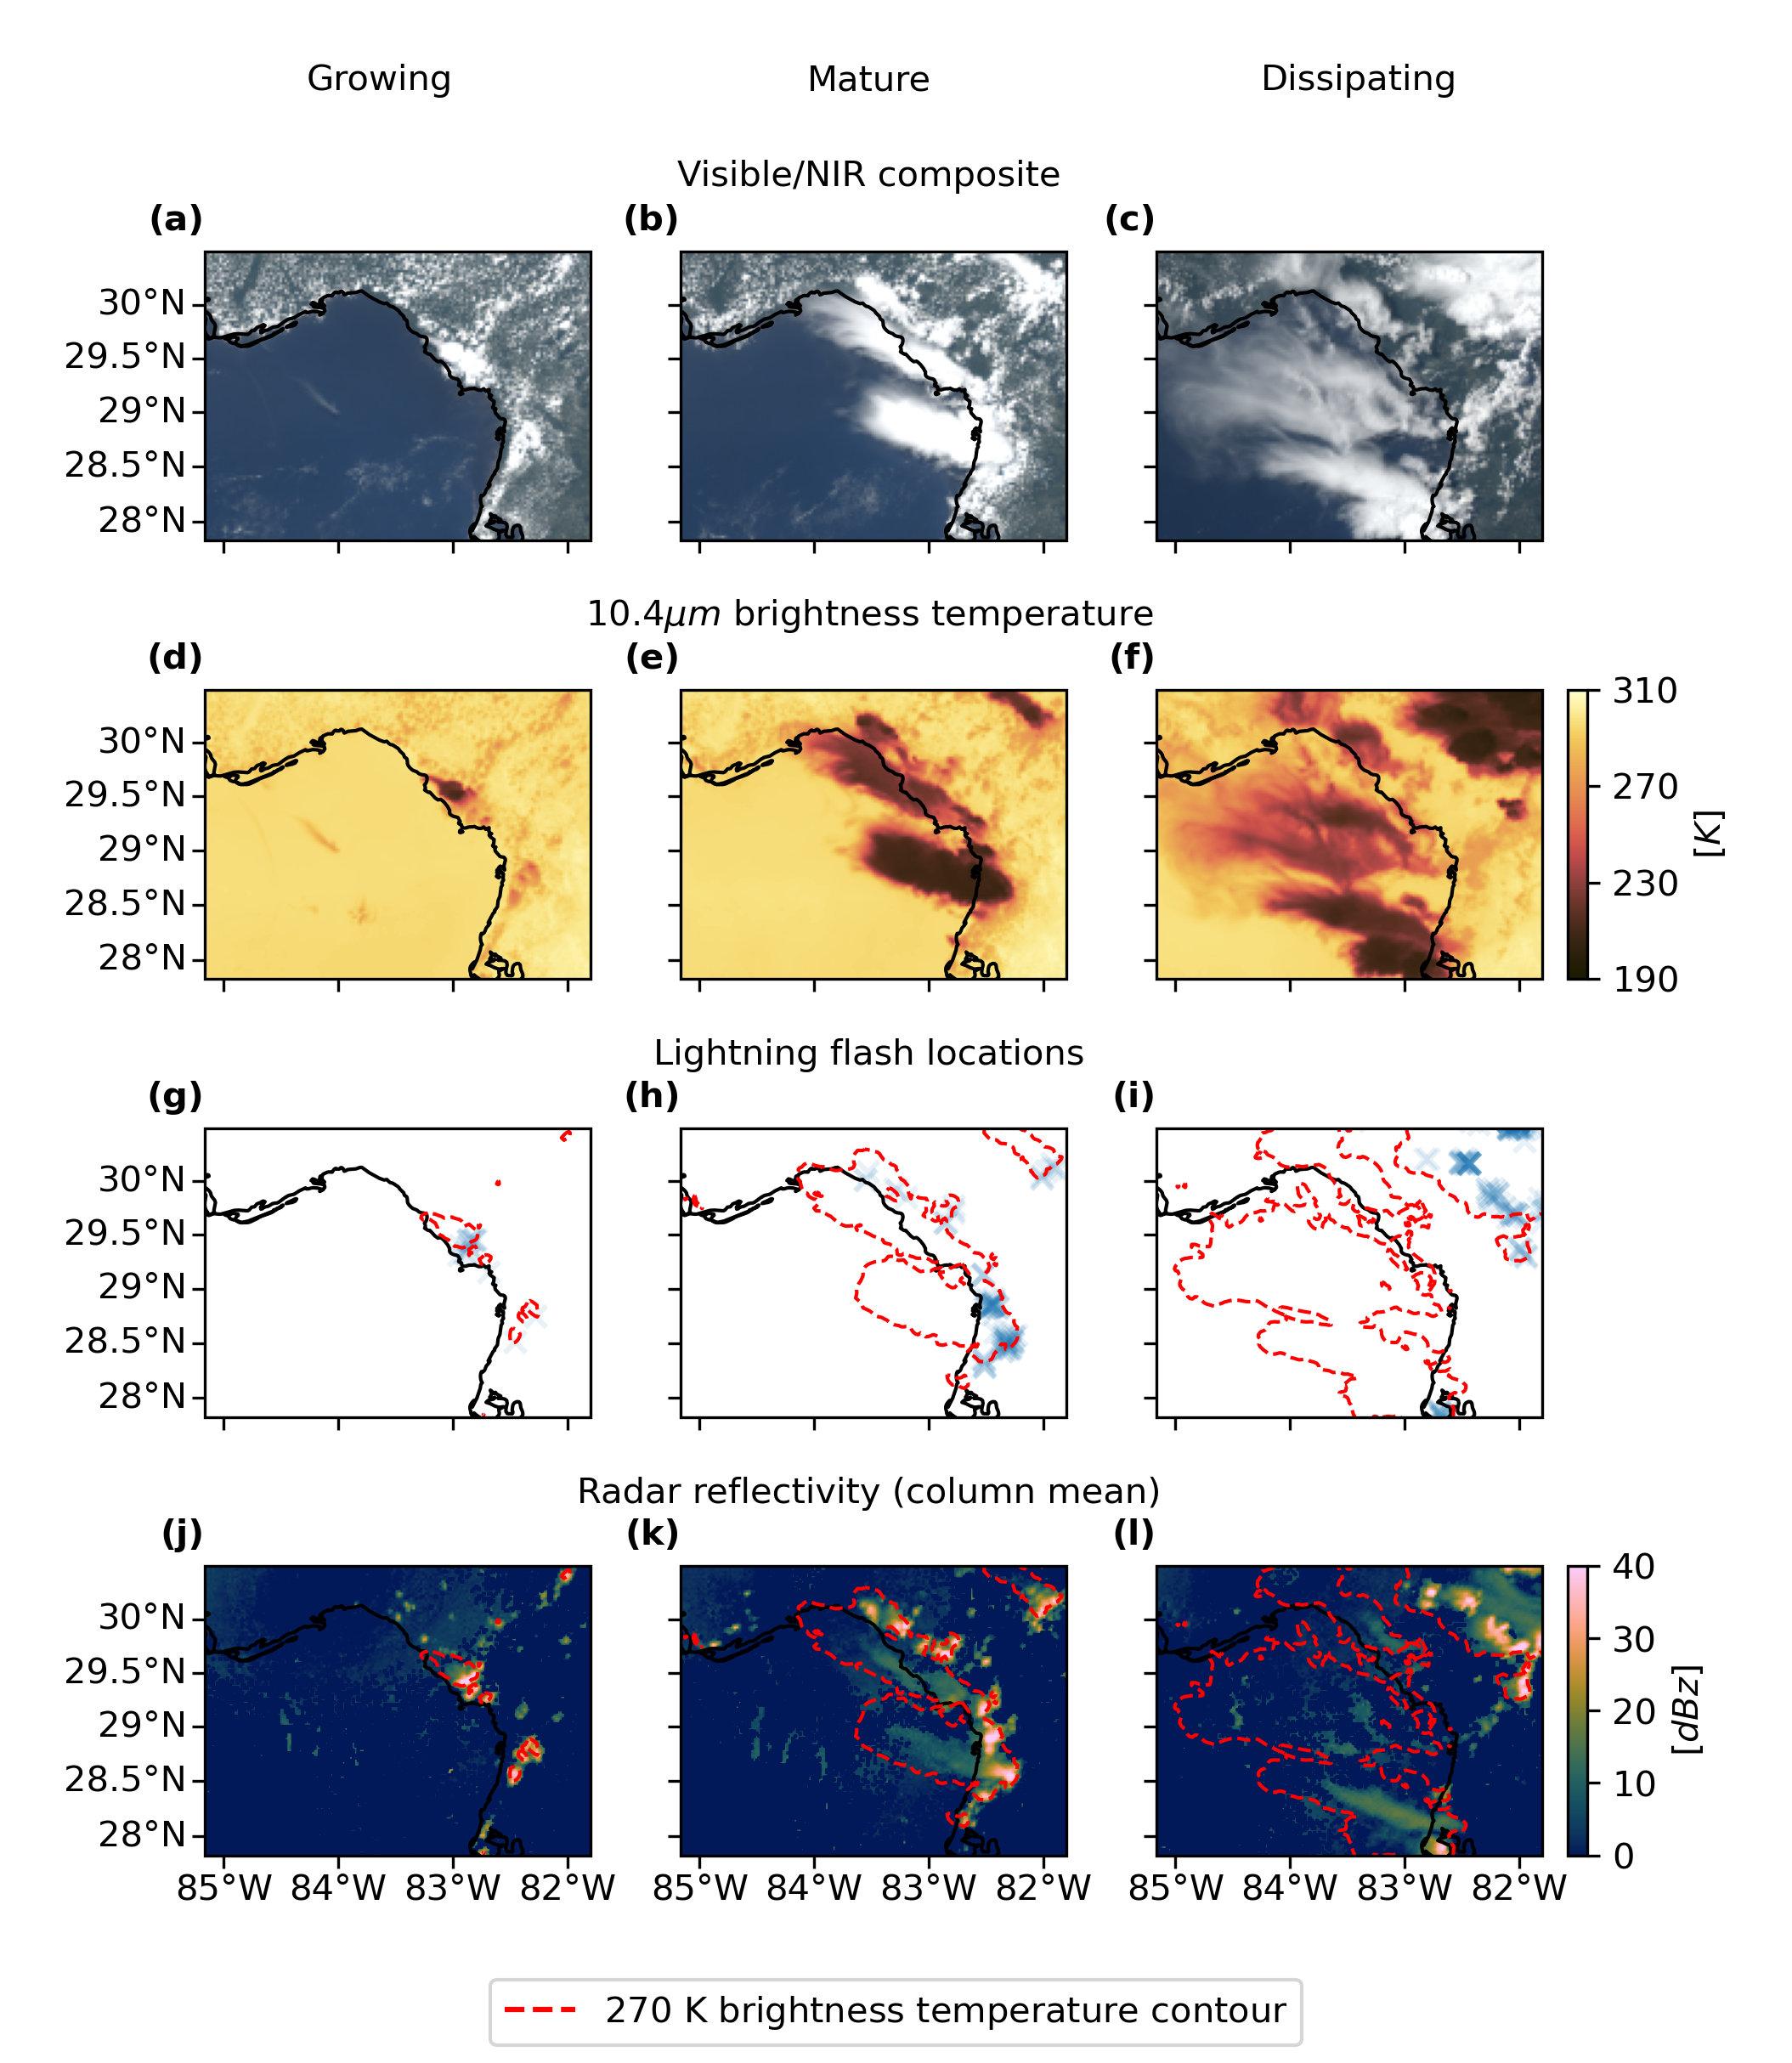
\includegraphics[width=\textwidth]{figures/chapter1_01.png}
    \caption[
    Observations of a cluster of \acrshort{dcc}s over North-West Florida throughout three stages of their lifecycle
    ]{
    Observations of a cluster of \acrshort{dcc}s over North-West Florida throughout three stages of their lifecycle. This cluster of \acrshort{dcc}s occurred on the afternoon of 19\textsuperscript{th} June 2018. The "growing" column was observed at 17:00 \acrshort{utc}, the "mature" column at 19:00 \acrshort{utc}, and the dissipating column at 21:00 \acrshort{utc}. The four rows show observations of \acrshort{abi} visible/\acrshort{nir} composites (a,b,c), and 10.4\,\unit{\mu m} \acrshort{bt} (d,e,f); lightning flash locations observed by \acrshort{glm} (g,h,i), and column mean radar reflectivity observed by \acrshort{nexrad} (j,k,l). Note that, unless otherwise specified, this case study is used for all subsequent figures in this chapter.
    }
    \label{fig:compare_sat_radar_glm}
\end{figure}

Sequences of images from satellite instruments have been used to detect and track the motion of \acrshort{dcc}s and tropical storms since the earliest geostationary weather satellites \citep{menzel_cloud_2001}.
Whereas early detection and tracking were performed by hand, numerous algorithms have been developed for the purpose of performing this task automatically, and are widely used for both forecasting and research purposes \citep[e.g.][]{mecikalski_use_2011, senf_characterization_2015, senf_satellite-based_2017, feng_life_2012, feng_spatiotemporal_2019, zinner_cb-tram:_2008}.
There is a continual effort both to improve existing algorithms and develop new methods to support these activities.
However, it is important to understand the differences in observations of \acrshort{dcc}s from satellite imagery to those of other sources, particularly radar and lightning observations.

Visible and \acrshort{ir} imagery from modern geostationary weather satellite instruments provide unique observations of \acrshort{dcc}s and their surrounding environment.
Figure~\ref{fig:compare_sat_radar_glm} compares observations of \acrshort{dcc}s throughout three different stages of their lifecycle between satellite visible and \acrshort{ir} imagery, doppler cloud radar and lightning flash observations.
Composite \acrshort{rgb} images from a combination of visible and \acrshort{nir} channels aboard the \acrshort{abi} show a.: small, isolated cores during the growing phase; b.: a large area of optically thick anvil during the mature phase, and c.: a large area of optically thin anvil cloud during the dissipating phase.
\acrshort{bt} imagery from the \acrshort{abi} 10.4\,\unit{\mu m} channel displays d.: rapidly cooling cores; e.: a large, cold anvil cloud, and f.: warmer \acrshort{bt}s caused by thermal radiation from the surface penetrating the optically thin dissipating anvil. 
Lightning flash locations observed by the \acrshort{glm} (\acrshort{glm}) aboard \acrshort{goes}-16 show g.: low frequency during the growing phase; h.: high frequency during the mature phase, and i.: no lightning activity in the dissipating phase. 
Column mean radar reflectivity observed by \acrshort{nexrad} doppler cloud radar shows high radar reflectivity in the convective cores during the j. growing and k. mature phases, and no area of high radar reflectivity during the dissipating phase. 
The outline of the region of \acrshort{bt}s below 270\,\unit{K} observed by \acrshort{abi} is shown by the orange dashed contour over the \acrshort{glm} flash locations and \acrshort{nexrad} radar reflectivity to indicate their observations relative to the anvil cloud.

These instruments are capable of observing the entire extent of the anvil clouds associated with \acrshort{dcc}s over their entire lifecycle, even after convective activity has ceased (fig.~\ref{fig:compare_sat_radar_glm}\,f).
This is of particular importance due to the influence of anvil cloud radiative forcing on the climate, their response to temperature change \citep{bony_thermodynamic_2016, hartmann_tropical_2016, ceppi_cloud_2017, gasparini_what_2019} and possible feedbacks on subsequent convective activity \citep{varble_erroneous_2018}.
The newest generation of geostationary imaging satellites offers greater opportunities for the study of \acrshort{dcc}s due to their high spatial and temporal resolution -- allowing the detection and tracking of individual convective cores \citep{heikenfeld_tobac_2019} -- and also due to their high signal-to-noise ratio allowing research quality observations \citep{iacovazzi_goes-16_2020}.

The detection and tracking of \acrshort{dcc}s from satellite imagery remains challenging due to the inability to directly observe the convection that drives \acrshort{dcc}s using passive visible and \acrshort{ir} observations.
This is unlike radar and lightning observations, which can directly observe deep convection due to the strong correlations between core updraft intensity and radar reflectivity and polarisation \citep{austin_relation_1987, rosenfeld_general_1993, zipser_vertical_1994},  and lightning flash occurrence \citep{williams_relationship_1989, deierling_total_2008, wang_relationship_2017}.
Instead, a proxy for convective activity must be used to detect deep convection in visible/\acrshort{ir} satellite imagery.
The approaches used for this can generally be separated into two separate methods. 
Firstly, the use of thresholds on \acrshort{bt} (\acrshort{bt}) or other observed fields, which are capable of detecting \acrshort{dcc} anvil clouds \citep[e.g.][]{schmetz_monitoring_1997, hong_detection_2005, schroder_deep_2009, liang_integrated_2017, senf_size-resolved_2018}.
Secondly, the detection of rapidly growing cloud tops by observing changes in the anvil cloud-top radiative cooling, or by other similar approximations of cloud growth \citep{zinner_cb-tram:_2008, bedka_objective_2010, muller_novel_2019}.

Developing a detection method using either approach is made challenging by the dynamic nature of \acrshort{dcc}s themselves.
\acrshort{dcc} cores typically have diameters of around 10\,\unit{km}, and updraft velocities on the order of 10\,\unit{m s\textsuperscript{-1}} \citep{weisman_mesoscale_2015}, and exist for 1-3 hours \citep{chen_diurnal_1997}.
Large, mesoscale convective systems (consisting of multiple cores joined by a single large anvil \citep{roca_simple_2017}) may span areas several orders of magnitude larger than isolated \acrshort{dcc}s \citep{houze_mesoscale_2004}, and typically exist to 10-20 hours or longer \citep{chen_diurnal_1997}.
The life cycle of a \acrshort{dcc} can be split into three phases: an initiation or growing phase, a mature phase and a dissipating phase after the cessation of convective activity \citep{wall_life_2018}.
There exists a significant difference between the diurnal cycles of deep convection over the land and over the ocean, with observed \acrshort{dcc}s over land clustered towards the end of the day \citep{taylor_evaluating_2017}.

%f
\begin{figure}[t]
    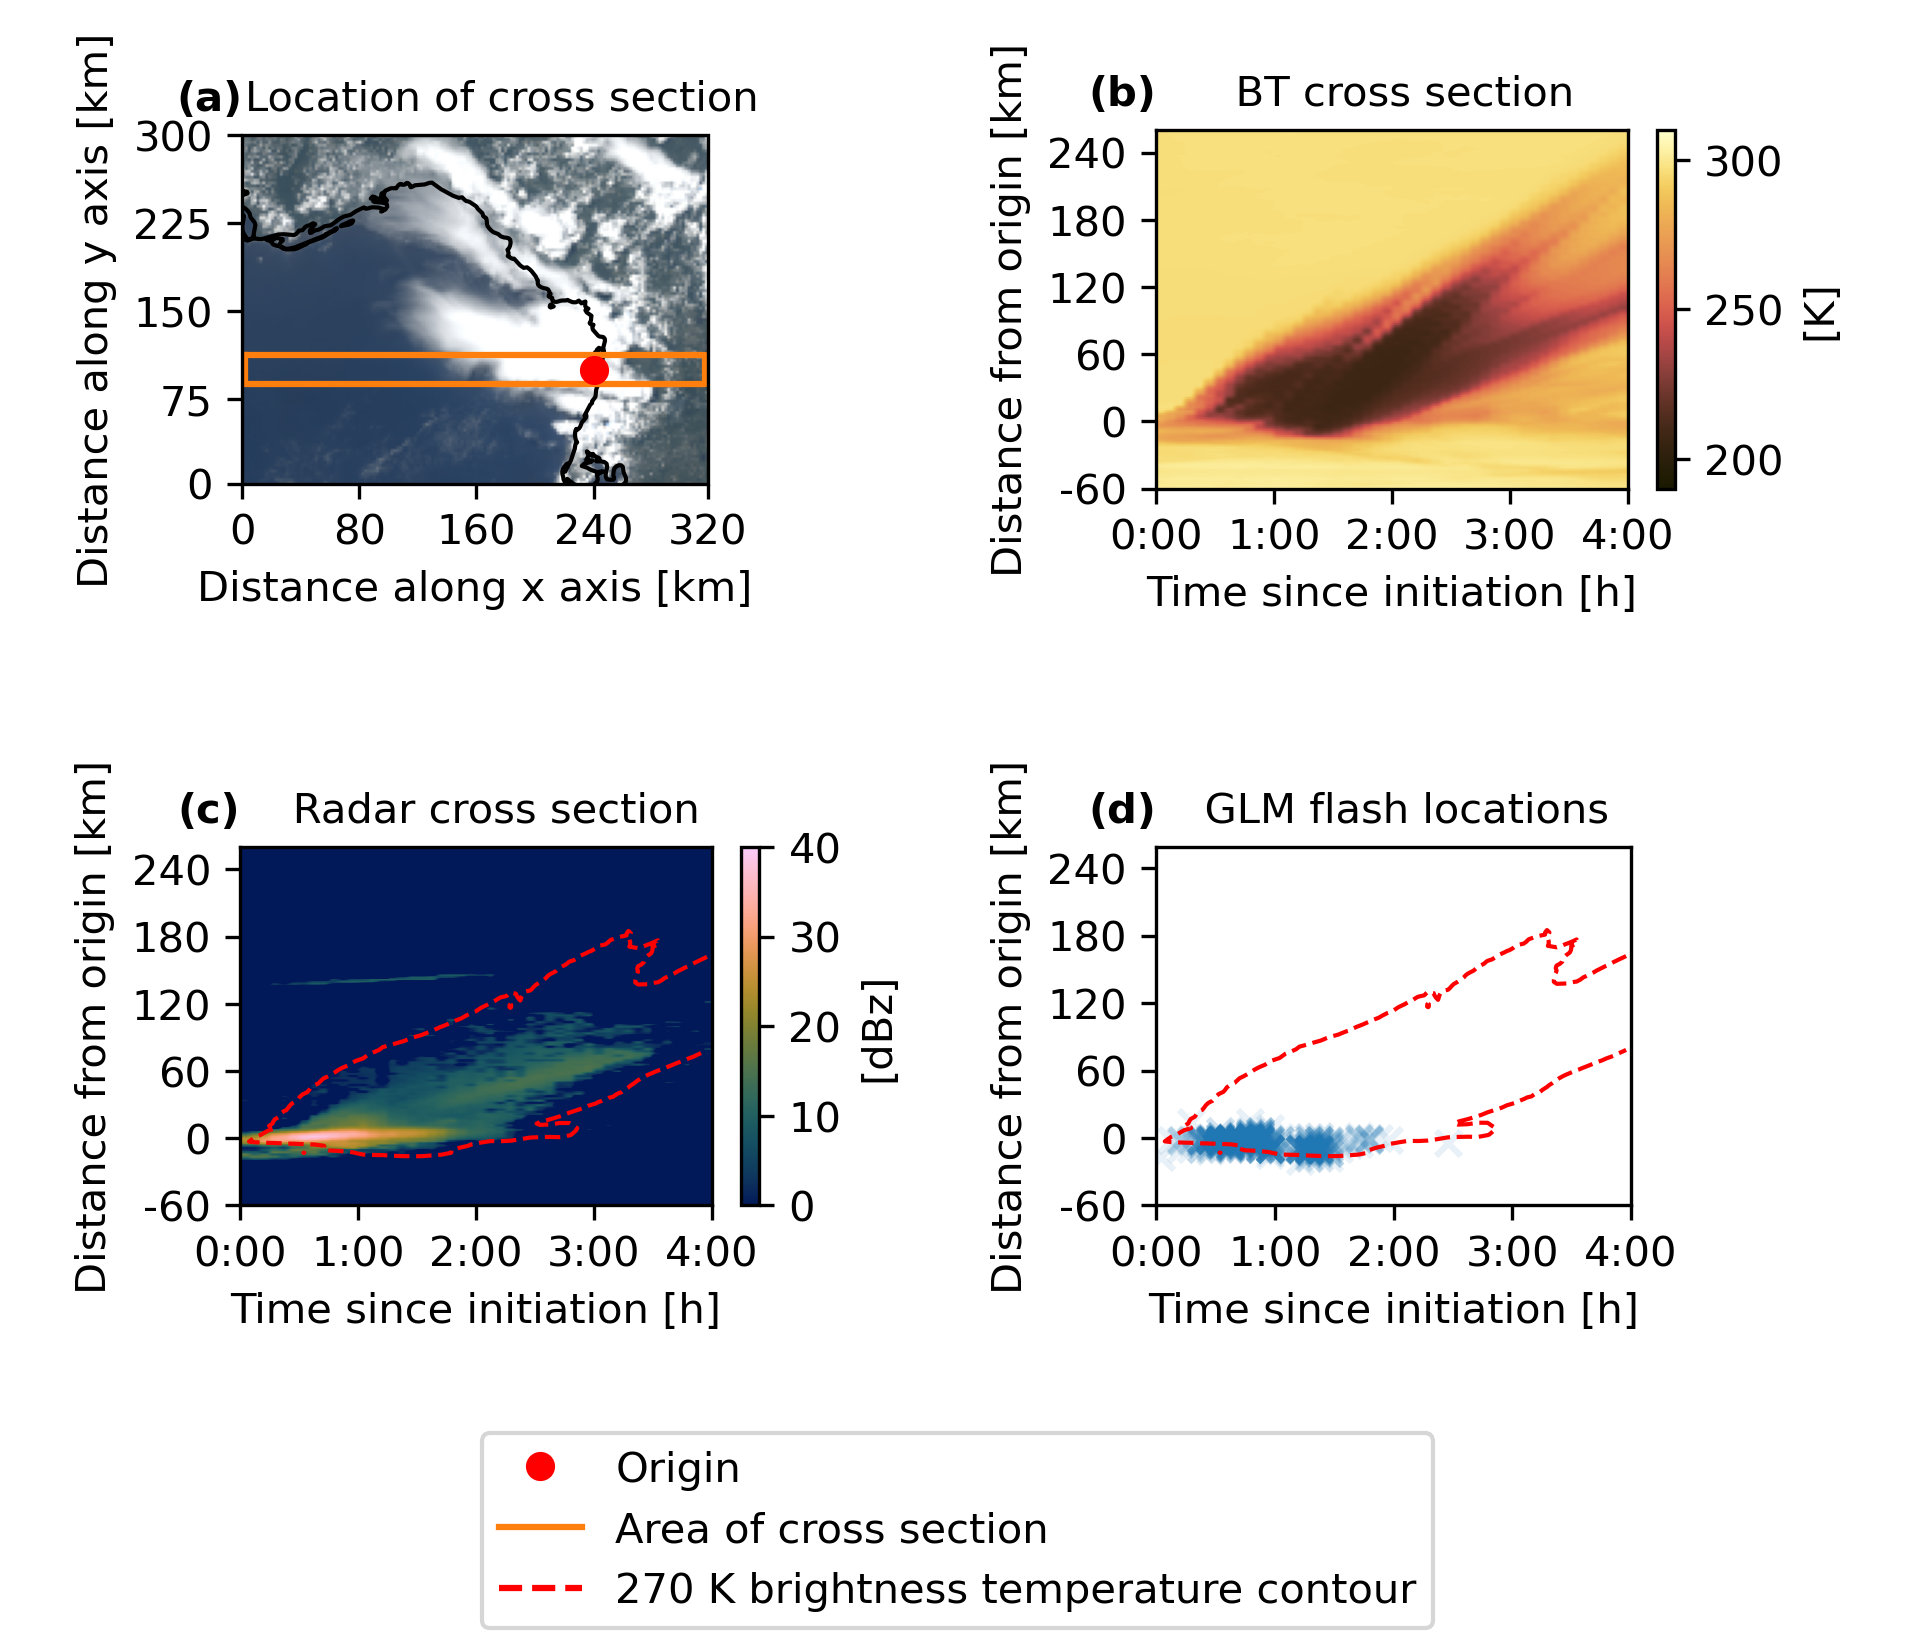
\includegraphics[width=\textwidth]{figures/chapter1_02.png}
    \caption[
    Cross sections of the \acrshort{dcc} observed in figure~\ref{fig:compare_sat_radar_glm} as they develop over time
    ]{
    Cross sections of the \acrshort{dcc} observed in figure~\ref{fig:compare_sat_radar_glm} as they develop over time. a.: The location of the cross-section within the observed \acrshort{dcc}. The mean of values is taken in the North-South axis. b.: \acrshort{abi} 10.8\,\unit{\mu m} \acrshort{bt}, showing rapid cooling for the first 30 minutes, followed by an expanding region of anvil cloud that begins to thin and warm after 2-3 hours. c.: Column mean radar reflectivity, showing the presence and location of the convective core. d.: Lightning flash locations observed by \acrshort{glm}, which closely match the core observed by \acrshort{nexrad}. Initiation occurred at 82.0\,\textdegree W 28.5\,\textdegree N at a time of 17:00 \acrshort{utc}.
    }
    \label{fig:dcc_over_time}
\end{figure}

The difficulties of detecting \acrshort{dcc}s using various proxy approaches are demonstrated by the cross-sections of an observed \acrshort{dcc} over time in fig.~\ref{fig:dcc_over_time}.
The observed \acrshort{bt} of the \acrshort{dcc} anvil cloud shows wide variation over time, with the anvil cloud warming due to dissipation after the end of convective activity.
This variety of observed temperatures leads to large differences in the chosen threshold value between different algorithms \citep[see discussion in][]{bennartz_convective_2012}.
This choice of the threshold value is further complicated due to the overlap in observed \acrshort{bt}s between \acrshort{dcc} anvils and non-convective clouds \citep{konduru_new_2013}.
As a result, any detection method using a \acrshort{bt} threshold must compromise between missed detection of \acrshort{dcc}s, or false detections of non-\acrshort{dcc} clouds.

The cooling of the cloud top is only visible for a short period during the initial phase of the \acrshort{dcc}, before the anvil cloud top reaches the tropopause temperature after approximately 30 minutes.
As a result, any method that solely relies on detecting the growth of the \acrshort{dcc} will be unable to detect the anvil cloud after this initial growth phase has ended.
While such algorithms provide accurate detection of these early phases of \acrshort{dcc} growth \citep{zinner_validation_2013}, they are unable to continue tracking the anvil cloud after convective activity is no longer observed.

\citet{fiolleau_algorithm_2013} identified this need to compromise on the accuracy of detecting \acrshort{dcc}s as a problem caused by the commonly used two-step framework for detecting and tracking \acrshort{dcc}s.
In this framework, \acrshort{dcc}s are first detected in individual images, and then linked together over time in sequences of images.
As a result, the detection method chosen must be capable of detecting \acrshort{dcc}s at each individual time step in order to track their entire lifecycle.
Instead \citet{fiolleau_algorithm_2013} implemented a single-step framework for mesoscale convective systems that treats a sequence of images as a "3D" volume, and performs detection and tracking simultaneously by applying a watershed method over both spatial and temporal dimensions.
Whereas this approach was successful for large, mesoscale systems, where the advection of the anvil is small compared to the overall anvil area, it is less capable of tracking small, rapidly moving convective cores.
To improve the tracking of small \acrshort{dcc}s, we have developed a semi-Lagrangian framework for single-step detection and tracking which accounts for the motion of \acrshort{dcc}s using optical flow.

By utilising the semi-Lagrangian framework, we are able to combine the best elements of both growth-based and threshold-based detection methods.
We show that it is possible to detect growing \acrshort{dcc}s to a high degree of accuracy using methods similar to those of \citet{zinner_cb-tram:_2008}, and then extend the detected \acrshort{dcc} over the entire anvil cloud using the "3D" watershed method of \citet{fiolleau_algorithm_2013}.
This framework reduces the compromise required between the rate of missed \acrshort{dcc}s and falsely detected \acrshort{dcc}s, improving the overall accuracy of our detection method compared to existing approaches.
Furthermore, this method allows the anvil cloud to be detected and tracked even after the region of cloud top cooling is no longer detected.
Finally, the "3D" method handles the merging and splitting of intersecting \acrshort{dcc}s by detecting all \acrshort{dcc}s that intersect at any point during their lifetime as a merged object.


% Performing such research is made difficult in particular by the wide range of scales -- both spatial and temporal -- required.
% Whereas deep convective cores required spatial resolution on kilometer scales and sub-hourly time steps to resolve, large scale balance in energetic and hydrological drivers appears on scales of thousands of kilometers and inter-annual periods.
% Geostationary satellite observations are uniquely capable of providing data on \acrshort{dcc}s spanning this range of scales.
% Furthermore, unlike observations from weather radars or lightning detectors, satellite imagery is capable of detecting \acrshort{dcc}s and their associated anvil clouds throughout their entire lifecycle (fig.~\ref{fig:compare_sat_radar_glm}).

% Accurate classification of \acrshort{dcc}s is vital for understanding their behaviour in response to environmental interactions and feedbacks.
% Detecting \acrshort{dcc}s using visible and \acrshort{ir} satellite imagery is challenging however as they cannot observe deep convection directly.
% Unlike weather radar, lightning detector and forecast and reanalysis model data, which provide properties directly linked to deep convection, proxy observations must be used to detect \acrshort{dcc}s in satellite images.
% We can separate the approaches to choosing a proxy for detecting \acrshort{dcc}s into two general categories:

% \begin{enumerate}
%     \item Passive methods, which involve one or more thresholds of observed fields including as \acrshort{lw} \acrshort{ir} \acrshort{bt}, outgoing \acrshort{lw} radiation, and retrieved properties such as cloud top height and effective cloud particle size.
%     \item Active methods, which observe changes in observations, either in changes over time or spatial gradients, which are indicative of deep convection.
% \end{enumerate}


% The accuracy of detection methods for \acrshort{dcc}s can be evaluated in terms of their false detection and missed detection rates (analogous to type 1 and type 2 errors respectively).
% The former occurs when an algorithm classifies a region as a \acrshort{dcc} when none is present, and the latter when an algorithm fails to classify a \acrshort{dcc} that is present.
% The choice of proxy for detecting deep convection is complicated by the innate dynamical nature of \acrshort{dcc}s themselves.
% As a result, there is no single proxy that is capable of accurately detecting \acrshort{dcc}s over their entire lifecycle.
% Instead, a compromise must be made between reducing false detections and missed detections.
% Passive detection proxies can generally be optimised for either a low false detection or low missed detection rate by changing the sensitivity of the threshold used, however this comes at a cost to the opposite measure of accuracy.
% Whereas active detection methods are generally capable of reducing both error rates, they are only capable of detecting \acrshort{dcc}s when active growth is observed, and therefore are only capable of making detections for a small proportion of the \acrshort{dcc} lifecycle.

% The need to compromise on accuracy is problematic for studying the interactions between multiple \acrshort{dcc}s, and both false and missed detections will cause spurious relationships to be discovered.
% A large reason for the compromise in accuracy is due to the two-stage framework used for detection and tracking in the majority of algorithms.
% In this framework, the algorithm first detects regions of \acrshort{dcc}s in individual images, and then tracks detected regions over time in sequences of images.
% As a result, the detection method chosen must be capable of detecting \acrshort{dcc}s in each individual image in order to track their entire lifecycle.
% Fiolleau and Roca identified this problem, and instead implemented a single-step framework for mesoscale convective systems that treats a sequence of images as a "3D" volume, and performs detection and tracking simultaneously by applying a watershed method over both spatial and temporal dimensions.
% Whereas this approach was successful for large, mesoscale systems, where the advection of the anvil is small compared to the over anvil area, it is less capable of tracking small, rapidly moving convective cores.
% To improve the tracking of small \acrshort{dcc}s, we have developed a semi-Lagrangian framework for single-step detection and tracking which accounts for the motion of \acrshort{dcc}s using optical flow.

% By utilising the semi-Lagrangian framework, we are able to combine the best elements of both active and passive detection methods.
% Growing deep convective cores are detected to a high degree of accuracy using an active detection method.
% This classification is then extended to the entirety of the associated anvil cloud by watershed segmentation over both spatial and temporal dimensions.
% This framework allows the anvil cloud to be detected and tracked even after the region of active growth is no longer detected.


\section{Data}

Three sources of data are used throughout this article.
Primarily, visible and \acrshort{ir} imagery from \acrshort{abi} aboard the \acrshort{goes}-16 weather satellite is used for the detection of \acrshort{dcc}s.
Secondarily, observations from the \acrshort{nexrad} weather radar network and the \acrshort{glm} (also aboard \acrshort{goes}-16) are used to assess and validate the tracking and detection method presented here.

%f
\begin{figure}[t]
    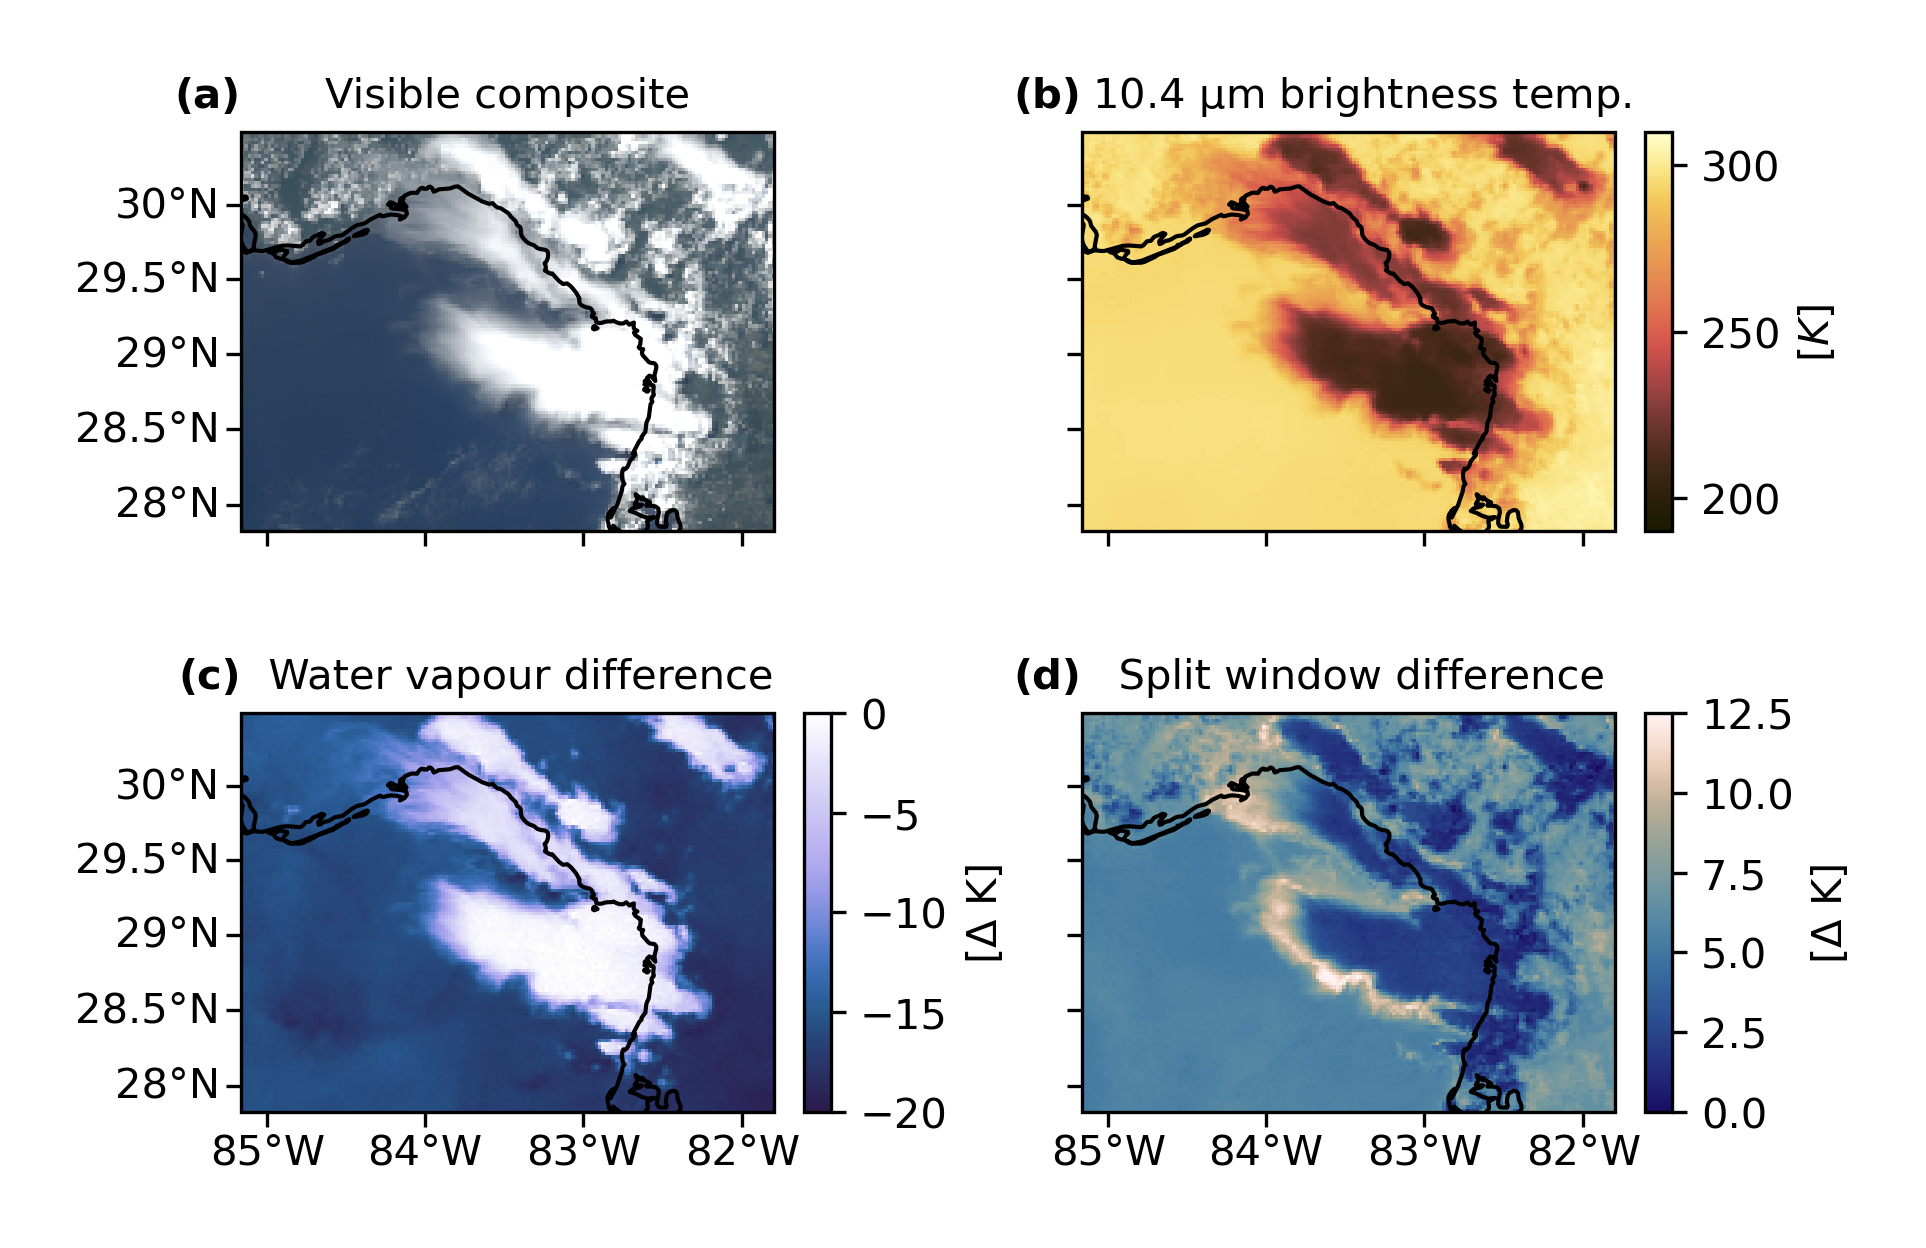
\includegraphics[width=\textwidth]{figures/chapter1_03.png}
    \caption[
    \acrshort{abi} channels and channel differences used with the detection and tracking algorithm
    ]{
    \acrshort{abi} channels and channel differences used with the detection and tracking algorithm. a.: A composite of visible and \acrshort{nir} channels. b.: The 10.4\,\unit{\mu m} \acrshort{bt}, or clean \acrshort{lw} window channel, which can differentiate clouds at all altitudes by their \acrshort{bt}. c.: the \acrshort{wvd} combination, of the 6.2\,\unit{\mu m} upper troposphere \acrshort{wv} channel minus the 7.3\,\unit{\mu m} lower troposphere \acrshort{wv} channel, which is strongly negative for clear sky and low cloud, but approaches positive values for thick, high clouds. d.: the \acrshort{swd} combination of the 10.4\,\unit{\mu m} clean \acrshort{lw} window channel minus the 12.4\,\unit{\mu m} dirty \acrshort{lw} window channel, which is near zero for thick clouds, around\,\unit{K} for clear skies and approximately 10\,\unit{K} for thin, ice clouds.
    }
    \label{fig:abi_channels}
\end{figure}

\subsection{Advanced Baseline Imager}


The \acrshort{abi} is a visible and \acrshort{ir} radiometer aboard the \acrshort{goes}-16 series of weather satellites \citep{schmit_closer_2016}.
\acrshort{goes}-16, also known as \acrshort{goes}-East, is situated in a geostationary orbit at 75.2\,\textdegree W above the equator, providing a field of view (or `Earth-disc') covering most of the western hemisphere, including all of South America and most of North America.
\acrshort{abi} has 16 channels operating in a range of spectral bands in the visible, \acrshort{nir} and thermal-\acrshort{ir}.
The majority of these channels have a resolution of 2\,\unit{km} at the sub-satellite point, although this reduces to approximately 3\,\unit{km} across most of the \acrshort{conus} due to the satellite viewing angle.
\acrshort{abi} operates in a flexible scan mode, imaging the continental US (\acrshort{conus}) once every 5 minutes, the full disc every 10 minutes (15 minutes prior to April 2019), and two mesoscale regions of approximately 2500 by 2500\,\unit{km} every minute.
Additionally, it is capable of scanning the full disc every five minutes if no other scans are performed.
This combination of high spatial and temporal resolution makes \acrshort{abi} suitable for detecting and tracking small and developing \acrshort{dcc}s, as well as providing the spatial coverage to also track large mesoscale convective systems \citep{heikenfeld_tobac_2019}.

Compared to older geostationary instruments, \acrshort{abi} has higher spatial and temporal resolution, more channels in both the \acrshort{lw} \acrshort{ir} window spectrum and the \acrshort{lw} \acrshort{ir} \acrshort{wv} spectrum, and low noise (table \ref{table:abi_comparison}) \citep{iacovazzi_goes-16_2020}.
This, combined with many of the channels being derived from those aboard the Visible Infrared Imaging Radiometer Suite, make the data from \acrshort{abi} more suitable for research purposes than that from older instruments \citep{heidinger_chapter_2020}.
A number of artifacts are known to occur in \acrshort{abi} imagery \citep{gunshor_goes-r_2020}.
Although the majority of these artifacts are removed using the data quality flag associated with the \acrshort{abi} data, we have found a number of cases in which bad detector stripes (described in section 3.2 of \citealp{gunshor_goes-r_2020}) are not flagged in the data, and so detection and tracking of \acrshort{dcc}s has not been performed during the time periods these artifacts occurred.

In this chapter, we have used the \acrshort{abi} level 2 \acrshort{mcmip} which provides calibrated reflectances and \acrshort{bt}s for all \acrshort{abi} channels on a common grid \citep{schmit_chapter_2020}, using the 5-minute frequency imagery provided over the \acrshort{conus} region.
The case study shown in the figures throughout this paper is for a subset of the \acrshort{conus} scan region centred at 83.7\,\textdegree W, 29.2\,\textdegree N, over the time period of 18:00:00 to midnight \acrshort{utc} on the 19th June 2018.
Validation was performed on a subset of the \acrshort{conus} scan region from 114 to 76\,\textdegree W and 24 to 45\,\textdegree N over the entirety of 2018.
All data has been sourced through the National Oceanic and Atmospheric Administration Big Data Program.

%t
\begin{table}[t]
\centering
\begin{tabular}{lrrr}
\tophline
Instrument                                              & \acrshort{abi}   & \acrshort{seviri}    & Imager \\
\middlehline
Temporal resolution (\unit{minutes})                    & 5     & 15        & 30 \\
Nadir spatial resolution (\unit{k m})                   & 2     & 3         & 4 (8 for \acrshort{wv}) \\
Number of \acrshort{ir} \acrshort{lw} window channels                         & 3     & 2         & 2 \\
Number of \acrshort{ir} \acrshort{wv} channels                                & 3     & 2         & 1 \\
Noise equivalent temperature  (\unit{K} @ 300\,\unit{K})  & 0.1   & 0.25      & 0.09 \\
\bottomhline
\end{tabular}
\caption[
Comparison of data from \acrshort{abi} to that from older geostationary instruments
]{
Comparison of data from \acrshort{abi} to that from older geostationary instruments\; \acrshort{seviri} aboard the second generation meteosat satellites, and the imager aboard the second generation \acrshort{goes}.
} % Table Footnotes
\label{table:abi_comparison}
\end{table}


\subsubsection{Selection of \acrshort{abi} Channels and Channel Combinations}

In order to have an equal performance during both day and nighttime, a selection of \acrshort{lw} \acrshort{ir} \acrshort{abi} channels are used for the detection and tracking of \acrshort{dcc}s (see fig.~\ref{fig:abi_channels}). 
These channels consist of the long wave \acrshort{lw} clean and dirty window channels at 10.4\,\unit{\mu m} and 12.4\,\unit{\mu m} respectively, and the upper and lower troposphere \acrshort{wv} channels at 6.2\,\unit{\mu m} and 7.3\,\unit{\mu m} respectively.
Whereas the \acrshort{lw} window \acrshort{ir} \acrshort{bt} is commonly used for the detection of anvil clouds using threshold-based methods, we have decided not to use it for this purpose in this method due to the wide range of \acrshort{bt}s observed within anvil clouds, and the variance of anvil cloud temperature because of changes in tropopause temperature due to meteorology and latitude.
However, the information contained within this field is used for the optical flow calculation of the cloud motion field.

\begin{figure}[t]
    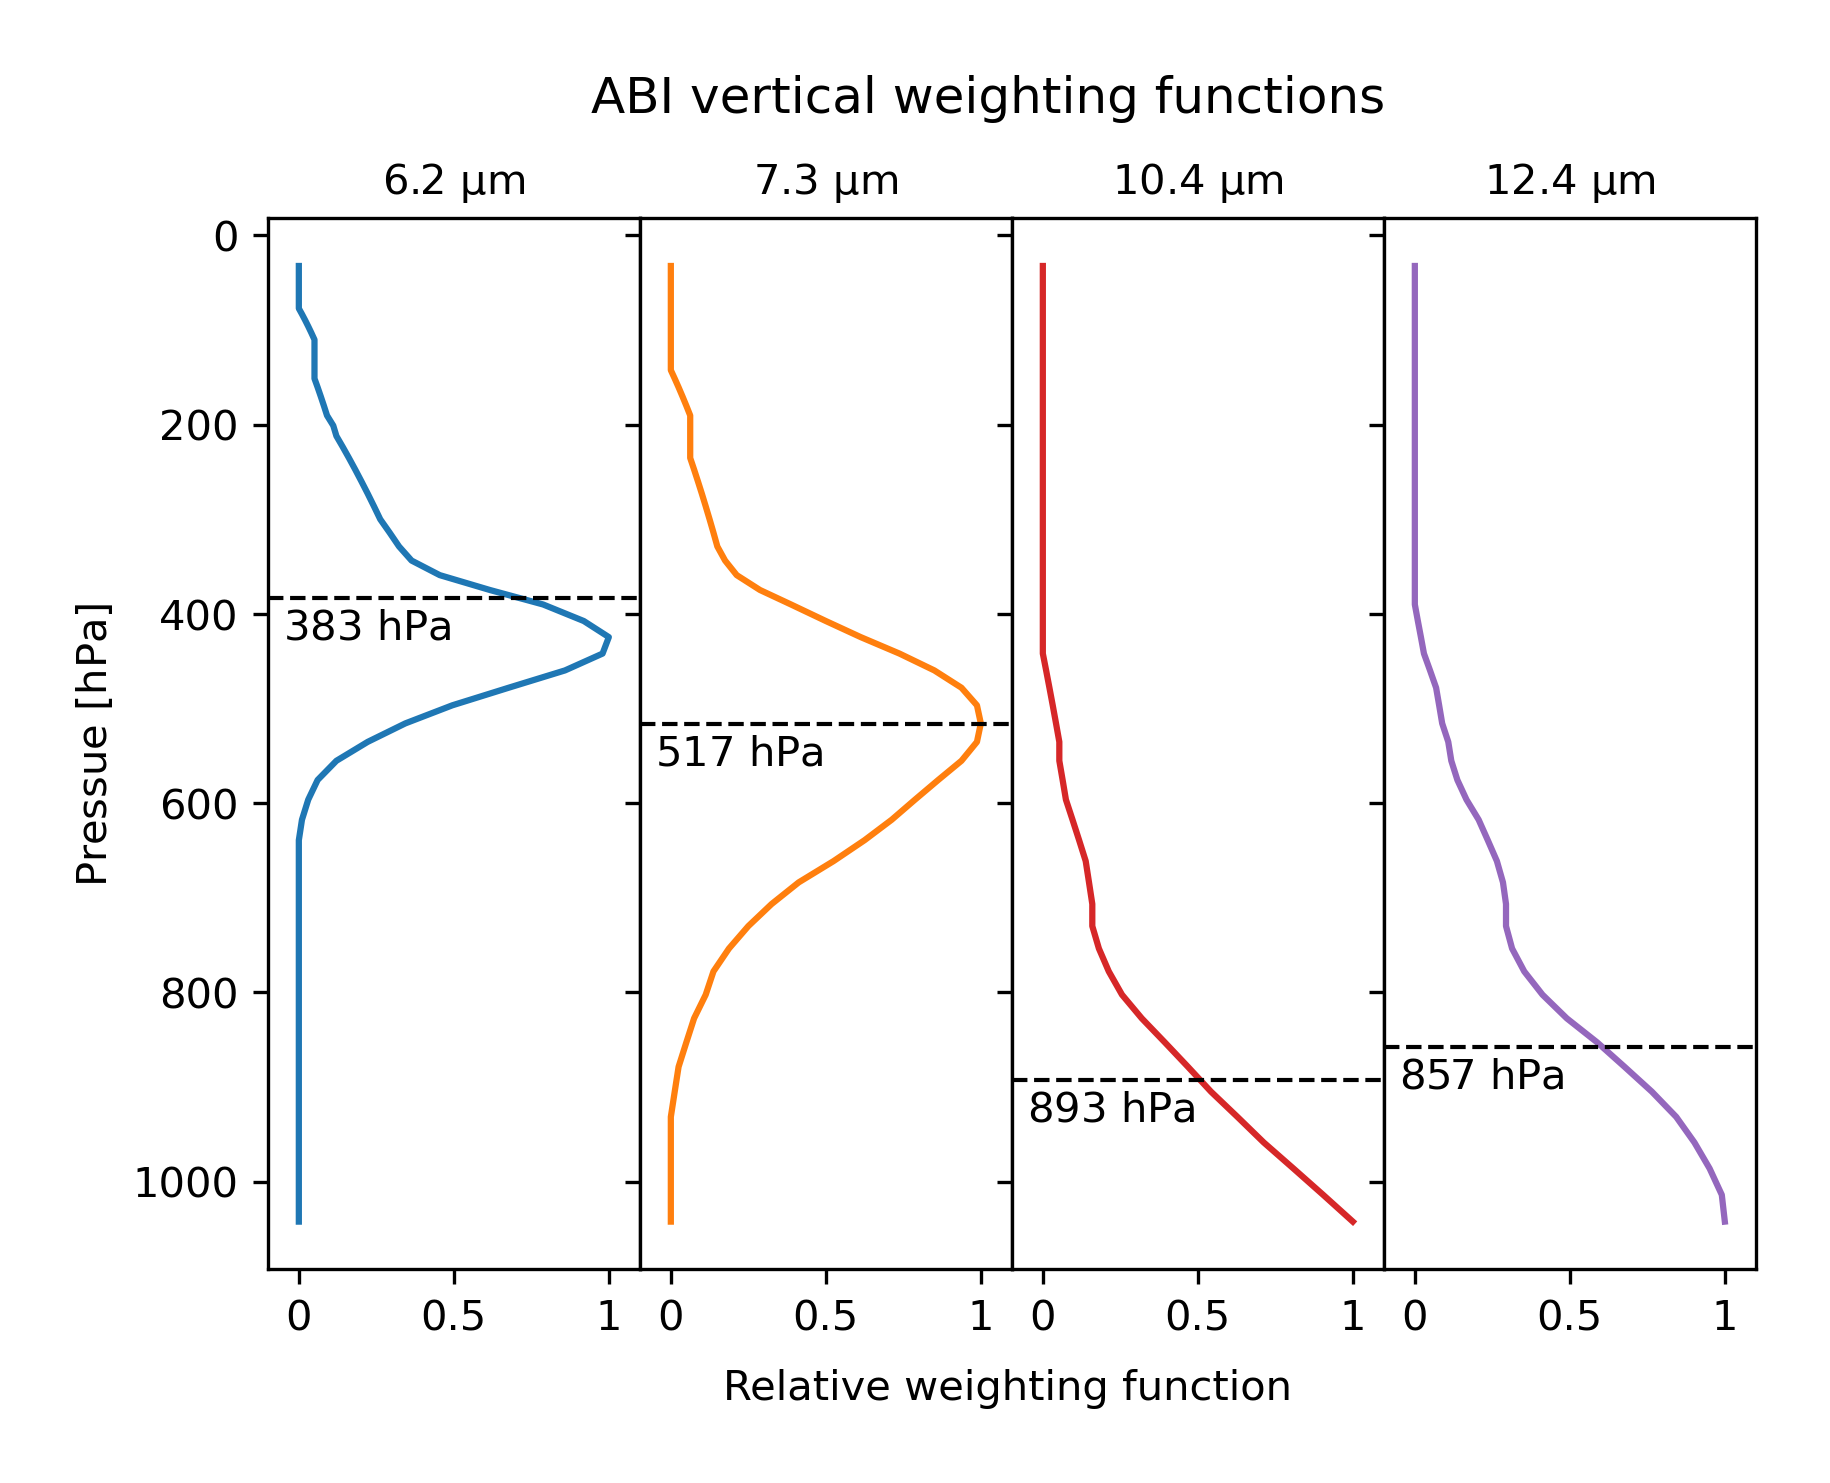
\includegraphics[width=\textwidth]{figures/chapter1_04.png}
    \caption[
    Clear sky vertical weighting functions for the 6.2, 7.3, 10.4 and 12.4\,\unit{\mu m} \acrshort{abi} channels
    ]{
    Clear sky vertical weighting functions for the 6.2, 7.3, 10.4 and 12.4\,\unit{\mu m} \acrshort{abi} channels calculated from rawinsonde profiles measured on 12:00:00 \acrshort{utc} 2020/08/10 at the Tampa RAOB station (KTBW - 72210). The dashed lines and associated pressure values show the weighted average emission height for each channel. Data from {https://cimss.ssec.wisc.edu/goes-wf/plot-viewer/\#/plot-viewer/plot/raob/abi16/default/20200810\_1200Z/72210}
    }
    \label{fig:abi_vertical_weighting}
\end{figure}

Two additional combinations of channels are used to detect areas of \acrshort{dcc} anvil. 
The \acrshort{wvd} combination (fig.~\ref{fig:abi_channels}\,c) of the upper troposphere \acrshort{wv} channel minus the lower troposphere \acrshort{wv} channel has been shown to provide a high detection rate for \acrshort{dcc}s \citep{muller_role_2018, muller_novel_2019}.
In clear sky or low cloud conditions, \acrshort{wvd} shows the temperature difference between the upper and lower troposphere of generally around -20\,\unit{K}. 
However, in the presence of high, thick clouds the 6.2\,\unit{\mu m} has an additional contribution from stratospheric \acrshort{wv} resulting in a warmer, and in extreme cases positive \acrshort{wvd} value \citep{schmetz_monitoring_1997}.
Because both the \acrshort{wv} channels are strongly absorbed by \acrshort{wv} in the lower troposphere, the \acrshort{wvd} field is not affected by surface and low altitude features and so provides a clear distinction between thick, high clouds and the background across a wide range of situations.
\citet{muller_novel_2019} found that a threshold of -5\,\unit{K} gave a high detection rate of anvil clouds.
Furthermore, as the \acrshort{wvd} values are relative to the lower stratosphere temperatures, this field is much less affected by location and meteorology than the \acrshort{lw} \acrshort{ir} channels.
However, the \acrshort{wvd} is still prone to the false detections of non-convective clouds when using a thresholding method as it cannot directly distinguish between thick, high-altitude clouds that are associated with deep convection and those that are not.

The Split Window Difference (\acrshort{swd}), consisting of the clean \acrshort{ir} window channel minus the dirty \acrshort{ir} window channel (fig.~\ref{fig:abi_channels}\,d), aids in the detection and separation of optically thin anvil cloud (including cirrus outflow) from optically thick anvil due to the difference in ice particle emissivity between these two channels \citep{heidinger_gazing_2009}.
As a result, this combination displays warm temperatures of around 10\,\unit{K} for thin, ice clouds, near 0\,\unit{K} for thick clouds, and approximately 5\,\unit{K} for clear skies due to the contribution of boundary layer \acrshort{wv}.
The \acrshort{swd} is, however, also sensitive to low-level clouds and low-level \acrshort{wv} concentrations, and so cannot be used alone to detect \acrshort{dcc}s.
It remains important to consider the \acrshort{swd} field due to the difficulty in separating anvil clouds from cirrus when using \acrshort{lw} \acrshort{ir} \acrshort{bt} alone \citep{hong_detection_2005}. 
By subtracting the \acrshort{swd} from the \acrshort{wvd} field, we can reduce the sensitivity of our detection scheme to cirrus clouds, reducing the rate of erroneous detections.
Further, adding the \acrshort{swd} field to the \acrshort{wvd} field can enhance the appearance of cirrus, enabling the detection of thin ice clouds associated with cirrus outflow and dissipating anvils.

Figure~\ref{fig:abi_vertical_weighting} shows the clear sky vertical weighing functions for the 6.2, 7.3, 10.4 and 12.4\,\unit{\mu m} \acrshort{abi} channels.
The weighting functions are calculated using a radiative transfer model with temperature and humidity profiles observed by rawinsonde observations on 12:00:00 \acrshort{utc} 2020/08/10 at the Tampa RAOB station (KTBW - 72210). 



\subsection{Geostationary Lightning Mapper}

The \acrshort{glm} is also mounted on \acrshort{goes}-16 and detects lightning flashes using an optical transient detector.
The optical transient detector utilises a single, narrow-band \acrshort{nir} channel centred on 777\,\unit{nm} \citep{orville_absolute_1984} to detect momentary changes in brightness associated with lightning events at a frequency of 400\,\unit{\mu s} \citep{christian_global_2003}, providing a 70\,\% minimum efficiency of detection \citep{goodman_goes-r_2013}.
\acrshort{glm} has the same field of view as the \acrshort{abi} instrument, albeit with a lower spatial resolution of 8\,\unit{km} at the sub-satellite point.

As lightning observations are strongly correlated with \acrshort{dcc}s, data from \acrshort{glm} is used to validate the detection of \acrshort{dcc}s using \acrshort{abi}.
The level 2 \acrshort{glm} Lightning Cluster-Filter Algorithm product provides a dataset of events, groups and flashes processed from the \acrshort{glm} data \citep{peterson_research_2019}, and filters artifacts from the level 1 \acrshort{glm} data \citep{peterson_removing_2020}.
From this dataset, we extract detected flashes as evidence of \acrshort{dcc} occurrence.
These locations are then processed by mapping their frequency onto the \acrshort{abi} grid for validation of the algorithm.

\subsection{Next Generation Radar}

\acrshort{nexrad}, also known by its technical name \acrshort{wsr88d}, is a network of weather radars operated by the National Weather Service across the USA \citep{crum_wsr-88d_1993}.
\acrshort{wsr88d} operates in the S-band spectrum, between 2700 and 3000\,\unit{MHz}.
\acrshort{nexrad} stations scan at a range of elevations, typically between 0.5\textdegree and 19.5\textdegree above horizontal, with a typical scan cycle taking between 4\,\sfrac{1}{2} and 6~minutes, comparable to the temporal sampling of \acrshort{abi} over the \acrshort{conus} region.

Cloud radar reflectivity is proportional to the droplet number density and the droplet radius to the sixth power, making it particularly sensitive to convective rainfall \citep{yau_short_1989}.
As a result, cloud radar observations are ideal for showing the locations of convective cores \citep{austin_relation_1987, rosenfeld_general_1993, zipser_vertical_1994}, and in this chapter it is used to qualitatively assess our ability to detect developing convective cores using \acrshort{abi}.
Level 2\acrshort{nexrad} radar reflectivity observations from multiple sites are gridded to the same resolution as \acrshort{abi}, and column mean reflectivity is calculated between the altitudes of 2.5 and 15\,\unit{k m}.

\section{Theory}

To better understand how \acrshort{dcc}s appear in \acrshort{goes} \acrshort{abi} observations, a series of experiments were performed using a radiative transfer model.
These experiments were performed using libRadTran v2.0.4 \citep{emde_libradtran_2016}, utilising the DISORT radiative transfer solver \citep{buras_new_2011} and the REPTRAN absorbtion parameterisation \citep{gasteiger_representative_2014}.
A tropical atmospheric profile was used to represent the atmospheric conditions under which deep convection typically occurs.
A complete list of the options used to set up the radiative transfer model across all simulations is provided in table \ref{table:libradtran}.

\begin{table}[t]
\centering
\begin{tabular}{lll}
\tophline
Option          & Value                 & Description                   \\ 
\middlehline
rte\_solver     & disort                & DISORT solver                 \\
source          & thermal               & thermal \acrshort{ir} spectra \\
wavelength      & 3000--15000           & 3--15\,\unit{\mu m}           \\
output\_user    & lambda edir eup uu    & wavelength, direct, diffuse   \\
                &                       &irradiance and all radiances   \\
zout            & 0 TOA                 & surface and \acrshort{toa}    \\
albedo          & 0.5                   & surface albedo                \\
umu             & -1.0, 1.0             & downward \& upward            \\
sza             & 0                     & solar zenith angle            \\
mol\_abs\_param & reptran fine          & REPTRAN parameterisation      \\
atmosphere\_file& afglt.dat             & tropical atmosphere profile   \\
\bottomhline
\end{tabular}
\caption[
    Selected options for the libRadTran simulations
    ]{
    Selected options for the libRadTran simulations.
    }
\label{table:libradtran}
\end{table}

In each of the simulations, a cloud layer is included in addition to these options to represent a \acrshort{dcc} in different phases of the lifecycle.
For liquid cloud droplets we use the Hu parameterisation \citep{hu_accurate_1993}, and for ice particles we use the Fu scheme \citep{fu_accurate_1996, fu_accurate_1998}. To show how the simulated clouds are observed by \acrshort{goes}-16, we calculate \acrshort{bt} from the simulated radiances, and then integrate over the spectral response function of each of the \acrshort{abi} channels.

\subsection{Observing growing convective cores}\label{sec:theory_core}

The first experiment aims to represent how a vertically developing \acrshort{dcc} core would appear in \acrshort{abi} observations.
To do so, we run a series of simulations with increasing cloud top heights between 1 and 15\,\unit{k m} at 1\,\unit{k m} intervals.
These cloud layers are given a base height of 0\,\unit{k m}, \acrshort{lwc} of 1,000\,\unit{g m^{-2}}, and droplet \acrshort{re} of 15\,\unit{\mu m}.
These values were chosen to represent typical conditions seen in a convective core.
Although we use liquid droplets at all altitudes, simulations with ice cloud droplets showed negligible differences for cloud layers of this thickness.

Figure~\ref{fig:cloud_height_spectra} shows \acrshort{bt} spectra for increasing cloud height, with the spectral response functions of the ten thermal \acrshort{ir} \acrshort{abi} channels plotted in the background.
With such a large \acrshort{lwc}, the \acrshort{bt} matches the \acrshort{ctt} apart from the absorption regions of CO\textsubscript{2} (4.2--4.5\,\unit{\mu m} and \>13.2\,\unit{\mu m}) and ozone (9.4--10.2\,\unit{\mu m}), and the \acrshort{wv} absorption for low-level clouds (5--8\,\unit{\mu m}).

The change in observed \acrshort{bt} with height for the 6.2, 7.3, 10.4, and 12.4\,\unit{\mu m} \acrshort{bt} channels along with the \acrshort{wvd} and \acrshort{swd} is plotted in Fig.~\ref{fig:cloud_height_channels}. 
Above 3\,\unit{k m }, the 10.4 and 12.4\,\unit{\mu m} channels show a constant decrease observed \acrshort{bt} at the moist pseudo-adiabatic lapse rate of 6\,\unit{K}.
Due to the contribution of \acrshort{wv} to the 6.2 and 7.3\,\unit{\mu m} channels at lower \acrshort{cth}, the \acrshort{wvd} shows the most response to vertical development between 6 and 10\,\unit{k m}.
The \acrshort{swd} shows a response to clouds developing at a low altitude.
It has been proposed that this can be used to detect the onset of convection in clear sky conditions before other observations, such as cloud radars \citep{lindsey_use_2014, lindsey_using_2018}.

Figure~\ref{fig:cloud_height_cooling_rates} shows the change in \acrshort{bt} observed over a vertically developing core in units of \unit{K minute^{-1}/m s^{-1}} (i.e. the \acrshort{bt} change per minute, per \unit{m s^{-1}} of vertical development rate).
Although this is an odd choice of unit, it is used to better compare the observed change in \acrshort{bt} by a geostationary satellite (measured in \unit{K}, with a typical sampling time on the order of minutes), to the vertical velocity of the cloud top (typically measured in \unit{m s^{-1}}.
Above 3\,\unit{km}, the 10.4\,\unit{\mu m} \acrshort{bt} shows a consistent cooling rate of 0.4\,\unit{K minute^{-1}}.
\citet{roberts_nowcasting_2003} found a threshold for severe convection of 8\,\unit{K} cooling over 15~minutes, or approximately 0.5\,\unit{K minute^{-1}}, which would represent a cloud top vertical velocity of 1.25\,\unit{m s^{-1}} according to our simulation.
The \acrshort{wvd} shows a maximum rate of change between 7 and 8\,\unit{k m}, with a warming rate of half the magnitude of the \acrshort{bt} cooling rate.

Overall, we see from this experiment that the 10.4\,\unit{\mu m} \acrshort{bt} channel from \acrshort{abi} can be used to clearly identify a vertically developing core across a wide range of altitudes.
On the other hand, the \acrshort{wvd} is only sensitive to vertically developing clouds in a narrower range of altitudes, and shows a weaker rate of \acrshort{bt} change.
However, this sensitivity to vertical development at a mid to high altitude may be helpful in distinguishing between \acrshort{dcc}s and other, vertically developed clouds at lower altitudes, such as cumulus congestus.

\begin{figure}[t]
    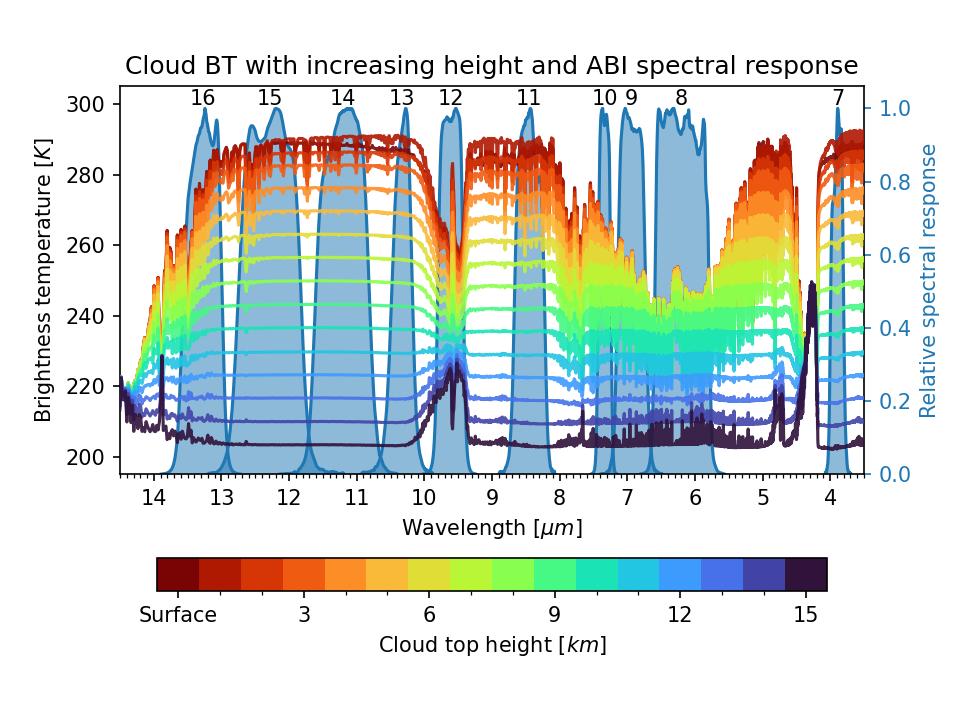
\includegraphics[width=\textwidth]{figures/chapter1_05.png}
    \caption[
    \acrshort{toa} \acrshort{bt} spectra for a simulated cloud representing a \acrshort{dcc} core at heights between 1 and 15\,\unit{k m}
    ]{
    \acrshort{toa} \acrshort{bt} spectra for a simulated cloud representing a \acrshort{dcc} core at heights between 1 and 15\,\unit{k m}. The filled blue areas in the background show the relative spectral response functions for each of the \acrshort{lw} \acrshort{abi} channels.
    }
    \label{fig:cloud_height_spectra}
\end{figure}

\begin{figure}[t]
    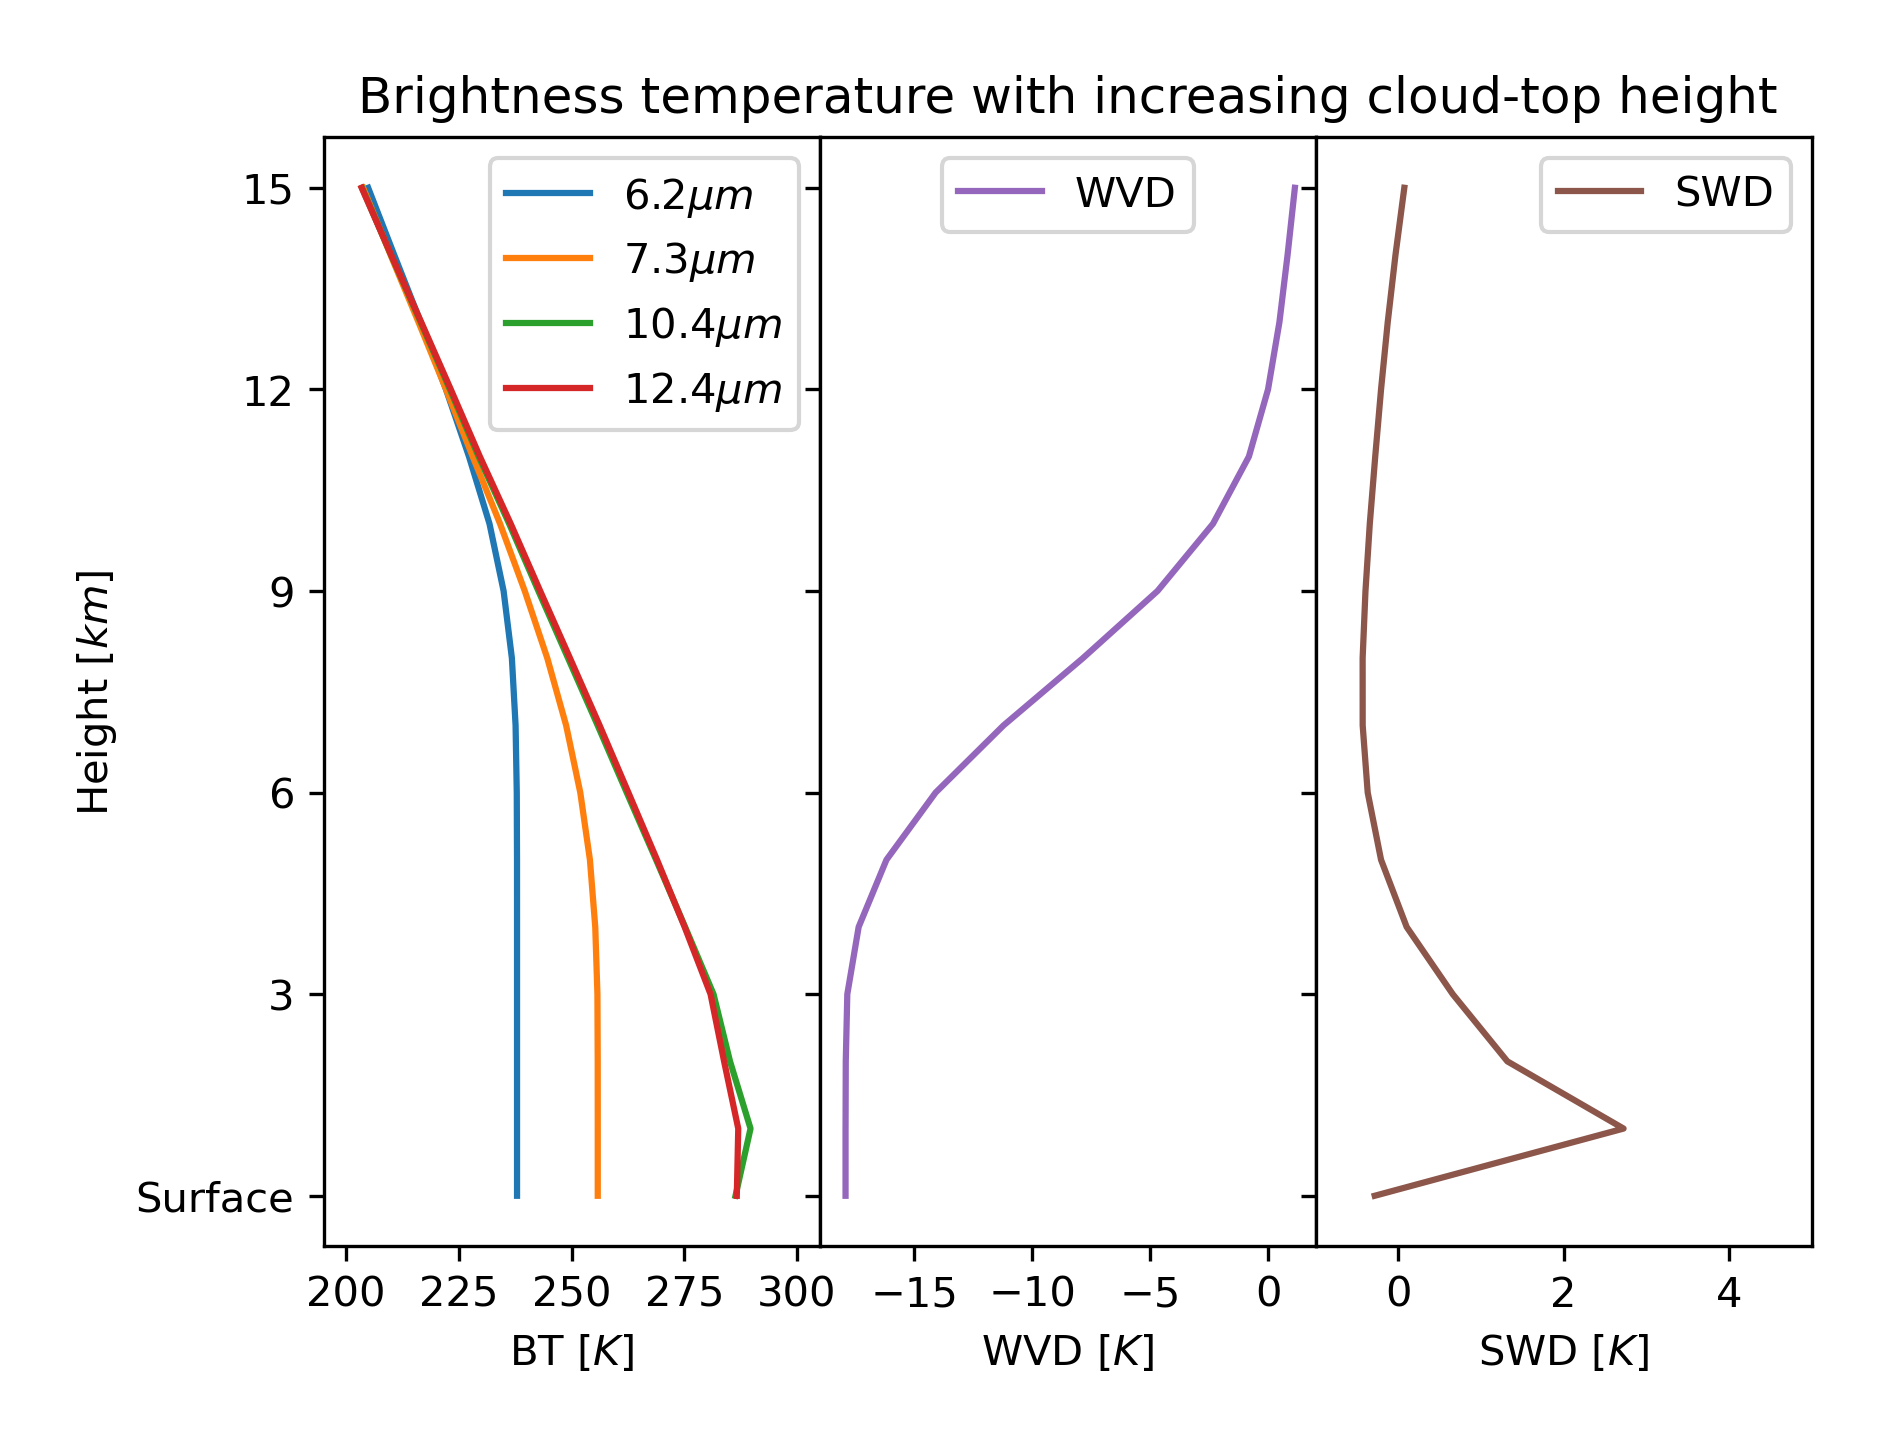
\includegraphics[width=\textwidth]{figures/chapter1_06.png}
    \caption[
    Simulated observations of the 6.2, 7.3, 10.4 and 12.4\,\unit{\mu m} \acrshort{abi} channels, \acrshort{wvd} and \acrshort{swd} for a \acrshort{dcc} core of increasing height
    ]{
    Simulated observations of the 6.2, 7.3, 10.4 and 12.4\,\unit{\mu m} \acrshort{abi} channels, \acrshort{wvd} and \acrshort{swd} for a \acrshort{dcc} core of increasing height.
    }
    \label{fig:cloud_height_channels}
\end{figure}

\begin{figure}[t]
    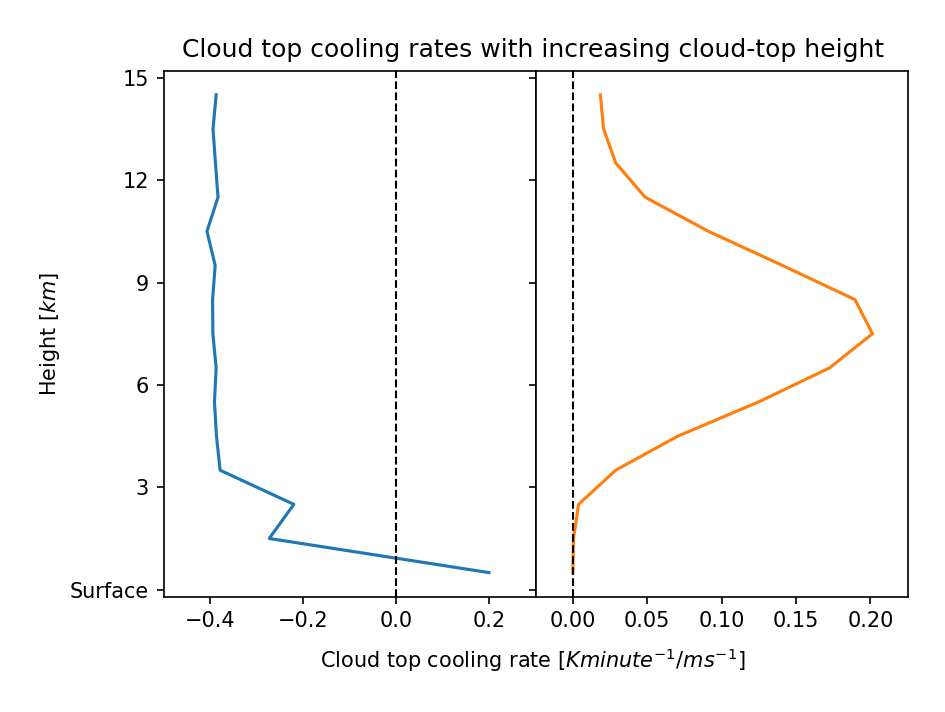
\includegraphics[width=\textwidth]{figures/chapter1_07.png}
    \caption[
    Simulated observed cooling rates of the 10.4\,\unit{\mu m} \acrshort{abi} channels and the \acrshort{wvd} combination for a convective core growing at a rate of 1\,\unit{m s^{-1}}
    ]{
    Simulated observed cooling rates of the 10.4\,\unit{\mu m} \acrshort{abi} channels and the \acrshort{wvd} combination for a convective core growing at a rate of 1\,\unit{m s^{-1}}.
    }
    \label{fig:cloud_height_cooling_rates}
\end{figure}

\subsection{Observing anvil clouds}

In the second experiment, we investigate how anvil clouds of different \acrshort{od} appear in \acrshort{abi} observations.
The simulations were run with an ice cloud with \acrshort{cth} at 14\,\unit{k m}, cloud base height at 12\,\unit{km} and cloud top \acrshort{re} of 20\,\unit{\mu m}, aiming to represent the typical properties of a dissipating anvil cloud \citep{sokol_tropical_2020}.
This simulation was then run for a range of \acrshort{od} between 0.125 and 10, with intervals of 0.125 between 0.125 and 1, 0.25 between 1 and 2, 0.5 between 2 and 5, and 1 between 5 and 10.

\acrshort{bt} spectra for these simulations are shown in Fig.~\ref{fig:optical_depth_spectra}, along with the \acrshort{abi} spectral response functions as in Fig.~\ref{fig:cloud_height_spectra}.
As before, we see absorption due to CO\textsubscript{2}, ozone, and \acrshort{wv}.
Unlike the simulations in section \ref{sec:theory_core} however, we see a difference in the \acrshort{bt} spectra across the \acrshort{lw} window (10--13\,\unit{\mu m}) for clouds with \acrshort{od} between 0 and 2, with colder \acrshort{bt} at longer wavelengths.
This is due to the difference in ice emissivity across this range of wavelengths \citep{fu_radiation_2015}.
As the emissivity of ice particles reduces for wavelengths at 10\,\unit{\mu m} and below there is a greater contribution from the atmosphere below the cloud layer and, as a result, warmer \acrshort{bt}s are observed.
It should be noted that this difference is dependent on the size of the ice particles, with smaller \acrshort{re} resulting in a larger difference in emissivity \citep{dubuisson_sensitivity_2008}.

Figure~\ref{fig:optical_depth_channels} shows simulated \acrshort{abi} observations for the 6.2, 7.3, 10.4, and 12.4\,\unit{\mu m} \acrshort{bt} channels, the \acrshort{wvd} and the \acrshort{swd} for a range of \acrshort{od} between 0.1 and 10.
At high \acrshort{od}, all channels show a cold \acrshort{bt} close to that of the \acrshort{ctt}, however, for \acrshort{od} below 3, the increased contribution from the atmosphere below results in warmer \acrshort{bt}.
The \acrshort{wvd} similarly shows a more negative \acrshort{bt} difference at \acrshort{od} below 3, with a continual decrease for smaller \acrshort{od}.
The \acrshort{swd} however shows an increasingly positive \acrshort{bt} difference for \acrshort{od} below 5, peaking at 10\,\unit{K} around 1~\acrshort{od}.
However, below this \acrshort{od} the \acrshort{swd} decreases towards smaller positive values.
As a result, the \acrshort{swd} has the potential to detect thin anvil cirrus at much low \acrshort{od} than \acrshort{bt} channels or \acrshort{wvd}, down to values around 0.25~\acrfull{od}.

\begin{figure}[t]
    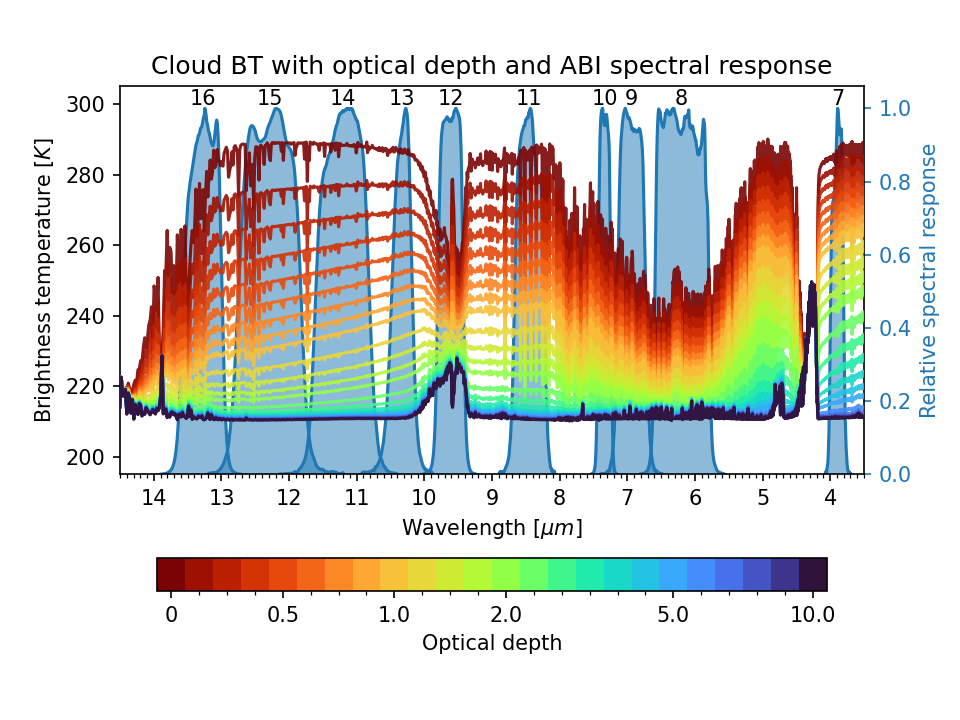
\includegraphics[width=\textwidth]{figures/chapter1_08.png}
    \caption[
    \acrshort{toa} \acrshort{bt} spectra for a simulated anvil cloud with optical thickness between 0 and 10
    ]{
    \acrshort{toa} \acrshort{bt} spectra for a simulated anvil cloud with optical thickness between 0 and 10. 
    }
    \label{fig:optical_depth_spectra}
\end{figure}

\begin{figure}[t]
    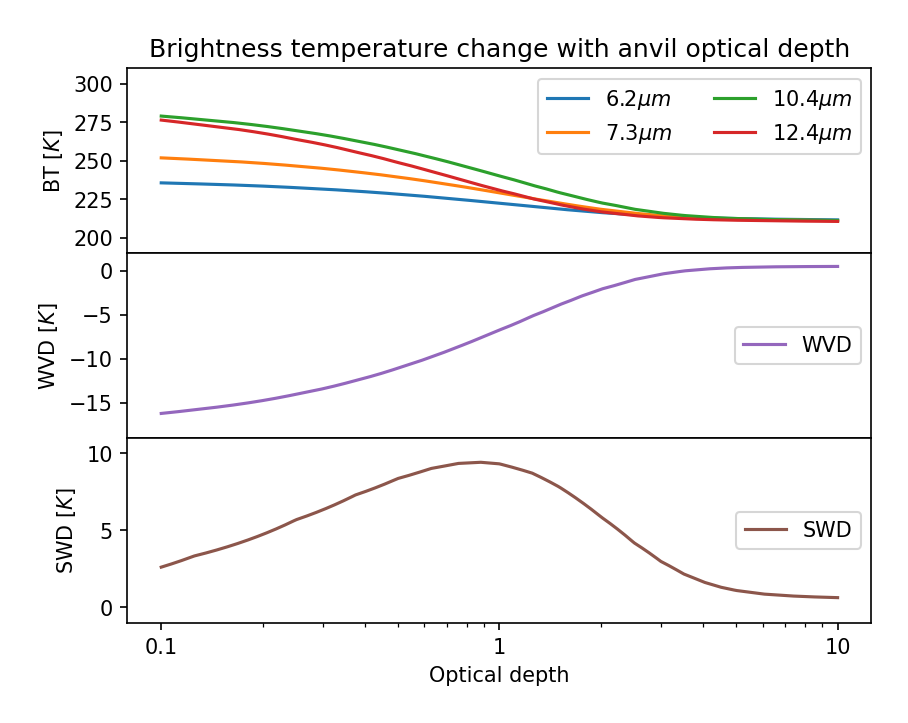
\includegraphics[width=\textwidth]{figures/chapter1_09.png}
    \caption[
    Simulated \acrshort{abi} \acrshort{bt} observations for a \acrshort{dcc} anvil of decreasing optical depth
    ]{
    Simulated \acrshort{abi} \acrshort{bt} observations for a \acrshort{dcc} anvil of decreasing optical depth for the 6.2, 7.3, 10.4, and 12.4\,\unit{\mu m} \acrshort{bt} channels, the \acrshort{wvd} and the \acrshort{swd}.
    }
    \label{fig:optical_depth_channels}
\end{figure}


\section{Method}

We present here a novel method for detecting and tracking both the growing cores and anvils clouds of \acrshort{dcc}s, consisting of the following steps:

\begin{enumerate}
    \item Ingest of \acrshort{lw} \acrshort{ir} \acrshort{bt} fields from geostationary satellite imagery, including calculation of \acrshort{wvd} and \acrshort{swd} fields from \acrshort{ir} \acrshort{wv} and \acrshort{lw} \acrshort{ir} window channels.
    \item Calculation of optical flow vectors to be used as an \textit{a priori} estimate of cloud motion for use in the semi-lagrangian framework.
    \item Detection of growing \acrshort{dcc} cores using cloud top cooling rate.
    \item Detection of thick and thin anvil clouds associated with detected cores using a semi-lagrangian "3D" watershedding method. 
    \item Grouping of cores into multi-core systems, calculation of statistics and validation using lightning observations.
\end{enumerate}



\subsection{Estimation of cloud motion vectors using optical flow}

\begin{figure}[t]
    \centering
    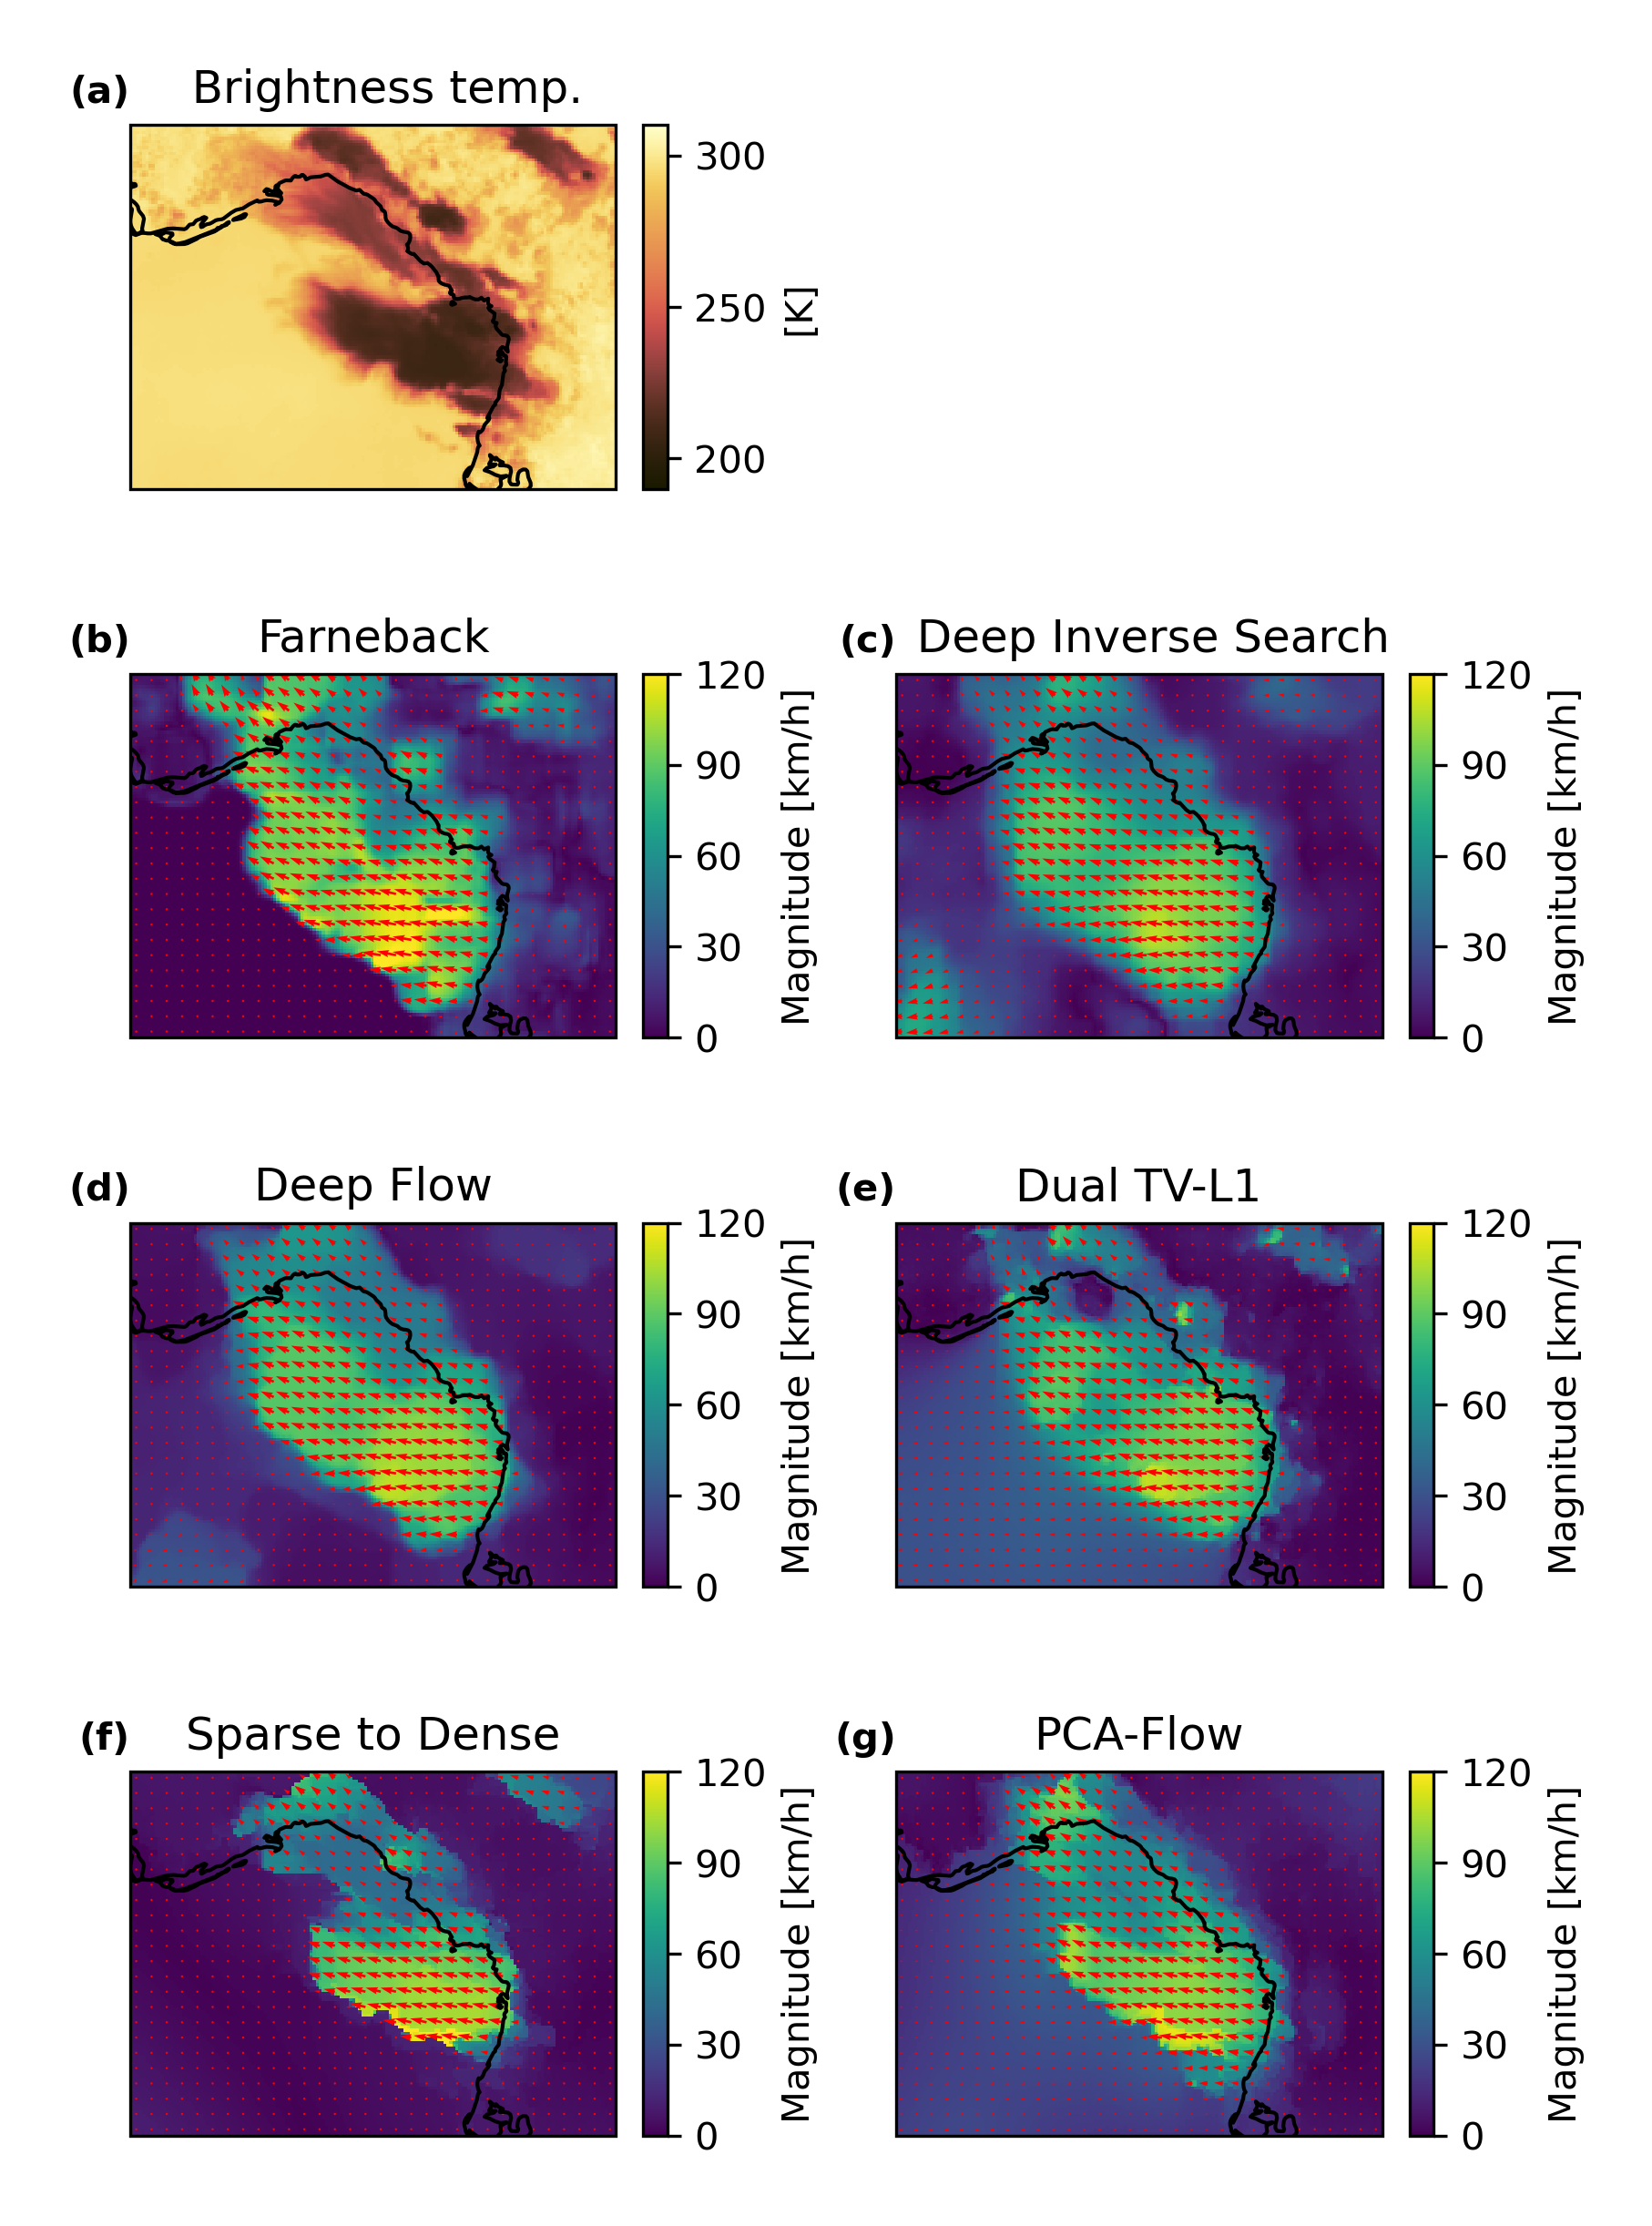
\includegraphics[width=0.9\textwidth]{figures/chapter1_10.png}
    \caption[
    A comparison of the motion vector fields generated by different optical flow methods
    ]{
    A comparison of the motion vector fields generated by the (b) Farnebäck, (c) \acrshort{dis}, (d) DeepFlow, (e) \acrshort{dualtvl1}, (f) Sparse to Dense, and (g) \acrshort{pca}-Flow. Optical flow vectors shown are estimated between the 10.4\,\unit{\mu m} channel at 19:00:00 \acrshort{utc} (a) and the subsequent image. Red arrows (b--g) show the motion vectors averaged over each 5\texttimes 5-pixel area is plotted by the red arrows, and the background shows the magnitude of the velocity vectors.
    }
    \label{fig:opt_flow_comparison}
\end{figure}

\begin{figure}[t]
    \centering
    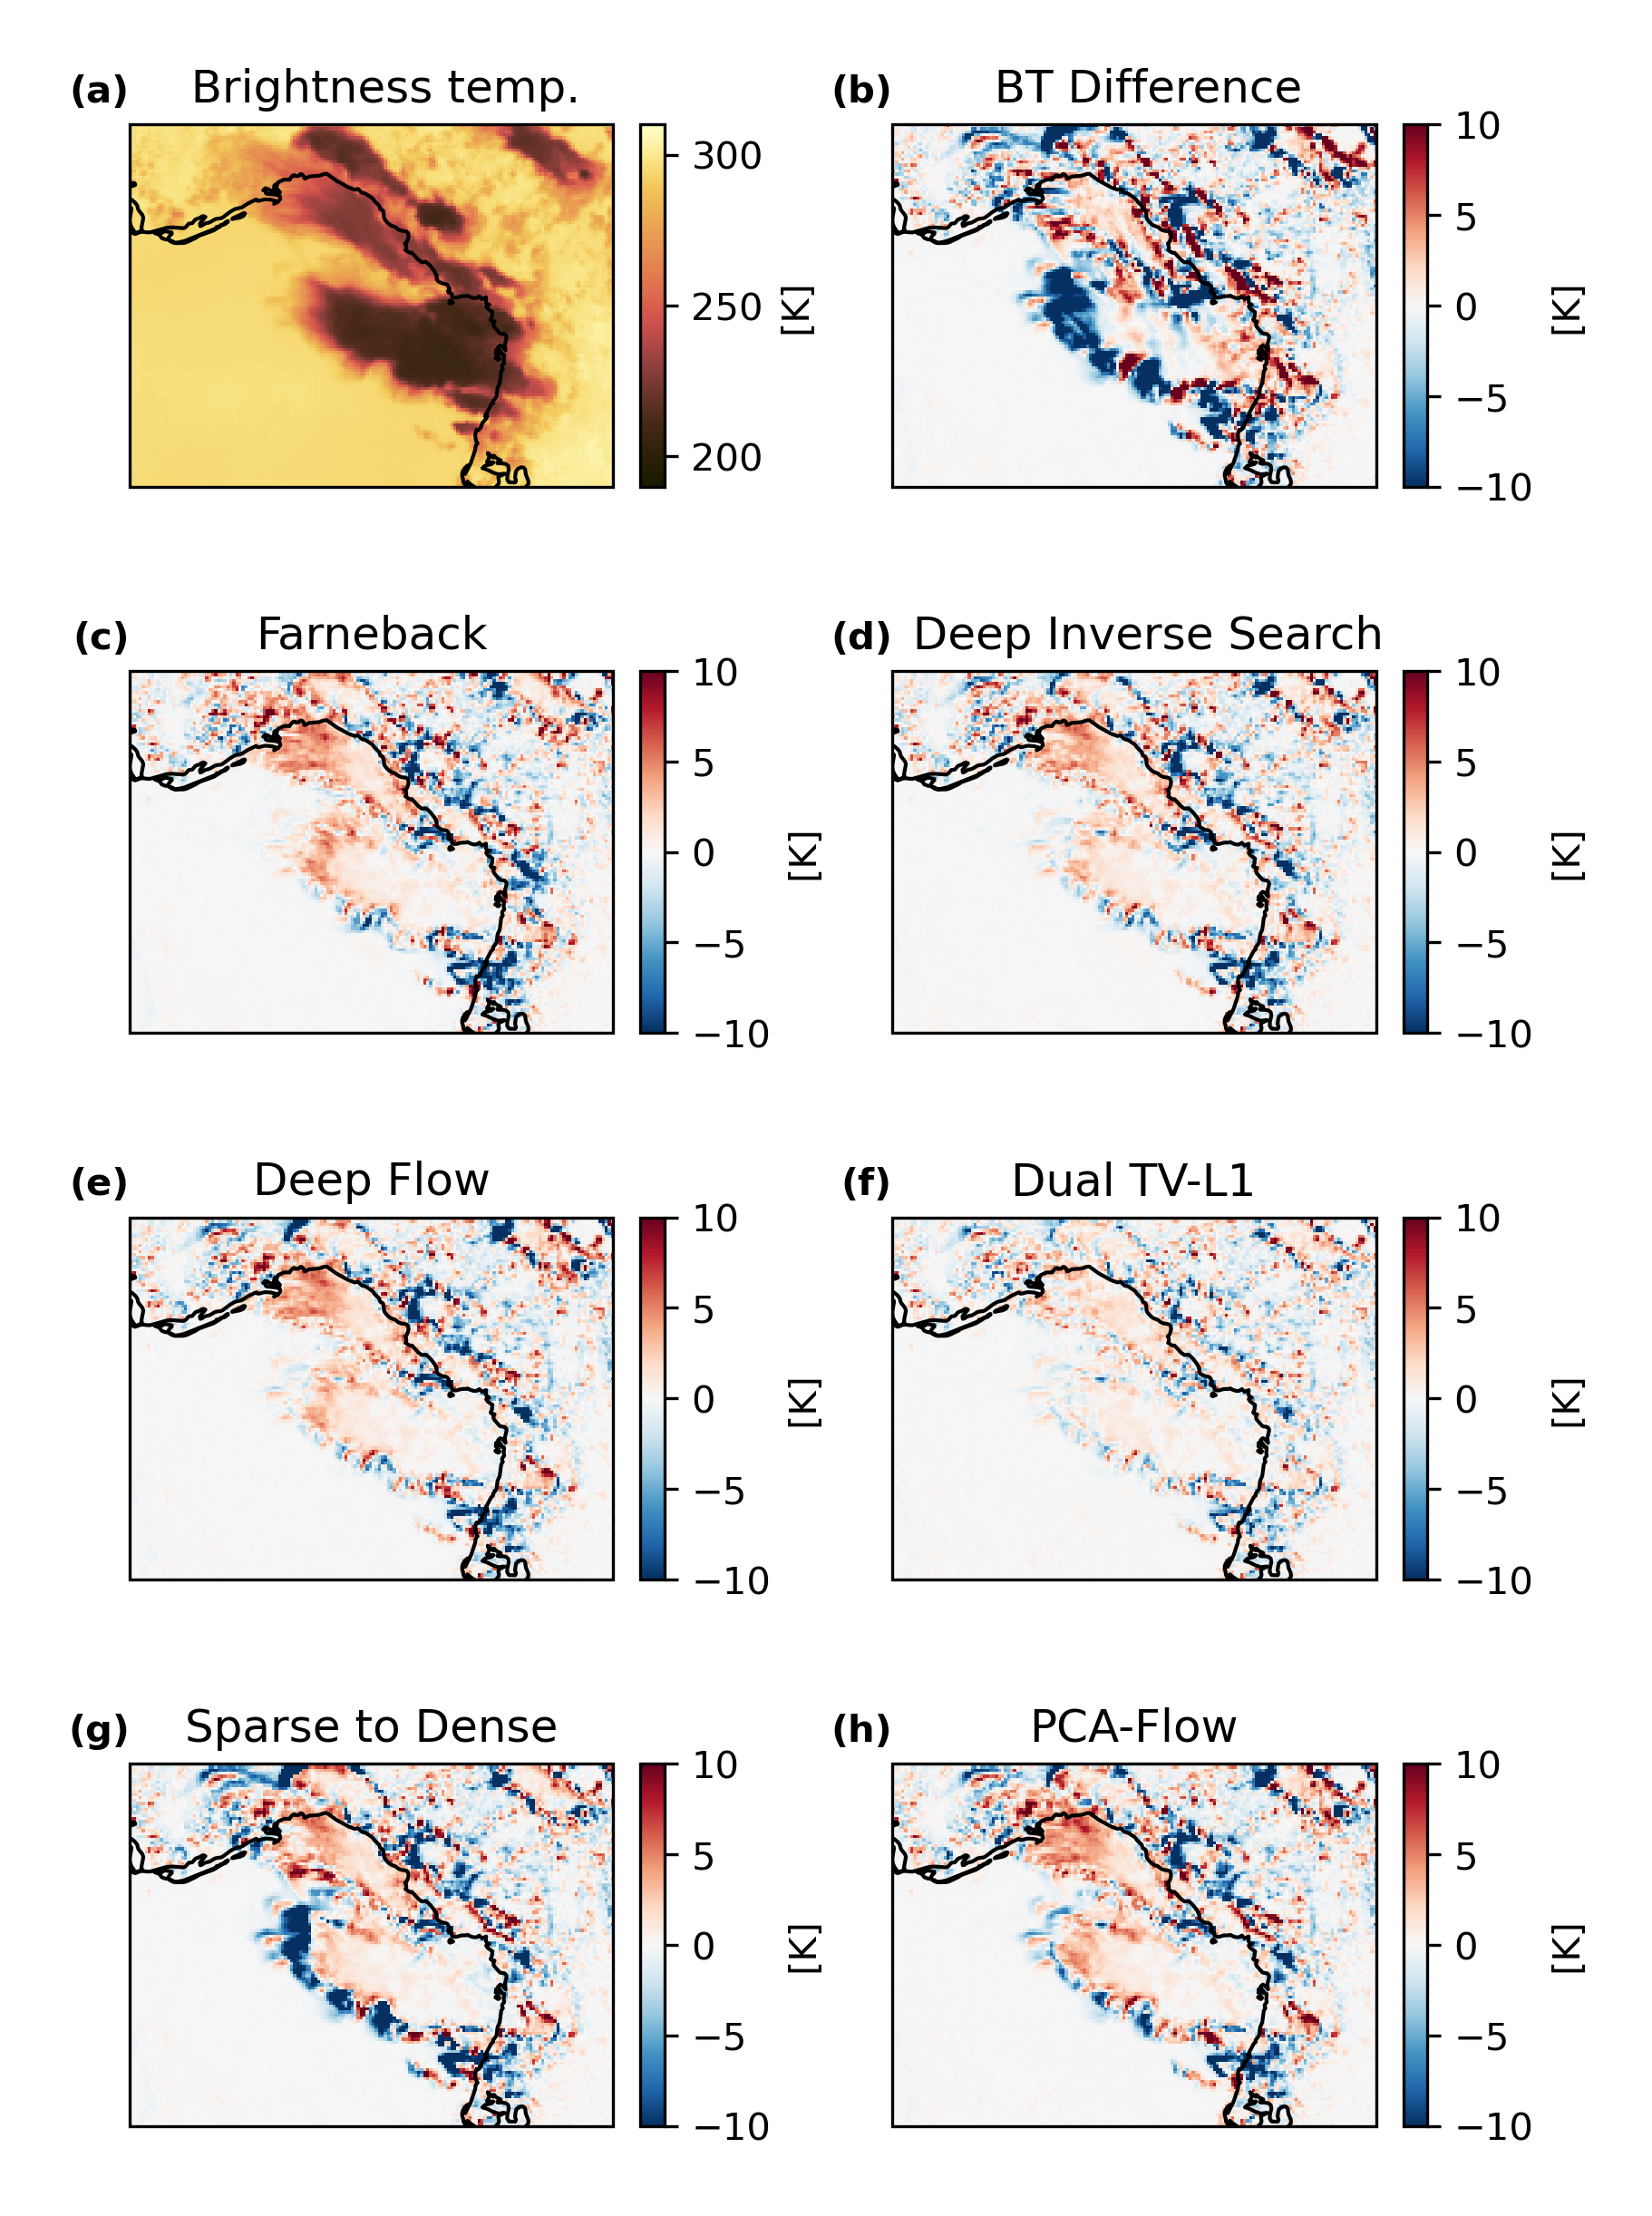
\includegraphics[width=0.9\textwidth]{figures/chapter1_11.png}
    \caption[
    The difference in \acrshort{bt} between subsequent \acrshort{abi} observations when taking into account the cloud motion predicted by the different optical flow algorithms.
    ]{
    The difference in \acrshort{bt} between subsequent \acrshort{abi} observations when taking into account the cloud motion predicted by the different optical flow algorithms. The plots are again shown for the time step at 19:00:00~\acrshort{utc}, with the 10.4\,\unit{\mu m} \acrshort{bt} at this time step shown for reference (a). b: the Eulerian difference in \acrshort{bt}; c--h: the Lagrangian difference in \acrshort{bt} using motion vectors predicted by each of the optical flow algorithms.
    }
    \label{fig:opt_flow_differences}
\end{figure}

\begin{figure}[t]
    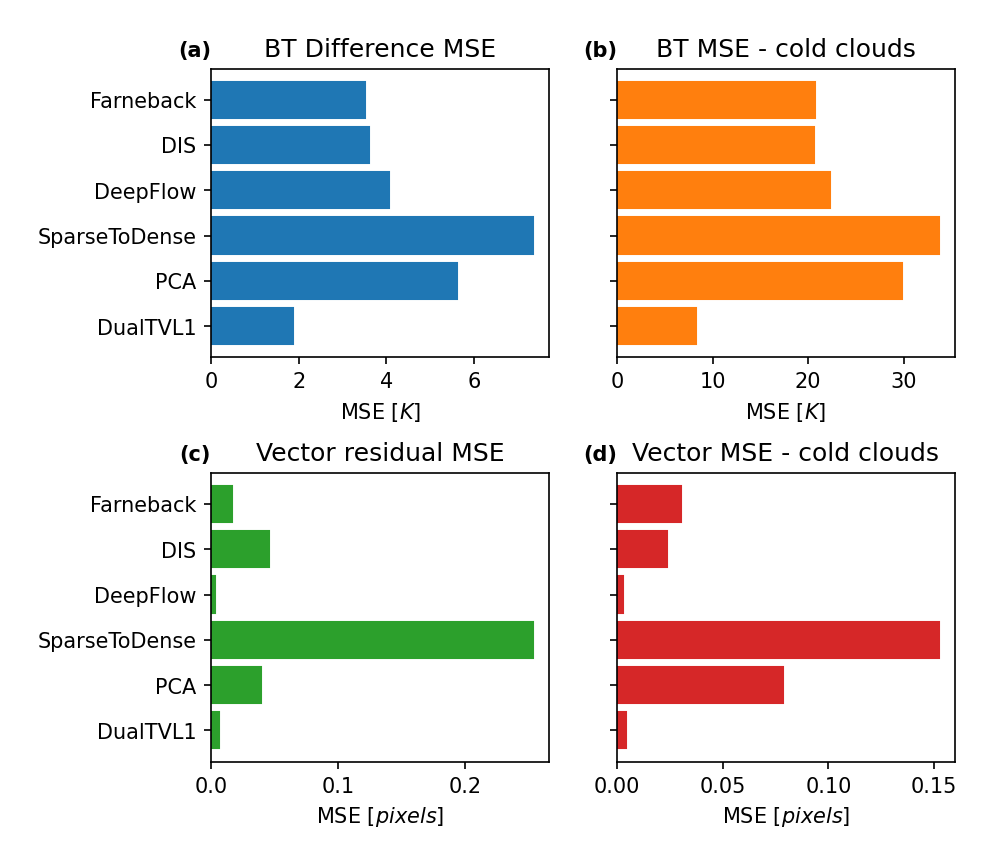
\includegraphics[width=\textwidth]{figures/chapter1_12.png}
    \caption[
    A comparison of the \acrshort{bt} difference and residual vector magnitude \acrshort{mse} for each of the optical flow algorithms
    ]{
    A comparison of the \acrshort{mse} for each of the optical flow algorithms. a: \acrshort{bt} difference \acrshort{mse} for all pixels and (b) for pixels with \acrshort{bt} $<$ 273\,\unit{K}. c: \acrshort{mse} of the residual vector magnitude for all pixels and (d) for pixels with \acrshort{bt} $<$ 273\,\unit{K}.
    }
    \label{fig:opt_flow_mse}
\end{figure}

\begin{figure}[t]
    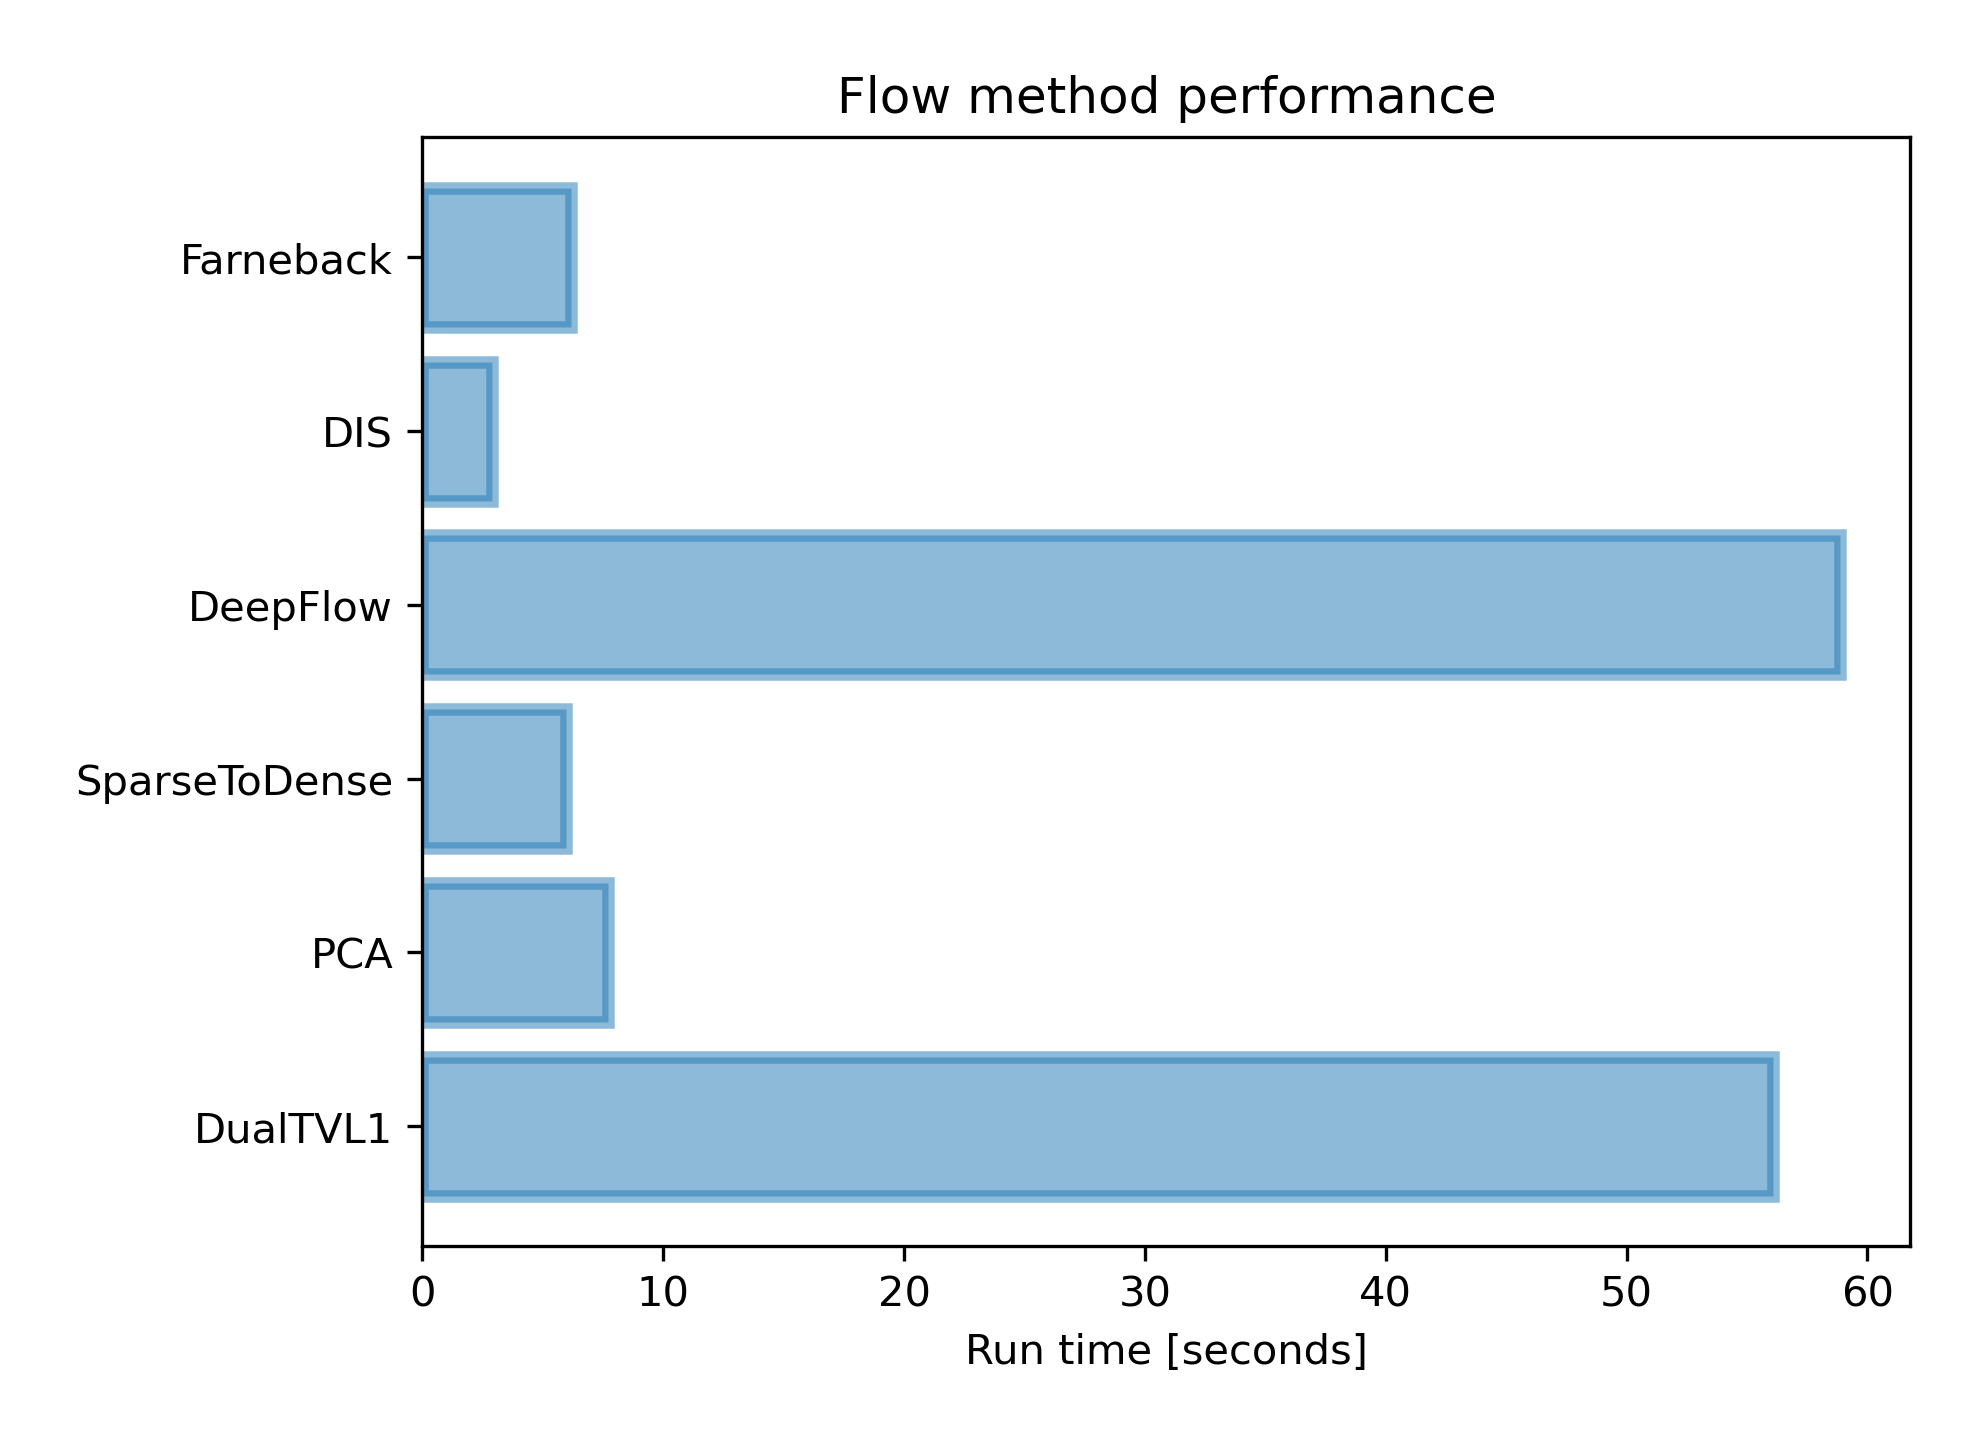
\includegraphics[width=\textwidth]{figures/chapter1_13.png}
    \caption[
    A comparison of the computational performance of each optical flow method
    ]{
    A comparison of the computational performance of each optical flow method. Run-time was measured for a sequence of 48 300\texttimes300 pixel \acrshort{abi} 10.4\,\unit{\mu m} \acrshort{bt} images.
    }
    \label{fig:opt_flow_cost}
\end{figure}


%f
\begin{figure}[t]
    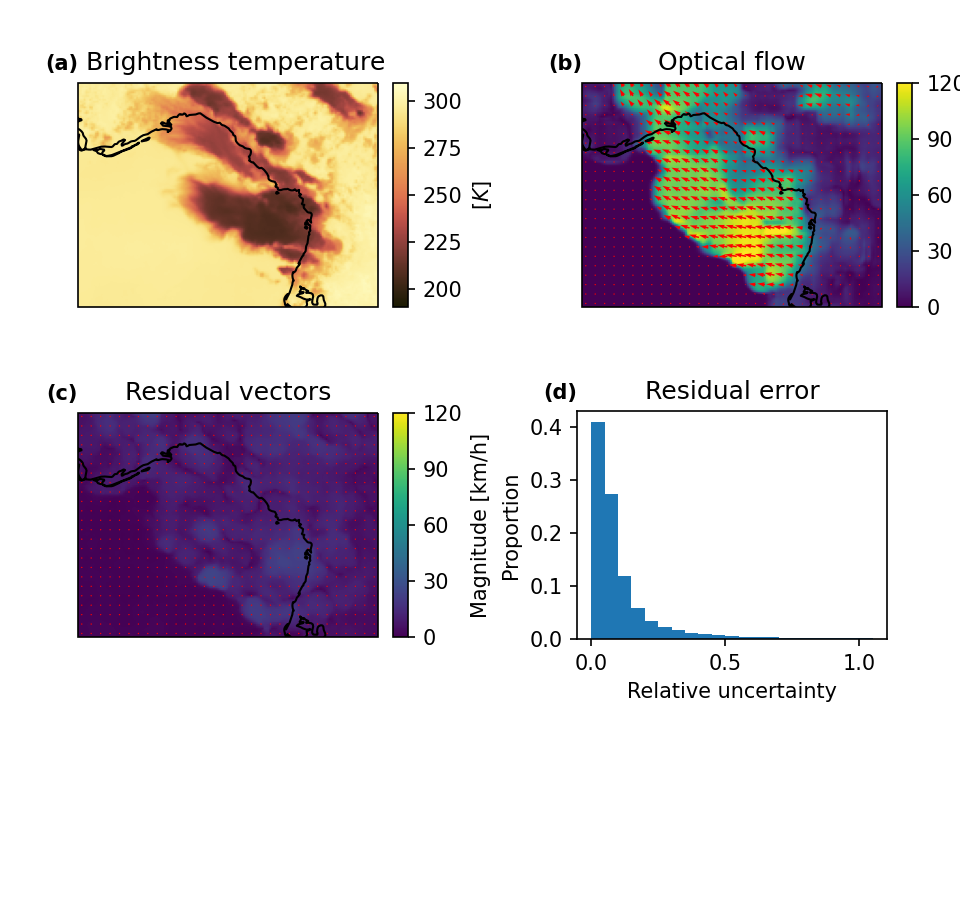
\includegraphics[width=\textwidth]{figures/chapter1_14.png}
    \caption[
    Relative residual error for optical flow motion vectors generated using the Farnebäck method
    ]{
    
    }
    \label{fig:optical_flow}
\end{figure}


The retrieval of \acrshort{amv}s has been performed since the earliest geostationary satellite observations \citep{menzel_cloud_2001}.
\acrshort{amv}s provide information about the motion of clouds in the atmosphere, including \acrshort{dcc}s \citep{bedka_application_2005}, and are routinely generated for the majority of operational geostationary earth observation satellites, including \acrshort{goes}-16 \citep{daniels_algorithm_nodate}. 
However, although \acrshort{amv}s may provide useful information about the motion of \acrshort{dcc}s, the non-geostrophic nature of wind fields in these conditions may result in the \acrshort{amv}s being calculated inaccurately or rejected by quality control checks \citep{bedka_application_2005}.

Optical flow algorithms are a family of algorithms used to estimate the apparent motion of objects observed in a series of images \citep{aggarwal_computation_1988}. 
A wide range of optical flow algorithms exist, and these have been successfully applied to many computer vision applications. 
It should be noted that optical flow does not necessarily represent the physical motion of an object, but is instead an estimation of the relative motion between an object and the observer and additionally any change in the apparent object (including growing, shrinking or other warping of the object). 

Optical flow algorithms have been previously shown to be accurate for the prediction of \acrshort{amv}s using geostationary satellite images \citep{wu_deriving_2016}, as long as the observations are sufficiently frequent such that the motion of unique features between images is less than the length scale at which neighbouring features can be resolved \citep{bresky_feasibility_2006}.
\citet{heikenfeld_tobac_2019} found that at imaging frequencies of less than 5~minutes the motion of \acrshort{dcc} cores was less than the spacing between neighbouring cores in the majority of cases, indicating that the frequency of the \acrshort{abi} \acrshort{conus} scan region is suitable for calculating optical flow vectors of \acrshort{dcc}s.
The use of optical flow has several advantages over traditional \acrshort{amv}s for the retrieval of \acrshort{dcc} motion vectors: optical flow can be calculated quickly using only two subsequent images and no \textit{a priori} information, aiding in near real-time applications; and also have no requirement for geostrophic balance. 
Optical flow algorithms are routinely used in the nowcasting of convective precipitation, and can be used to provide accurate predictions of \acrshort{dcc} with an hour of lead time using either radar or satellite observations \citep[e.g.][]{bowler_development_2004, bechini_enhanced_2017, woo_operational_2017}.
Optical flow, and similar motion vector techniques, have also been successfully applied to both the detection of developing deep convection \citep{zinner_cb-tram:_2008, zhang_locating_2014} and tracking detected deep convective features \citep{senf_size-resolved_2018} separately.

It should be noted that we are using optical flow to estimate the apparent motion of the cloud field between subsequent images, with the aim of using these vectors to map the locations of \acrshort{dcc}s from one step to the next, instead of calculating actual \acrshort{amv}s corresponding to winds.
This approach avoids a number of challenges with the use of optical flow for calculating \acrshort{amv}s including the estimation of the height of estimated flow vectors and the detection of diverging or converging motion vector fields in situations of growing and dissipating clouds respectively.
In the latter case, we in fact aim to include the divergence and convergence within the optical flow vector field to map both the location and shape of observed clouds between time steps.

\subsubsection{Evaluation of Optical Flow Methods}

As different optical flow algorithms may provide better accuracy in different situations \citep{baker_database_2011}, we compare a number of different algorithms to assess their suitability for tracking the motions of \acrshort{dcc}s.
We consider six different optical flow algorithms implemented in the OpenCV library \citep{opencv_library}, which are listed below:

\begin{itemize}
    \item Farnebäck \citep{farneback_two-frame_2003}
    \item \acrshort{dis} \citep{kroeger_fast_2016}
    \item DeepFlow \citep{weinzaepfel_deepflow_2013}
    \item \acrshort{dualtvl1} \citep{zach_duality_2007, perez_tv-l1_2013}
    \item Sparse to Dense \citep{bouguet_pyramidal_1999}
    \item \acrshort{pca}-Flow \citep{wulff_efficient_2015}
\end{itemize}

The first four of these algorithms are dense optical flow methods, which calculate motion vectors for every pixel in the image.
The final two calculate sparse optical flow---motion vectors between detected objects in each image, rather than individual pixels---and then map these to all pixels based on a region segmentation approach.
The sparse to dense and \acrshort{pca}-flow algorithms use the Lucas-Kanade method \citep{lucas_iterative_1981} and the \acrshort{pca} method respectively to calculate the sparse motion vectors.

Each algorithm was applied to a sequence of images from the 10.4\,\unit{\mu m} channel, with the algorithms estimating motion vectors between each consecutive pair of images.
As the methods require 8-bit images, a linear normalisation was applied to the \acrshort{bt} images between each pair's minimum and maximum values.
To improve the accuracy of the detected motion vectors, a variational refinement process \citep{brox_high_2004} is applied to the calculated flow vectors.
This process minimises the energy functional of the pixel value, pixel gradient, and local smoothness to reduce the angular error of the detected flow vectors.
Finally, vectors are calculated both forwards and backward in time between each pair of images, and these two sets of vectors are interpolated to each others locations and averaged to ensure that they are equal and opposite.

Figure~\ref{fig:opt_flow_comparison} shows the \acrshort{abi} \acrshort{bt} at 19:00:00~\acrshort{utc} (fig.~\ref{fig:opt_flow_comparison}\,a), along with the optical flow vectors calculated by each of the algorithms with the subsequent time step.
For each set of optical flow vectors, the average vector over each 5\texttimes 5-pixel area is plotted by the red arrows, and the vector velocity magnitude is plotted in the background.
The two sparse methods (fig.~\ref{fig:opt_flow_comparison}\,f,g) show a closer match of the areas where optical flow vectors to the edge of the anvil cloud than the dense methods (fig.~\ref{fig:opt_flow_comparison}\,b--e), which have a tendency to smooth the detected vectors over a large area.
Of all the methods, the Farnebäck algorithm tends to produce larger magnitudes, but correctly detects zero flow in areas without clouds, unlike most of the algorithms.

Figure~\ref{fig:opt_flow_differences} shows the difference in \acrshort{bt} between subsequent observations when taking into account the cloud motion predicted by the different optical flow algorithms.
The plots are again shown for the time step at 19:00:00~\acrshort{utc}, with the 10.4\,\unit{\mu m} \acrshort{bt} at this time step shown again for reference in fig.~\ref{fig:opt_flow_differences}\,a.
Figure~\ref{fig:opt_flow_differences}\,b shows the Eulerian difference in \acrshort{bt}; the difference in the \acrshort{bt} observed at the same pixel locations on subsequent time steps.
We see large cooling rates of the left (downwind) side of the anvil cloud, not because the \acrshort{ctt} is cooling, but because of the expansion of the anvil cloud into previously cloud-free areas.
Removing these erroneous observations of cloud-top cooling caused by the motion and expansion of the anvil cloud is the main objective of the semi-Lagrangian approach.

The dense optical flow methods (fig.~\ref{fig:opt_flow_differences}\,c--f) show good performance in removing the anomalous cooling observations seen downwind of the anvil cloud.
The Farnebäck, \acrshort{dis} and DeepFlow algorithms (fig.~\ref{fig:opt_flow_differences}\,c--e) all show a warming tendency towards the edge of the anvil cloud.
Although this may be explained by an overestimation of the cloud motion by these algorithms, this may also be a real observation of apparent warming due to thinning of the detraining anvil cloud.
The \acrshort{dualtvl1} algorithm (fig.~\ref{fig:opt_flow_differences}\,f) shows generally smaller differences than the other algorithms.
This is likely due to the algorithm accounting for changes in brightness between observations, whereas the other algorithms assume that the brightness of tracked objects remains constant between observations.

The two sparse optical flow algorithms (fig.~\ref{fig:opt_flow_differences}\,g,h) both show worse performance, with the sparse to dense method performing particularly poorly.
Both algorithms show cooling downwind of the anvil, likely because the region-based methods used to map the sparse motion vectors to the whole image do not detect this region well.

Figure~\ref{fig:opt_flow_mse}\,a shows the \acrshort{mse} of the \acrshort{bt} differences shown in fig.~\ref{fig:opt_flow_differences} for each algorithm.
As seen in fig.~\ref{fig:opt_flow_differences}, the \acrshort{dualtvl1} algorithm has the smallest differences, the other dense algorithms perform similarly, and the \acrshort{pca}-Flow and sparse to dense algorithms perform the worst.
It should be noted that we should expect some differences in the \acrshort{bt} due to actual changes in the \acrshort{ctt}.
Figure~\ref{fig:opt_flow_mse}\,b shows the \acrshort{mse} of the \acrshort{bt} differences for pixels with \acrshort{bt} less than 273\,\unit{K}, representing cold cloud observations.

To estimate the uncertainty in the calculated motion vectors, we calculate the residual motion vectors for each algorithm.
The residual motion is calculated by first warping each image to the locations predicted by the optical flow vectors, in the same manner used to calculate the \acrshort{bt} differences in fig.~\ref{fig:opt_flow_differences}.
Then the optical flow algorithms are used to calculate a second set of residual vectors between each image and the subsequent warped image.
In theory, if the initial motion vectors were calculated perfectly, warping the image by the optical flow vectors should result in the subsequent cloud in the same position as the prior image, and so the second set of motion vectors should calculate as zero.
The magnitude of the residual motion vectors is therefore considered as the uncertainty in the initial set of motion vectors.

Figure~\ref{fig:opt_flow_mse}\,c,d show the \acrshort{mse} of the residual vector magnitudes for all pixels and pixels less than 273\,\unit{K} respectively.
The DeepFlow and \acrshort{dualtvl1} algorithms again show the best accuracy, and sparse to dense the worst.
The Farnebäck algorithm shows good accuracy across all pixels, as seen in the ability to correctly detect zero motion in cloudless skies in fig.~\ref{fig:opt_flow_comparison}.
However, when considering only cold pixels the Farnebäck algorithm performs slightly worse than \acrshort{dis}.

The results shown in fig.~\ref{fig:opt_flow_mse} suggest that the \acrshort{dualtvl1} algorithm is the best choice for estimating the motion vectors in satellite observations of \acrshort{dcc}.
However, due to the large size and long sequences of images produced by \acrshort{abi}, it is also important to consider the computational cost of each algorithm.
Figure~\ref{fig:opt_flow_cost} shows the run time in seconds for each algorithm applied to a sequence of 48 300\texttimes300~pixel \acrshort{abi} \acrshort{bt} images.
Both the DeepFlow and \acrshort{dualtvl1} algorithms show significantly longer run times than any of the other algorithms.
As a result, we have selected the Farnebäck algorithm for out tracking method as it offers the best balance of accuracy and computational performance for running on large datasets.

An example of the motion vectors calculated by the Farnebäck algorithm when applied to the 10.4\,\unit{\mu m} \acrshort{bt} field is shown in fig.~\ref{fig:optical_flow}.
Figure~\ref{fig:optical_flow}\,c shows the residual flow vectors, which are small compared to the detected cloud motion vectors (fig.~\ref{fig:optical_flow}).
The main areas in which residual flow vectors can be seen are the regions around the edge of anvil clouds and in the center of thick anvil clouds where there are no clear features to track.
Figure~\ref{fig:optical_flow}\,d shows the distribution of residual vector errors proportional to the detected cloud motion vectors.
The majority of the residual errors are close to zero, and very few exceed 0.5.
As in the majority of applications for the semi-Lagrangian we are only interested in the motion to the nearest pixel, these errors are acceptable.

Two potential sources of uncertainty are the assumptions made by the Farnebäck algorithm that the feature being tracked remains the same size and intensity in subsequent images.
For optical flow tracking using \acrshort{bt} images of growing \acrshort{dcc}s, neither of these assumptions are true.
However, we have taken steps to reduce the impact of both these sources of uncertainty on the tracking algorithm.
For the first of these assumptions, we find that in the case of small, fast-moving \acrshort{dcc}s -- where the accuracy of the optical flow vectors is most important -- the changes in the size of the \acrshort{dcc} is small compared to the overall motion, and so the uncertainty introduced is small.
Comparably, for large \acrshort{dcc}s where the changes in size may be large compared to the motion, the uncertainty introduces has less impact on the tracking algorithm.
In the worst-case scenario, the estimated optical flow field will be zero, in which case the "3D" detection and tracking algorithm works in the same manner as that of \citet{fiolleau_algorithm_2013}, which is suitable for use on these larger \acrshort{dcc}s.

\subsection{A Semi-Lagrangian Framework for Morphological Image Processing}

Morphological image operations analyse images using their geometrical and structural properties.
Core to many morphological algorithms, from simple filters to complex neural networks \citep{kalchbrenner_convolutional_2014}, is the kernel, or convolution method.
A convolution method performs operations on the pixels of an image by applying a convolution stencil to the pixel and its neighbours.
In a conventional convolution scheme, such as that used in the methods of \citet{fiolleau_algorithm_2013}, the convolution stencil acts on adjacent pixels in both time and space (see fig.~\ref{fig:convolution_kernels}\,a).
In this Eulerian framework, different locations in time are considered in the same manner as those in the spatial dimensions.
However, we know from previous analysis of \acrshort{dcc}s that the motion of convective cores between images can be similar to the spacing of cores and their size \citep{heikenfeld_tobac_2019}.
As a result, it is important to include the effects of advection when comparing images across time steps.


%f
\begin{figure}[t]
    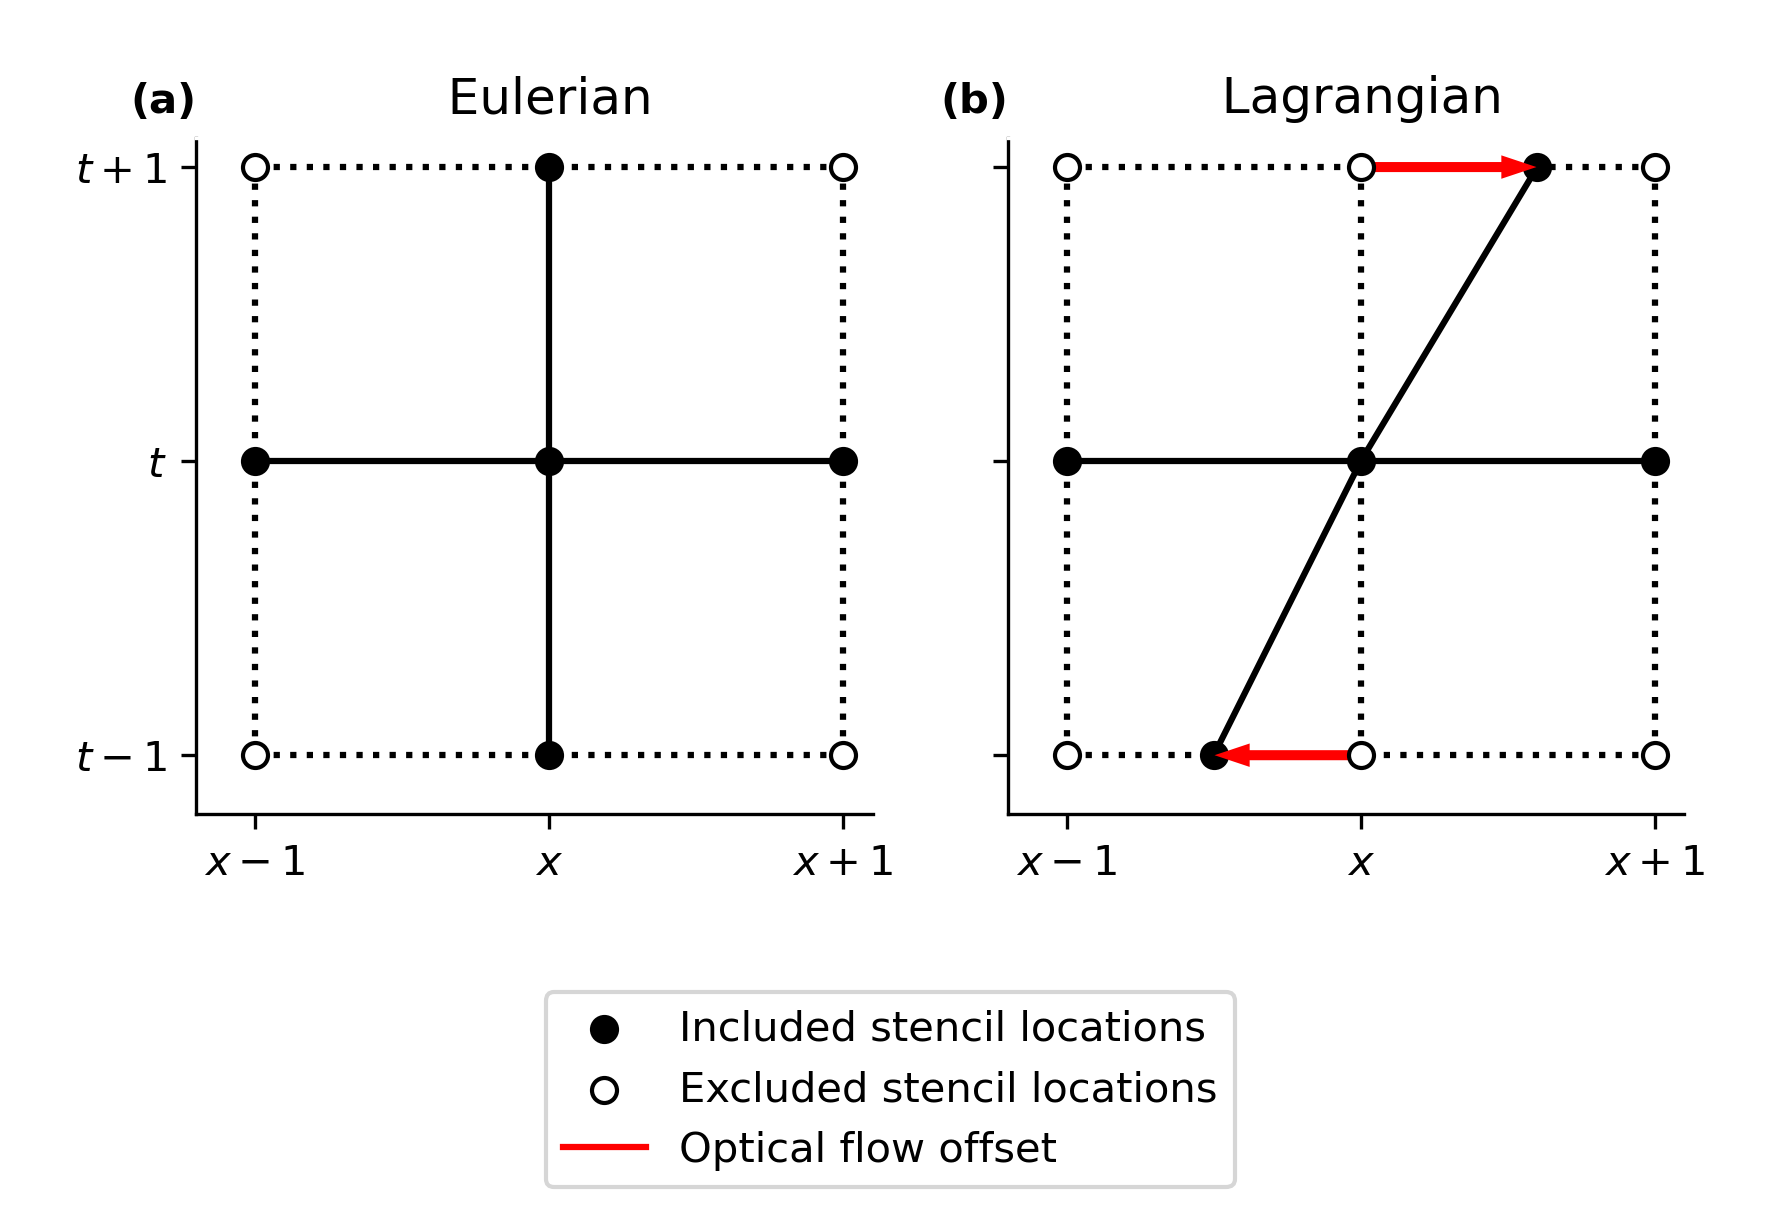
\includegraphics[width=\textwidth]{figures/chapter1_15.png}
    \caption[
    A comparison of convolution stencils with square connectivity in Eulerian and Lagrangian frameworks.
    ]{
    A comparison of convolution stencils with square connectivity in Eulerian (a) and Lagrangian (b) frameworks. In the Lagrangian framework, the points at prior and subsequent time steps are offset by the calculated optical flow field.
    }
    \label{fig:convolution_kernels}
\end{figure}


To perform morphological operations which take into account this advection, we have developed a novel Lagrangian convolution method.
For spatial operations, the Lagrangian stencil operates identically to that of a classical convolution method.
However, when sampling points at prior or subsequent time steps, the location of the stencil are offset by the relevant optical flow vectors (fig.~\ref{fig:convolution_kernels}\,b).
Values at the offset stencil locations are interpolated, providing a Lagrangian reference frame for changes in the observations over time.
When applying the convolution stencil to every pixel in a sequence of images, this provides a semi-Lagrangian framework for morphological operations, combining the Lagrangian reference frame for evaluating changes over time while maintaining the regular grid of the images.

We have developed new implementations of several existing image processing operations within the Lagrangian convolution framework, including:
\begin{itemize}
    \item Sobel edge detection \citep{sobel_isotropic_2014}
    \item Watershed segmentation using the connected-components method \citep{bieniek_efficient_2000}
    \item Labelling of connected components \citep{hoshen_percolation_1976}
\end{itemize}

These operations are used in this method to detect the full extent of the anvil cloud associated with the \acrshort{dcc}, to perform detection continuously across multiple time periods while accounting for the motion of the \acrshort{dcc}, and to identify individual \acrshort{dcc}s and \acrshort{dcc} clusters across multiple time periods respectively.

The Sobel method detects edges in an image using the magnitude of the local gradient at each pixel.
Edge detection enables the segmentation of an image into separate regions without pre-defined thresholds (such as in \acrshort{bt}) to separate them.

Watershed algorithms are a method of image segmentation that equate an image to a topographical map, with elevation according to the value of the pixel.
Each pixel is then descended towards its local minima until it reaches a predefined marker region.
The method takes its name from the geographical feature of the same name, which refers to the separation between adjacent drainage basins.
Although this physical interpretation of the algorithm applies to two-dimensional images, the method can be applied to arrays with any number of dimensions, such as the method used by \citet{fiolleau_algorithm_2013} which applied watershedding to a three-dimensional field.

Labelling algorithms assign unique identifiers to each segmented region provided by either the edge detection or watershed algorithms.

\subsection{Detection of Growing Deep Convection}

%f
\begin{figure}[t]
    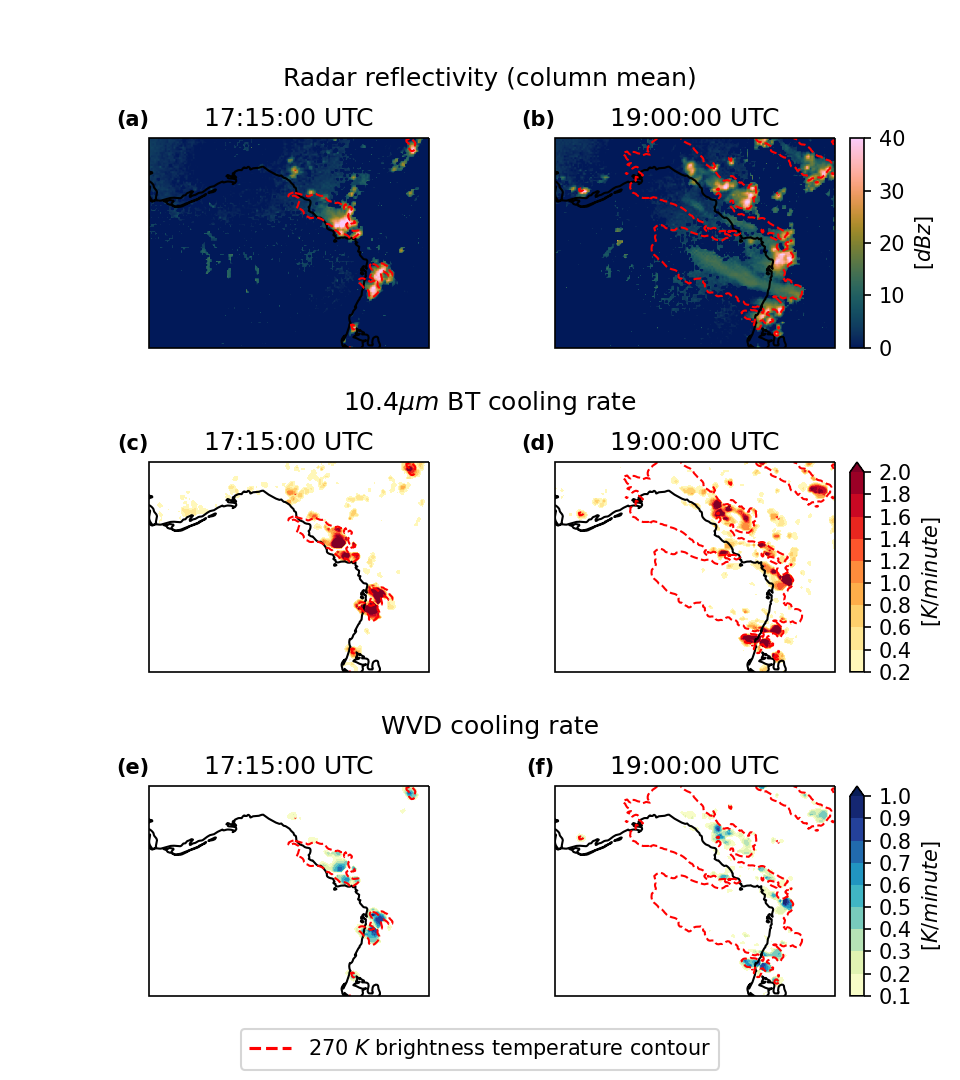
\includegraphics[width=\textwidth]{figures/chapter1_16.png}
    \caption[
    Detection of growing \acrshort{dcc} regions for the \acrshort{dcc} cluster in figure~\ref{fig:compare_sat_radar_glm}
    ]{
    Detection of growing \acrshort{dcc} regions for the \acrshort{dcc} cluster in figure~\ref{fig:compare_sat_radar_glm}. 15 minute average cooling rate in the \acrshort{goes}-16 \acrshort{abi} \acrshort{wvd} field is used to detect growing cores. This is effective in the growing phases of convection (a.), but becomes less effective during the mature phase (b.). Comparison with \acrshort{nexrad} column mean radar reflectivity remapped to the \acrshort{abi} grid(c., d.). An average cooling rate of greater than 0.5\,\unit{K min\textsuperscript{-1}} is indicative of a growing convective core.
    }
    \label{fig:core_detection}
\end{figure}

Growing deep convective cores are detected in a similar manner to that used by \citet{zinner_cb-tram:_2008}.
The growth rates are calculated using the finite difference of the 10.4\,\unit{\mu m } \acrshort{bt} and \acrshort{wvd} fields in the Lagrangian perspective.
We have found that combining both the 10.4\,\unit{\mu m} \acrshort{bt} and the \acrshort{wvd} field provides the best observations for detecting growing deep convective cores.
The \acrshort{bt} field shows cooling cloud tops throughout the troposphere, while the \acrshort{wvd} isolates growth in the mid- to upper-troposphere, removing spurious observations of growth due to boundary layer convection and cloud formation.

We classify a region of growing deep convection as a region of either continuous cooling of greater than 0.5\,\unit{K} per minute in the 10.4\,\unit{\mu m} \acrshort{bt} field, or continuous warming of the \acrshort{wvd} field of at least 0.25\,\unit{K} per minute.
These growth rates must be detected over a minimum 15-minute period, covering an area of at least 3 by 3 pixels (approximately 7.5 by 7.5\,\unit{km}) at each time step.
Each region of detected growth is given a unique label, the average \acrshort{bt} of the detected cloud at each time step is calculated, and any label which fail to meet the cooling rate thresholds of 8\,\unit{K} over a 15-minute period (from \citep{roberts_nowcasting_2003, hartung_intercomparison_2013}) are removed.
Finally, each label is checked to ensure that the growth region ends with a \acrshort{wvd} field with a value of greater than -5, indicating that the growing core reaches a high altitude \citep{muller_role_2018}.

Figure~\ref{fig:core_detection} shows a comparison between the detected core cooling rates in \acrshort{abi} imagery and the corresponding column radar reflectivity measured by \acrshort{nexrad} for the case of newly developing convection (fig.~\ref{fig:core_detection}\,a,c,e) and mature \acrshort{dcc} (fig.~\ref{fig:core_detection}\,b,d,f)
Both 10.4\,\unit{\mu m} \acrshort{bt} and \acrshort{wvd} growth rates show growth detected in the same locations as the high column radar reflectivity from \acrshort{nexrad}.

However, during the mature stage of the \acrshort{dcc}, discrepancies develop between the observed cooling rate (fig.\ref{fig:core_detection}\,b) and the radar reflectivity (fig.~\ref{fig:core_detection}\,d) due to the development of the anvil cloud blocking satellite observations of the core underneath.

\subsection{Detection of Anvil Clouds}

%f
\begin{figure}[t]
    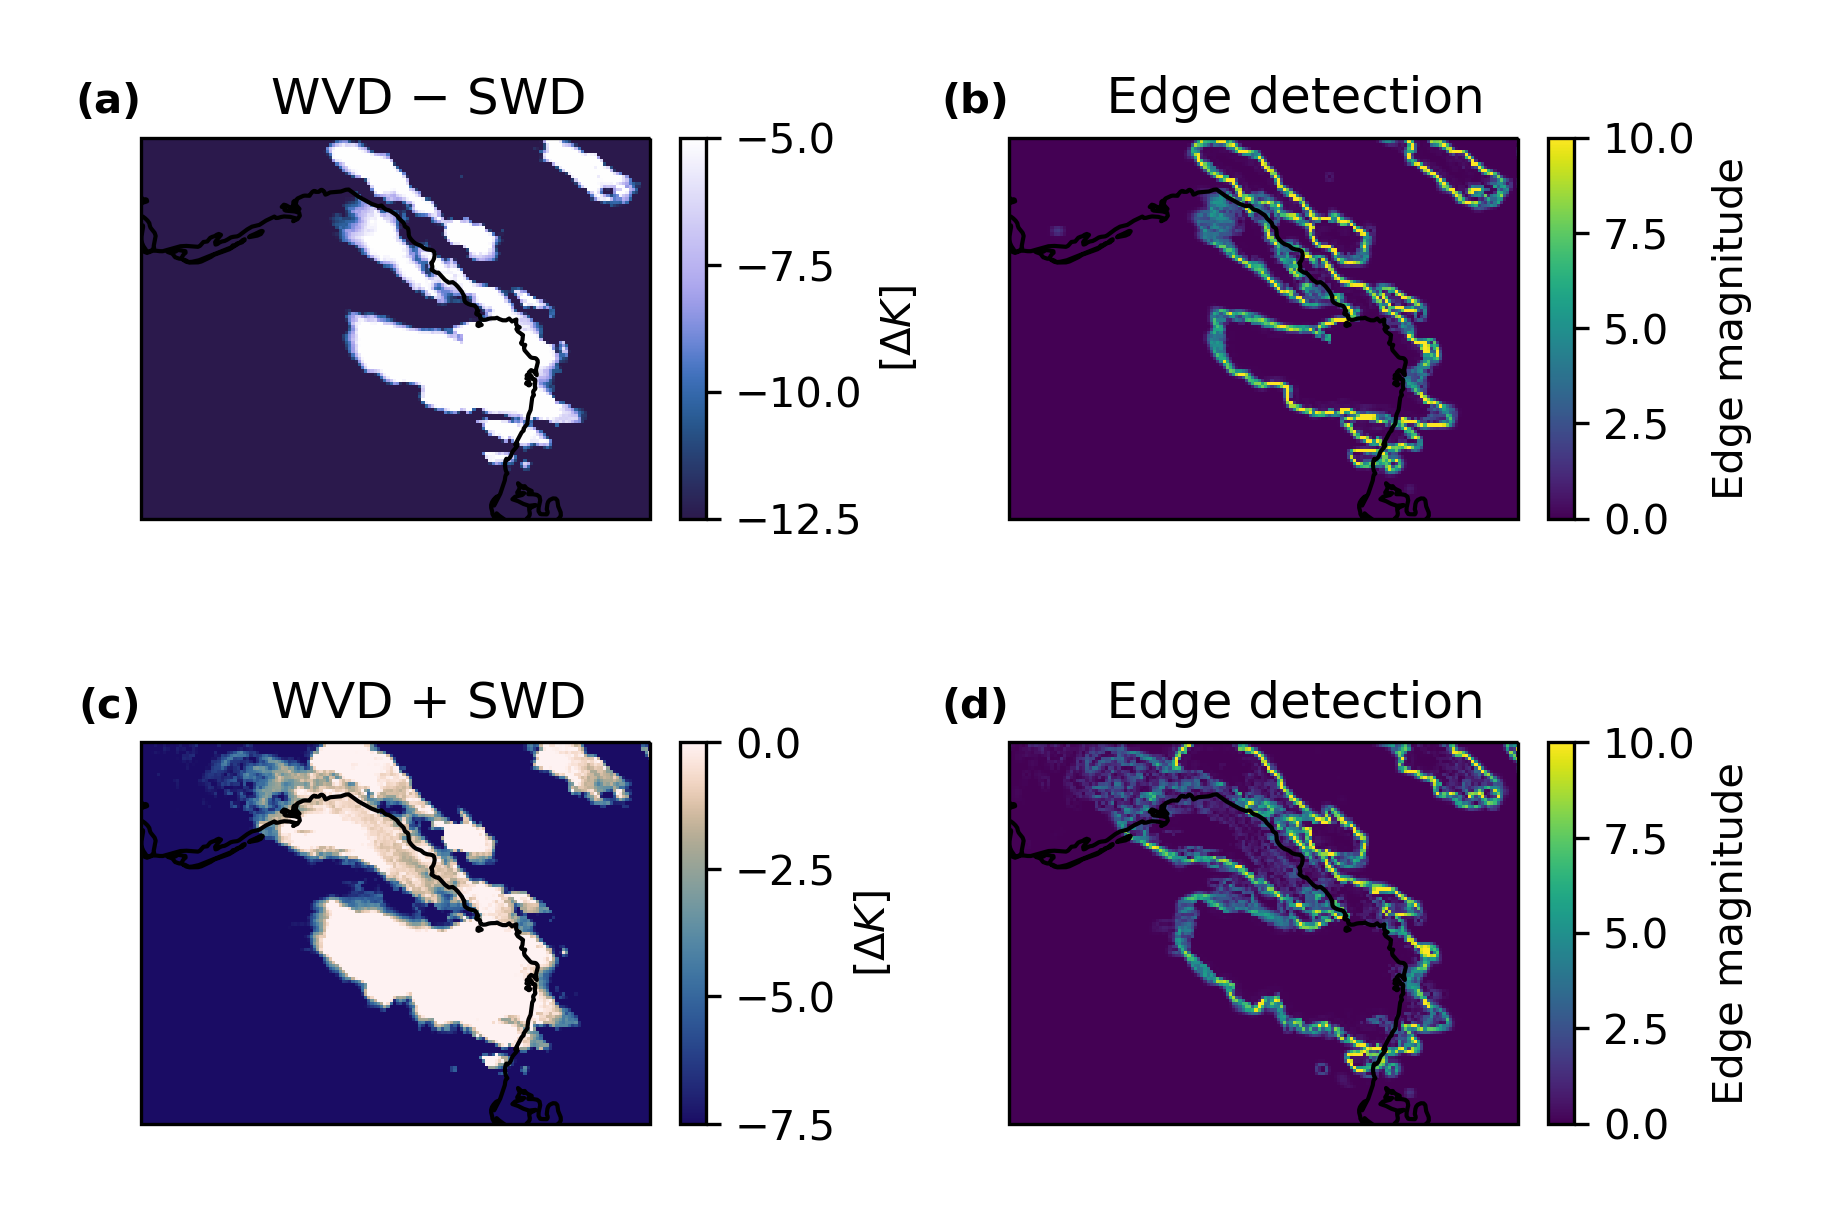
\includegraphics[width=\textwidth]{figures/chapter1_17.png}
    \caption[
    Detection of anvil cloud extent for the mature \acrshort{dcc} cluster in \ref{fig:compare_sat_radar_glm} using the edge gradient method
    ]{
    Detection of anvil cloud extent for the mature \acrshort{dcc} cluster in \ref{fig:compare_sat_radar_glm} using the edge gradient method. a.: The combined field of the \acrshort{wvd} minus the \acrshort{swd}, to isolate the thick anvil, between the upper and lower thresholds of -5 and -12.5\,\unit{K} respectively. b.: the detected edge gradient magnitude of the field between these thresholds, which is used to detect the outer extent of the thick anvil cloud. c.: the combined field of \acrshort{wvd} plus the \acrshort{swd}, to enhance the thin anvil, and d.: the calculated edge magnitude of this field.
    }
    \label{fig:edge_detection}
\end{figure}

%f
\begin{figure}[t]
    \centering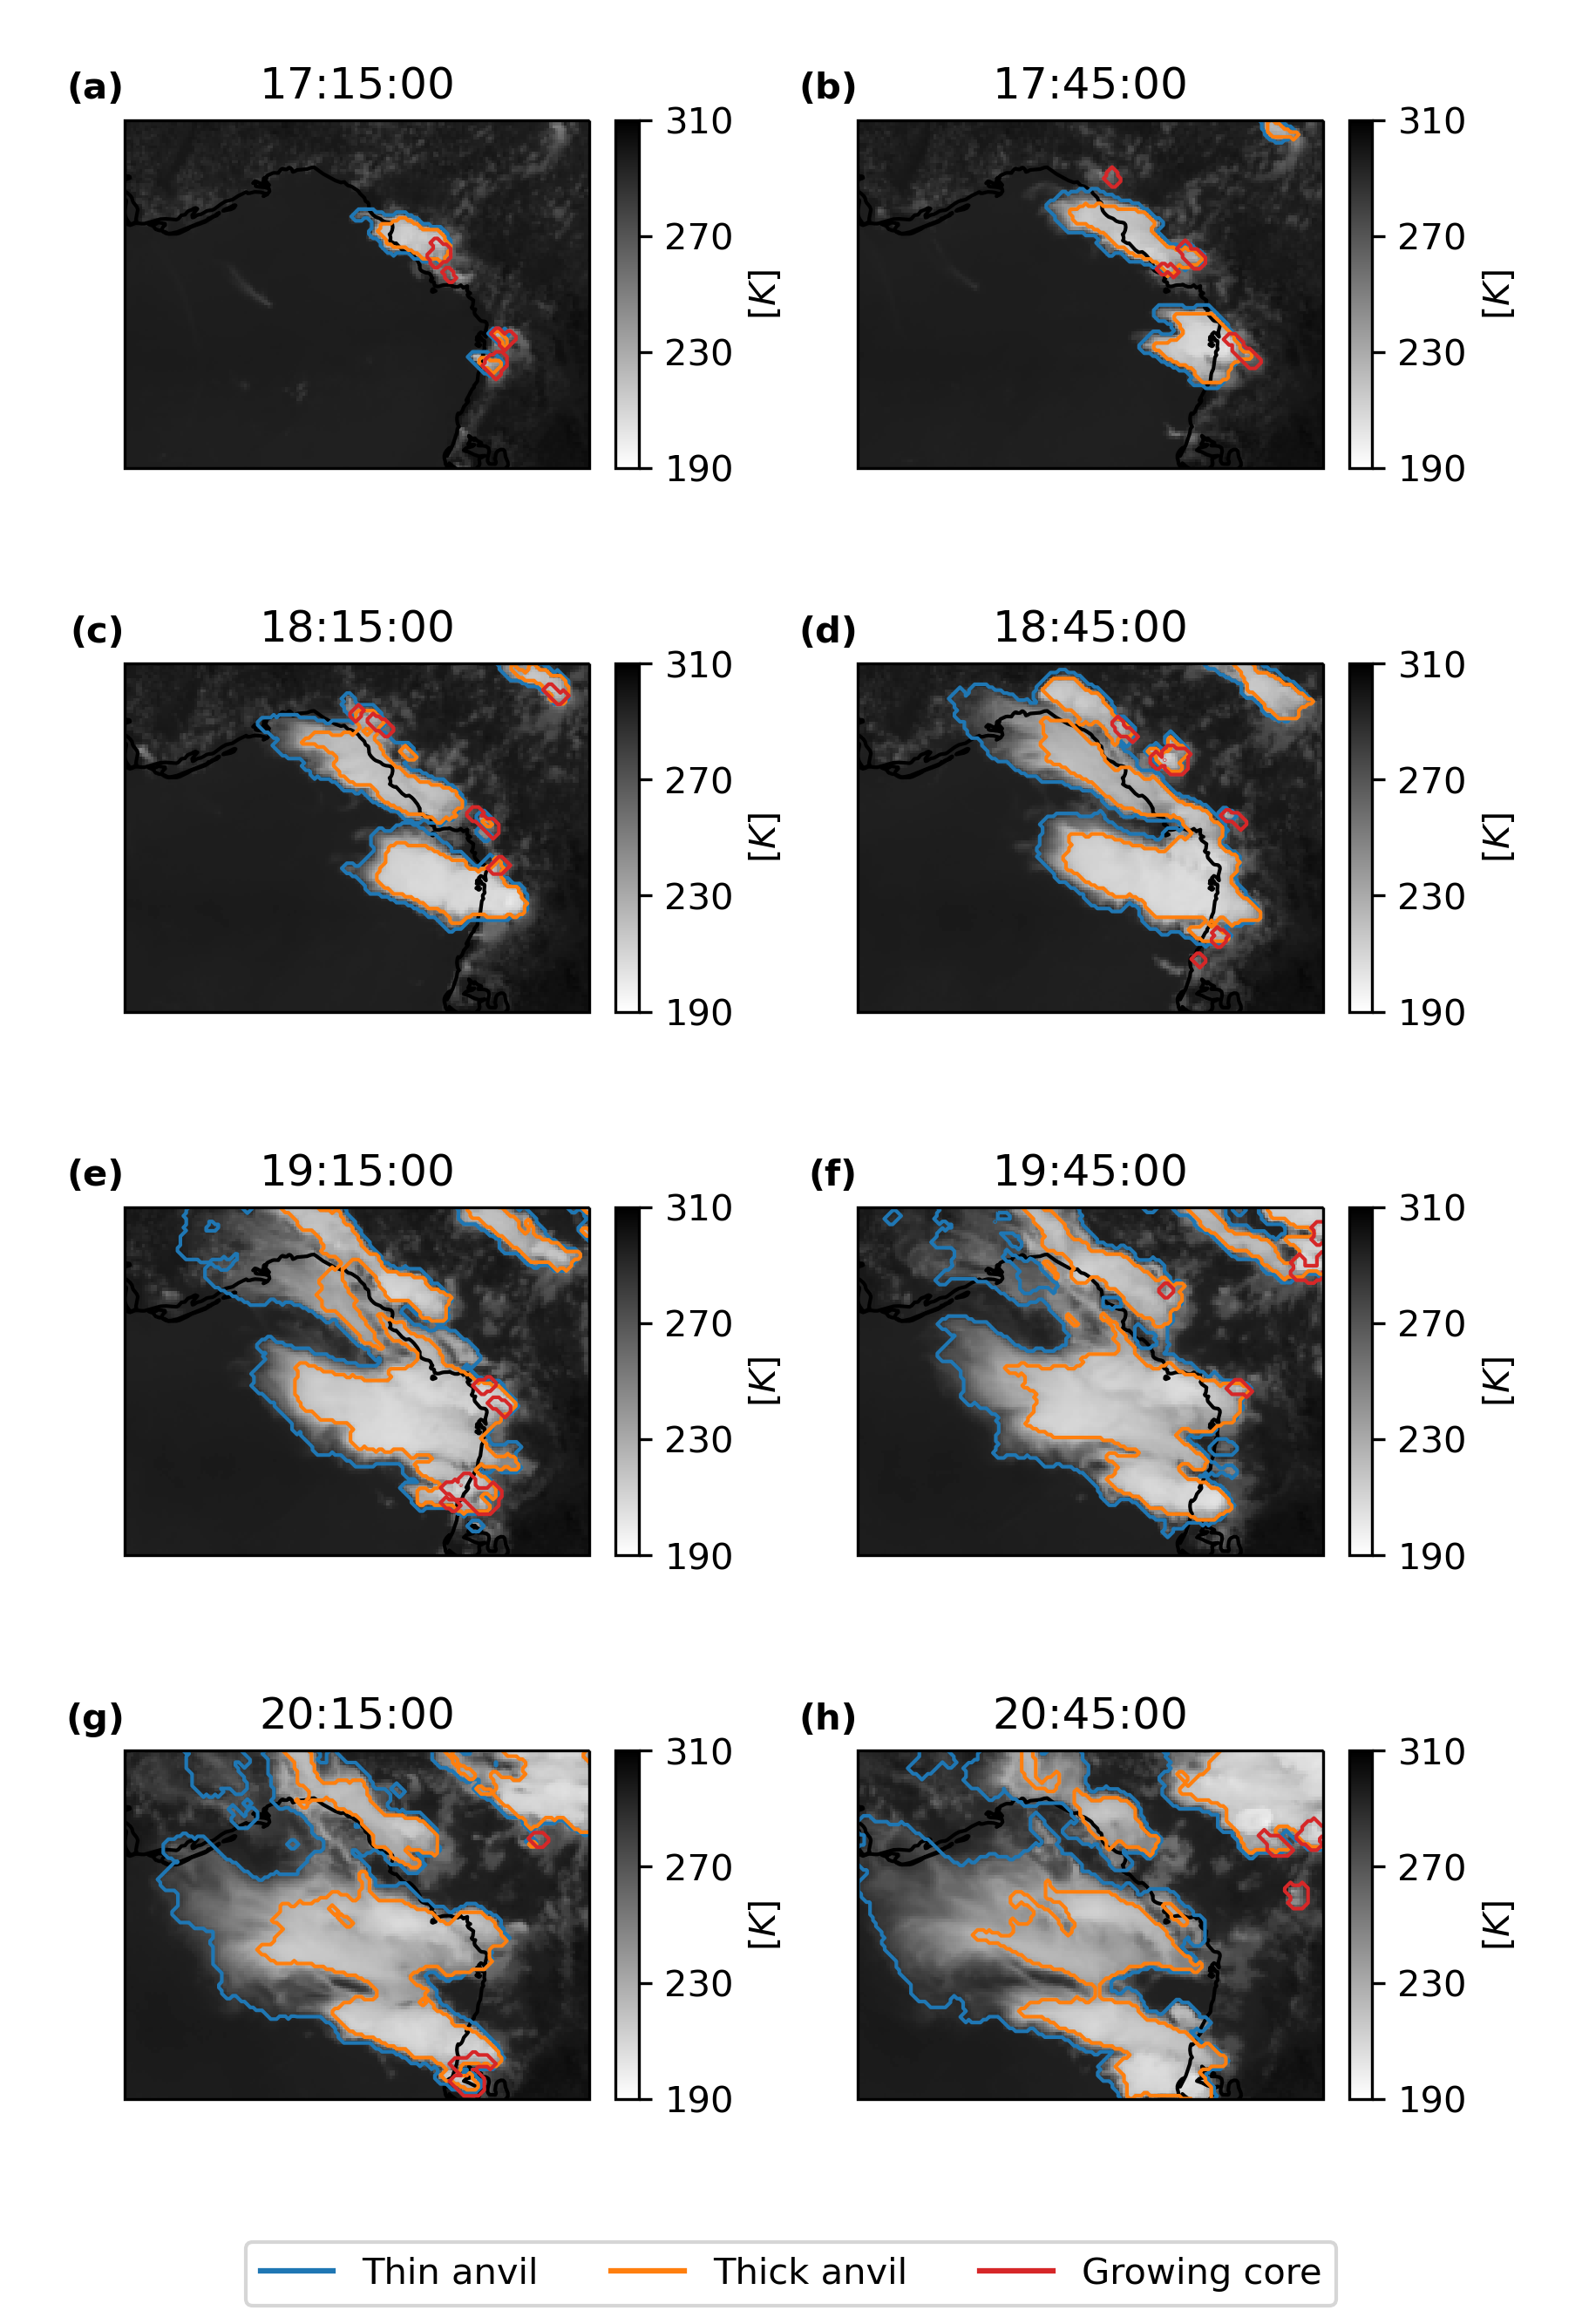
\includegraphics[width=0.8\textwidth]{figures/chapter1_18.png}
    \caption[
    Detected regions of thin anvil cloud (blue), thick anvil cloud (orange), and developing cores (red) overlaid on the \acrshort{goes}-16 \acrshort{abi} 10.4\,\unit{\mu m} \acrshort{bt} field for the \acrshort{dcc} cluster from figure~\ref{fig:compare_sat_radar_glm}
    ]{
    Detected regions of thin anvil cloud (blue), thick anvil cloud (orange), and developing cores (red) overlaid on the \acrshort{goes}-16 \acrshort{abi} 10.4\,\unit{\mu m} \acrshort{bt} field for the \acrshort{dcc} cluster from figure~\ref{fig:compare_sat_radar_glm}. The three stages of the \acrshort{dcc} lifecycle are shown; the growth phase (a.), the mature phase (b.), and the dissipating phase (c.). Note that the anvil region continues to be detected in c. after growing cores are no longer detected.
    }
    \label{fig:detected_anvils}
\end{figure}

The region of anvil cloud associated with the growing convective clouds detected in the previous section is detected and tracked using an edge-based watershed segmentation approach.
The edge-based approach to cloud detection avoids the use of a fixed threshold for anvil temperature, and so can detect a more accurate extent of the anvil cloud \citep{dim_alternative_2013}.
We define an upper threshold for the \acrshort{wvd} field of -5\,\unit{K}, as used by \citet{muller_role_2018}, and a lower threshold of -12.5\,\unit{K}, which we define as definite non-anvil cloud.
Because the presence of thin cirrus outflow from the anvil clouds can make it difficult to determine the extent of the anvil cloud, we use the \acrshort{swd} field as described in section 2.1 to either remove or include the region of cirrus outflow in the detected anvil region.
To detect the thick anvil cloud, we subtract the \acrshort{swd} field (fig.~\ref{fig:edge_detection}\,a).
In this case, the upper and lower thresholds remain the same as the \acrshort{swd} field is approximately 0~K for thick, high clouds, and so has no effect on the temperature of these features.
For detecting the thin anvil region, we add the \acrshort{swd} field and increase the value of both thresholds by 5\,\unit{K} to 0\,\unit{K} and -7.5\,\unit{K} respectively (fig.~\ref{fig:edge_detection}\,c).
This change is made to account for the effect of low-level \acrshort{wv} on the \acrshort{swd} field which gives a background value of approximately 5~K.
Between these two thresholds, we have a region in which we are uncertain of the extent of the anvil cloud.
By applying a Sobel filter to detect the local gradient magnitude of the combined \acrshort{wvd}/\acrshort{swd} field \citep{sobel_isotropic_2014}, we detect the outer extent of the anvil cloud within this region where we see the greatest magnitude in the detected edges (see fig.~\ref{fig:edge_detection}\,b,d).
%(fig.~\ref{fig:edge_detection}b).

When applied to the detected edges of the anvil clouds using the Sobel filter, with the growth regions detected previously as markers, the watershed method allows us to detect those anvil regions associated with detected regions of growing \acrshort{dcc}s, while avoiding the detection of non-convective regions of high, cold clouds.
Furthermore, due to the application of the watershed algorithm to both the spatial and temporal dimensions of the sequence of images through the semi-Lagrangian framework, we are able to detect the associated anvil clouds after the growth of the \acrshort{dcc} is no longer observed (see fig.~\ref{fig:detected_anvils}).

Figure~\ref{fig:detected_anvils} shows an example of the results of detecting and tracking \acrshort{dcc} cores and their associated anvils.
Detection of the cores (outlined in red) and the initial development of the associated anvils (outlined in orange and blue for the thick and thin anvil regions respectively) can be seen in fig.~\ref{fig:detected_anvils}\,a.
In fig.~\ref{fig:detected_anvils}\,b we see the development of the mature anvil, which primarily consists of thick anvil, and secondary core detections as new convection develops at the edge of the \acrshort{dcc}.
In fig.~\ref{fig:detected_anvils}\,c, we see the detected anvil cloud beginning to dissipate, and a larger proportion of the anvil cloud detected as thin anvil.
At this point in the lifetime of the tracked \acrshort{dcc} we no longer observe any growing core, however the "3D" approach allows the continued tracking of the anvil cloud until it dissipates.

% To detect the regions of \acrshort{dcc} and their associated anvils from the observations of growing cores outlined in the previous section, a watershedding approach over both space and time is applied in a similar to that used by Fiolleau and Roca [cite].
% Watershed algorithms are a class of techniques commonly used for image segmentation.
% Watershed algorithms work by emulating the behaviour of a geographical watershed.
% Each location in the input array is assigned to a `basin' surrounding a local minima.
% If these basins overlap a set of supplied markers, all the locations in the basin are assigned to the image segment of those markers.
% The remaining basins are then flooded until they overflow into a neighbouring basin.
% The basin is then either assigned to the same segment of the image as the neighbouring basement, or, if both are unassigned, the two basins are merged and the process repeated until all basins are assigned to segments of the image.
% There are a wide range of implementations of watershedding algorithms, however it should be noted that despite the class usually being referred to in reference to the segmentation of images, these techniques can be applied to data with any number of dimensions.

% A network based watershedding algorithm has been implemented here, albeit with the addition of a semi-Lagrangian treatment of the temporal dimension.
% Most watershedding algorithms only consider the connectivity of pixels with their nearest neighbours in each dimension when assigning basins.
% The algorithm used by Fiolleau in Roca used this approach for both the spatial and temporal dimensions, however, as highlighted by Heikenfeld [cite], the distance travelled by individual convective cells between the images provided by geostationary satellites may be significant in relation to separation of individual cells.
% As a result, only considering pixels at the same location in the temporal dimension may result in either missed detections for small, rapidly advecting cores, or in extreme cases the false connection of cores due to their advection causing their locations to overlap in subsequent images.
% Here, instead of treating the temporal dimension with an Eulerian approach (taking the same locations in adjacent time frames to be neighbours), the selection of neighbouring pixels in the temporal dimension is instead offset by the observed cloud motion using the optical flow vectors.
% This allows both the continuous detection of small, moving \acrshort{dcc}s, but also the ability to distinguish closely spaced \acrshort{dcc}s.
% Furthermore, it is expected that this will allow the detection algorithm to be applied to datasets with coarser time resolution, however this has not yet been tested.

% To avoid the use of a fixed threshold for the detection of \acrshort{dcc}s, an edge detection based approach is used for the watershedding of detected \acrshort{dcc}s, which is demonstrated in fig.~\ref{fig:watershed}.
% Rather than selecting a fixed threshold for the masking of convective and non-convective clouds, with the associated uncertainties as discussed prior, a region of `uncertainty' is selected.
% This region is chosen as all pixels where the \acrshort{wvd} is between -5~K (the same threshold as used by muller et al), and -15~K, below which the cloud is assumed to be non-convective.
% Within the uncertain region, the magnitude of the local gradients of the field are calculated using a Sobel filter (as used by Dim and Takamura [cite]), and the calculated Sobel gradients used as an input for the watershed algorithm.
% When observing a cloud field, the maximum gradient is expected to be observed at the edge of the cloud, allowing the entire volume of the anvil cloud to be detected regardless of the specific temperature of the cloud field.
% To further enhance the ability to distinguish individual clouds using the edge detection method, a variety of channel combinations are utilised to show greater contrast between \acrshort{dcc}s and the surrounding environment.
% Firstly, for the detection of thick anvil clouds, the \acrshort{swd} is subtracted from the \acrshort{wvd}, removing the influence of thin cirrus outflow from the cloud field as this may make the edges of the cloud appear indistinct.
% By instead adding the \acrshort{swd} to the \acrshort{wvd}, it is possible to both enhance the observation of thin cirrus outflow and enhance the contrast between it and the surrounding cloud field.
% This second field allows us to detect a larger area encompassing both the thick convective core and anvil cloud, and the associated cirrus outflow, and allows further investigation into changes in the behaviour of anvil clouds to a variety of environmental conditions.

\section{Evaluation}

% %f
% \begin{figure}[t]
%     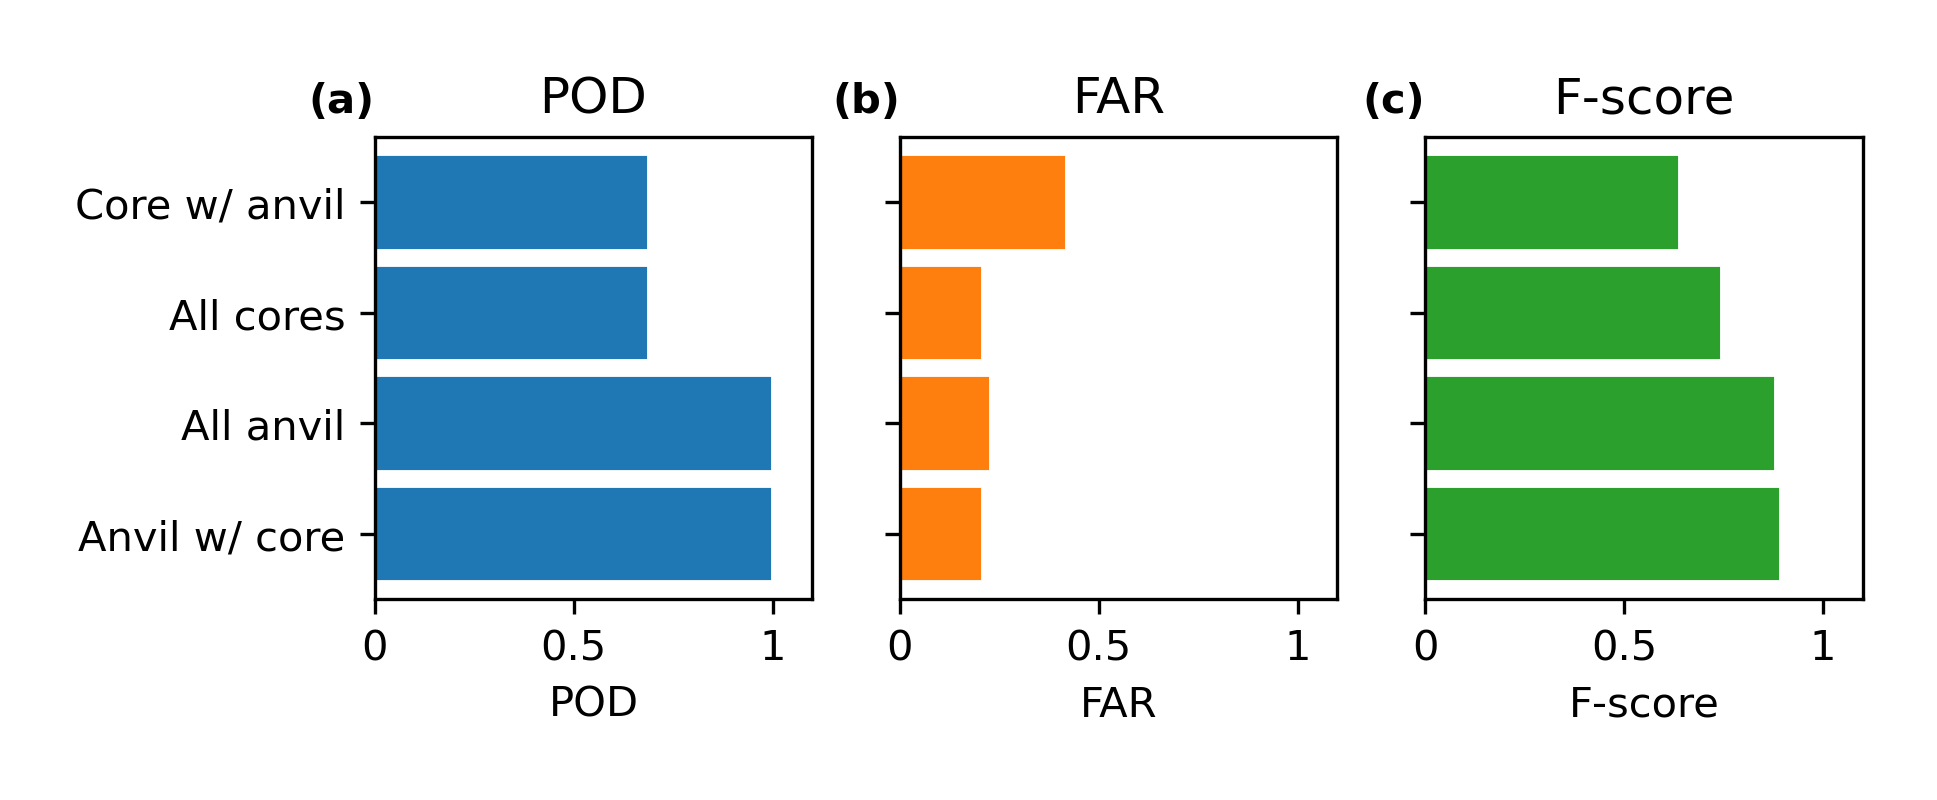
\includegraphics[width=\textwidth]{figures/chapter1_19.png}
%     \caption[
%     \acrshort{pod}, \acrshort{far} and F-score for detected core and anvil regions evaluated against \acrshort{glm} lightning observations
%     ]{
    
%     }
%     \label{fig:validation}
% \end{figure}


The effectiveness of the semi-Lagrangian framework for the detection of \acrshort{dcc}s is evaluated by analysing the proximity of detected anvil cloud regions to lightning flash detection from \acrshort{glm}.
Lightning observations are frequently used to validate detection methods for deep convection \citep[e.g.][]{zinner_validation_2013, muller_novel_2019} due to the strong correlation between deep convective updraughts and lightning activity.
Although \acrshort{glm} is not capable of detecting all lightning events (approximately 70\% of lightning events are detected) \citep{peterson_removing_2020}, the high frequency of lightning flashes per \acrshort{dcc} mean that these observations provide a suitable ground truth for validation.
It should be noted that lightning observations are only suitable for validating the detection of the thick anvil region, as lightning does not occur in the cirrus outflow.
As a result, validation of the detection of the thin anvil region would require the use of other data such as cloud profiling radar or lidar observations, and is not considered further in this paper.
% not provide a perfect ground truth as it detects approximately 70\% of all lightning flashes within the field, and can also report false detections due to a number of causes.
% However, these uncertainties are considered insignificant for the validation of the detection of deep convection due to the large number of lightning flashes associated with individual deep cores, and improved data cleaning and flagging respectively.

Here we apply the same validation method as used by \citet{muller_novel_2019} to evaluate the semi-Lagrangian framework for the detection of \acrshort{dcc}s.
We classify detection events into three categories:

\begin{itemize}
    \item Correct detection (CD), when the algorithm detects a \acrshort{dcc} that is collocated with one or more lightning observations
    \item False detection (FD), when the algorithm detects a \acrshort{dcc} but no lightning flash is observed
    \item Missed detection (ND), when the algorithm does not detect a \acrshort{dcc} but a lightning flash is observed
\end{itemize}

Using these three categories of events we can define two measures of accuracy for the detection of \acrshort{dcc}s.
The \acrshort{pod} is defined as the number of correct detections divided by the total number of correct and missed detections.
This provides a measure of how likely the algorithm is to detect a \acrshort{dcc} that exists in the ground truth.
The \acrshort{far} is defined as the number of false detections divided by the total number of correct and false detections.
This provides a measure of how likely a \acrshort{dcc} detected by the algorithm is not present in the ground truth.

When evaluating whether detected \acrshort{dcc} regions and lightning observations were collocated \citet{muller_novel_2019} considered events within 32\,\unit{km} and 15 minutes to be collocated.
This margin of uncertainty was separated into two section, half from the physical separation between observed lightning strikes, and the remaining half from uncertainty in the collocation and geolocation of the satellite and lightning observations.
For a typical \acrshort{abi} pixel length over the \acrshort{conus} of 3\,\unit{km}, this margin of error translates into 10 pixels in the \acrshort{abi} view.
The distance between a \acrshort{glm} lightning flash and detected cloud region is defined as the distance between the flash and the nearest \acrshort{abi} pixel within that region, with \acrshort{glm} flashes that fall within a detected \acrshort{dcc} given a distance of 0.
When considering that the resolution of \acrshort{glm} is a factor of four less than that of \acrshort{abi}, we consider that the same justification for the margin of error used by \citet{muller_novel_2019} is also applicable to collocated observations from \acrshort{abi} and \acrshort{glm}.

Validation was performed using \acrshort{goes}-16 \acrshort{abi} data from the \acrshort{conus} scan region for the entirety of 2018, which was processed using the method described in this article.
In total validation was performed for 290 days of \acrshort{abi} data, the remaining 75 days being excluded due to missing observations from either the \acrshort{abi} or \acrshort{glm} instruments aboard \acrshort{goes}-16, or artifacts present in the \acrshort{abi} data.
Detection and tracking of \acrshort{dcc}s was performed on a subset of the \acrshort{conus} scan region for each 24-hour period consisting of the array locations of 500-1750 in the x dimension and 250-1000 in the y dimension, corresponding to a bounding box of 113.6~\degree W to 76.2~\degree W and 24.5~\degree N to 44.2~\degree N respectively.
By performing validation over both a large region, including a range of both land and ocean domains, and a full year time period, we aim to avoid any bias in the validation associated with the variability of the accuracy of the method with location and season.

%t
\begin{table}[t]
\centering
\begin{tabular}{lcrrr}
\tophline
Detection Method            & n         & \acrshort{pod}    & \acrshort{far}    & f1-score \\ 
\middlehline
Growth-based                & 271,507   & 0.3314            & 0.1965            & 0.4693  \\
\acrshort{wvd} threshold    & 332,419   & 0.9680            & 0.6776            & 0.4837  \\
Semi-Lagrangian             & 62,443    & 0.9815            & 0.1440            & 0.9144 \\
\bottomhline
\end{tabular}
\caption[
\acrshort{pod}, \acrshort{far} and f1-score for three different detection methods validated against observed \acrshort{glm} flashes
]{
\acrshort{pod}, \acrshort{far} and f1-score for three different detection methods validated against observed \acrshort{glm} flashes (n=69,228,768). Growth based refers to the detection of growing \acrshort{dcc}s using the method described in section 3.3. \acrshort{wvd} threshold uses the threshold method developed by \citet{muller_role_2018}. Semi-Lagrangian refers to the detection of anvils clouds connected to growing cores using the edge-based watershedding method described in section 3.4.
} % Table Footnotes
\label{table:validation}
\end{table}


Results of the validation of the detected anvil region, as well as those for the detection of growing deep convection and the \acrshort{wvd} filter are shown in table \ref{table:validation}.
The regions of growing \acrshort{dcc}s detected using the method described in section 3.3 shows low scores for both the \acrshort{far} and \acrshort{pod} metrics.
While the detection of growing \acrshort{dcc}s shows a low \acrshort{far} of 0.27, the short time frame in which growth can be observed leads to a high rate of missed detections of lightning flashes, which results in a \acrshort{pod} of 0.23.

For comparison, we also evaluate the accuracy of detecting anvils only by a fixed threshold of the \acrshort{wvd} without detecting growing cores, as used by \citet{muller_role_2018}.
Compared to the detection of growing \acrshort{dcc} regions, the \acrshort{wvd} threshold shows a much higher \acrshort{pod} of 0.99, but also has a high \acrshort{far} of 0.73, repeating the findings of \citet{muller_novel_2019} which show that although the \acrshort{wvd} threshold method is capable of detecting the majority of \acrshort{dcc}s, in is incapable of distinguishing between anvil clouds and other thick, high altitude clouds.
Furthermore, the \acrshort{wvd} threshold detection detects a much larger number of clouds (n=312,591) compared to either of the other detection methods, further indicating that a large number of non-convective clouds are detected using the threshold method on its own.

Finally, the anvil regions detected using a combination of the detected growth regions and the \acrshort{wvd} field using the semi-Lagrangian framework described in section 3.4 is validated.
The novel method has a high \acrshort{pod} of 0.93 similar to that of the \acrshort{wvd} threshold, while also maintaining much of the low \acrshort{far} of the detection of growing \acrshort{dcc}s (\acrshort{far}=0.35).
This result highlights the capability of the semi-Lagrangian detection framework to use growth-based detection methods to substantially reduce the compromise between \acrshort{pod} and \acrshort{far} error rates by combining multiple methods for the detection of \acrshort{dcc}s.


\section{Summary}  %% \conclusions[modified heading if necessary]

Algorithms for the detection and tracking of \acrshort{dcc}s perform a vital role in both forecasting and research applications.
Sequences from geostationary satellites provide unique observations of \acrshort{dcc} anvil clouds over their entire lifecycle.
However, the traditional framework used by such algorithms requires a compromise between the rates of false and missed detections due to the overlap in signature from convective and non-convective clouds \citep{konduru_new_2013}.
Whereas novel methods have approached this problem for the detection of large, mesoscale convective systems \citep{fiolleau_algorithm_2013}, such approaches do not take advantage of the capability of the latest generation of geostationary imaging satellites to detect individual deep convective cores.

By developing and implementing a novel semi-Lagrangian framework for the detection and tracking of \acrshort{dcc}s we are able to combine the detection of growing \acrshort{dcc} cores \citep{zinner_cb-tram:_2008} and \acrshort{dcc} anvils \citep{muller_role_2018} to detect and track \acrshort{dcc}s over their entire lifecycles.
The novel methods developed here for the Semi-Lagrangian computer vision framework, along with implementations of multiple image processing operations commonly used for object detection, allow the accurate detection and tracking of moving objects utilising both spatial and temporal information.
These methods may have impacts on applications of computer vision beyond the detection and tracking of \acrshort{dcc}s.
Furthermore, the novel framework is able to achieve higher levels of accuracy without compromising on the number of \acrshort{dcc}s detected, as with previous algorithms \citep{muller_novel_2019}.

By using this novel methodology, we are able to detect and track both small, isolated \acrshort{dcc}s and large, mesoscale convective systems with a high degree of accuracy, high spatial and temporal resolution and across large domains such as the \acrshort{conus}.
The data provided about the behaviour of \acrshort{dcc}s over their entire lifetime will allow new research into vital topics such as the response of deep convection and climate change, and the interactions and feedbacks between \acrshort{dcc}s and large scale atmospheric thermodynamics \citep{varble_erroneous_2018}.


%% The following commands are for the statements about the availability of data sets and/or software code corresponding to the manuscript.
%% It is strongly recommended to make use of these sections in case data sets and/or software code have been part of your research the article is based on.

% \codeavailability{The methods described in this paper are made available through a python module released under the BSD 3-clause licence.
% The python module can be accessed through the following github repository: \url{https://github.com/w-k-jones/tobac-flow}.
% The version of the code used to for this paper, including both the generation of figures and the validation of the method can be accessed through the following release: \url{https://github.com/w-k-jones/tobac-flow/releases/tag/v1.0} \citep{william_k_jones_2022_5889171}.
% The figures produced for this article can be reproduced through the jupyter notebook included in the repository: \url{https://github.com/w-k-jones/tobac-flow/blob/master/examples/Tracking\%20Paper\%20Plots.ipynb}.}%% use this section when having only software code available


% \dataavailability{All \acrshort{abi}, \acrshort{glm} and \acrshort{nexrad} data utilised in this paper is openly available through the NOAA big data program.
% The results of the validation described in section 4 can be obtained from the following data record: \url{https://zenodo.org/record/5885722} \citep{william_k_jones_2022_5885722}.} %% use this section when having only data sets available


% \codedataavailability{The methods described in this paper are made available through a python module released under the BSD 3-clause licence.
% The python module can be accessed through the following github repository: \url{https://github.com/w-k-jones/tobac-flow} \citep{Jones_Tobac_Flow_2022}.
% The version of the code used to for this paper, including both the generation of figures and the validation of the method can be accessed through the following release: \url{https://github.com/w-k-jones/tobac-flow/releases/tag/v1.0} \citep{william_k_jones_2022_5889171}.
% The figures produced for this article can be reproduced through the jupyter notebook included in the repository: \url{https://github.com/w-k-jones/tobac-flow/blob/master/examples/Tracking\%20Paper\%20Plots.ipynb}.

% All \acrshort{abi}, \acrshort{glm} and \acrshort{nexrad} data used in this paper is openly available through the NOAA big data program.
% The results of the validation described in section 4 can be obtained from the following data record: \url{https://zenodo.org/record/5885722} \citep{william_k_jones_2022_5885722}.} %% use this section when having data sets and software code available


% \sampleavailability{TEXT} %% use this section when having geoscientific samples available


% \videosupplement{TEXT} %% use this section when having video supplements available


% \appendix
% \section{}    %% Appendix A

% \subsection{}     %% Appendix A1, A2, etc.


% \noappendix       %% use this to mark the end of the appendix section

%% Regarding figures and tables in appendices, the following two options are possible depending on your general handling of figures and tables in the manuscript environment:

%% Option 1: If you sorted all figures and tables into the sections of the text, please also sort the appendix figures and appendix tables into the respective appendix sections.
%% They will be correctly named automatically.

%% Option 2: If you put all figures after the reference list, please insert appendix tables and figures after the normal tables and figures.
%% To rename them correctly to A1, A2, etc., please add the following commands in front of them:

% \appendixfigures  %% needs to be added in front of appendix figures

% \appendixtables   %% needs to be added in front of appendix tables

%% Please add \clearpage between each table and/or figure. Further guidelines on figures and tables can be found below.



% \authorcontribution{WKJ lead the development of the detection and tracking framework, data analysis and validation, and wrote this paper with contributions from MC and PS.} %% this section is mandatory

% \competinginterests{The authors declare that they have no competing interests.} %% this section is mandatory even if you declare that no competing interests are present

% % \disclaimer{TEXT} %% optional section

% \begin{acknowledgements}
% This research was supported by the European Research Council (ERC) project constRaining the EffeCts of Aerosols on Precipitation (RECAP) project under the European Union's Horizon 2020 research innovation programme with grant agreement number 724602.

% This work was performed on JASMIN, the UK collaborative data analysis facility, and LOTUS, the associated high performance batch compute cluster.

% The authors would like to thank the NOAA big data program for making the data used in this paper openly available.

% Thanks go to Max Heikenfeld and Fabian Senf for many fruitful discussions on the tracking of \acrshort{dcc}s, and for the development of the tobac software package.
% \end{acknowledgements}


%% REFERENCES

%% The reference list is compiled as follows:

% \begin{thebibliography}{}

% \bibitem[AUTHOR(YEAR)]{LABEL1}
% REFERENCE 1

% \bibitem[AUTHOR(YEAR)]{LABEL2}
% REFERENCE 2

% \end{thebibliography}

%% Since the Copernicus LaTeX package includes the BibTeX style file copernicus.bst,
%% authors experienced with BibTeX only have to include the following two lines:
%%
% \bibliographystyle{copernicus}
%%
%% URLs and DOIs can be entered in your BibTeX file as:
%%
%% URL = {http://www.xyz.org/~jones/idx_g.htm}
%% DOI = {10.5194/xyz}


%% LITERATURE CITATIONS
%%
%% command                        & example result
%% \citet{jones90}|               & Jones et al. (1990)
%% \citep{jones90}|               & (Jones et al., 1990)
%% \citep{jones90,jones93}|       & (Jones et al., 1990, 1993)
%% \citep[p.~32]{jones90}|        & (Jones et al., 1990, p.~32)
%% \citep[e.g.][]{jones90}|      & (e.g. Jones et al., 1990)
%% \citep[e.g.][p.~32]{jones90}| & (e.g. Jones et al., 1990, p.~32)
%% \citeauthor{jones90}|          & Jones et al.
%% \citeyear{jones90}|            & 1990



%% FIGURES

%% When figures and tables are placed at the end of the MS (article in one-column style), please add \clearpage
%% between bibliography and first table and/or figure~as well as between each table and/or figure.


%% ONE-COLUMN FIGURES

%%f
%\begin{figure}[t]
%\includegraphics[width=8.3cm]{FILE NAME}
%\caption{TEXT}
%\end{figure}
%
%%% TWO-COLUMN FIGURES
%
%%f
%\begin{figure}[t]
%\includegraphics[width=12cm]{FILE NAME}
%\caption{TEXT}
%\end{figure}
%
%
%%% TABLES
%%%
%%% The different columns must be seperated with a & command and should
%%% end with \\ to identify the column brake.
%
%%% ONE-COLUMN TABLE
%
%%t
%\begin{table}[t]
%\caption{TEXT}
%\begin{tabular}{column = lcr}
%\tophline
%
%\middlehline
%
%\bottomhline
%\end{tabular}
%\belowtable{} % Table Footnotes
%\end{table}
%
%%% TWO-COLUMN TABLE
%
%%t
%\begin{table*}[t]
%\caption{TEXT}
%\begin{tabular}{column = lcr}
%\tophline
%
%\middlehline
%
%\bottomhline
%\end{tabular}
%\belowtable{} % Table Footnotes
%\end{table*}
%
%%% LANDSCAPE TABLE
%
%%t
%\begin{sidewaystable*}[t]
%\caption{TEXT}
%\begin{tabular}{column = lcr}
%\tophline
%
%\middlehline
%
%\bottomhline
%\end{tabular}
%\belowtable{} % Table Footnotes
%\end{sidewaystable*}
%
%
%%% MATHEMATICAL EXPRESSIONS
%
%%% All papers typeset by Copernicus Publications follow the math typesetting regulations
%%% given by the IUPAC Green Book (IUPAC: Quantities, Units and Symbols in Physical Chemistry,
%%% 2nd Edn., Blackwell Science, available at: http://old.iupac.org/publications/books/gbook/green_book_2ed.pdf, 1993).
%%%
%%% Physical quantities/variables are typeset in italic font (t for time, T for Temperature)
%%% Indices which are not defined are typeset in italic font (x, y, z, a, b, c)
%%% Items/objects which are defined are typeset in roman font (Car A, Car B)
%%% Descriptions/specifications which are defined by itself are typeset in roman font (abs, rel, ref, tot, net, ice)
%%% Abbreviations from 2 letters are typeset in roman font (RH, LAI)
%%% Vectors are identified in bold italic font using \vec{x}
%%% Matrices are identified in bold roman font
%%% Multiplication signs are typeset using the LaTeX commands \times (for vector products, grids, and exponential notations) or \cdot
%%% The character * should not be applied as mutliplication sign
%
%
%%% EQUATIONS
%
%%% Single-row equation
%
%\begin{equation}
%
%\end{equation}
%
%%% Multiline equation
%
%\begin{align}
%& 3 + 5 = 8\\
%& 3 + 5 = 8\\
%& 3 + 5 = 8
%\end{align}
%
%
%%% MATRICES
%
%\begin{matrix}
%x & y & z\\
%x & y & z\\
%x & y & z\\
%\end{matrix}
%
%
%%% ALGORITHM
%
%\begin{algorithm}
%\caption{...}
%\label{a1}
%\begin{algorithmic}
%...
%\end{algorithmic}
%\end{algorithm}
%
%
%%% CHEMICAL FORMULAS AND REACTIONS
%
%%% For formulas embedded in the text, please use \chem{}
%
%%% The reaction environment creates labels including the letter R, i.e. (R1), (R2), etc.
%
%\begin{reaction}
%%% \rightarrow should be used for normal (one-way) chemical reactions
%%% \rightleftharpoons should be used for equilibria
%%% \leftrightarrow should be used for resonance structures
%\end{reaction}
%
%
%%% PHYSICAL UNITS
%%%
%%% Please use \unit{} and apply the exponential notation


\chapter{Linking the Properties of Deep Convective Cores and their Associated Anvil Clouds Observed over North America} \label{chp:lifecycle}


\section{Introduction}  %% \introduction[modified heading if necessary]

Understanding the relationships between the properties of deep convective cores and anvils is vital to understanding the behaviour of \acrshort{dcc}s in both the present day and future climate.
Our ability to study these relationships is limited, however, by a lack of datasets connecting convective processes to anvil properties over the entire \acrshort{dcc} lifetime \citep{gasparini_opinion_2023}.
The capabilities of the newest generation of geostationary satellite instruments provide opportunities to address this issue.
Data from the \acrshort{goes}-16 \acrshort{abi} instrument's \acrshort{conus} domain provide many advantages for investigating convective processes.
The higher spatial and temporal resolutions and number of channels allow us to move beyond the traditional tracking of large, cold cloud shields to instead track \acrshort{dcc}s from the initial development of the core to the final dissipation of the anvil across scales spanning isolated \acrshort{dcc}s to large \acrshort{mcs}s.
Furthermore, the \acrshort{conus} domain contains a wide variety of regimes which impact the properties of \acrshort{dcc}s, including land, ocean, tropics and mid-latitudes.

Deep convective storms play an important role in both the weather and climate of North America.
The continent experiences tropical, subtropical and extra-tropical convection across a range of modes, including isolated \acrshort{dcc}s, \acrshort{mcs}s and supercell convection \citep{brooks_century_2019}.
The North American Monsoon, which transports warm, moist air from the south-east Pacific and the Gulf of Mexico into the continent, strongly influences the seasonal cycle of these convective events \citep{adams_north_1997, higgins_intercomparison_2001}.
\acrshort{dcc}s are responsible for a wide range of extreme weather events, including heavy rainfall and flooding, hail, derechos, lightning and tornadoes \citep{westra_future_2014, houze_chapter_2014, williams_radar_1992, bruning_theory_2013, punge_hail_2016, matsudo_severe_2011}.
Additionally, \acrshort{dcc}s---in particular \acrshort{mcs}s---provide the majority of precipitation across many regions of North America \citep{feng_spatiotemporal_2019, li_high-resolution_2021}.
As a result, a wide array of observational networks have been deployed to study deep convection over North America, including satellite observations and cloud radar \citep{brooks_century_2019}.

The \acrfull{usa} East of the Rocky Mountains experiences a wide variety of convection.
The Rocky Mountains block the Westerly zonal winds except at higher altitudes.
At lower altitudes, instead, there is a Southerly low-level jet transporting warm, moist air from the Gulf of Mexico.
The combination of these two air masses provides both a high shear environment and a high atmospheric lapse rate and hence high instability which provides the conditions for intense convection---including both \acrshort{mcs}s and supercells---to initiate over the Great Plains and Midwest regions of the \acrshort{usa} \citep{coniglio_environmental_2010, song_contrasting_2019}.
These \acrshort{mcs}s propagate eastward and provide the majority of precipitation across these regions \citep{feng_spatiotemporal_2019}.
In the southeastern \acrshort{usa} the lapse rates, and hence instability, tend to be lower, but the water vapour mixing ratio is higher which produces a tendency towards more frequent but less intense convection \citep{brooks_climatological_2007a}.

Mexico also experiences frequent \acrshort{mcs}s, which produce heavy rainfall and risks from flooding \citep{douglas_mexican_1993}.
Topographic interactions play an important role in the development of these systems.
Warm, moist air from the Eastern Pacific and Gulf of Mexico is lifted and converges as it meets the mountainous terrain of Mexico, driving the development of \acrshort{mcs}s \citep{farfan_moving_1994}.
Unlike in the \acrshort{usa}, there is typically less shear in this environment, and so there is a lower tendency for the production of supercell convection (and the associated risks) except in the North of Mexico \citep{weiss_supercells_2008}.

The impacts of extreme weather across North America drive interest in the research of convective systems and their behaviour.
Furthermore, global warming is expected to drive an increase in a number of factors affecting convection, including \acrshort{cape} \citep{seeley_why_2015}, with a corresponding increase in the intensity of deep convective storms \citep{trapp_changes_2007, seeley_effect_2015}.
However, many models generally do a poor job of representing convective storms, particularly \acrshort{mcs}s, over much of North America \citep{pinto_assessment_2015}.
Although convective resolving models have improved this \citep{stevens_added_2020}, there are still shortcomings in their representation of convective cloud processes which limit their capabilities \citep{jeevanjee_vertical_2017, prein_sensitivity_2021}.
As a result, studying the distribution of convective systems and their properties remains an important task both more understanding these processes, improving models and forecasting the weather \citep{brooks_century_2019}.

Geostationary satellite observations have provided a key tool for studying the behaviour of \acrshort{dcc}s over North America due to the large spatial coverage of their observations.
Early studies focused on the behaviour of mesoscale convective complexes; large, elliptical \acrshort{mcs}s which propagate eastward from the Rocky Mountains \citep{maddox_mesoscale_1980, augustine_mesoscale_1988, augustine_mesoscale_1991}.
\citet{tsakraklides_global_2003a} found that linear organised convective systems (such as squall lines) showed different lifecycles to those of mesoscale convective complexes over North America, indicating that the structure of convection plays an important role in their behaviour.
More recently, \citet{feng_spatiotemporal_2019} and \citet{li_high-resolution_2021} used a combination of satellite and radar data to track both isolated and mesoscale convection, and provide better characterisation of their spatial properties.
However, the low temporal resolution of 1 hour limits the ability to the properties of individual cores, and the reliance on ground-based radar restricts the study to \acrshort{dcc}s which occur over land over the USA.

By leveraging the full temporal and spatial resolution of \acrshort{goes} \acrshort{abi} observations over the \acrshort{conus}, a 5-year dataset of observed \acrshort{dcc}s has been created, tracking both cores and anvils.
Analysing of this dataset can show new discoveries about the lifecycle of \acrshort{dcc}s, and how their properties correspond to those of their cores.

\section{Data}

\begin{figure}[tp]
    \centering
    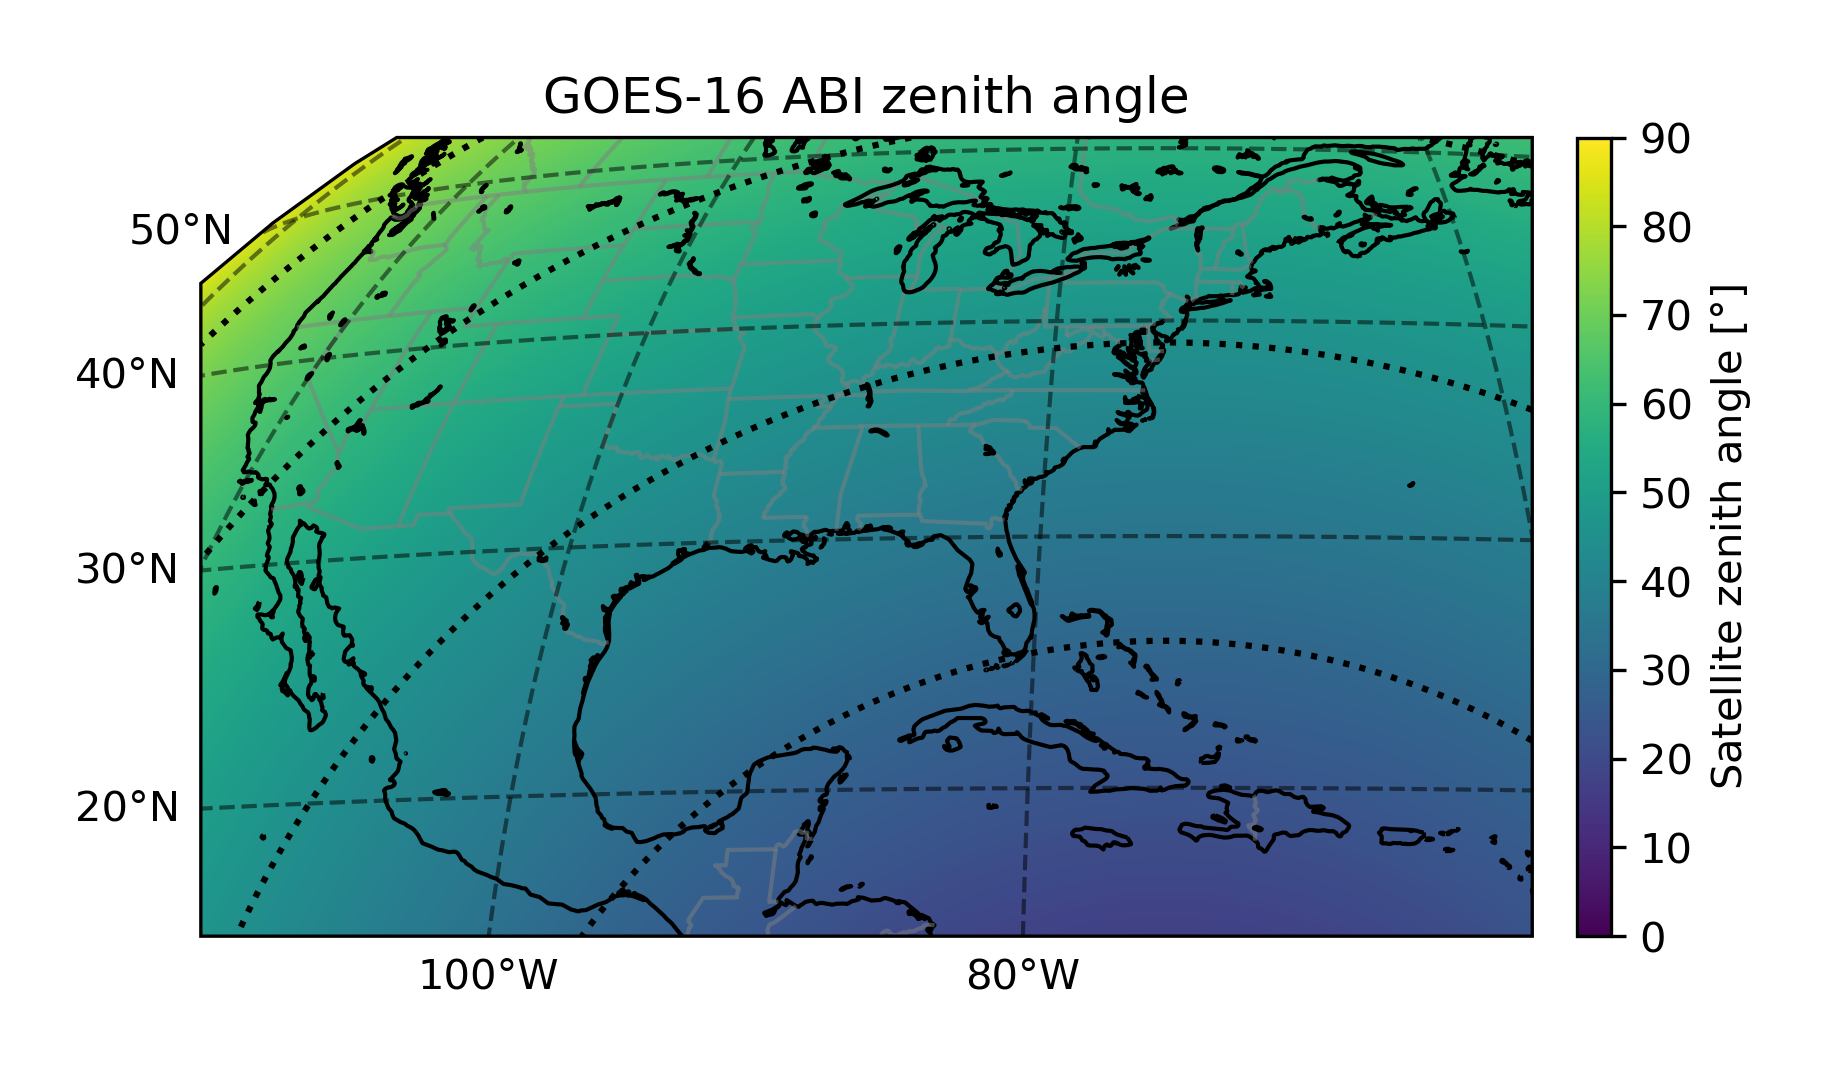
\includegraphics[width=\textwidth]{figures/chapter2_01.png}
    \caption[
    The sensor zenith angle of \acrshort{goes}-16 \acrshort{abi} observations across the \acrshort{conus} domain
    ]{
    The sensor zenith angle of \acrshort{goes}-16 \acrshort{abi} observations across the \acrshort{conus} domain. Dotted arcs are shown for each 15\,\textdegree interval of zenith angle.
    }
    \label{fig:abi_zenith_angles}
\end{figure}

To detect and track \acrshort{dcc}s across North America, \acrshort{abi} \acrshort{mcmip} data from the 6.2, 7.3, 10.4 and 12.4\,\unit{\mu m} channels observed in the \acrshort{conus} region is used, as described in section \ref{sec:abi_data}.
These observations span the full extent of the \acrshort{abi} \acrshort{conus} domain of 2,500~pixels E--W by 1,500~pixels N--S.
This domain covers a region of around 60--120\,\textdegree W in longitude and 15--50\,\textdegree N in latitude, covering an area of approximately 5,700 by 3,900\,\unit{km}.
Figure~\ref{fig:abi_zenith_angles} shows the satellite zenith angle of \acrshort{abi} observations across the \acrshort{conus} domain.
As the viewing angle increases the accurate detection and tracking of \acrshort{dcc}s becomes more difficult.
This is due to the confounding between vertical and horizontal motion, and also due to the area of each pixel increasing with the zenith angle.
The large sensor zenith angles in the North-West of the domain may introduce large errors in the detection and tracking algorithm, and so for the rest of this chapter only those \acrshort{dcc}s detected east of 110\,\textdegree W and south of 45\,\textdegree N are included in the analysis.

Five full years of data---from the start of 2018 to the end of 2022---are used to produce a dataset of detected \acrshort{dcc}s and their properties.
This period spans all complete years of operational data from \acrshort{goes}-16 \acrshort{abi}.
To improve to continuity of observations a gap-filling procedure is implemented.
If time gaps between observations of greater than 15 minutes are present, observations from the full-disc \acrshort{abi} scan are used to fill these gaps.
Full disc imagery is typically available every 10 or 15 minutes depending on the operating mode.
This gap filling is particularly important during the periods in which \acrshort{abi} uses its mode 4 scan pattern, in which no \acrshort{conus} domain scans are made, but the full-disc is scanned every 5 minutes.
Using the full-disc observations allows us to maintain temporal sampling throughout these periods.


\section{Method} \label{sec:conus_method}

Detection and tracking of convective cores and anvil cloud is performed using the \textit{tobac-flow} method \citep{jones_semi-lagrangian_2023} described in section~\ref{sec:tracking_method}.
Initial detection of \acrshort{dcc}s is performed separately over 24-hour periods spanning from 12:00:00~\acrshort{utc} (approximately 6am local time over North America) to the same time the next day.
This 24-hour period was dictated due to performance constraints, as the large domain combined with the high spatial and temporal resolution of \acrshort{abi} data results in a large memory requirement.
The start time corresponds with the minima of convective activity over land, and so was chosen in order to minimise the number of \acrshort{dcc}s missed at the start and end of the detection period.
Each period is extended by six \acrshort{abi} observations at each end to ensure at least one hour of overlap between successive days.

To track long-lived \acrshort{dcc}s that last beyond one day, a linking algorithm is used to combine \acrshort{dcc}s observed across multiple days.
The linking algorithm combines \acrshort{dcc}s detected at the same locations within the overlap period of two daily detection files.
Splitting and merging of objects is taken into account, so a single object which splits into two, or two objects which merge into one in the subsequent file are all considered a single, tracked object.
The linking algorithm is applied separately to each month of data for performance reasons.

%t
\begin{table}[b]
\centering
\begin{tabular}{ll}
\tophline
Core removed if:                                                    & Core invalid if: \\
\middlehline
Initial \acrshort{bt} -- final \acrshort{bt} \textless~8\,\unit{K}  & Intersects edge of domain \\
Lifetime \textless~15~minutes                                       & Intersects start of domain \\
Time gaps \textgreater~15~minutes                                   & Intersects end of domain \\
Maximum area \textgreater~10,000\,\unit{km\textsuperscript{2}}      & Adjacent to bad \acrshort{abi} data \\
Any NaN values in core properties                                   & \\
\bottomhline
\end{tabular}
\caption[
Validity criteria for detected cores
]{
Validity criteria for detected cores. Cores which flag any of the removal criteria are removed in their entirety from the dataset. Those which flag any of the invalid criteria are retained, but removed from subsequent analysis.}
\label{table:core_validity_criteria}
\end{table}

After linking, a processing step is applied to calculate the properties of detected cores and anvils at each step of their lifecycles.
Finally, core and anvil step properties are aggregated over each month of observation, and overall core and anvil properties are calculated.
During this final step quality flagging is performed to isolate detected features that fail one or more quality checks.
The quality criteria are split into two groups.
The first set of criteria---for core or anvil removal---removes features that cannot be verified as correctly tracked \acrshort{dcc}s due to bad data or a failure to meet the basic requirements for tracking described in chapter~\ref{chp:tracking_method}.
This may happen because there are large time gaps in the dataset, or missing data due to artifacts in the \acrshort{abi} observations.
Detected features which flag any of these criteria are removed from the aggregated dataset in their entirety.
This step in particular removes anvils which have no cores associated with them, or are not detected as initiating with a developing core.

The second set of criteria is used to identify detected cores or anvils which are not observed over their entire extent or lifecycle.
Cores and anvils which flag are of these criteria are still included within the aggregated properties dataset, but are removed from the analysis \acrshort{dcc} properties throughout this chapter.
Quality criteria for cores are listed in table \ref{table:core_validity_criteria}, and those for anvils in table \ref{table:anvil_validity_criteria}.


%t
\begin{table}[tb]
\centering
\begin{tabular}{ll}
\tophline
Anvil removed if:                               & Anvil invalid if: \\
\middlehline
No associated cores                             & Intersects edge of domain \\
Lifetime \textless~15~minutes                   & Intersects start of domain \\             
Time gaps \textgreater~15~minutes               & Intersects end of domain \\
Maximum area \textless~maximum core area        & Adjacent to bad \acrshort{abi} data \\
Anvil detected before initial core              & Associated with invalid cores \\
Anvil dissipated before final core ends         & Maximum area reached before end \\
Any NaN values in anvil properties              & ~~of initial core \\
\bottomhline
\end{tabular}
\caption[
Validity criteria for detected anvils
]{
Validity criteria for detected anvil. Anvils which flag any of the removal criteria are removed in their entirety from the dataset. Those which flag any of the invalid criteria are retained, but removed from subsequent analysis. The majority of anvils removed are due to have no associated cores, or because the anvil was observed before any developing cores.}
\label{table:anvil_validity_criteria}
\end{table}


The complete processing pathway is outlined by the following steps:

\begin{enumerate}
    \item Detection of cores and anvils in \acrshort{abi} observations over each 24-hour period.
    \item Linking of overlapping objects detected in subsequent 24-hour periods over each month.
    \item Calculation of core and anvil step properties. 
    \item Quality criteria applied to core and anvils, properties aggregated over each month
\end{enumerate}

Two datasets are produced. The first consists of daily core and anvil spatial maps, with step properties, produced by processing step 3. 
The second, consisting of aggregated monthly core and anvil properties, is produced by step 4.

\begin{figure}[tp]
    \centering
    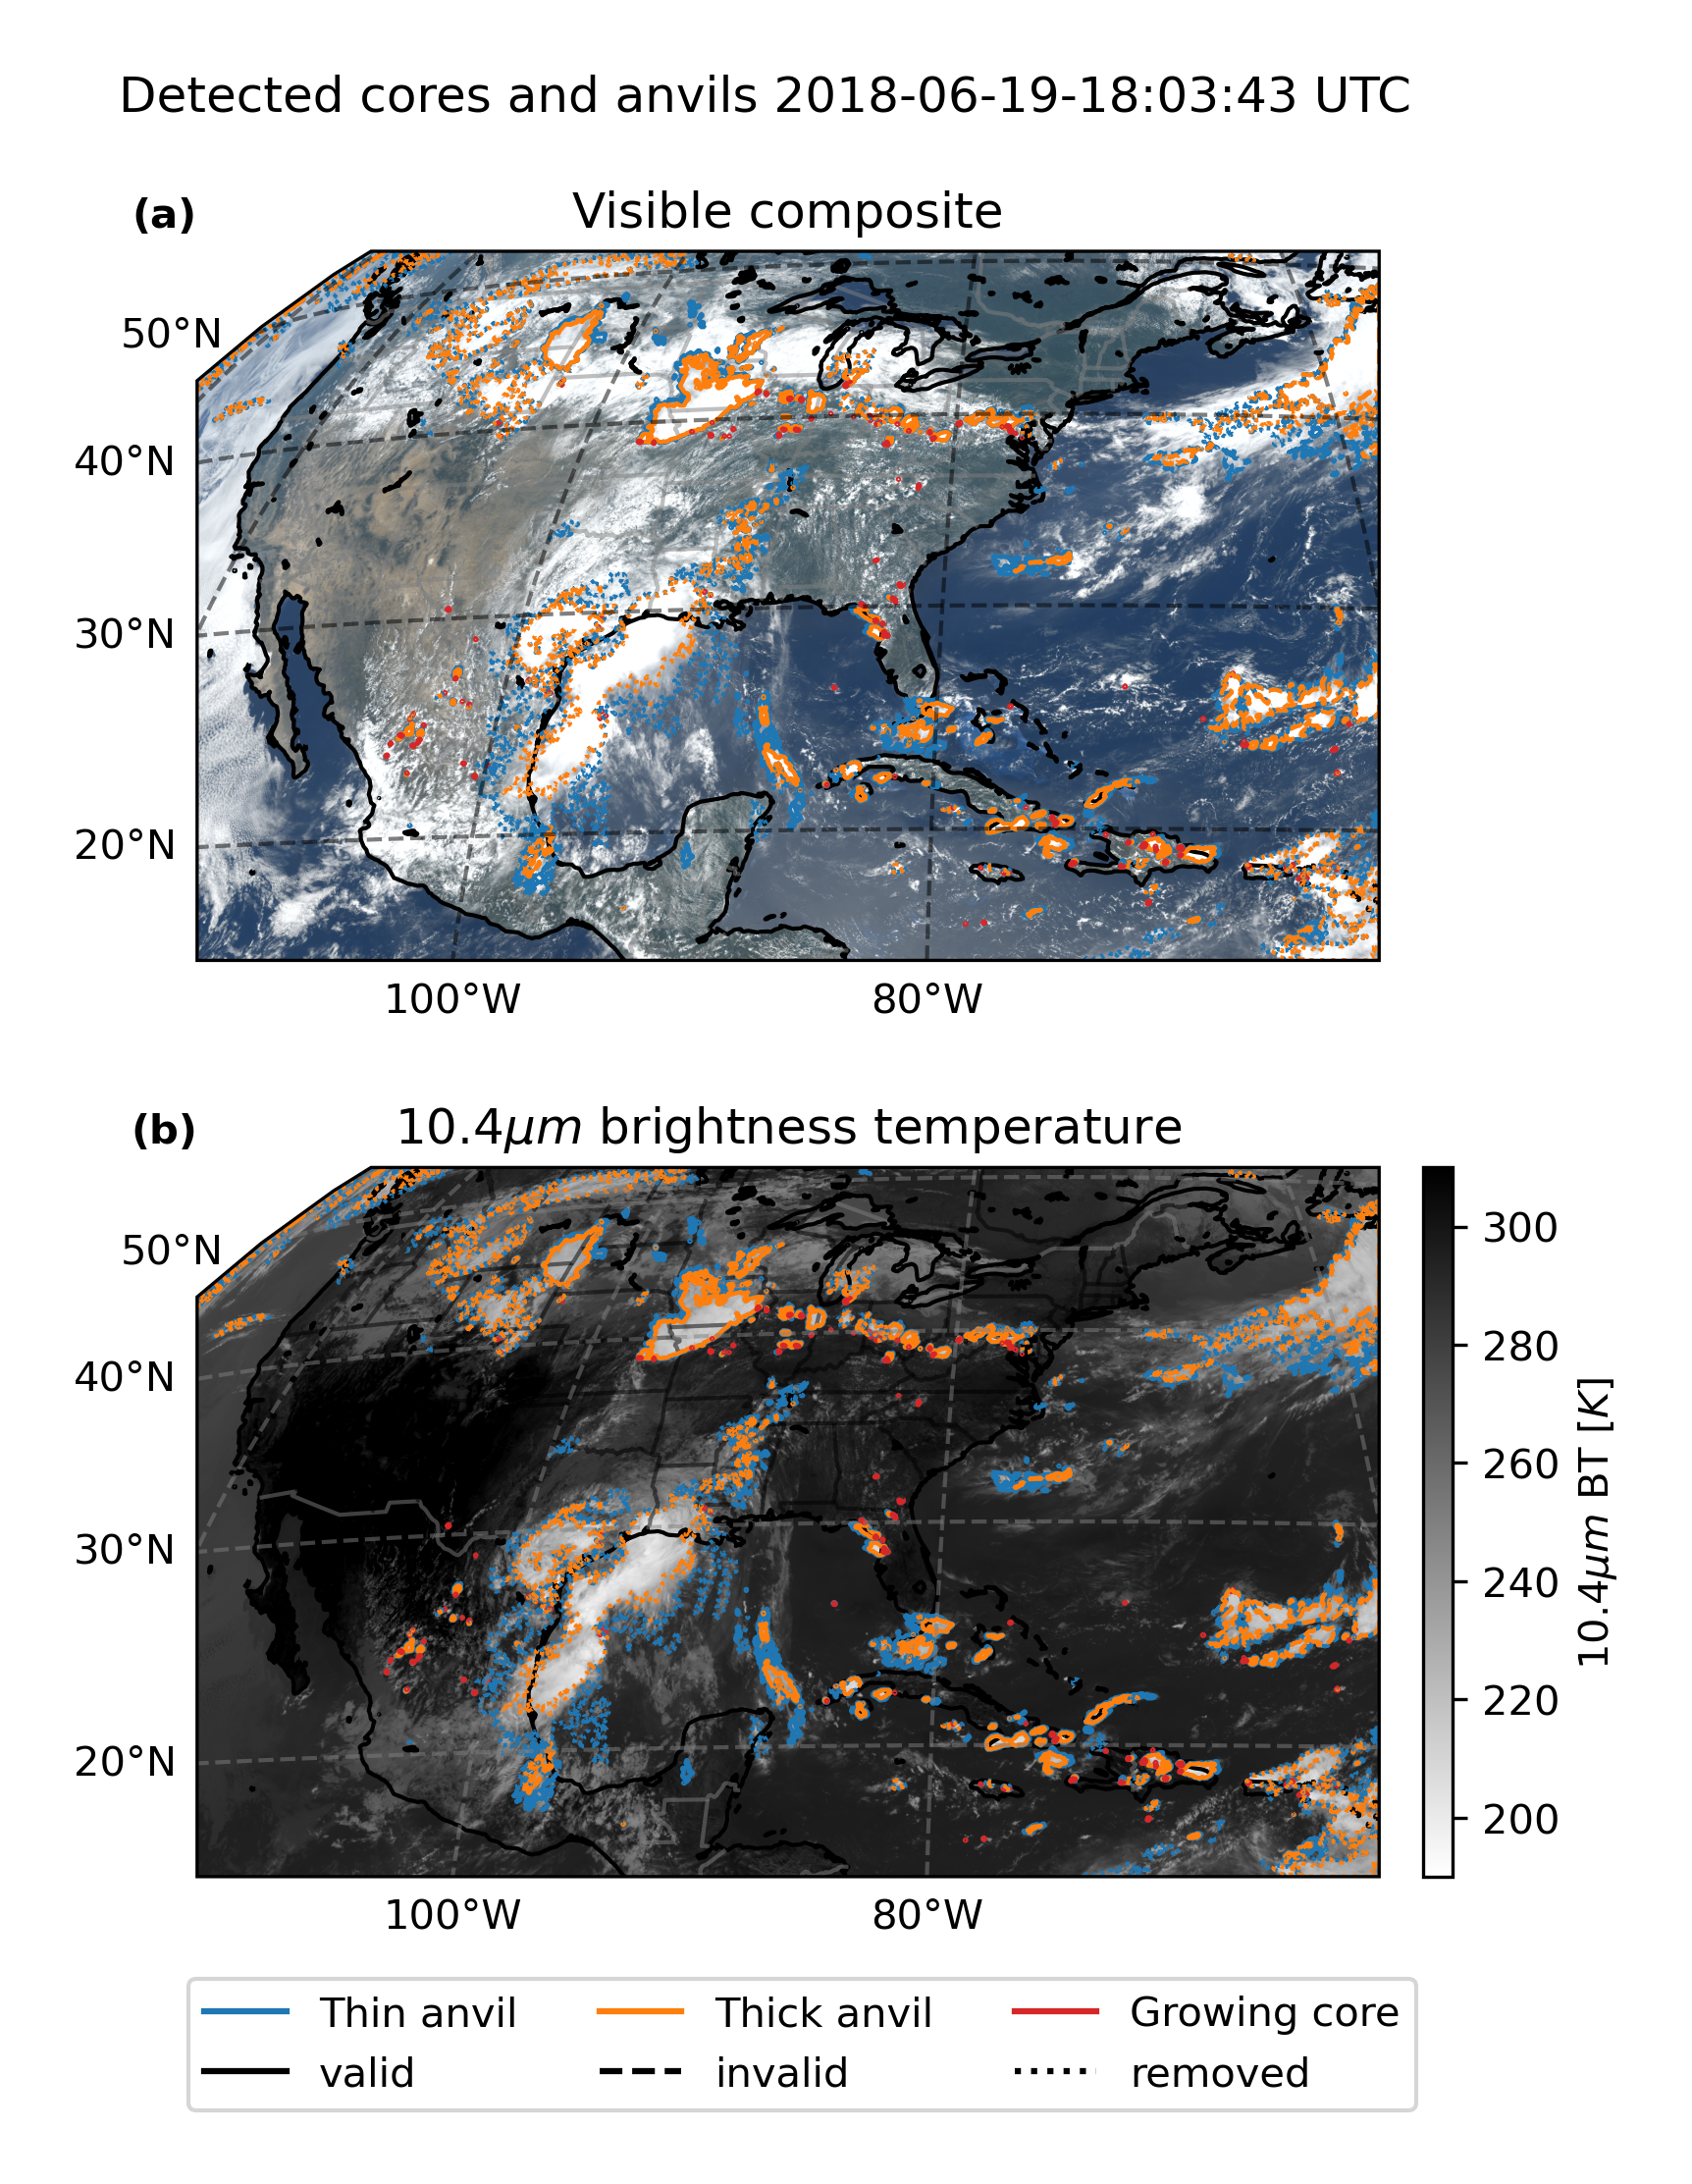
\includegraphics[width=\textwidth]{figures/chapter2_02.png}
    \caption[
    Detected cores and anvils from a snapshot of \acrshort{goes}-16 \acrshort{conus} domain observations
    ]{
    Detected cores and anvils from a snapshot of \acrshort{goes}-16 \acrshort{conus} domain observations. Cores and anvils removed from the aggregated dataset are shown with dotted outlines. Those which are flagged as invalid are shown with dashed outlines. Detected features are shown against (a) visible composite imagery and (b) 10.4\,\unit{\mu m} \acrshort{bt}
    }
    \label{fig:conus_detected_dccs}
\end{figure}

Figure~\ref{fig:conus_detected_dccs} shows an example of detected cores and anvils over the \acrshort{conus} region, against backgrounds of composite visible imagery (fig.~\ref{fig:conus_detected_dccs}\,a) and 10.4\,\unit{\mu m} \acrshort{bt} (fig.~\ref{fig:conus_detected_dccs}\,b).
Cores and anvils which are removed from the aggregated dataset are outlined with dotted lines, and those which are marker invalid are shown with dashed outlines.
The large, organised convective system centred at 95\,\textdegree W, 27\,\textdegree N has been removed as it is intersected by a scan-line artifact later in its lifetime.
The \acrshort{dcc}s observed along the eastern edge of the domain have been marked invalid as, while they are considered true detections of \acrshort{dcc}s, they intersect the edge of the domain.

Over the five-year observing period a total of 3,877,130 cores are detected, of which 3,615,533 are consider valid, and 1,643,030 are linked with an anvil cloud. 
A total of 648,345 anvils are detected, of which 391,050 are valid, and these valid anvils contain 792,522 cores.
The disparity in the number of valid cores and the number of cores contained with valid anvils is due to additional filtering applied to the anvils.
As the larger and longer-lived anvils are more likely to intersect the edges of the domain, they are more likely to be marked invalid than the cores.
In these cases, the cores themselves are valid for analysis, as their evolution is observed in its entirety, but exclude the anvil itself from analysis as we do not capture its entire extent and lifetime.
The exclusion of anvils that intersect the edges of the domain introduces a bias towards removing larger, long-lived systems near the edge of the domain, which should be considered when assessing the properties of the observed \acrshort{dcc}s.


\section{Results}


\subsection{Distributions and properties of developing convective cores} \label{sec:core_properties}

%f
\begin{figure}[tp]
    \centering
    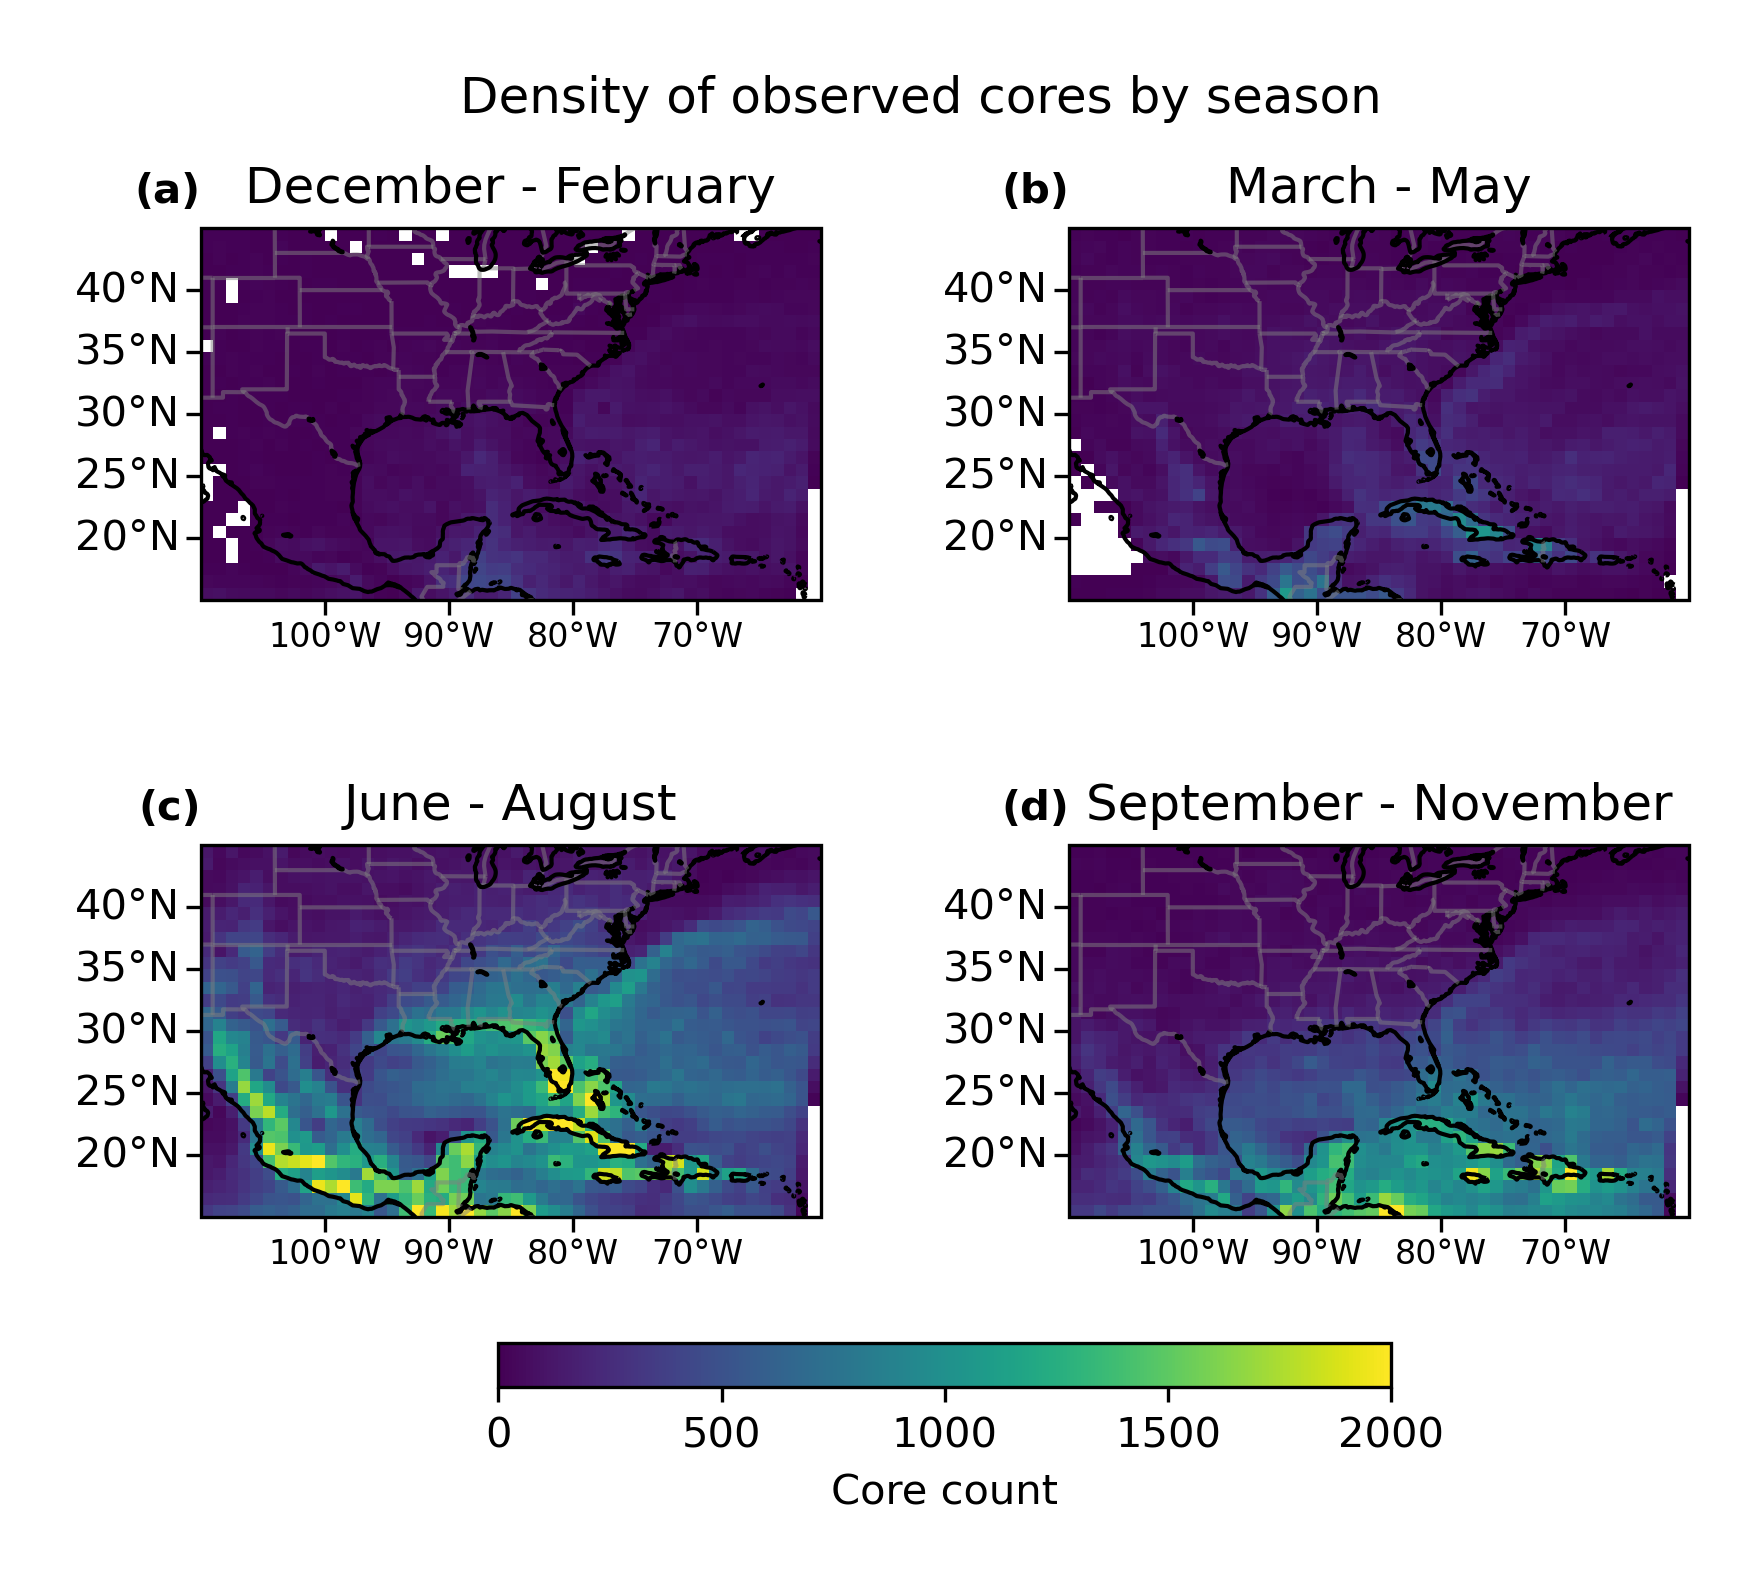
\includegraphics[width=\textwidth]{figures/chapter2_03.png}
    \caption[
    The spatial distribution of observed cores by season
    ]{
    The spatial distribution of observed cores, broken down by season and accumulated into 1\texttimes1\textdegree\ grid boxes of latitude and longitude. The density of observed cores is greatest during summer (c) and smallest during winter (a).
    }
    \label{fig:core_density_by_season}
\end{figure}

To begin, the distribution of detected \acrshort{dcc} cores throughout the dataset is investigated.
Figure~\ref{fig:core_density_by_season} shows the distribution of observed cores over North America separated by season.
Large variations in the spatial distribution of cores can be observed across the different seasons.
Overall, in winter and spring (fig.~\ref{fig:core_density_by_season}\,a,b) there are lower rates of observed \acrshort{dcc}s than in the summer and autumn (fig.~\ref{fig:core_density_by_season}\,c,d).

In winter (fig.~\ref{fig:core_density_by_season}\,a) the majority of convection observed occurs over the ocean, particularly in the areas of the Gulf of Mexico and West Atlantic associated with warm currents.
In spring (fig.~\ref{fig:core_density_by_season}\,b), a similar pattern shows over the ocean, and there is also an increase in convection detected over land in the Caribbean, Mexico and the central and southern \acrshort{usa}.
In summer (fig.~\ref{fig:core_density_by_season}\,c) there is a large increase in convection over land and ocean, with the highest rates of convection of any season.
There are, in particular, high rates of convection over Mexico, the Caribbean, the southern \acrshort{usa} (Florida in particular) and adjacent ocean regions.
In Autumn (fig.~\ref{fig:core_density_by_season}\,d) there is a large reduction in the number of convective cores detected over land regions.
The number of detections over the ocean remains high, however, indicating a possible lag in the seasonal cycle of convection over oceans compared to that over land.

%f
\begin{figure}[tp]
    \centering
    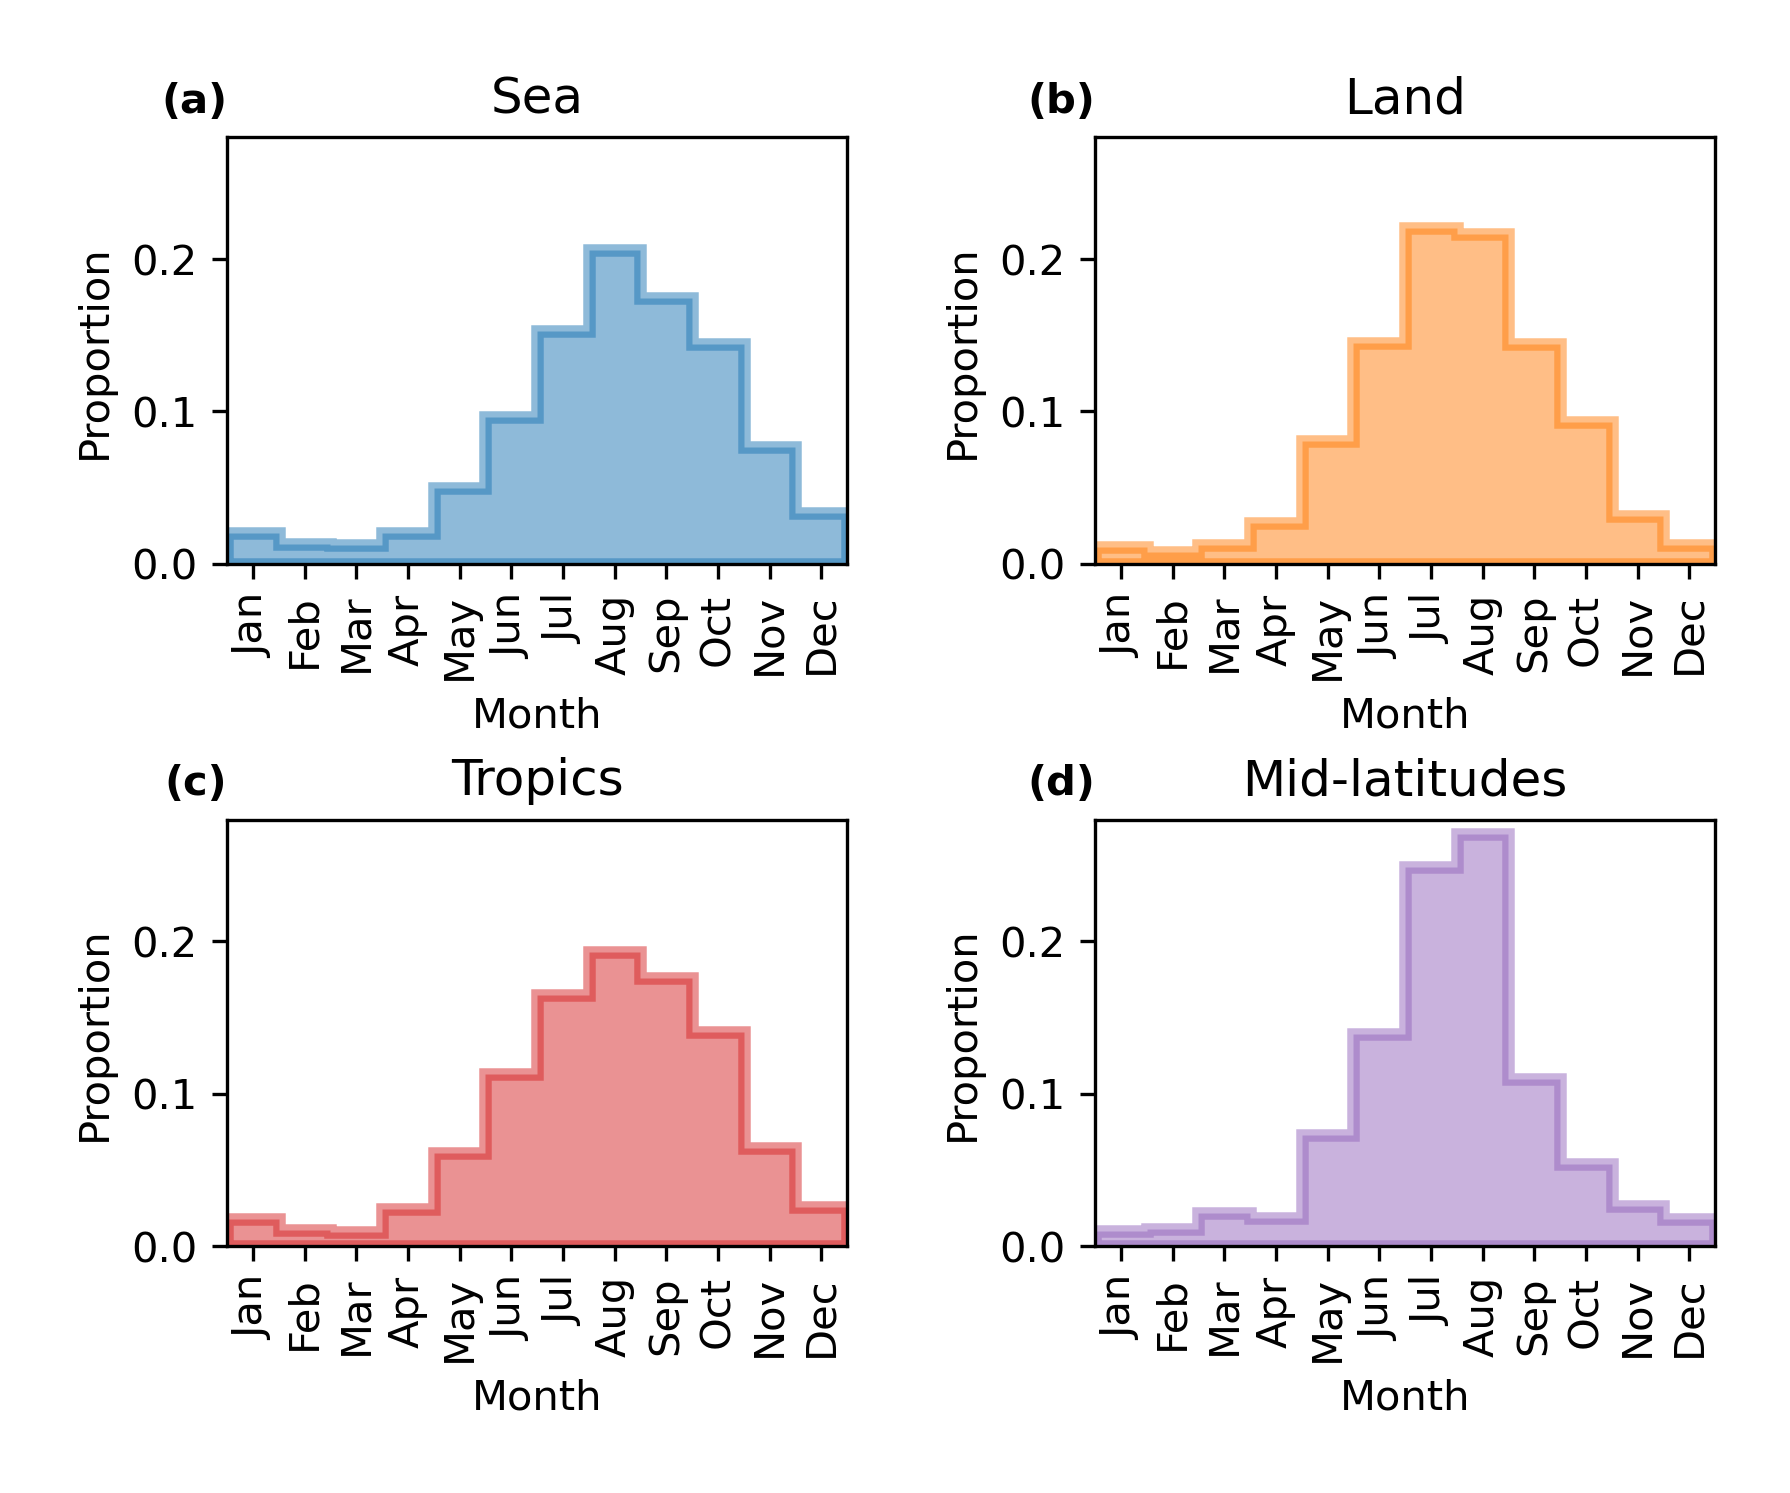
\includegraphics[width=\textwidth]{figures/chapter2_04.png}
    \caption[
    Monthly distributions of the proportion of cores detected each month over land, sea, tropics and mid-latitudes
    ]{
    Monthly distributions of the proportion of cores detected each month over (a) sea, (b) land, (c) tropics (\textless 30\,\textdegree N) and (d) mid-latitudes (\textgreater 30\,\textdegree N).
    }
    \label{fig:core_annual_land_sea}
\end{figure}


Figure~\ref{fig:core_annual_land_sea} shows the proportion of cores detected in each month over the annual cycle for land and sea regions.
Both land and sea regions show a peak of convective activity in the summer, and a low in the winter months.
However, as suggested by fig.~\ref{fig:core_density_by_season}, there is a time lag of about 1 month between the annual cycle of convection over land and that over the ocean, likely due to the time lag in ocean heating.
Comparing the tropics and mid-latitudes, the monthly distribution of convection is much more sharply focused on July--August in the mid-latitudes compared to the broader distribution seen in the tropics.


%f
\begin{figure}[tp]
    \centering
    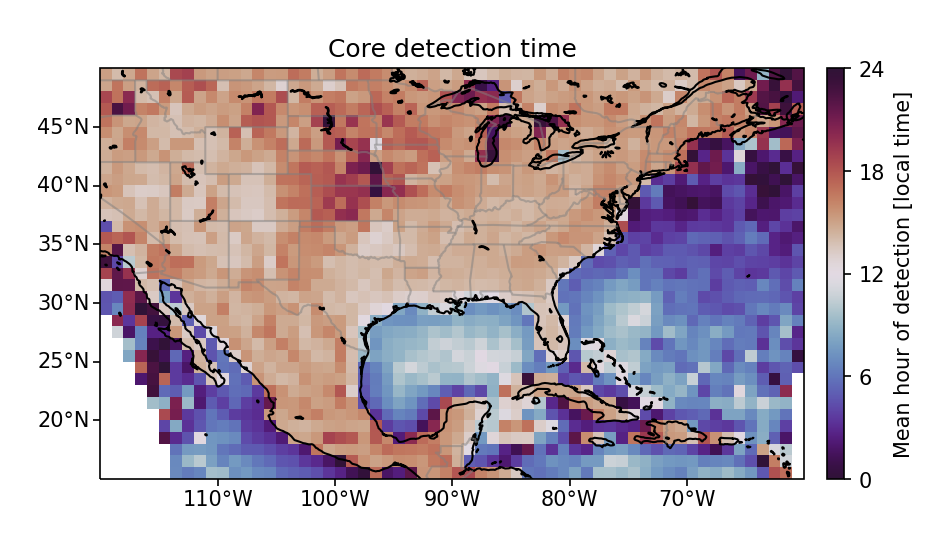
\includegraphics[width=\textwidth]{figures/chapter2_05.png}
    \caption[
    The average speed and direction of propagation of cores
    ]{
    The average speed and direction of propagation of cores observed within each 1\texttimes1\textdegree\ grid box. The colouring shows the average speed of propagation, and the red arrows show the average direction for each 2\texttimes2\textdegree\ grid box}
    \label{fig:core_propagation_map}
\end{figure}

Figure~\ref{fig:core_propagation_map} shows the average speed of propagation for cores observed in each 1-degree grid box, with the average direction of propagation shown by arrows for each 2-degree grid box.
There is a clear change in the direction of propagation from an easterly motion in the tropics (below 25\,\textdegree N) to a south-westerly motion in the mid-latitudes.

%f
\begin{figure}[tp]
    \centering
    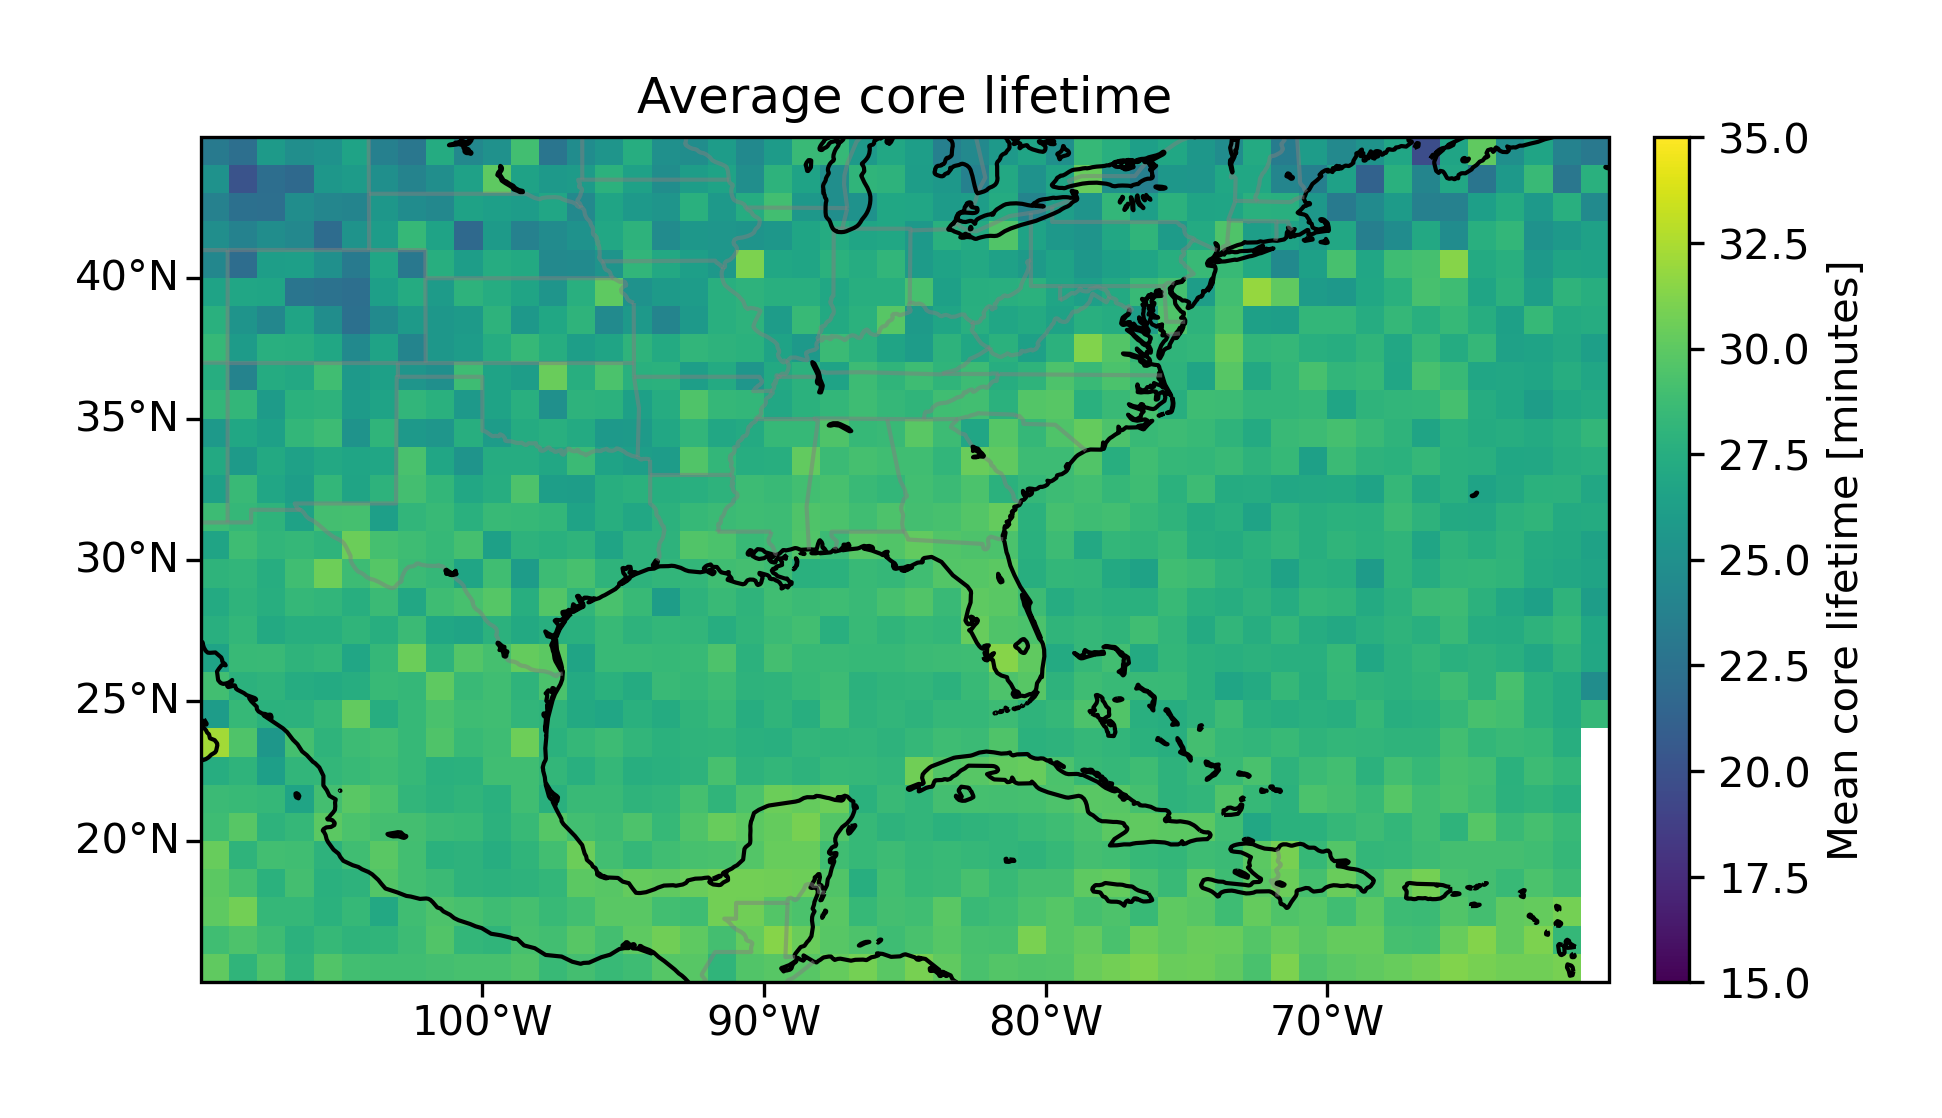
\includegraphics[width=\textwidth]{figures/chapter2_06.png}
    \caption[
    A map showing the mean lifetime in minutes of cores within each 1\texttimes1
    \textdegree\ grid box
    ]{
    A map showing the mean lifetime in minutes of cores within each 1\texttimes1
    \textdegree\ grid box.
    }
    \label{fig:core_lifetime_map}
\end{figure}

Figure \ref{fig:core_lifetime_map} displays the mean lifetime of observed cores over each 1-degree box of latitude and longitude.
The lifetime is defined as the period of time over which each core is detected, which represents the time in which to core is developing vertically.
Convection will continue in the core after this point, but the motion of the cloud top will instead be a horizontal divergence of the anvil.
The average lifetimes appear mostly uniform across the domain, with a small reduction with increasing latitude.
This reduction in the lifetime of the developing core at higher latitudes is likely due to the lower tropopause height restricting the vertical development of the cores.
Similarly, there is a slight reduction in average lifetime over the more mountainous, inland regions of Mexico compared to the adjacent coastal regions.
This again may be linked to the reduction in the depth of the convective cores, although in this case due to an increased surface height rather than a lower tropopause.


%f
\begin{figure}[tp]
    \centering
    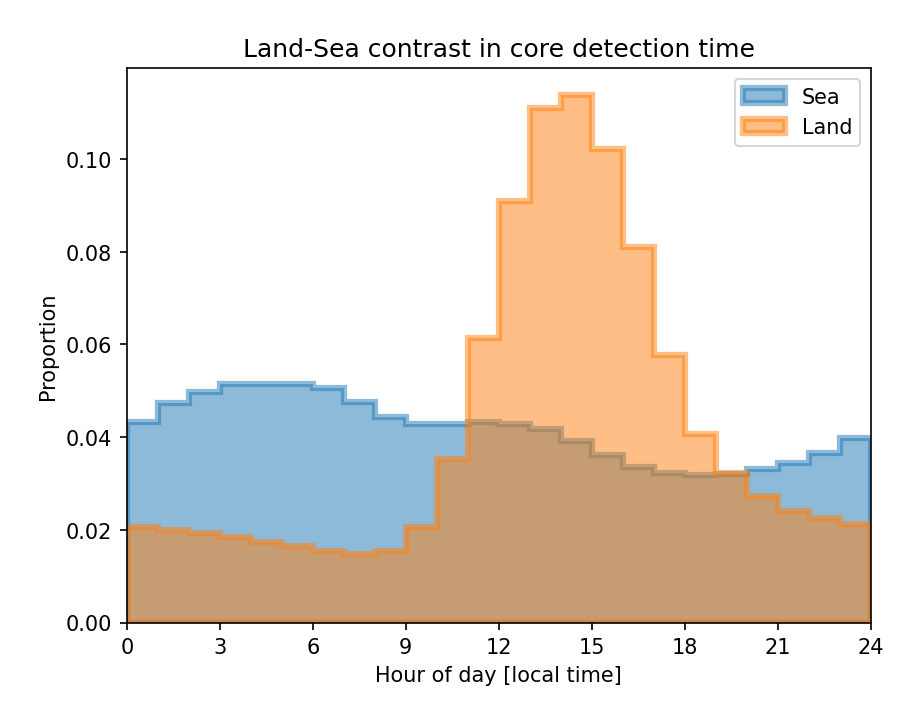
\includegraphics[width=\textwidth]{figures/chapter2_07.png}
    \caption[
    A map of the average maximum core cooling rate for each 1\texttimes1
    \textdegree\ grid box
    ]{
    A map of the  average maximum core cooling rate for each 1\texttimes1
    \textdegree\ grid box.
    }
    \label{fig:core_cooling_rate_map}
\end{figure}

Figure~\ref{fig:core_cooling_rate_map} shows the average cooling rate of observed cores.
The contrasts here are more pronounced that those shown in fig.~\ref{fig:core_lifetime_map}.
There is a reduction in the average cooling rate with latitude, likely due to the reduction in solar heating and hence lower \acrshort{cape}.
Orography also has a factor, with lower cooling rates observed over the mountains of Mexico and the North American Rockies.
The largest average core cooling rates are observed in in coastal regions, indicating potential land--sea interactions.

%f
\begin{figure}[tp]
    \centering
    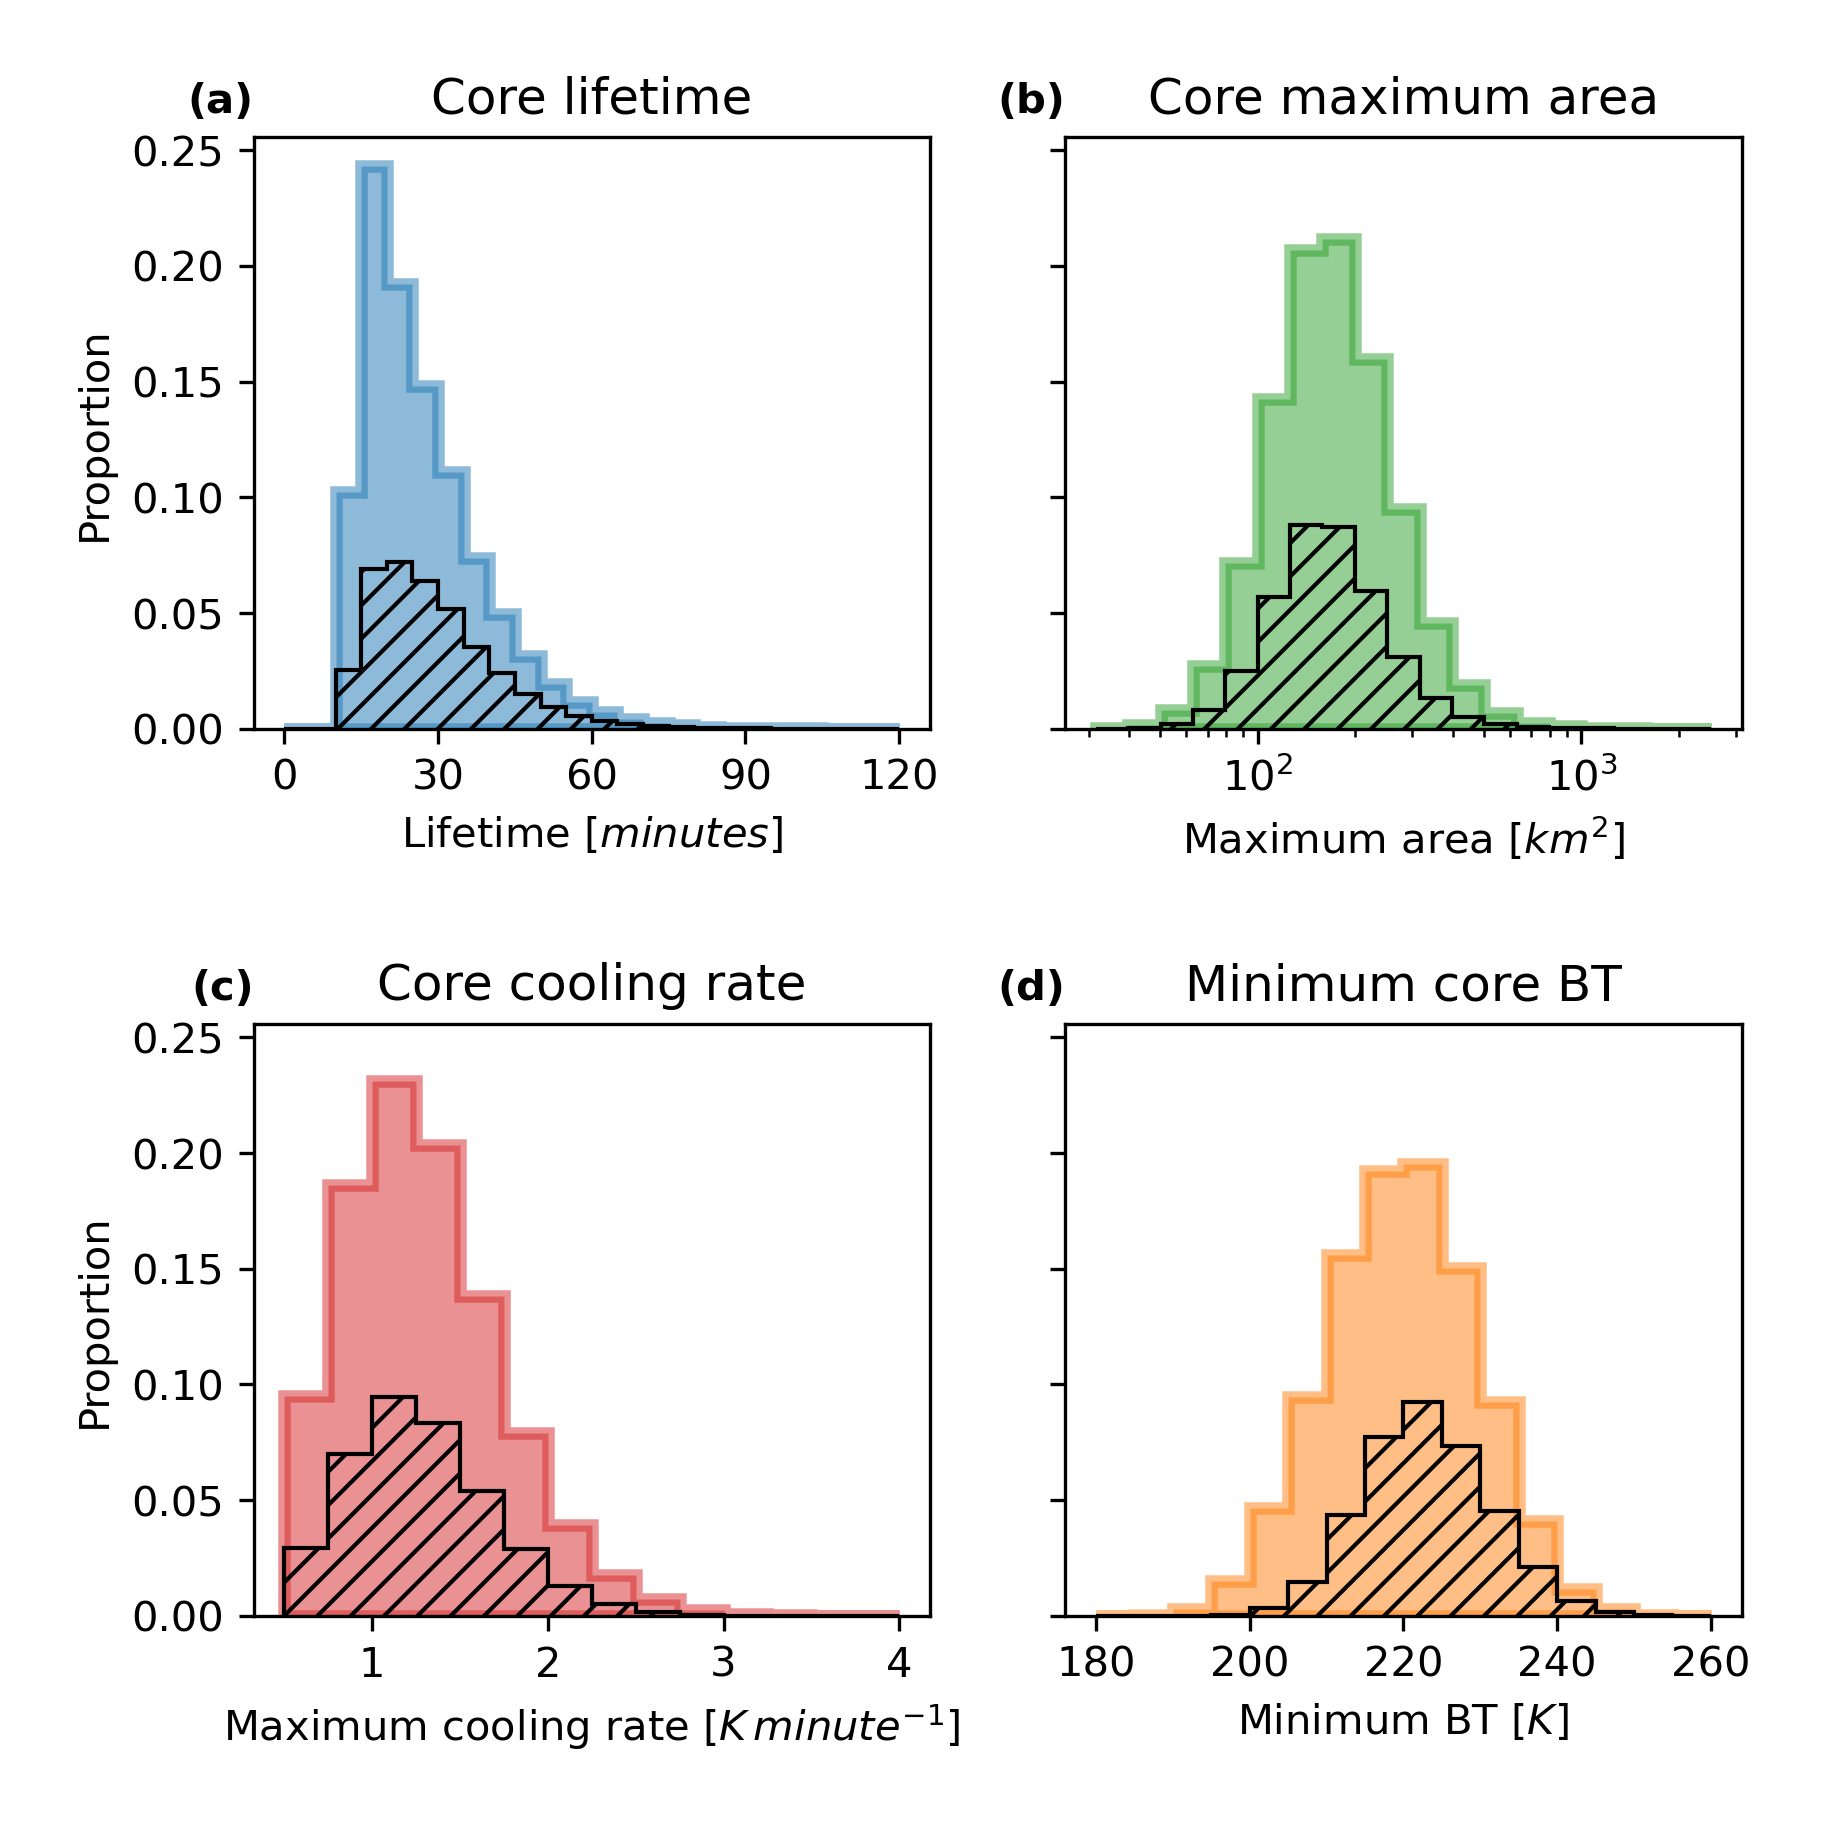
\includegraphics[width=\textwidth]{figures/chapter2_08.png}
    \caption[
    Histograms showing the distributions of observed core lifetimes, maximum areas, cooling rates and \acrshort{bt}
    ]{
    Histograms showing the distributions of observed (a) core lifetime, (b) maximum area, (c) maximum cooling rate, (d) and minimum \acrshort{bt}. The hatched areas show the proportion of each distribution consisting of the initial detected cores within each tracked \acrshort{dcc}.
    }
    \label{fig:core_properties}
\end{figure}

Figure~\ref{fig:core_properties} shows the distributions of lifetime (fig.~\ref{fig:core_properties}\,a), maximum area (fig.~\ref{fig:core_properties}\,b), cooling rate (fig.~\ref{fig:core_properties}\,c), and minimum \acrshort{bt} (fig.~\ref{fig:core_properties}\,d).
There is a peak in the observed lifetime of cores between 15 and 20 minutes, with a large tail extending beyond 60 minutes in some cases.
Note that due to the requirement of a minimum of three consecutive observations, cores lasting less than 10 minutes will not be detected, truncating the distribution.
In fig.~\ref{fig:core_properties}\,b the maximum core area peaks around 150--200\,\unit{km\textsuperscript{2}}, representing cores approximately 12--14 km in diameter.
Figure~\ref{fig:core_properties}\,c shows that the core cooling rate peaks at values of 1--1.25\,\unit{K minute\textsuperscript{-1}}, representing vertical cloud top velocities of approximately 2.5--3\,\unit{ms\textsuperscript{-1}}.
The distribution is slightly truncated by the requirement for detected cores to have a cooling rate of at least 0.5\,\unit{K minute\textsuperscript{-1}}.
Finally, the minimum core \acrshort{bt} (fig.~\ref{fig:core_properties}\,d) peaks around 220\,\unit{K}, the temperature of the radiative tropopause \citep{jeevanjee_simple_2020}

The hatched areas in fig.~\ref{fig:core_properties} show the proportion of each distribution consisting of the initial cores of tracked \acrshort{dcc}s.
For these initial cores there is no possibility of the observations being masked by an overlaying anvil cloud, these are expected to provide the most complete measurements of developing core properties.
For the lifetime, maximum area and cooling rate these show close similarities to the shape of the distribution for all cores, indicating that masking due to anvils does not significantly affect the ability to observe the core properties.
For the minimum core \acrshort{bt}, the initial cores tend to have warmer \acrshort{bt} than later cores, indicating an increased presence of cold cores and overshooting tops in organised convection.

%f
\begin{figure}[tp]
    \centering
    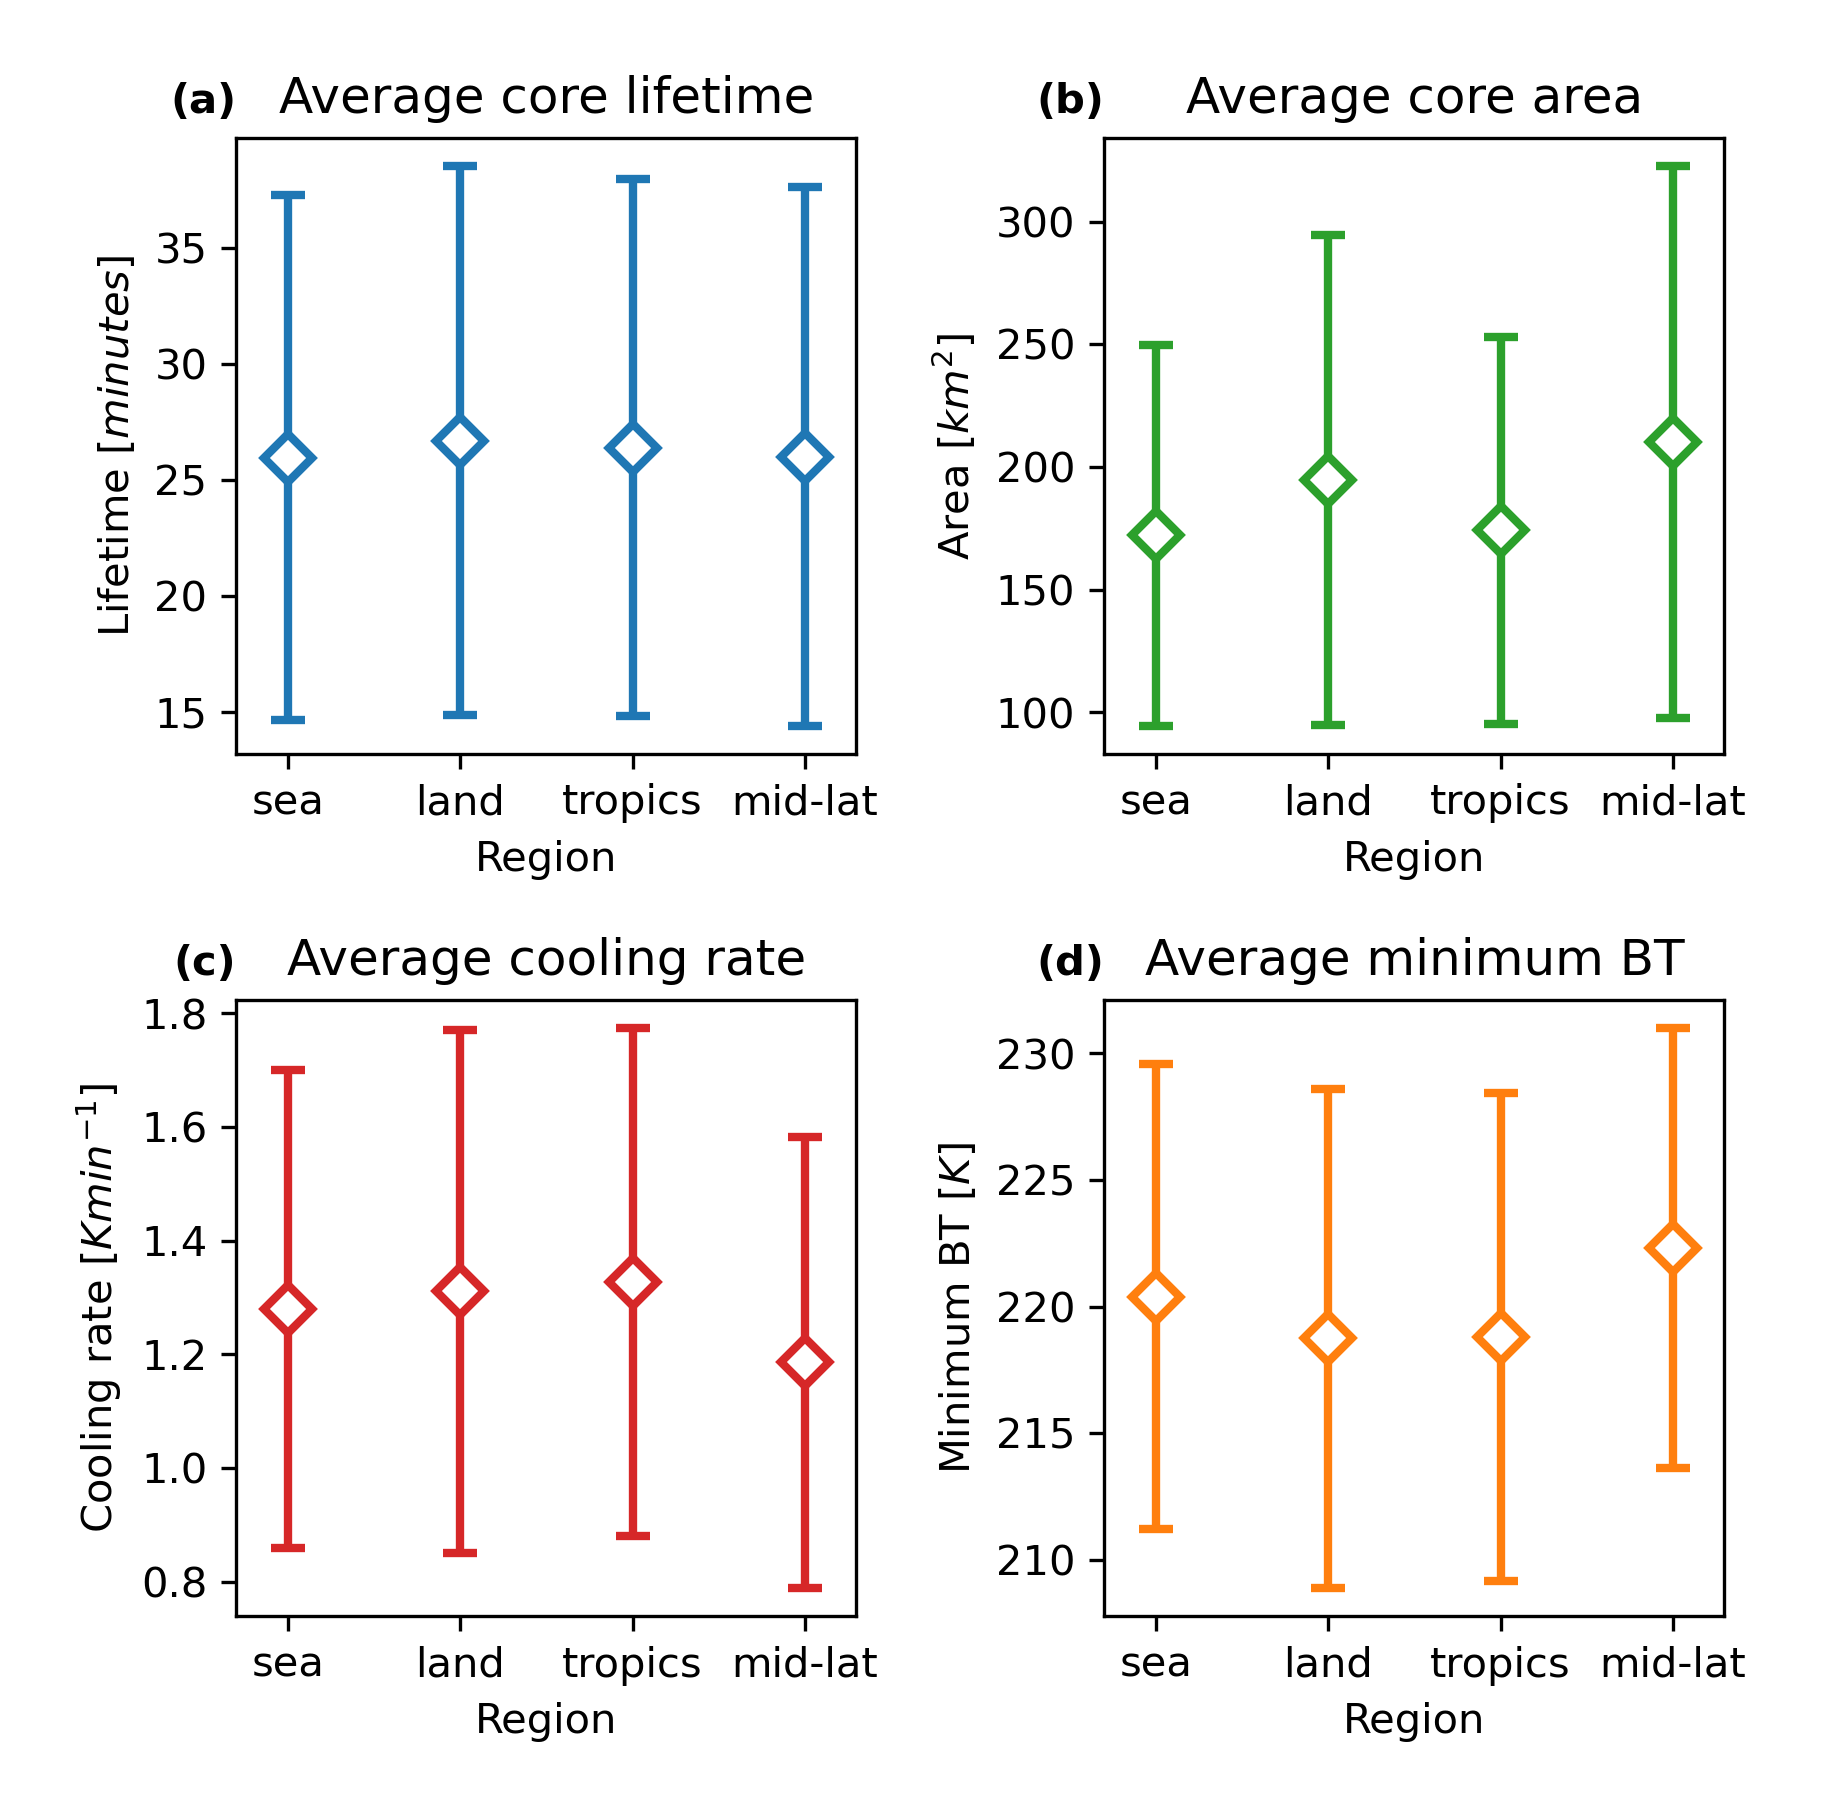
\includegraphics[width=0.75\textwidth]{figures/chapter2_09.png}
    \caption[
    The mean observed lifetimes, maximum areas, cooling rates and \acrshort{bt} for cores detected over land, sea, tropics and mid-latitudes
    ]{
    The mean observed (a) lifetime, (b) maximum area, (c) maximum cooling rate, (d) and minimum \acrshort{bt} for cores detected over land, sea, tropics and mid-latitudes. Error bars show to standard deviation of each point.
    }
    \label{fig:core_region_mean_properties}
\end{figure}

Figure~\ref{fig:core_region_mean_properties} shows how the mean core lifetime, maximum area, cooling rate and \acrshort{bt} vary between different regions.
There is little difference in the mean core lifetime between regions, echoing the results seen in fig.~\ref{fig:core_lifetime_map}.
Maximum core area is larger over land than sea, and larger in the mid-latitudes than in the tropics.
There is little difference in the cooling rate between sea and land, but on average cores in the tropics cool $\sim$0.2\,\unit{K minute\textsuperscript{-1}} faster than those in the mid-latitudes.
There is a small difference in the minimum \acrshort{bt} of cores observed over land and ocean, with the former $\sim$1.5\,\unit{K} colder than the latter.
A more noticeable difference is seen with latitude, with cores in the tropics having, on average, minimum \acrshort{bt} $\sim$5\,\unit{K} colder than those in the mid-latitudes.

Overall, fig.~\ref{fig:core_region_mean_properties} show differences in core intensity between land and ocean, and between the tropics and mid-laitudes, with these differences most prominent in the minimum \acrshort{bt}.
However, these differences may result from changes in different properties of the cores as the difference in cooling rate between tropics and mid-latitudes is not seen when comparing sea and land.

%f
\begin{figure}[tp]
    \centering
    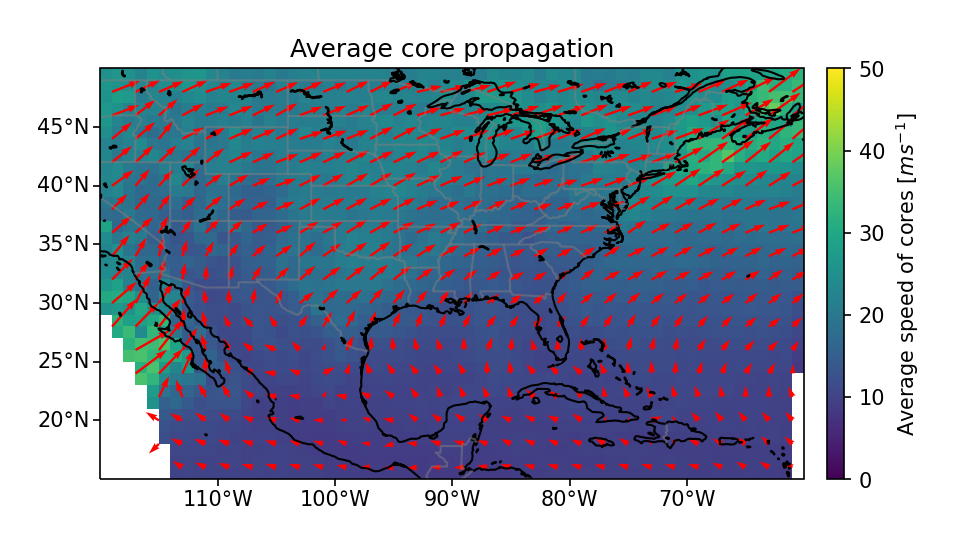
\includegraphics[width=0.75\textwidth]{figures/chapter2_10.png}
    \caption[
    Average core lifetime and minimum \acrshort{bt} with increasing core cooling rate
    ]{
    Average core lifetime (a) and minimum \acrshort{bt} (b) with increasing core cooling rate. Error bars show the variance of the data, while the shaded area shows the standard error of the mean.
    }
    \label{fig:core_cooling_rate_relations}
\end{figure}


Figure~\ref{fig:core_cooling_rate_relations}\,a compares how the average lifetime of detected cores changes with their maximum observed cooling rate.
For low values of core cooling rate, there is a similar, positive linear relationship between cooling rate and lifetime between all regions, indicating that more intense convection leads to longer periods of cores being observed.
However, beyond cooling rates of around 1.5\,\unit{K minute\textsuperscript{-1}} there is a peak in the core intensity--height relationship, with larger cooling rates leading to shorter lifetimes.
This may be explained by the cores with faster cooling rates reaching their level of neutral buoyancy faster, and therefore showing cooling cloud tops for a shorter period of time.
The inflexion in the core lifetime may also explain why there are no apparent differences in average lifetime between different regions, despite differences in other convective properties.

Figure~\ref{fig:core_cooling_rate_relations}\,b shows how the minimum \acrshort{bt} changes with the maximum cooling rate of the core.
Unlike fig.~\ref{fig:core_cooling_rate_relations}\,a, there is a continuous decrease in \acrshort{bt} with core cooling rate, indicating that faster cooling rates tend to result in cores with colder \acrshort{ctt} and hence higher \acrshort{cth}.
Figure~\ref{fig:core_cooling_rate_relations}\,b also provides context for the results seen in fig.~\ref{fig:core_cooling_rate_relations}\,a.
If it is assumed that cores are detected around the freezing level (273\,\unit{K}), then the overall temperature change over the core lifetime ranges from $\sim$45\,\unit{K} for the least intense cores to $\sim$65\,\unit{K} for the most intense cores.
Although this continues to increase with the cooling rate, the proportional change is less than that of the core cooling rate itself.
As the core lifetime can be approximated as the core \acrshort{bt} change divided by the cooling rate, the larger proportional change in cooling rate will result in a shorter lifetime for more rapidly cooling cores.

% %f
% \begin{figure}[tp]
%     \centering
%     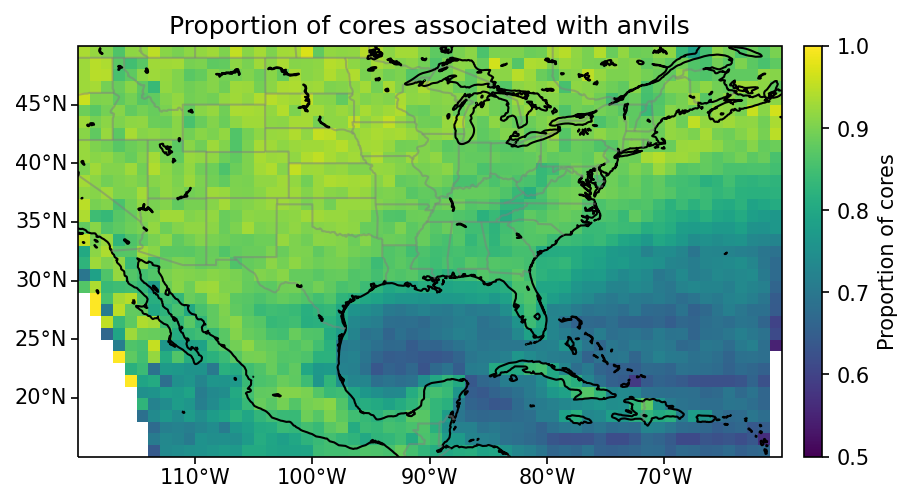
\includegraphics[width=\textwidth]{figures/ch2_04.png}
%     \caption[
%     The proportion of detection cores associated with anvils
%     ]{
%     The proportion of detection cores associated with anvils in each 1\texttimes1\textdegree\ grid box. In general, we see that the majority of cores over land are associated with anvils, while over the ocean a larger number are detected without anvils.
%     }
%     \label{fig:cores_with_anvils_map}
% \end{figure}

% Figure~\ref{fig:cores_with_anvils_map} shows the proportion of cores associated with anvil clouds.
% We see a clear land--sea contrast, with a much larger number of cores occurring without associated anvil clouds over the ocean than over land.

\subsection{Diurnal cycle of convective cores}

%f
\begin{figure}[tp]
    \centering
    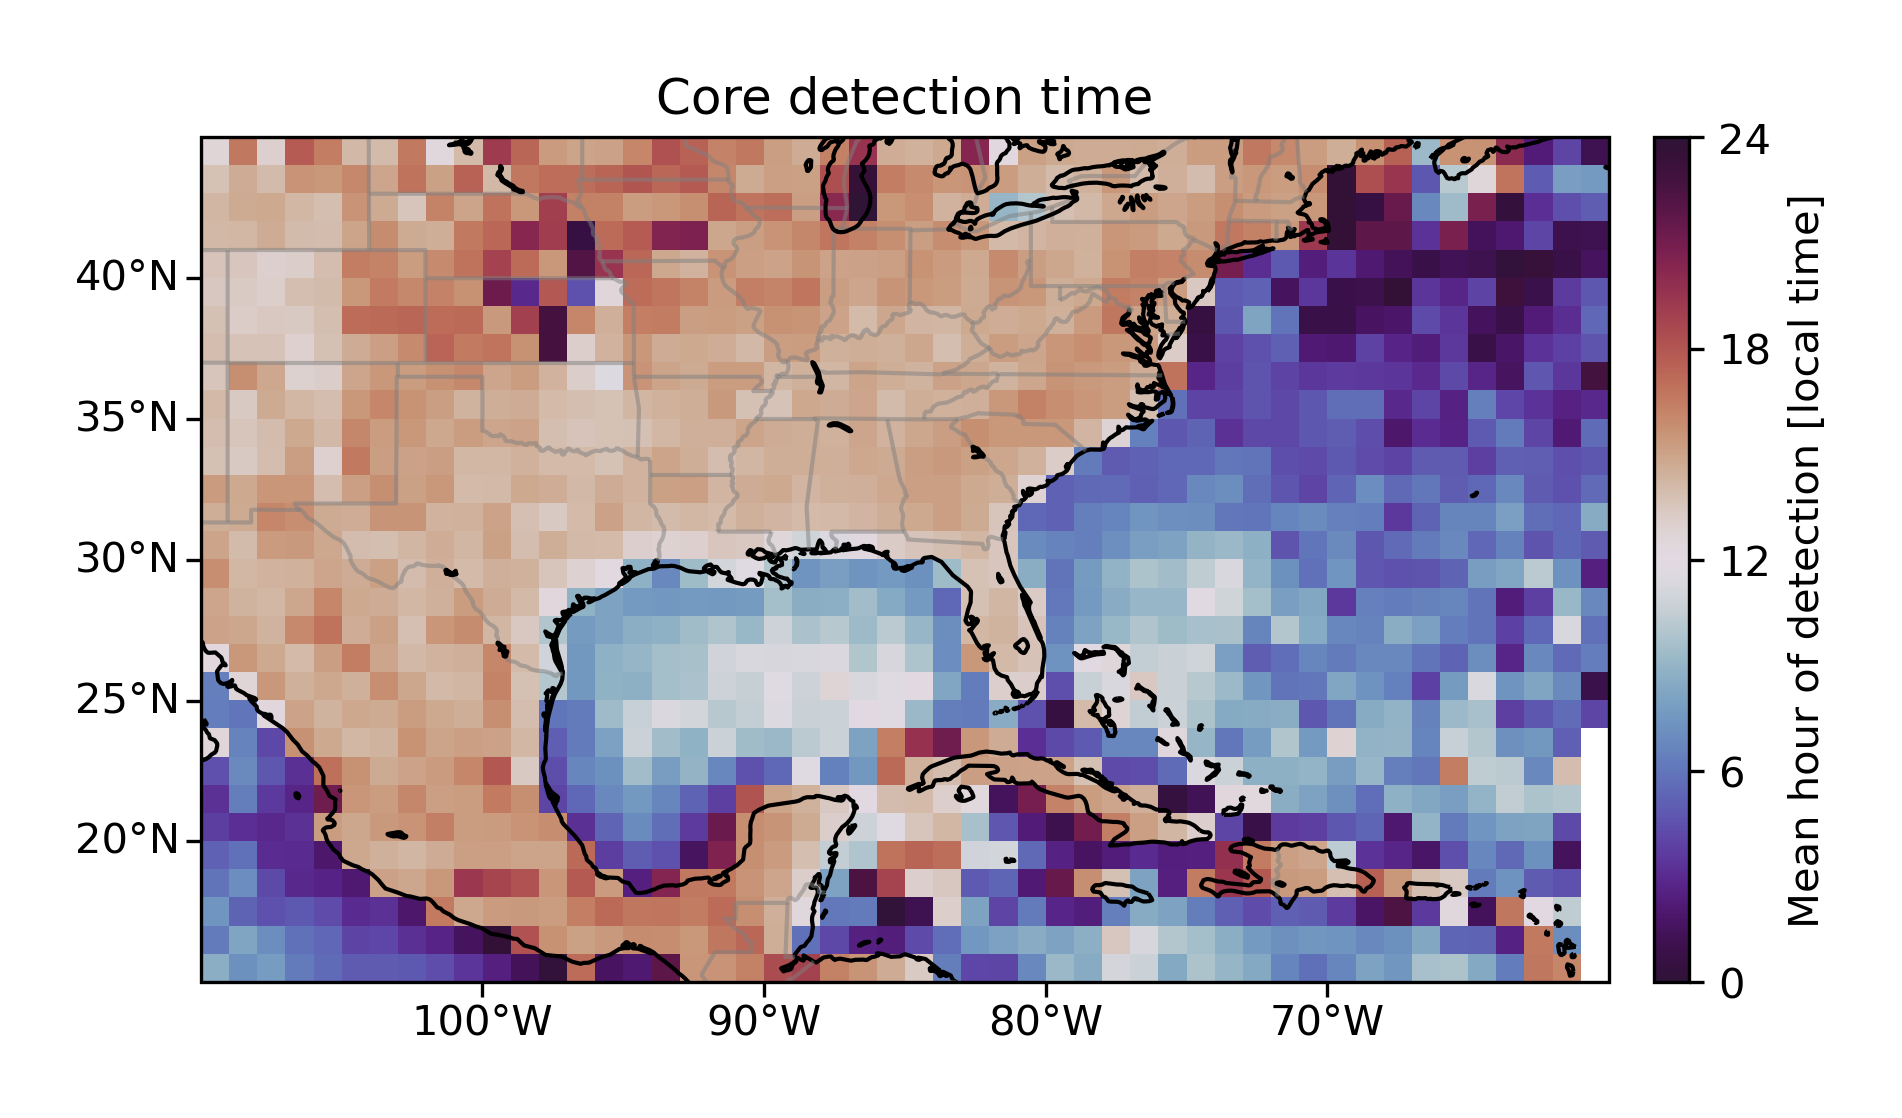
\includegraphics[width=\textwidth]{figures/chapter2_11.png}
    \caption[
    A map of average time of day of initiation of detected cores
    ]{
    The average time of day of initiation of cores observed within each 1\texttimes1\textdegree\ grid box. The time of initiation is calculated as the local solar time based on longitude, and the mean is calculated as the circular mean over a 24-hour period to account for the cyclical aspect of the hour of day.
    }
    \label{fig:core_detection_time_map}
\end{figure}

Figure~\ref{fig:core_detection_time_map}, shows the mean time of detection for cores detected within each 1-degree grid square.
The most notable feature in fig.~\ref{fig:core_detection_time_map} is the strong land-sea contrast, with the majority of land regions showing convective activity occurring during the afternoon, and the majority of ocean regions showing activity before midday.
In addition, there are a few major features of the detected time of initiation across both land and sea regions.
In coastal regions in the Gulf of Mexico and the Caribbean Sea, earlier initiation times are seen closer to coastlines, while regions further from land have average times of detection closer to midday.
Over the land there is also see a later time of initiation over the Northern Great Plains (90--100\,\textdegree W, 37--47\,\textdegree N).

% \subsubsection{Regional differences in the time of core detection}


%f
\begin{figure}[tp]
    \centering
    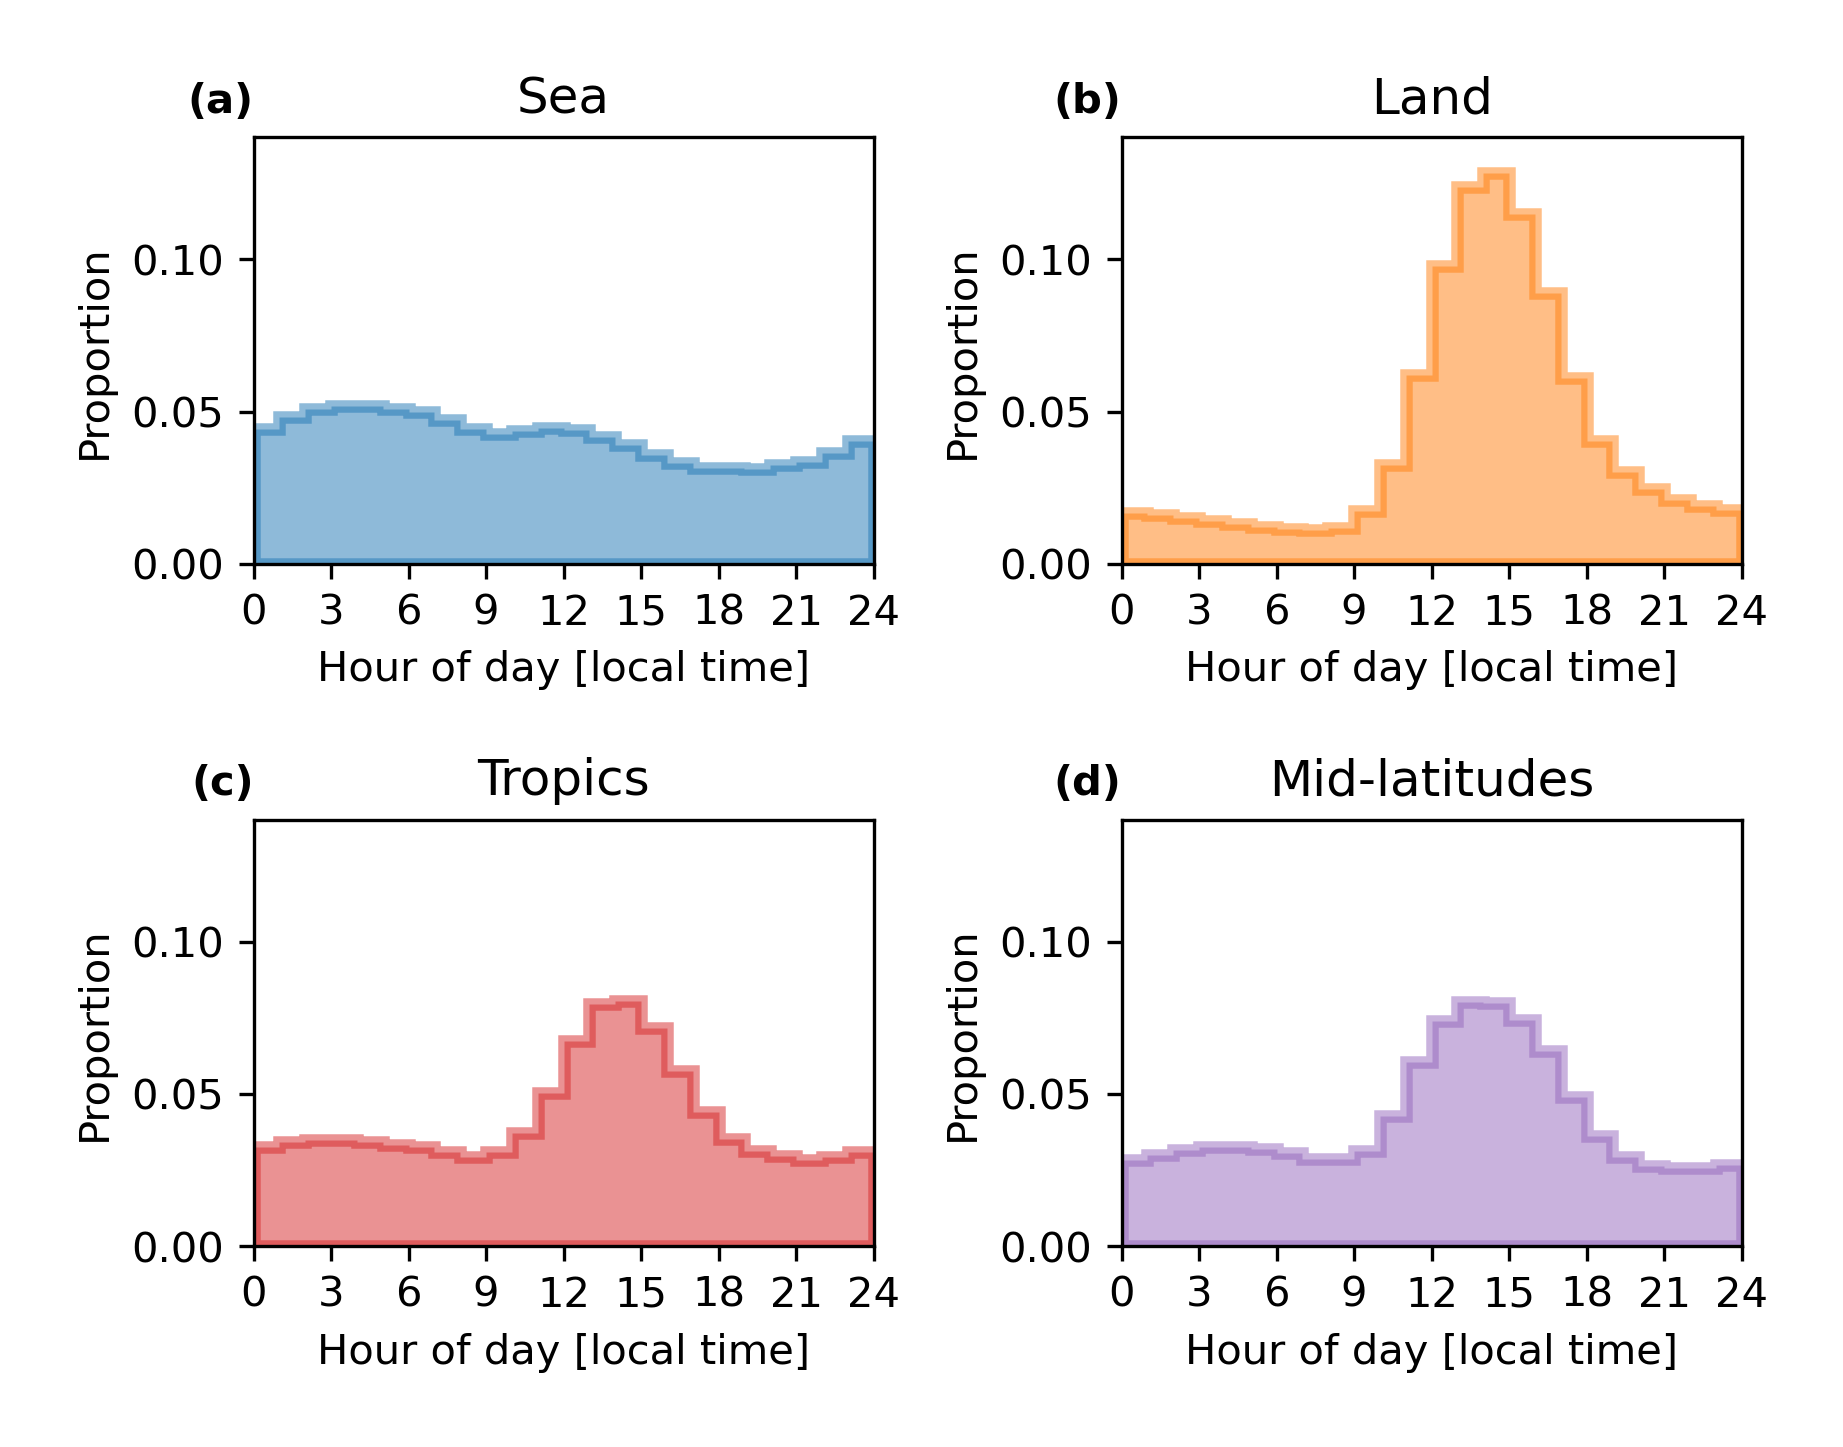
\includegraphics[width=\textwidth]{figures/chapter2_12.png}
    \caption[
    The diurnal distributions of the local time of detection for cores detected over land, sea, tropics and mid-latitudes
    ]{
    The diurnal distributions of the local time of detection for cores, binned by hour detected over (a) sea, (b) land, (c) tropics (\textless 30\,\textdegree N) and (d) mid-latitudes (\textgreater 30\,\textdegree N).
    }
    \label{fig:core_diurnal_land_sea}
\end{figure}


Figure~\ref{fig:core_diurnal_land_sea} shows the distribution of core detections across the diurnal cycle for land, sea, tropics and mid-latitude regions.
Over land there is a sharp peak in convective activity initiating in the mid-afternoon between 2 and 3 pm, with a tail extending into the night-time.
Over the sea, the distribution of core detections is much more uniform across the diurnal cycle.
There is still a peak observed in the early hours of the morning (3--6\,am), and a low in the evening (6\,pm), but the difference between these is much less pronounced than that over land.
Both the tropics and mid-latitudes have peaks in convection at the same time as that seen for all land regions in fig.~\ref{fig:core_diurnal_land_sea}\,b.
The peak for mid-latitudes is slightly broader however, with more convection occurring later in the day.

%f
\begin{figure}[tp]
    \centering
    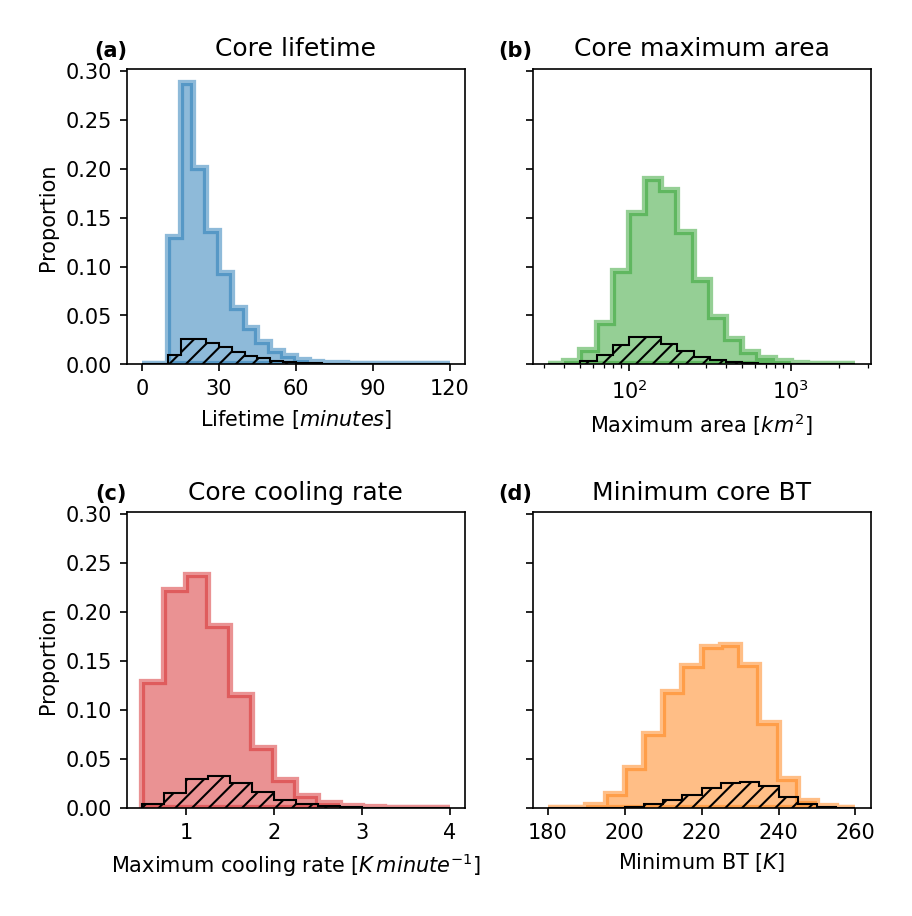
\includegraphics[width=0.75\textwidth]{figures/chapter2_13.png}
    \caption[
    The diurnal distribution of cores detected in the \acrshort{ngp} region
    ]{
    The diurnal distribution of cores detected in the \acrshort{ngp} region (37--45\,\textdegree\,N, 90--100\,\textdegree\,W).
    }
    \label{fig:core_ngp_contrast}
\end{figure}

Figure~\ref{fig:core_detection_time_map} showed a noticeably later average time of detection over the \acrfull{ngp} region.
Figure~\ref{fig:core_ngp_contrast} shows how the diurnal distribution of core detection time varies within this area, which is defined as 37--45\,\textdegree\,N, 90--100\,\textdegree\,W.
In contrast to the distribution seen over all land regions in fig.~\ref{fig:core_diurnal_land_sea}\,b, the \acrshort{ngp} region shows a later peak of convective activity between 3 and 4 pm, as well as much higher rates of convection observed during the nighttime and into the early morning until around 7\,am.
Previous studies have found a similar bimodal distribution in convective precipitation over the \acrshort{ngp} \citet{li_high-resolution_2021}.

%f
\begin{figure}[tp]
    \centering
    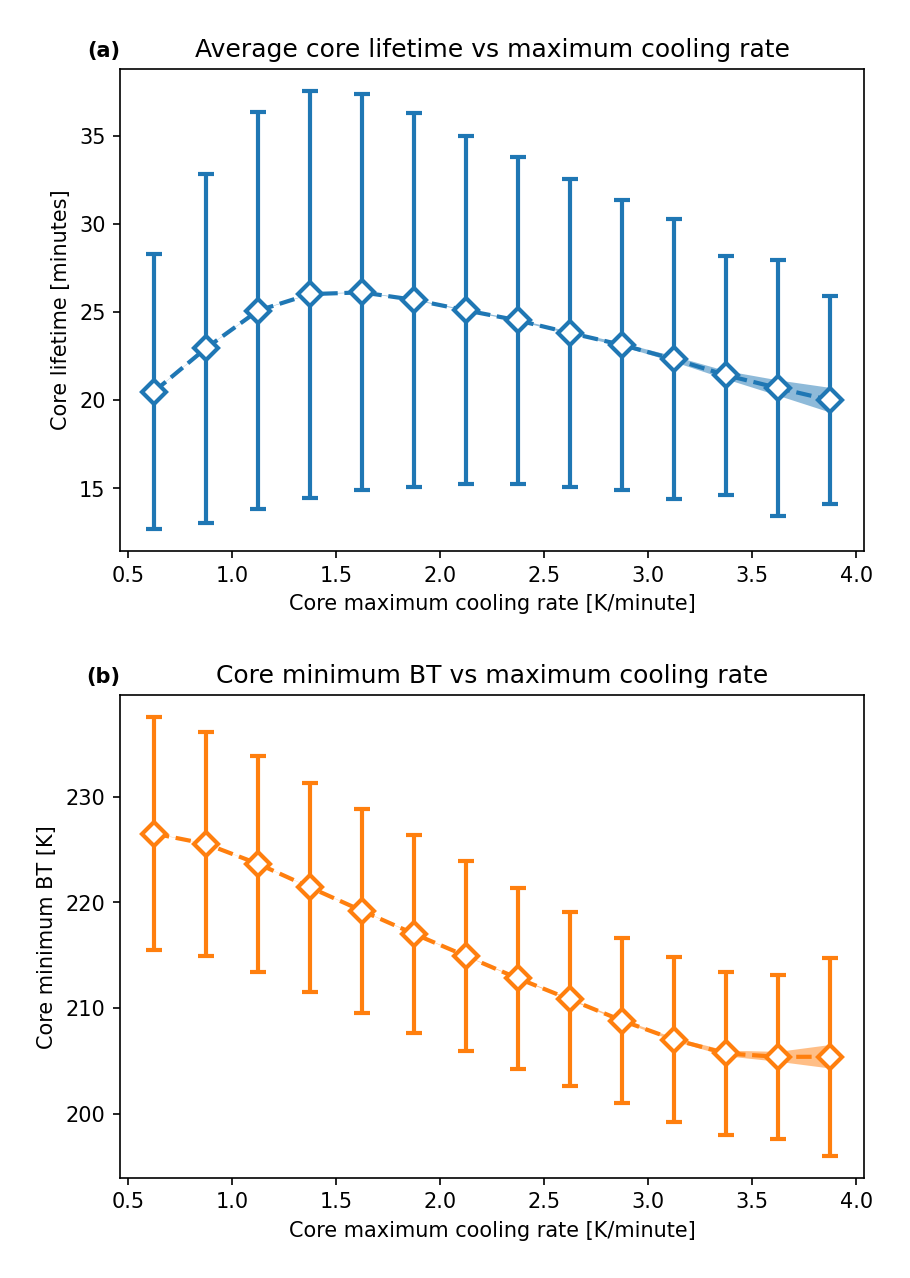
\includegraphics[width=0.75\textwidth]{figures/chapter2_14.png}
    \caption[
    The change in average time of core detection with distance from the coastline
    ]{
    The change in average time of core detection with distance from the coastline. Negative distances along the x axis show cores detected further to sea, and positive distances show cores detected further inland. Error bars show the circular standard deviation of the local solar hour of detection.
    }
    \label{fig:core_coast_effect}
\end{figure}

In fig.~\ref{fig:core_coast_effect} the effect of the distance to the coast on core detection time is examined over the Gulf Coast region (22.5--32.5\,\textdegree\,N, 82.5--100\,\textdegree\,W).
Negative distances indicate locations further offshore, and positive distances those locations further inland.
Figure~\ref{fig:core_detection_time_map} showed a change in the average time of detection of cores in locations closer to the coast, and that effect is shown again here.
For cores detected over the sea, there is a linear decrease in the average time of detection as the distance to the coast increases.
For cores detected over land, there is a sharp decrease in the time of detection very close to the coast, although further than 50\,\unit{km} from the coast this becomes a shallower linear gradient.
The linear change of core detection time with distance from the coastline may be linked to offshore and onshore breezes triggering convection.
Cores over land see a reduction in the variance of the time of detection between 50 and 150\,\unit{km} from the coast, which may also indicate that an external forcing from sea breeze is triggering convection in these areas, constraining the time of initiation of convection.

%f
\begin{figure}[tp]
    \centering
    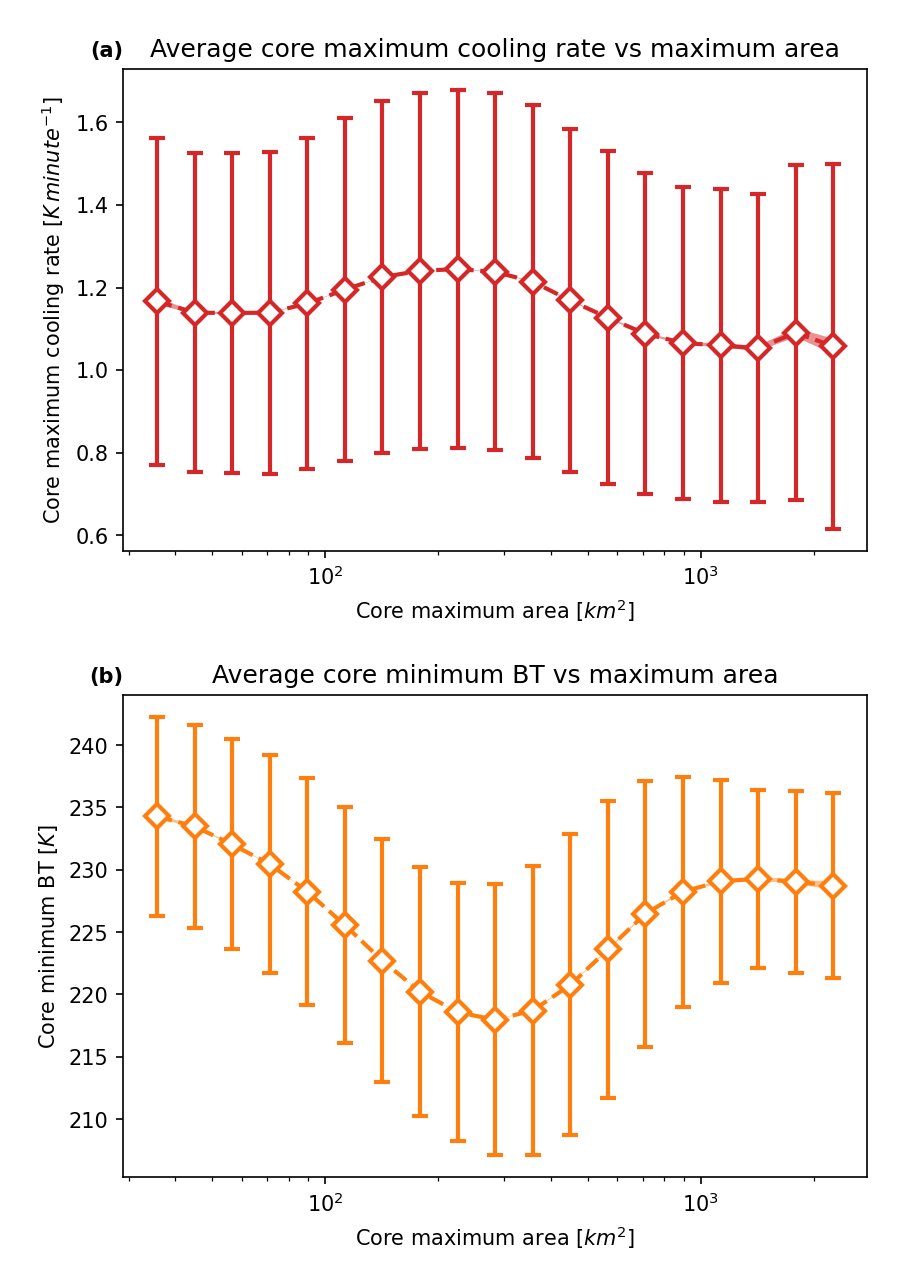
\includegraphics[width=\textwidth]{figures/chapter2_15.png}
    \caption[
    The diurnal cycle of the maximum cooling rate of cores detected over land, sea, tropics and mid-latitudes
    ]{
    The diurnal cycle of the maximum cooling rate of cores detected over (a) sea, (b) land, (c) tropics (\textless 30\,\textdegree N) and (d) mid-latitudes (\textgreater 30\,\textdegree N). Each point shows the mean of the maximum cooling rate of cores detected during that hour. Error bars show the standard deviation of maximum cooling rate.
    }
    \label{fig:core_diurnal_cooling_rate}
\end{figure}

Figure~\ref{fig:core_diurnal_land_sea} shows how the mean maximum cooling rate of cores changes across the diurnal cycle.
While over sea there is little change in cooling rate, over land there is a noticeable increase in the cooling rate throughout the daylight hours.
This leads to a peak at around 4\,pm, before cooling rate falls back to its nighttime levels which are lower than that seen over ocean.
Both tropics and mid-latitudes show similar diurnal cycles to land, albeit with a difference of 0.2\,\unit{K minute\textsuperscript{-1}} across the entire diurnal cycle.


\subsection{Distributions and properties of observed anvil clouds} \label{sec:anvil_properties}

In this section, the properties of anvil clouds in the dataset are examined.
Anvils are detected and tracked independently from cores.
Although anvils must be associated with observed cores at the start of their lifetime, tracking of anvils continues beyond the extent of the observed core lifetime.
This also allows the detection of anvils that are associated with multiple cores, providing insight into the effects of convective organisation on anvil properties.

%f
\begin{figure}[tp]
    \centering
    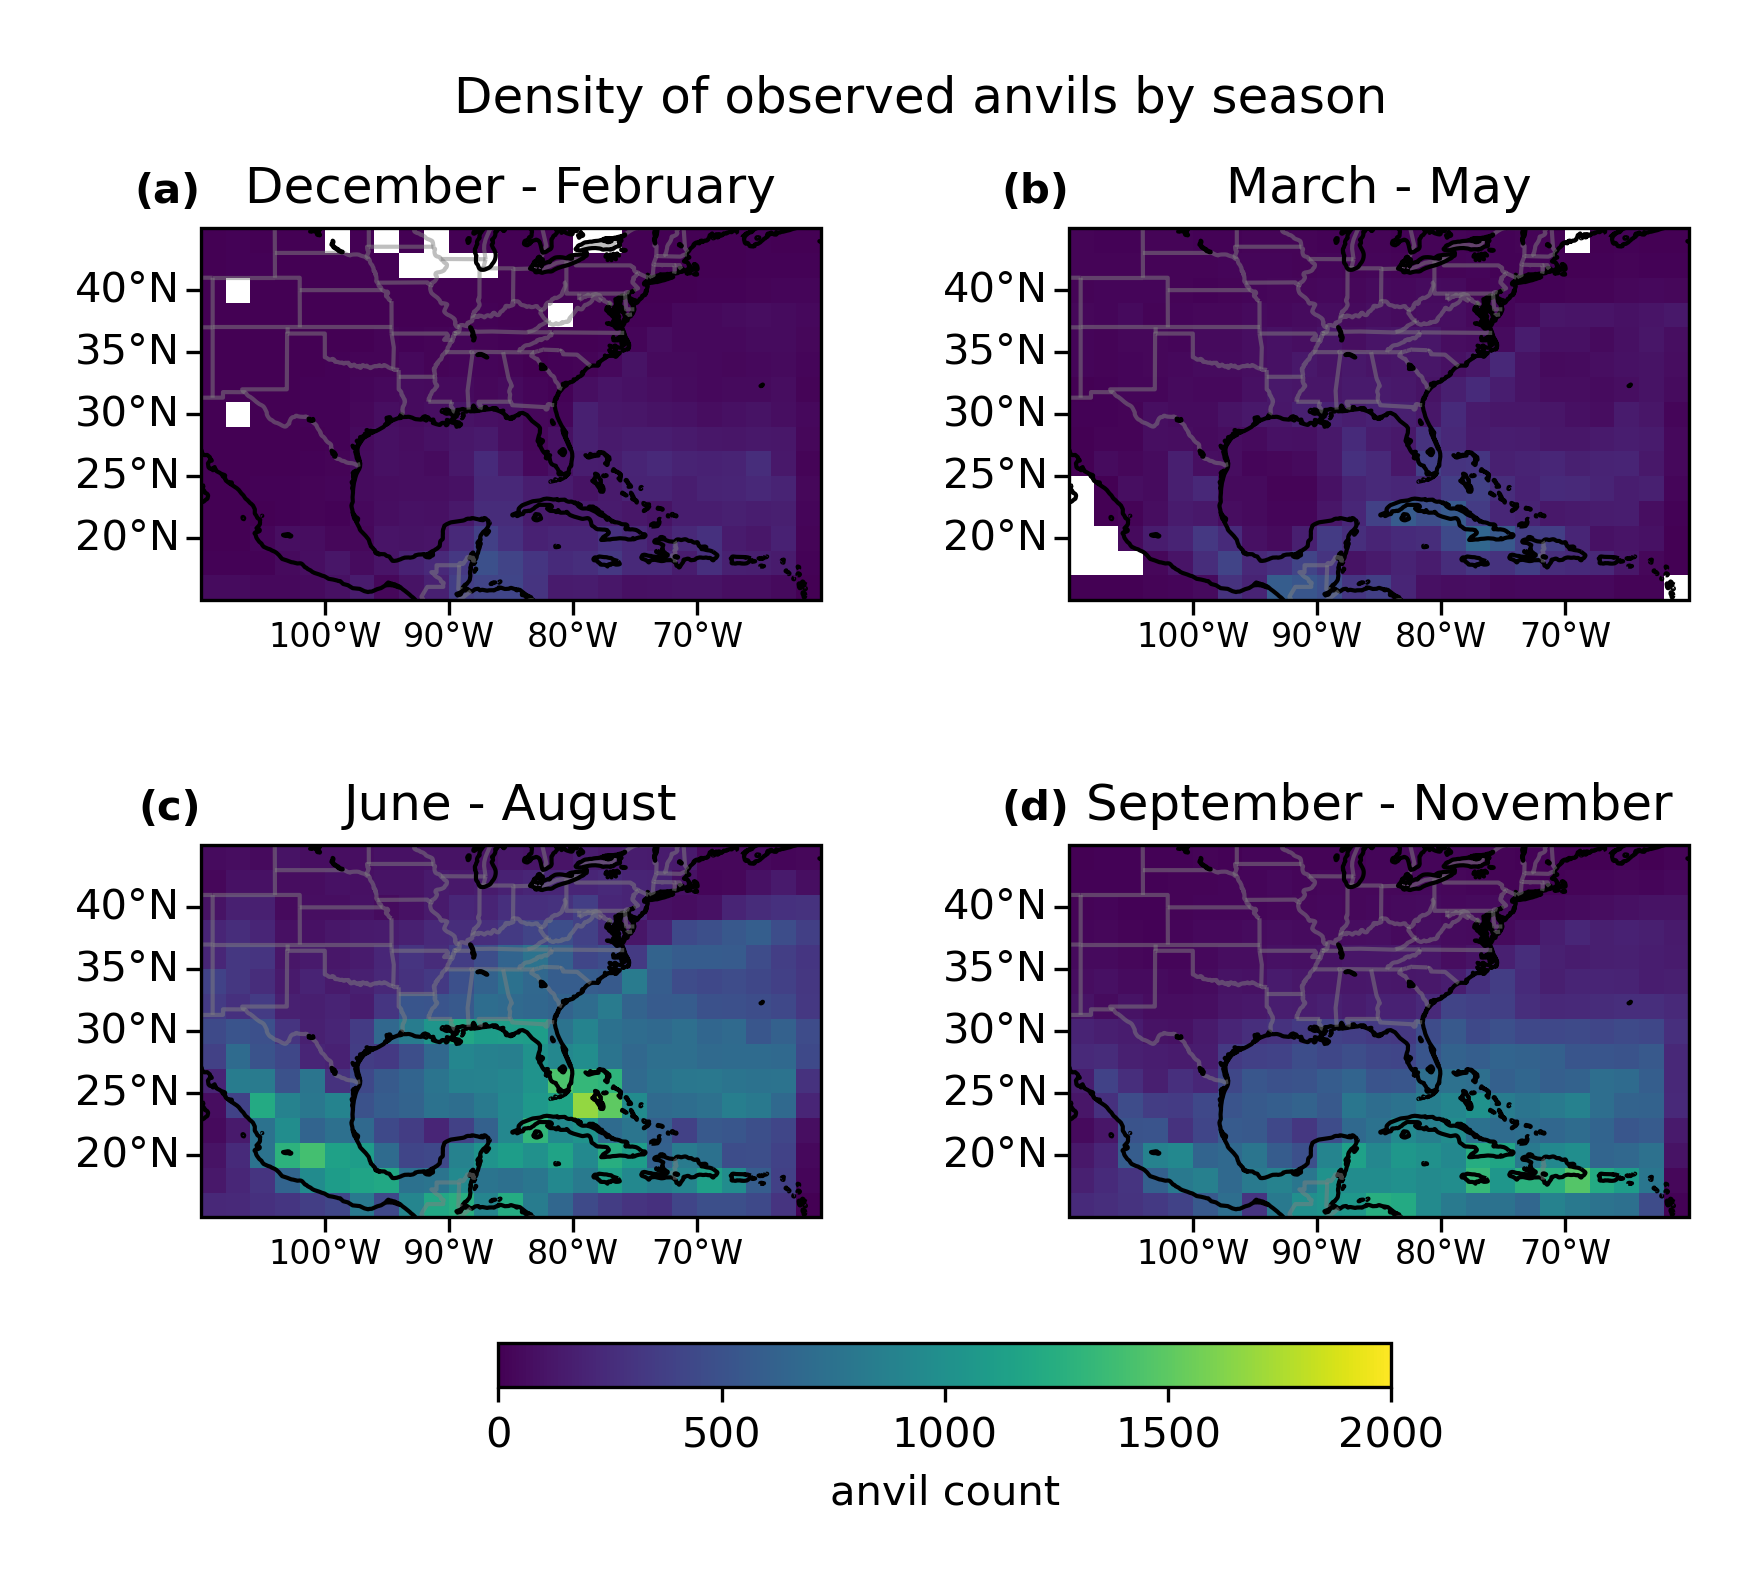
\includegraphics[width=\textwidth]{figures/chapter2_16.png}
    \caption[
    Maps showing the spatial distribution of observed anvils by season
    ]{
    Maps showing the spatial distribution of observed anvils for (a) winter, (b) spring, (c) summer and (d) autumn, each binned to a 2\texttimes2\,\textdegree grid.
    }
    \label{fig:anvil_distribution_map}
\end{figure}

Figure~\ref{fig:anvil_distribution_map} shows the counts of anvils for each 2\texttimes2\,\textdegree grid box, separated by season.
There is a similar seasonal cycle and distribution to fig.~\ref{fig:core_density_by_season}.
In winter (fig.~\ref{fig:anvil_distribution_map}\,a) and spring (fig.~\ref{fig:anvil_distribution_map}\,b) there are low rates of convection, with the majority of convection observed over warm ocean regions.
In summer, fig.~\ref{fig:anvil_distribution_map}\,c shows the highest rates of anvil detections, with a large increase in the observations of anvils over land.
In spring (fig.~\ref{fig:anvil_distribution_map}\,d), the number of anvils observed over the ocean remains high, but that over land reduces.

%f
\begin{figure}[tp]
    \centering
    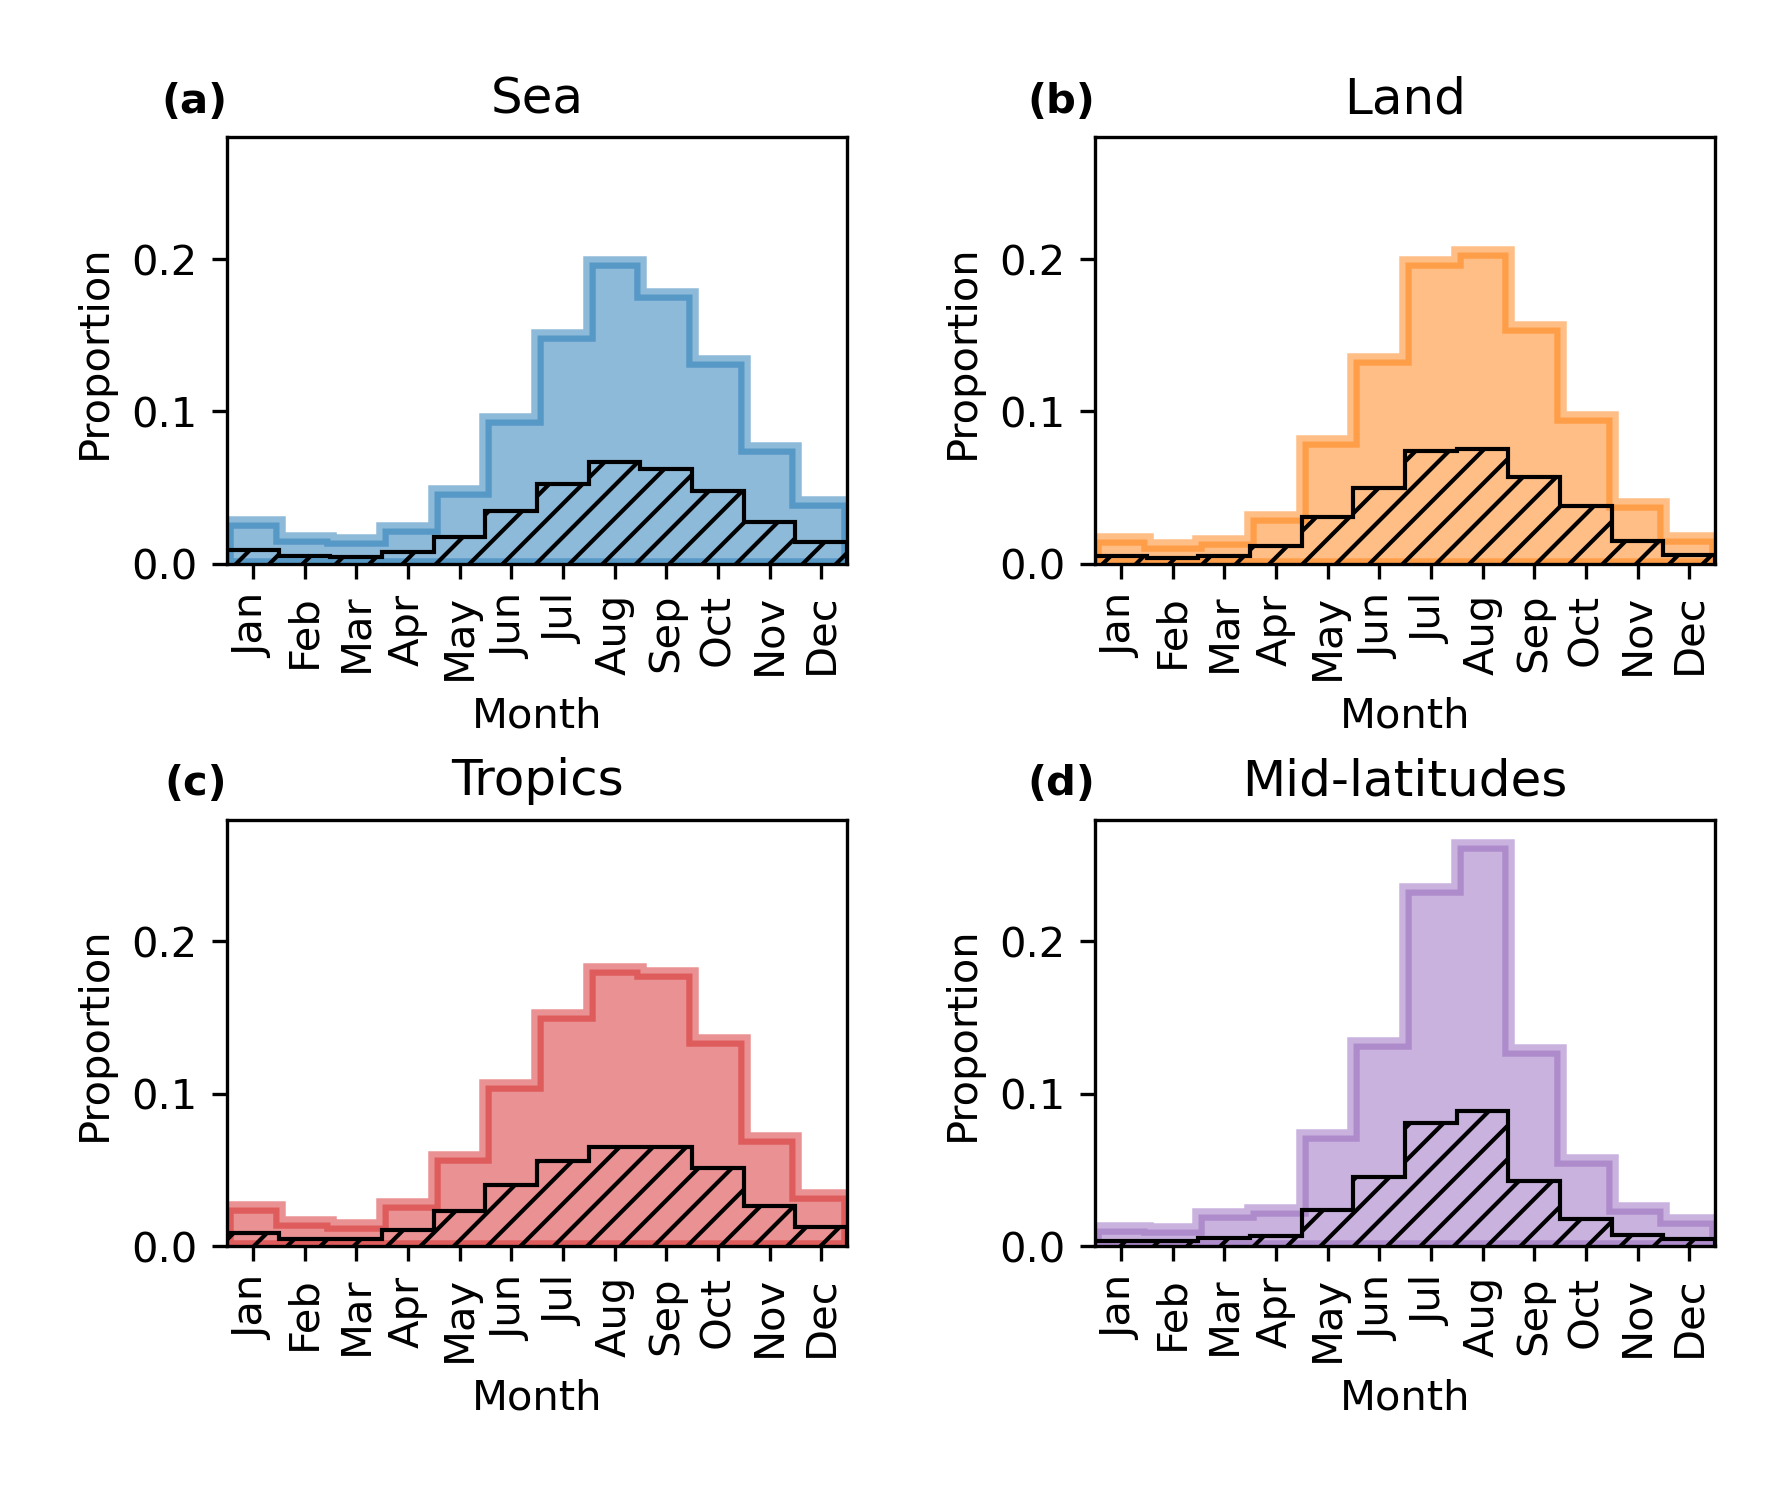
\includegraphics[width=\textwidth]{figures/chapter2_17.png}
    \caption[
    Monthly distributions of the proportion of cores detected each month over land, sea, tropics and mid-latitudes
    ]{
    Monthly distributions of the proportion of cores detected each month over (a) sea, (b) land, (c) tropics (\textless 30\,\textdegree N) and (d) mid-latitudes (\textgreater 30\,\textdegree N). The hatched area shows the proportion of the distribution consisting of anvils with multiple cores.
    }
    \label{fig:anvil_monthly_cycles}
\end{figure}

Figure~\ref{fig:anvil_monthly_cycles} shows how the annual distribution of anvil detections changes by month across different regions.
Similarly to the annual distribution of cores shown in fig.~\ref{fig:core_annual_land_sea} shows a later peak over oceans in August--September compared to July--August over land.
The mid-latitudes have a sharper peak around these two months, while the tropics show a broader distribution of anvil detections throughout the year.


%f
\begin{figure}[tp]
    \centering
    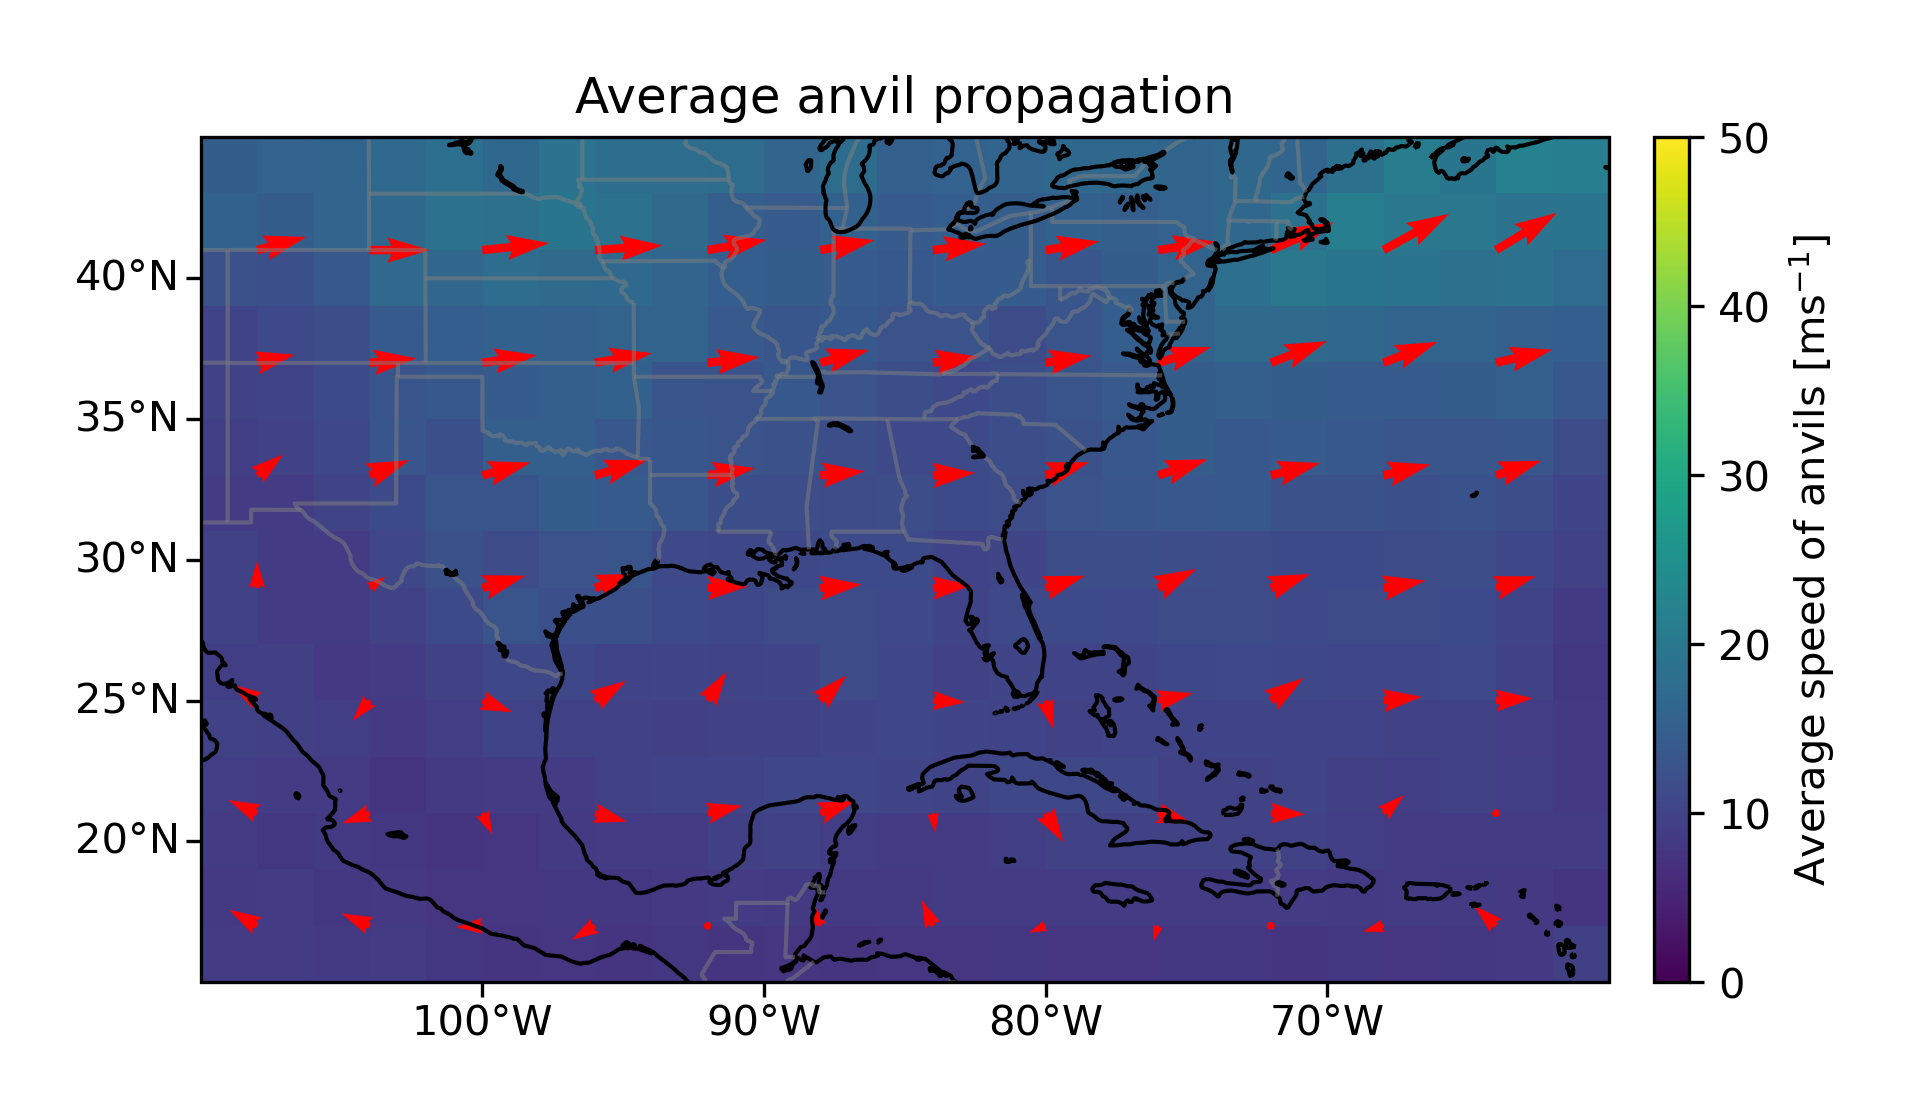
\includegraphics[width=\textwidth]{figures/chapter2_18.png}
    \caption[
    The average speed and direction of propagation of anvils
    ]{
    The average speed and direction of propagation of cores observed within each 2\texttimes2\textdegree\ grid box. The colouring shows the average speed of propagation, and the red arrows show the average direction of propagation for each 4\texttimes4\textdegree\ grid box
    }
    \label{fig:anvil_propagation_map}
\end{figure}

Figure~\ref{fig:anvil_propagation_map} shows the average propagation speed and direction for anvils in the same manner as shown for cores in fig.\ref{fig:core_propagation_map}.
In the extra-tropics (\textgreater30\,\textdegree\,N), there is generally a westerly motion, without the southerly motion seen in the cores.
This westerly motion corresponds to the prevailing high-level winds.
The change in direction and differences in the speed of propagation between anvils and cores indicates a typical shear between the two.
Over the tropics (\textless30\,\textdegree\,N) no clear overall motion of anvils is apparent.


%f
\begin{figure}[tp]
    \centering
    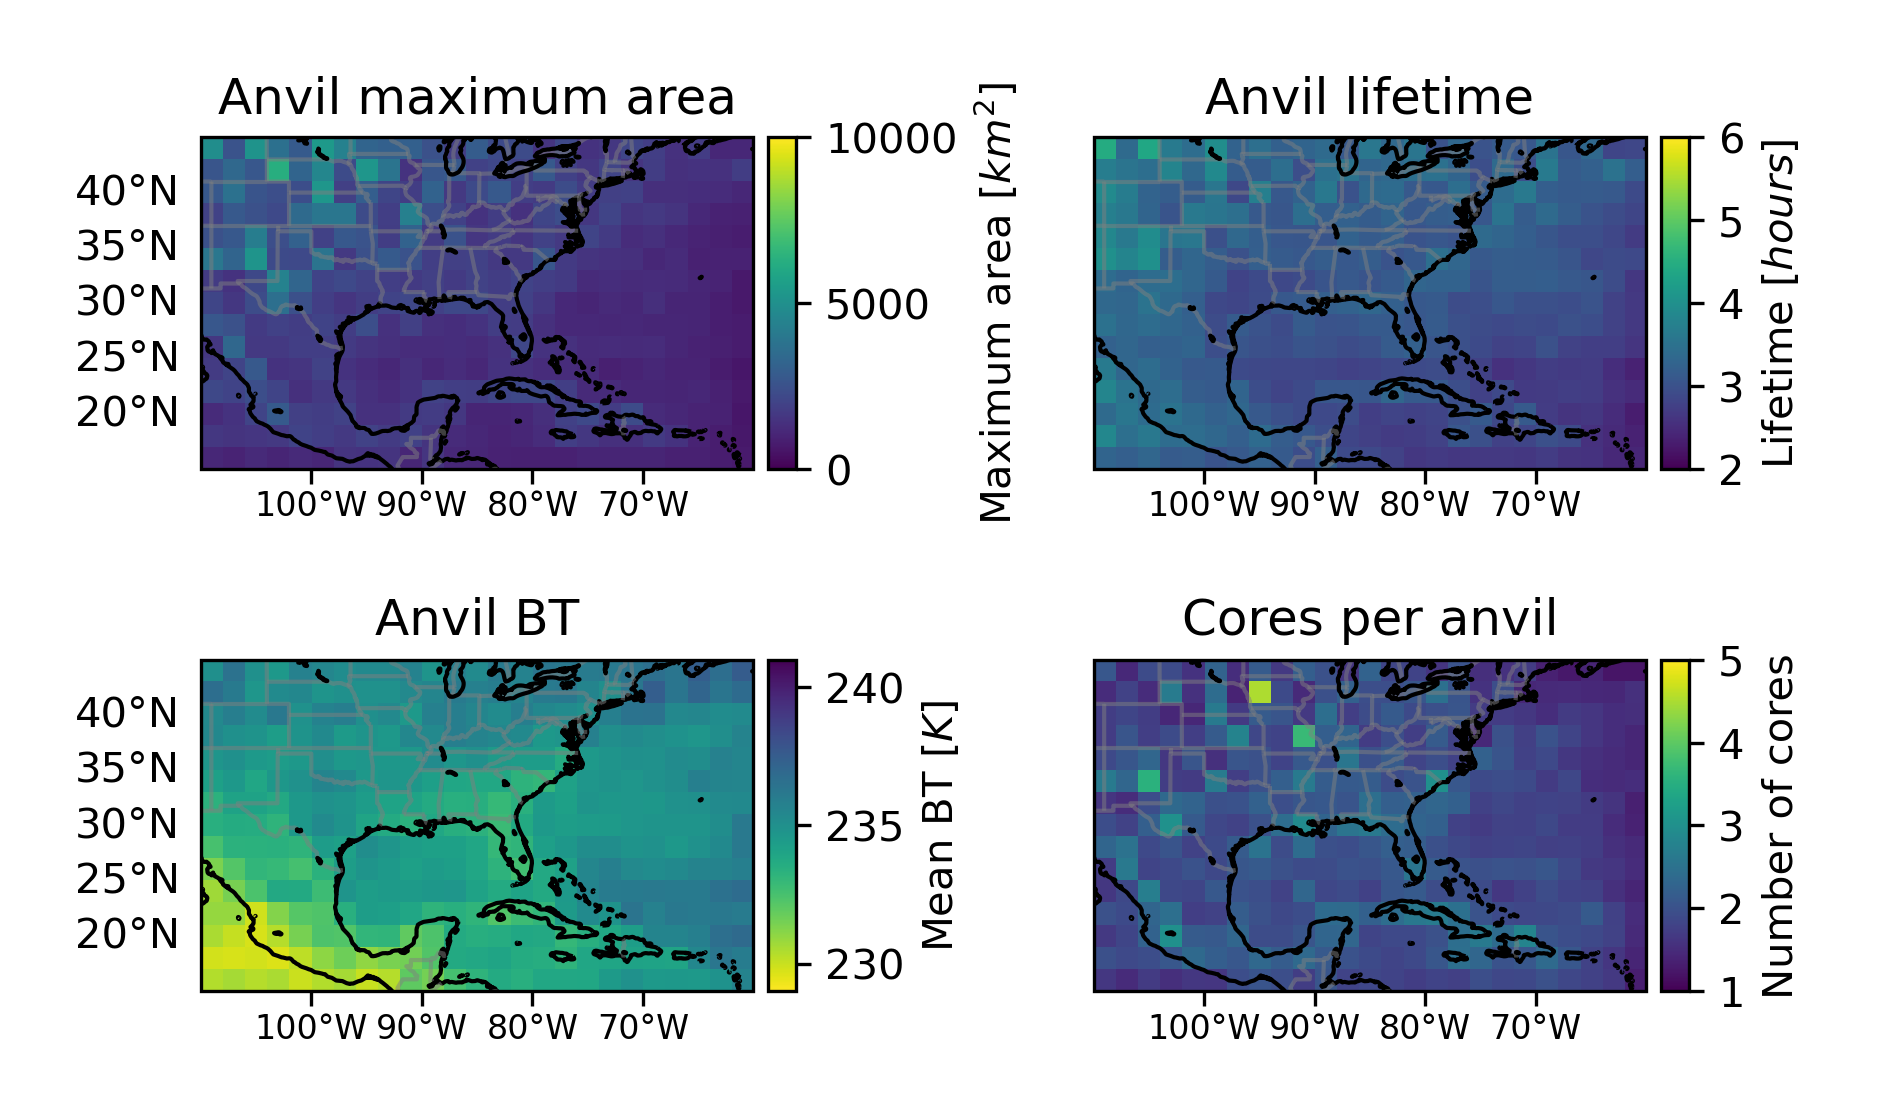
\includegraphics[width=\textwidth]{figures/chapter2_19.png}
    \caption[
    Maps showing the spatial changes in the averages of anvil maximum area, lifetime, \acrshort{bt} and number of cores
    ]{
    Maps showing the spatial changes in the averages of (a) anvil maximum area, (b) lifetime, (c) \acrshort{bt} and (d) number of cores, binned to a 2\texttimes2\,\textdegree grid.
    }
    \label{fig:anvil_properties_maps}
\end{figure}

Figure~\ref{fig:anvil_properties_maps}\,a shows the average maximum area of anvils for each 2\texttimes2\,\textdegree grid box.
There is again a land--sea contrast in the Caribbean and Gulf of Mexico.
The most notable change is the increase in anvil area towards the North--West of the domain.
This correlates with the change in sensor zenith angle---and hence the area of each pixel---shown in fig.~\ref{fig:abi_zenith_angles}.
It is possible that there is a bias towards observing larger anvils due to the larger pixel area at larger zenith angles.
However, previous studies have shown that this region is where most \acrshort{mcs}s in North America originate from \citep{feng_spatiotemporal_2019} which may also explain the large average areas.

Figure~\ref{fig:anvil_properties_maps}\,b shows the average anvil lifetime (in hours) for each 2\texttimes2\,\textdegree grid box.
There is a similar, but smaller, trend towards longer-lived anvils in the North-West of the domain as that seen for the anvil area in fig.~\ref{fig:anvil_properties_maps}\,a.
In addition, there is a tendency for average lifetimes over the ocean to be shorter than adjacent land regions.

Figure~\ref{fig:anvil_properties_maps}\,c shows the average \acrshort{bt} of anvils in each grid box.
Increasing latitude shows an increase (warming) of \acrshort{bt} over land.
In addition, there is a land--sea contrast, with warmer \acrshort{bt} over sea than land.
The coldest average \acrshort{bt} are observed over the Western coast of Mexico.

Figure~\ref{fig:anvil_properties_maps}\,d shows the average number of cores associated with each anvil in each grid box.
The Caribbean shows a noticeable land--sea contrast with an increase in the average number of cores over land, indicating that there is greater organisation of convection occurring there compared to over the sea.
For the majority of land regions the average is reasonably noisy.
This is primarily due to the presence of a small number of very large systems (including \acrshort{mcs}s), which have a very large number of cores and hence introduce noise to the spatial average.
In addition, there is see a reduction in the average number of cores towards the edge of the map which is likely due to larger anvils being more likely to be removed from the dataset by the criteria in table~\ref{table:anvil_validity_criteria}.

%f
\begin{figure}[tp]
    \centering
    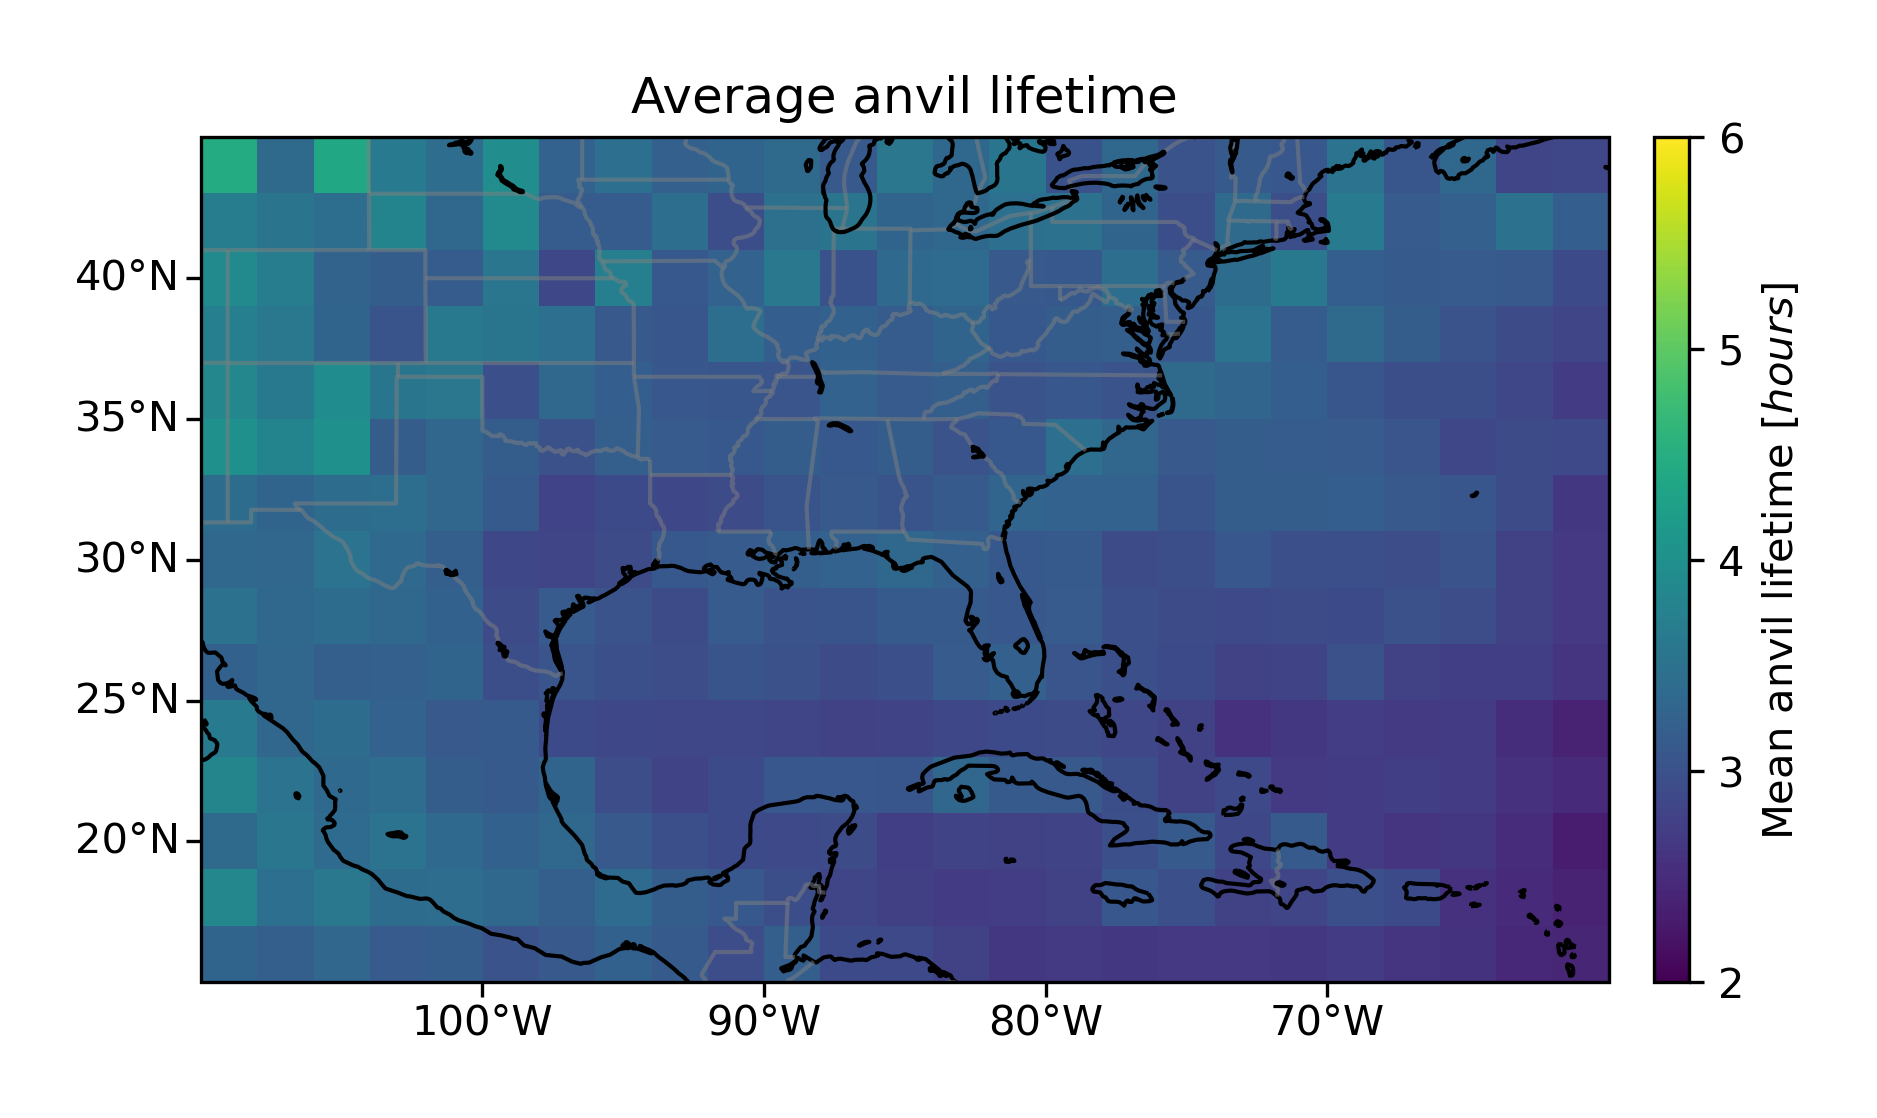
\includegraphics[width=0.9\textwidth]{figures/chapter2_20.png}
    \caption[
    Histograms showing the distribution of observed anvil properties
    ]{
    Histograms showing the distribution of observed anvil properties, with the hatched area showing the proportion associated with multiple core anvils. (a) The maximum area of the thick anvil cloud; (b) the maximum area of the thin anvil cloud (which includes both the thick and thin anvil regions; (c) the lifetime of the thick anvil and (d) the thin anvil; and (e) the average and (f) minimum observed \acrshort{bt} within each anvil.
    }
    \label{fig:anvil_properties}
\end{figure}

Figure~\ref{fig:anvil_properties} shows the distributions of anvil properties, with the proportion consisting of multiple-core anvils shown by the hatched area.
The anvil maximum area distribution has a similar shape for both thick anvils (fig.~\ref{fig:anvil_properties}\,a) and thin anvils (fig.~\ref{fig:anvil_properties}\,b), with the mean shifted to large values for the thin anvil.
It should be noted that the thin anvil area includes that of both thick and thin anvil regions, so will always be larger than that of the thick anvil alone.
The anvil lifetime distributions for the thick (fig.~\ref{fig:anvil_properties}\,c) and thin (fig.~\ref{fig:anvil_properties}\,d) anvils show a similar relationship, with a shift of the distribution to longer lifetimes for the thin anvil.
In both cases, despite the log scaling on the x-axis, there is a long tail towards larger area values and longer lifetimes.
Furthermore, this large tail consists primarily of multiple-core systems, as shown by the hatched area, indicating the impact of organisation on the area and lifetime of \acrshort{dcc}s.

Figure~\ref{fig:anvil_properties}\,e and fig.~\ref{fig:anvil_properties}\,f show the average and minimum anvil \acrshort{bt} over each detected anvil.
The minimum anvil \acrshort{bt} has a broader distribution than that of the average anvil \acrshort{bt}.
Multiple core anvils generally have colder anvil \acrshort{bt}, particularly so for the minimum \acrshort{bt}.
The cold tail of the minimum \acrshort{bt}, with values less than 200\,\unit{K}, indicates the presence of overshooting tops within these organised systems.

%f
\begin{figure}[tp]
    \centering
    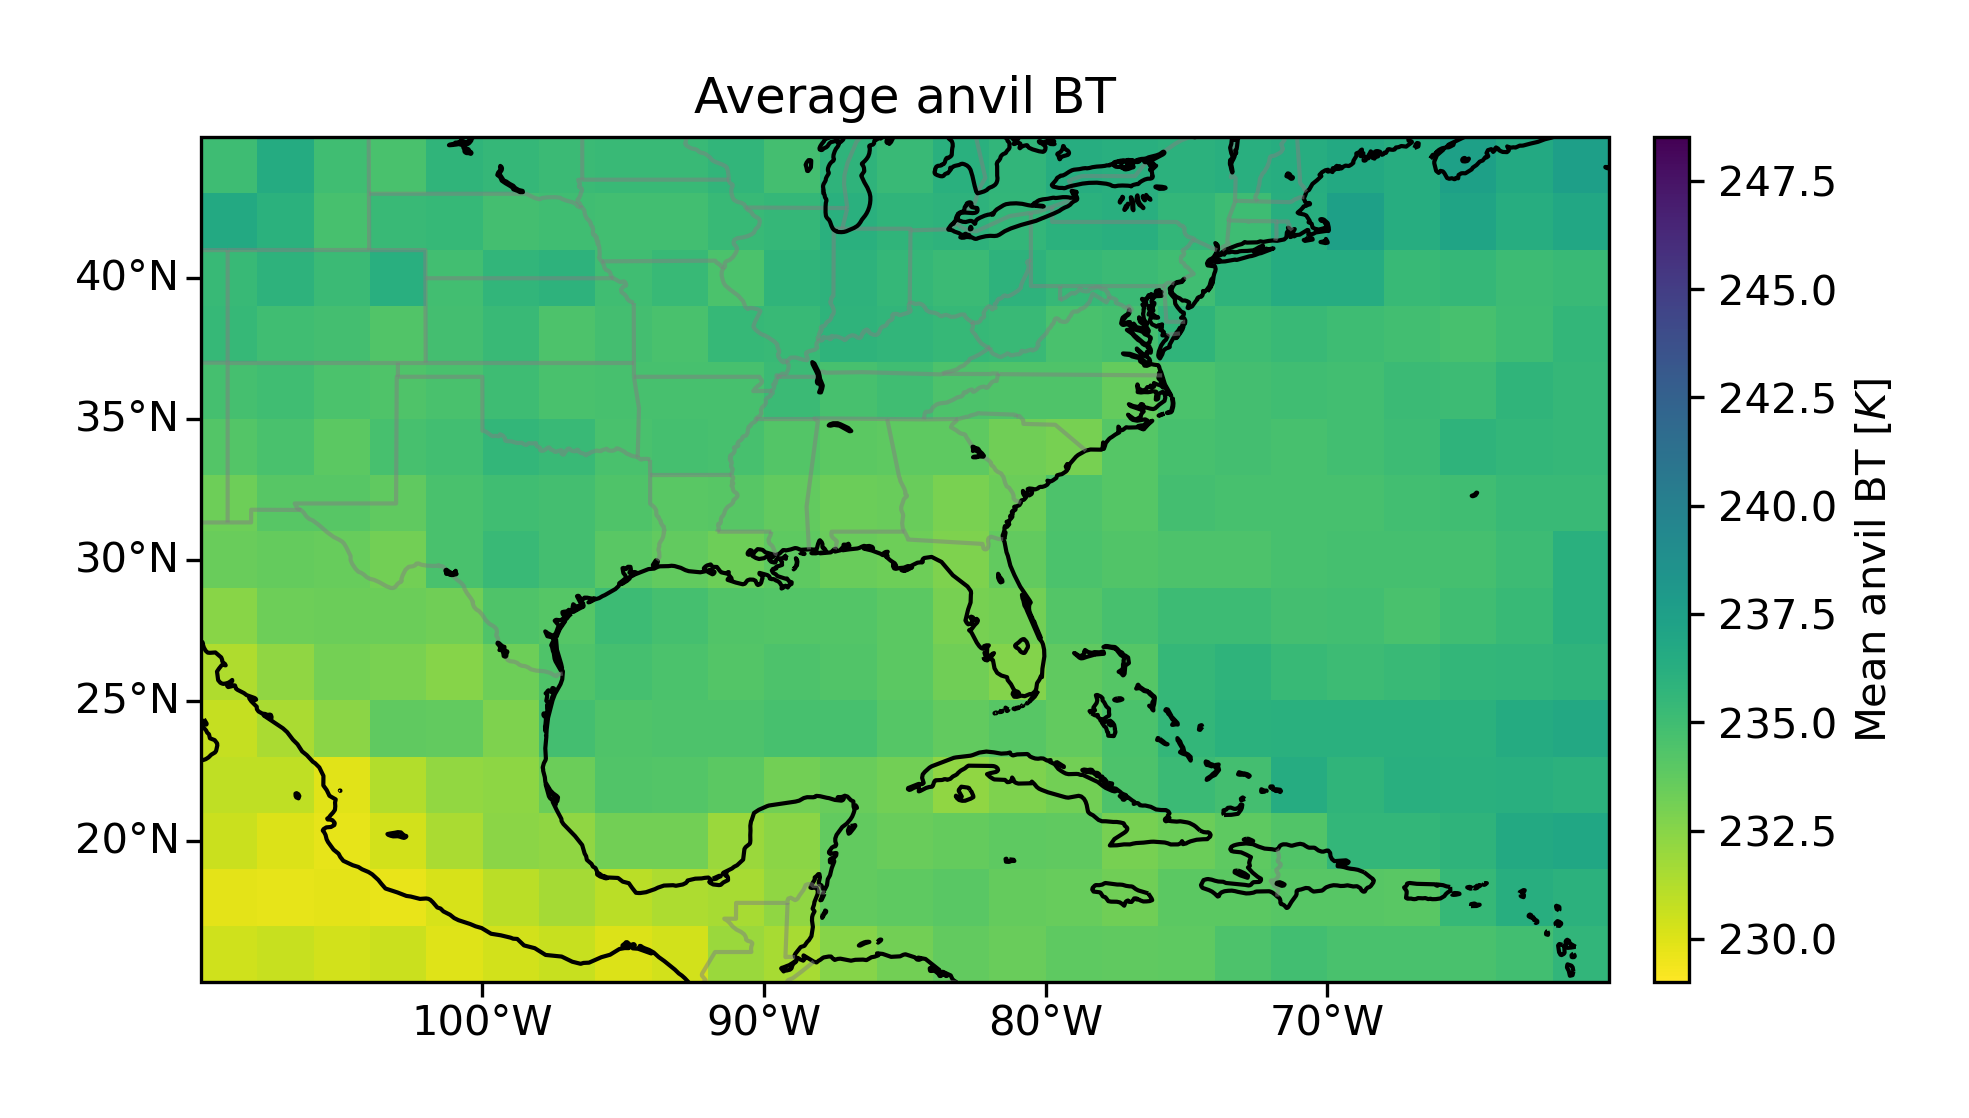
\includegraphics[width=0.9\textwidth]{figures/chapter2_21.png}
    \caption[
    The change in the average area and lifetime of anvils with different number of cores, and their total area coverage.
    ]{
    The change in the average area and lifetime of anvils with different number of cores. Mean values of (a) maximum thick anvil area, (b) maximum thin anvil area, (c) thick anvil lifetime and (d) thin anvil lifetime all increase with increasing number of cores. (e) The proportion of all anvils with different numbers of cores and (f) the fraction of total anvil coverage attributed to those anvils.}
    \label{fig:anvil_cores_and_coverage}
\end{figure}

Figure~\ref{fig:anvil_cores_and_coverage}\,a, b, c and d the average of the thick anvil maximum area, thin anvil maximum area, thick anvil lifetime and thin anvil lifetime for anvils with different numbers of cores.
In all cases these areas and lifetimes increase with an increasing number of cores.
In particular, the increase in the number of cores has a large impact on the maximum area of anvils, 
The most organised systems, which contain 10 or more cores, have areas that are more than two orders of magnitude greater on average than the anvils of isolated \acrshort{dcc}s.

Figure~\ref{fig:anvil_cores_and_coverage}\,e and f show the distribution of the number of cores associated with each detected anvil, and the proportion of total anvil coverage attributed to anvils with different core counts respectively.
Overall, the vast majority of anvils detected are isolated \acrshort{dcc}s with only a single core.
For anvils with greater than five cores, the number of systems observed drops to such a level that grouping of these \acrshort{dcc}s into bins of 6--9 cores and 10 or more is performed to ensure that there is a representative sample size of each group.
Despite making up the majority of observed \acrshort{dcc}s, single core systems only make up 12\% of the total anvil coverage.
Instead, despite being few in number, it is the most organised \acrshort{dcc}s---those with ten or more cores---which are responsible for the majority of anvil coverage due to their large area and lifetime.
The large area and lifetime of these systems---seen in the long tails of those distributions in fig.~\ref{fig:anvil_properties}---compound to result in this large coverage.

%f
\begin{figure}[tp]
    \centering
    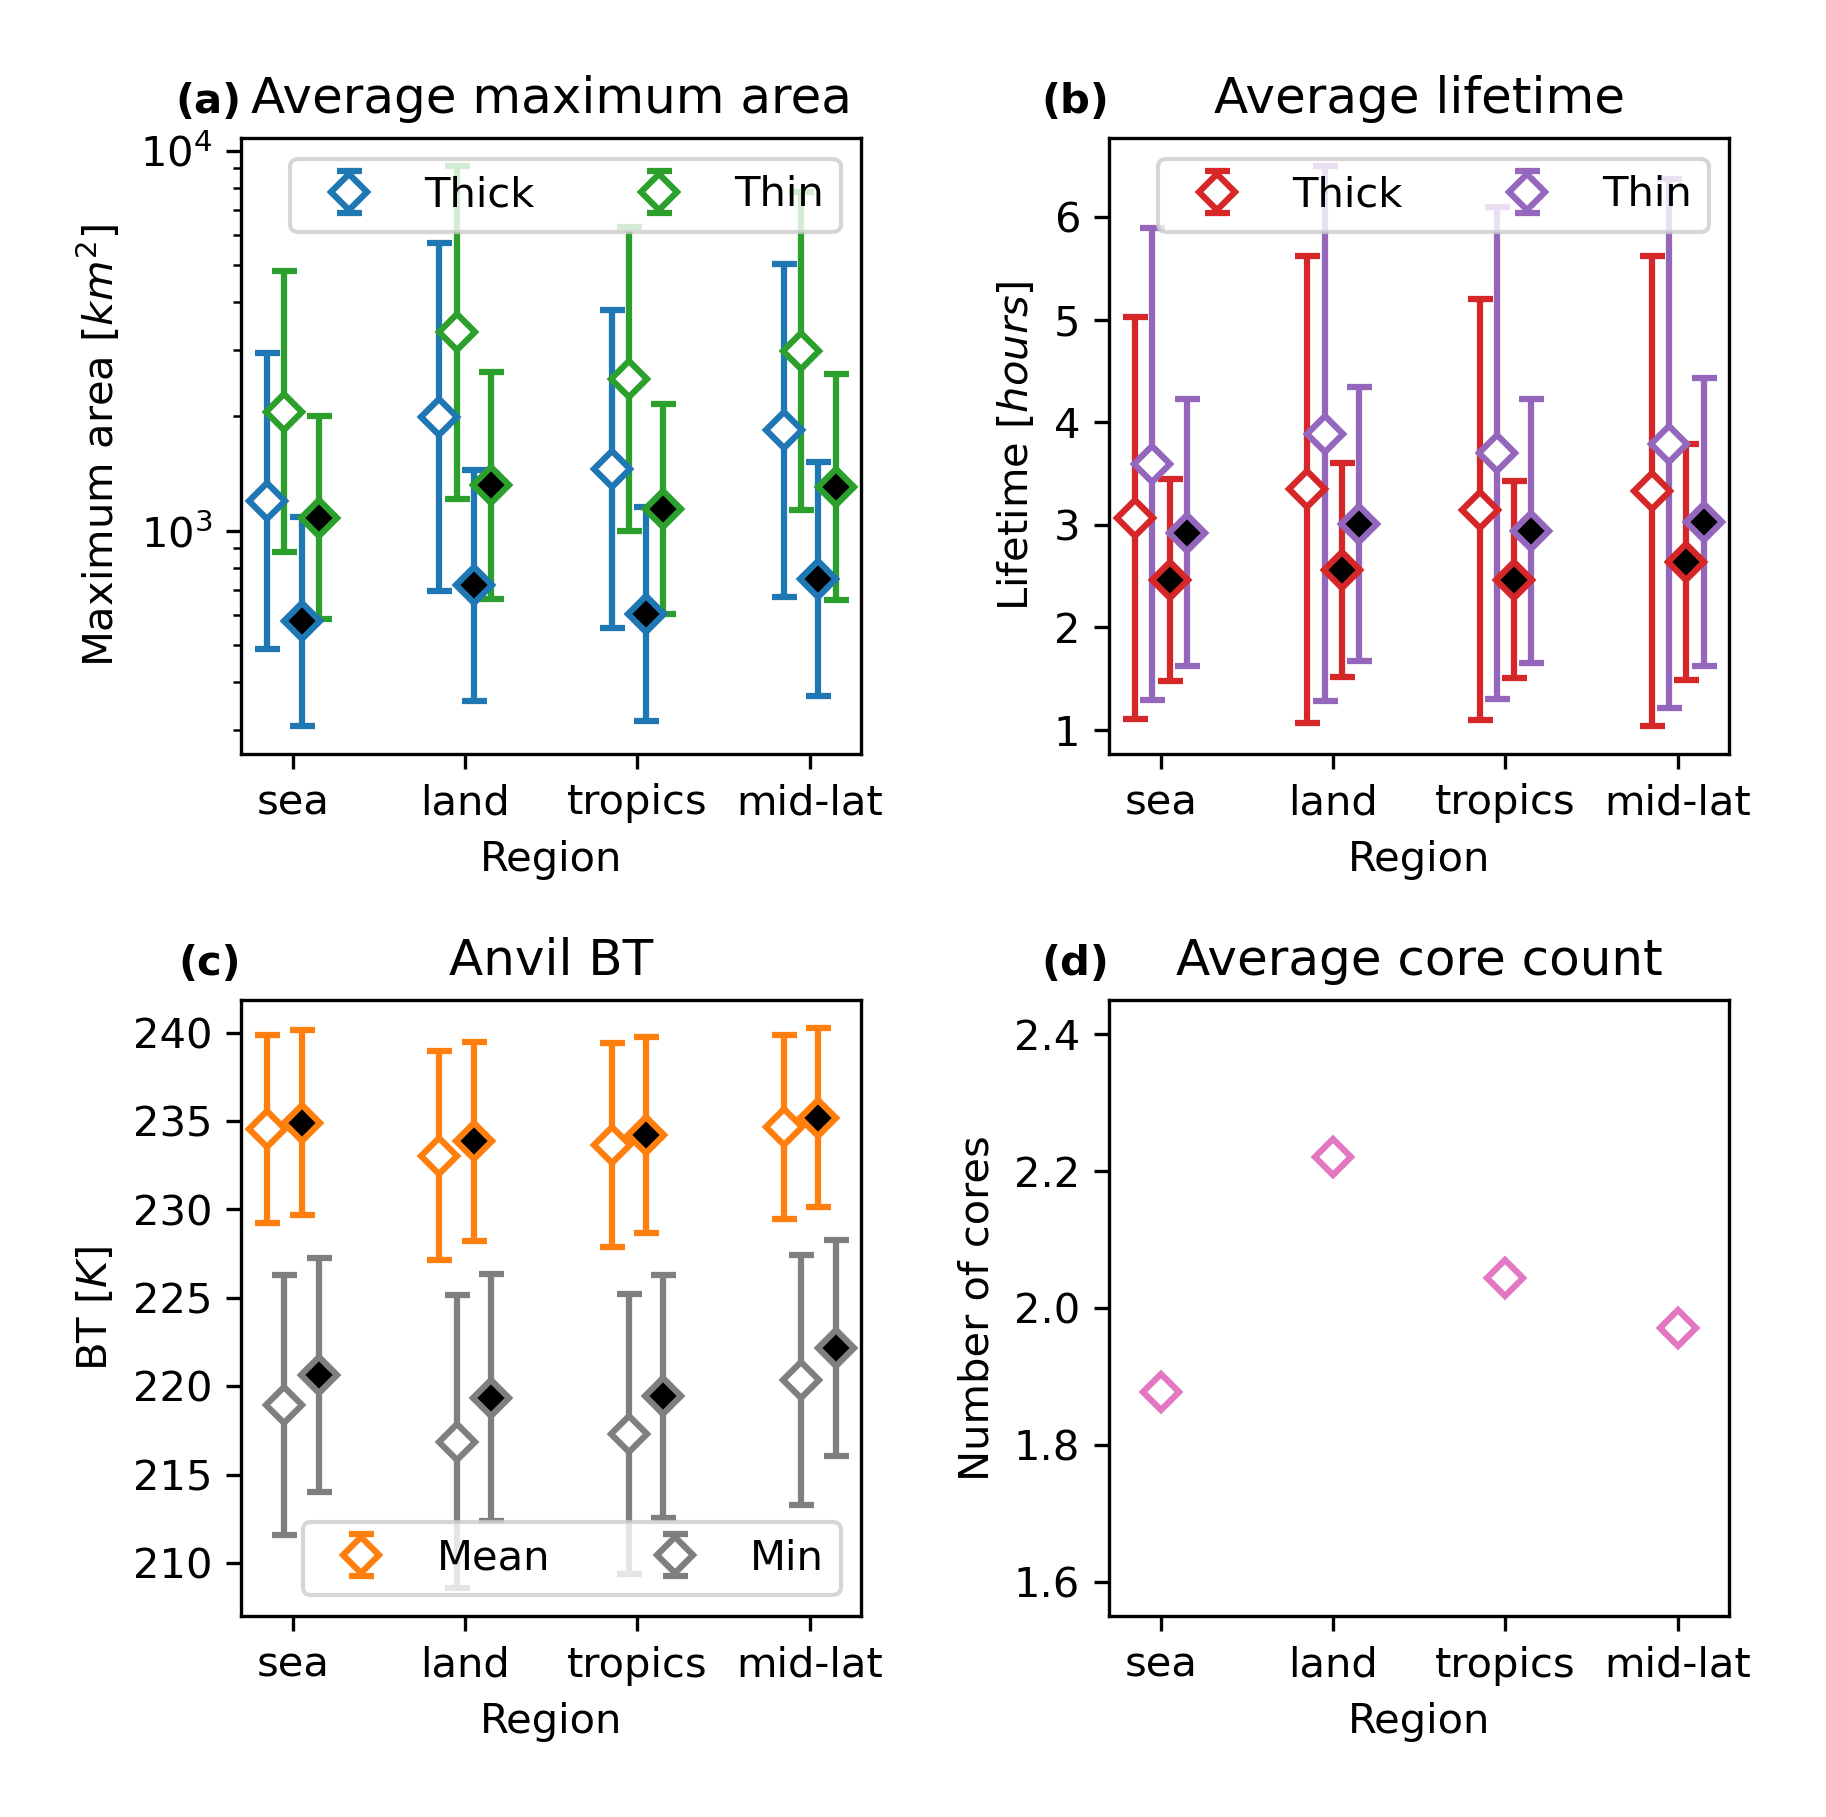
\includegraphics[width=0.9\textwidth]{figures/chapter2_22.png}
    \caption[
    The change in the average areas, lifetimes, \acrshort{bt} and number of cores of anvils observed over sea, land, tropics and mid-latitudes.
    ]{
    The change in the average (a) areas, (b) lifetimes, (c) \acrshort{bt} and (d) number of cores of anvils observed over sea, land, tropics and mid-latitudes. The points with no fill show the average across all \acrshort{dcc}s, whereas the points with the black fill show the average for isolated \acrshort{dcc}s (with one core) only. Error bars show the standard deviation on the mean.
    }
    \label{fig:anvil_properties_regions}
\end{figure}

Figure~\ref{fig:anvil_properties_regions} shows how the averages of the maximum areas, lifetimes, \acrshort{bt} and number of cores vary between different regions.
For both isolated and multi-core convection, the average areas and lifetimes shown in fig.~\ref{fig:anvil_properties_regions}\,a and b respectively are larger over land than sea, and in the mid-latitudes than in the tropics.
For the anvil \acrshort{bt} shown in fig.~\ref{fig:anvil_properties_regions}\,c, both the mean and minimum \acrshort{bt} of anvils is colder over land than sea, and also colder in the tropics than in the mid-latitudes.
\acrshort{dcc}s over land tend to have more cores than those over sea, however is is clear that as these differences also apply to isolated \acrshort{dcc}s, they are connected to changes in the convective processes and anvil evolution in the different regions, rather than simply a sampling bias.

\subsection{Diurnal cycle of anvils}

%f
\begin{figure}[tp]
    \centering
    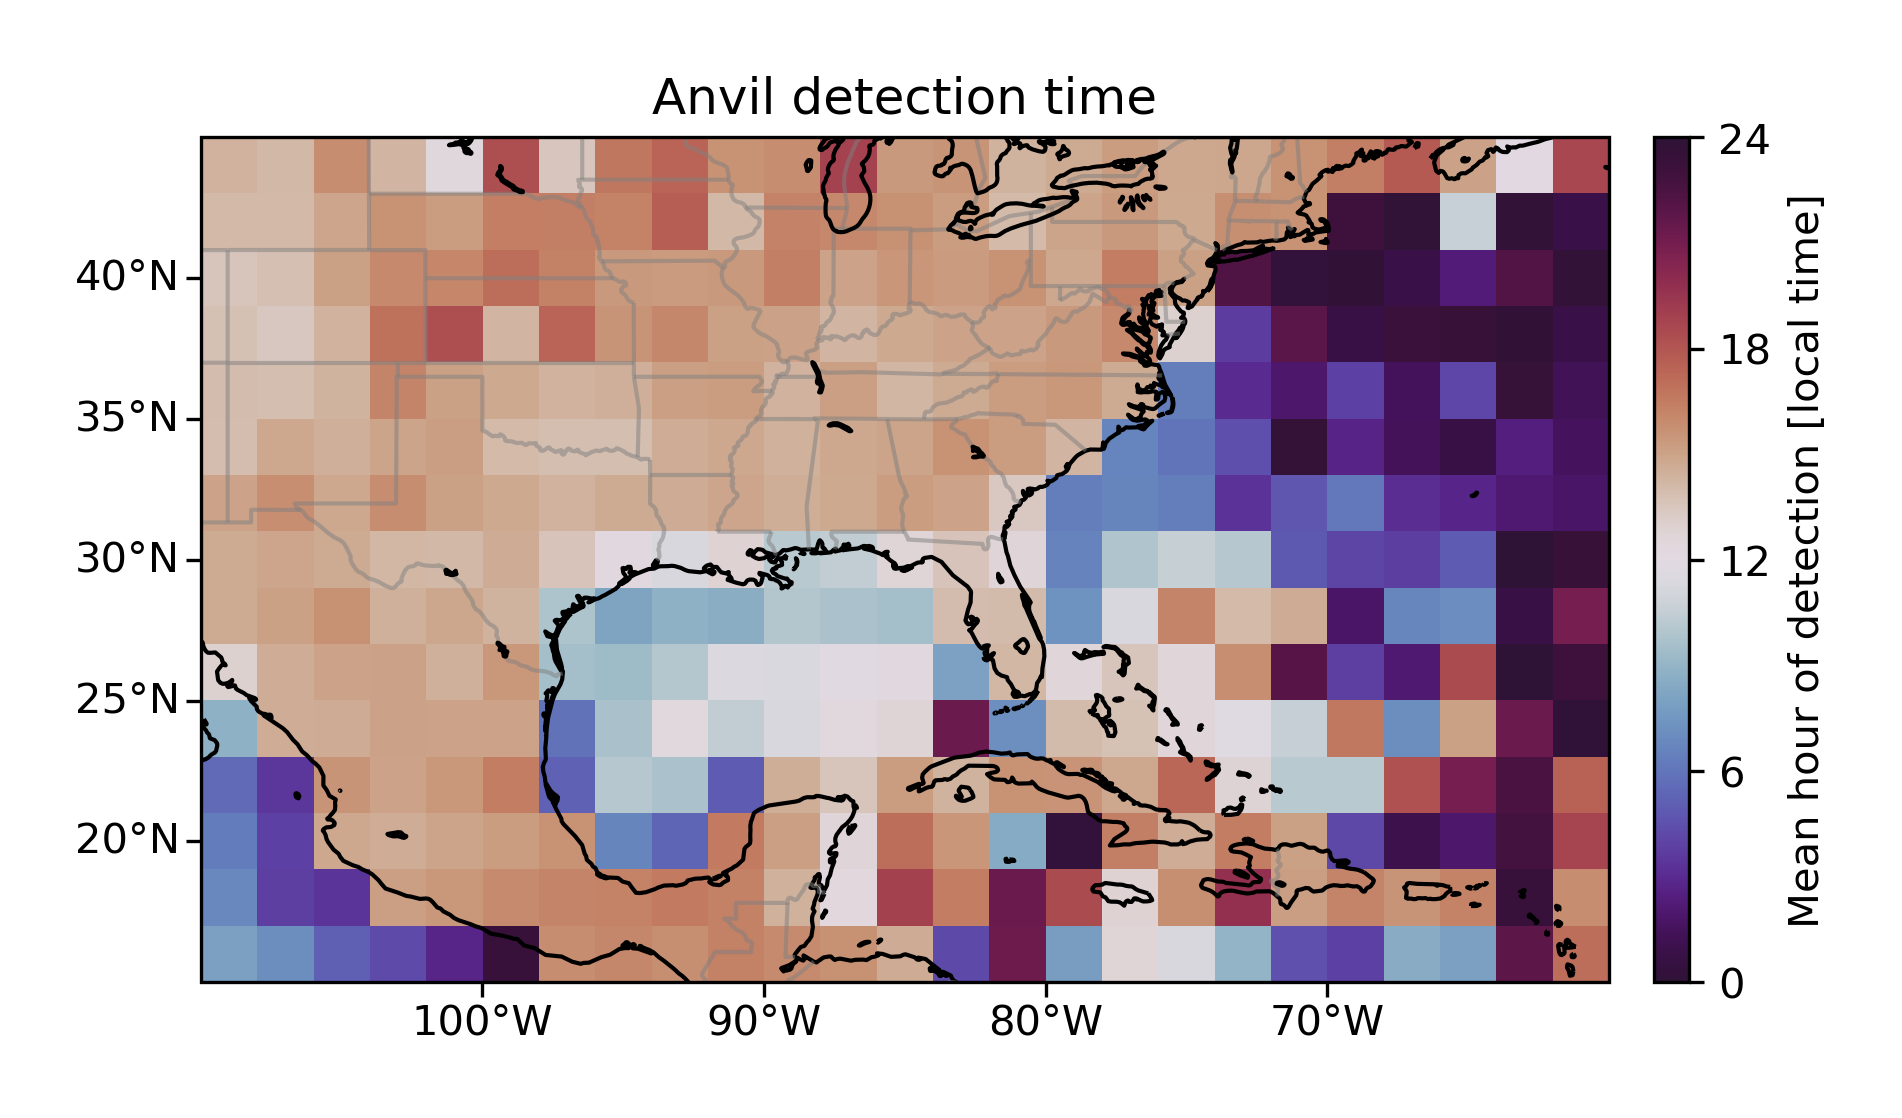
\includegraphics[width=\textwidth]{figures/chapter2_23.png}
    \caption[
    The average time of detection of anvils
    ]{
    The average time of day of detection of anvils observed within each 2\texttimes2\textdegree\ grid box, calculated as the circular mean of the local solar time.
    }
    \label{fig:anvil_detection_time_map}
\end{figure}

Figure~\ref{fig:anvil_detection_time_map} shows the average local time of day of anvil detection.
Similar to fig.~\ref{fig:core_detection_time_map} a strong land--sea contrast is seen.
However, over parts of the Caribbean Sea the average time of anvil detection is in the afternoon rather than in the morning, which may be linked to anvils that initiate over land but are advected over the ocean.
There is also a later average time of detection of anvils over the \acrshort{ngp} region, although this shows less of a contrast with surrounding land regions than that of the core initiation times.
This indicates that the second peak of core convective activity during the nighttime and early morning in fig.~\ref{fig:core_ngp_contrast} is linked to long-lived, multiple core systems including \acrshort{mcs}s, similar to what was found by \citet{feng_spatiotemporal_2019}.

%f
\begin{figure}[tp]
    \centering
    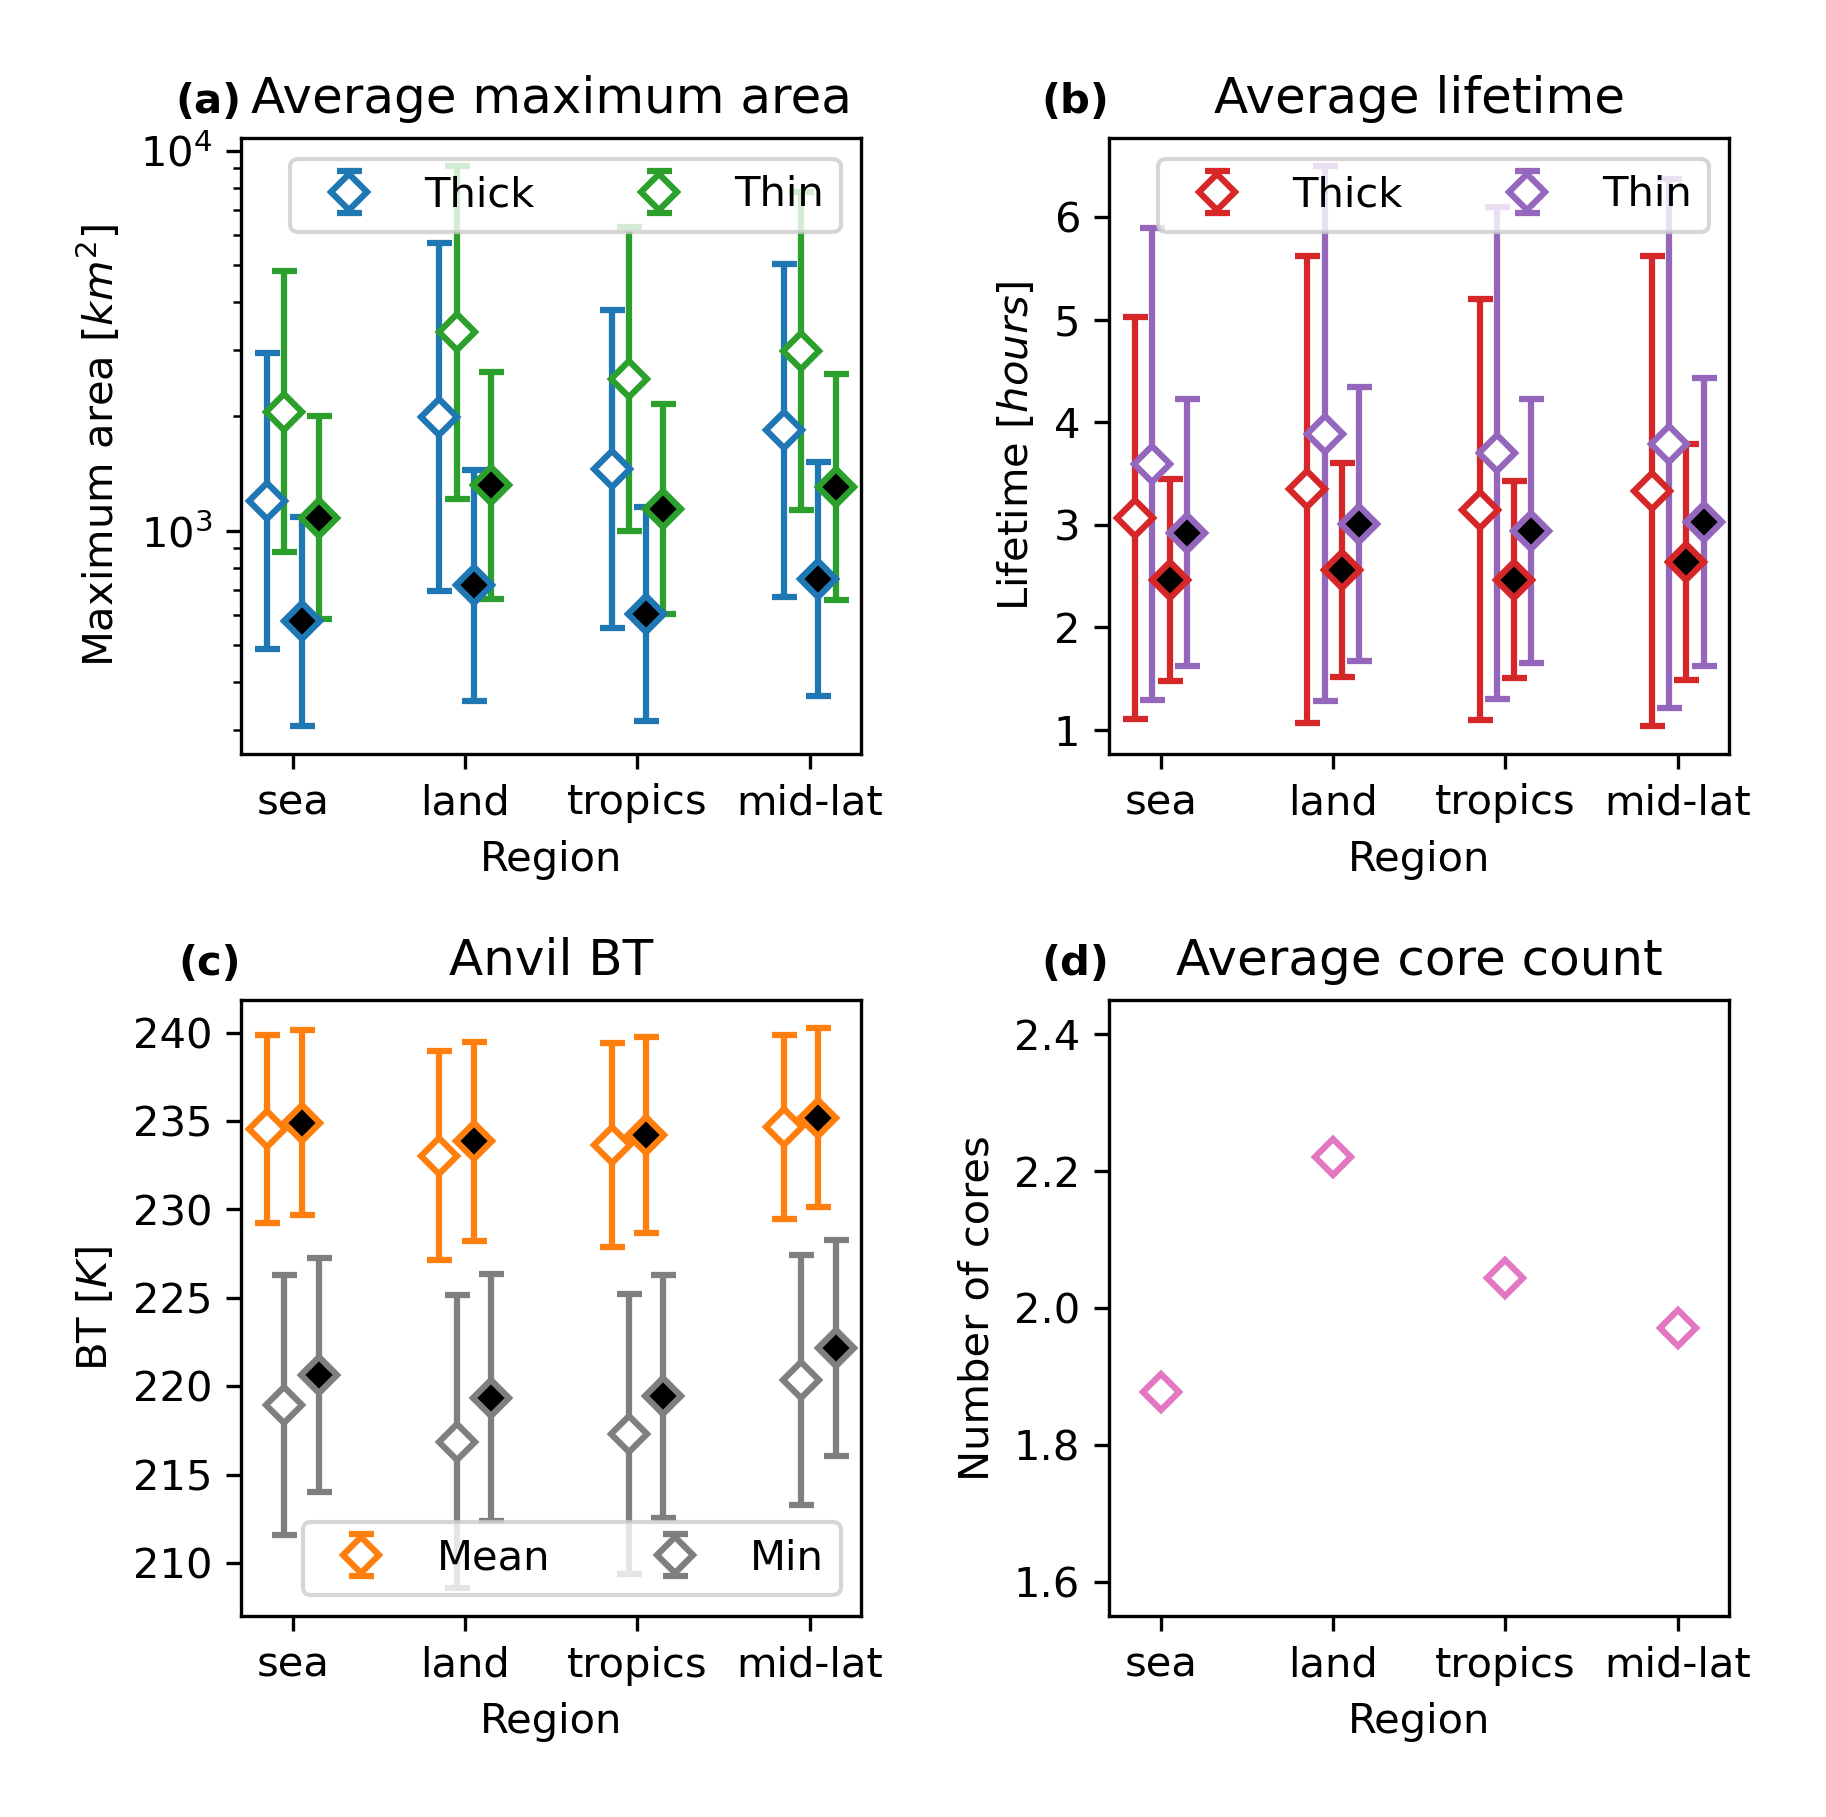
\includegraphics[width=\textwidth]{figures/chapter2_24.png}
    \caption[
    The diurnal distributions of the local time of detection for anvils detected over sea, land, tropics and mid-latitudes
    ]{
    The diurnal distributions of the local time of detection for anvils, binned by hour detected over (a) sea, (b) land, (c) tropics (\textless 30\,\textdegree N) and (d) mid-latitudes (\textgreater 30\,\textdegree N). The hatched area shows the proportion of each distribution associated with multi-core anvils.
    }
    \label{fig:anvil_diurnal_distributions}
\end{figure}

In fig.~\ref{fig:anvil_diurnal_distributions} the diurnal cycles of anvil detections are plotted by region.
The distributions generally match those seen of the core detection times shown in fig.~\ref{fig:core_diurnal_land_sea}, as the majority of the observed anvils are isolated systems.
The diurnal cycle of anvil detections over sea is much less pronounced however, which may lead to the increased variability seen in fig.~\ref{fig:anvil_detection_time_map}.
When comparing the hatched areas, indicating the proportion of the distribution consisting of multi-core anvils, over land, tropics and mid-latitudes the initiation of these organised systems occurs earlier in the day compared to isolated \acrshort{dcc}s.

%f
\begin{figure}[tp]
    \centering
    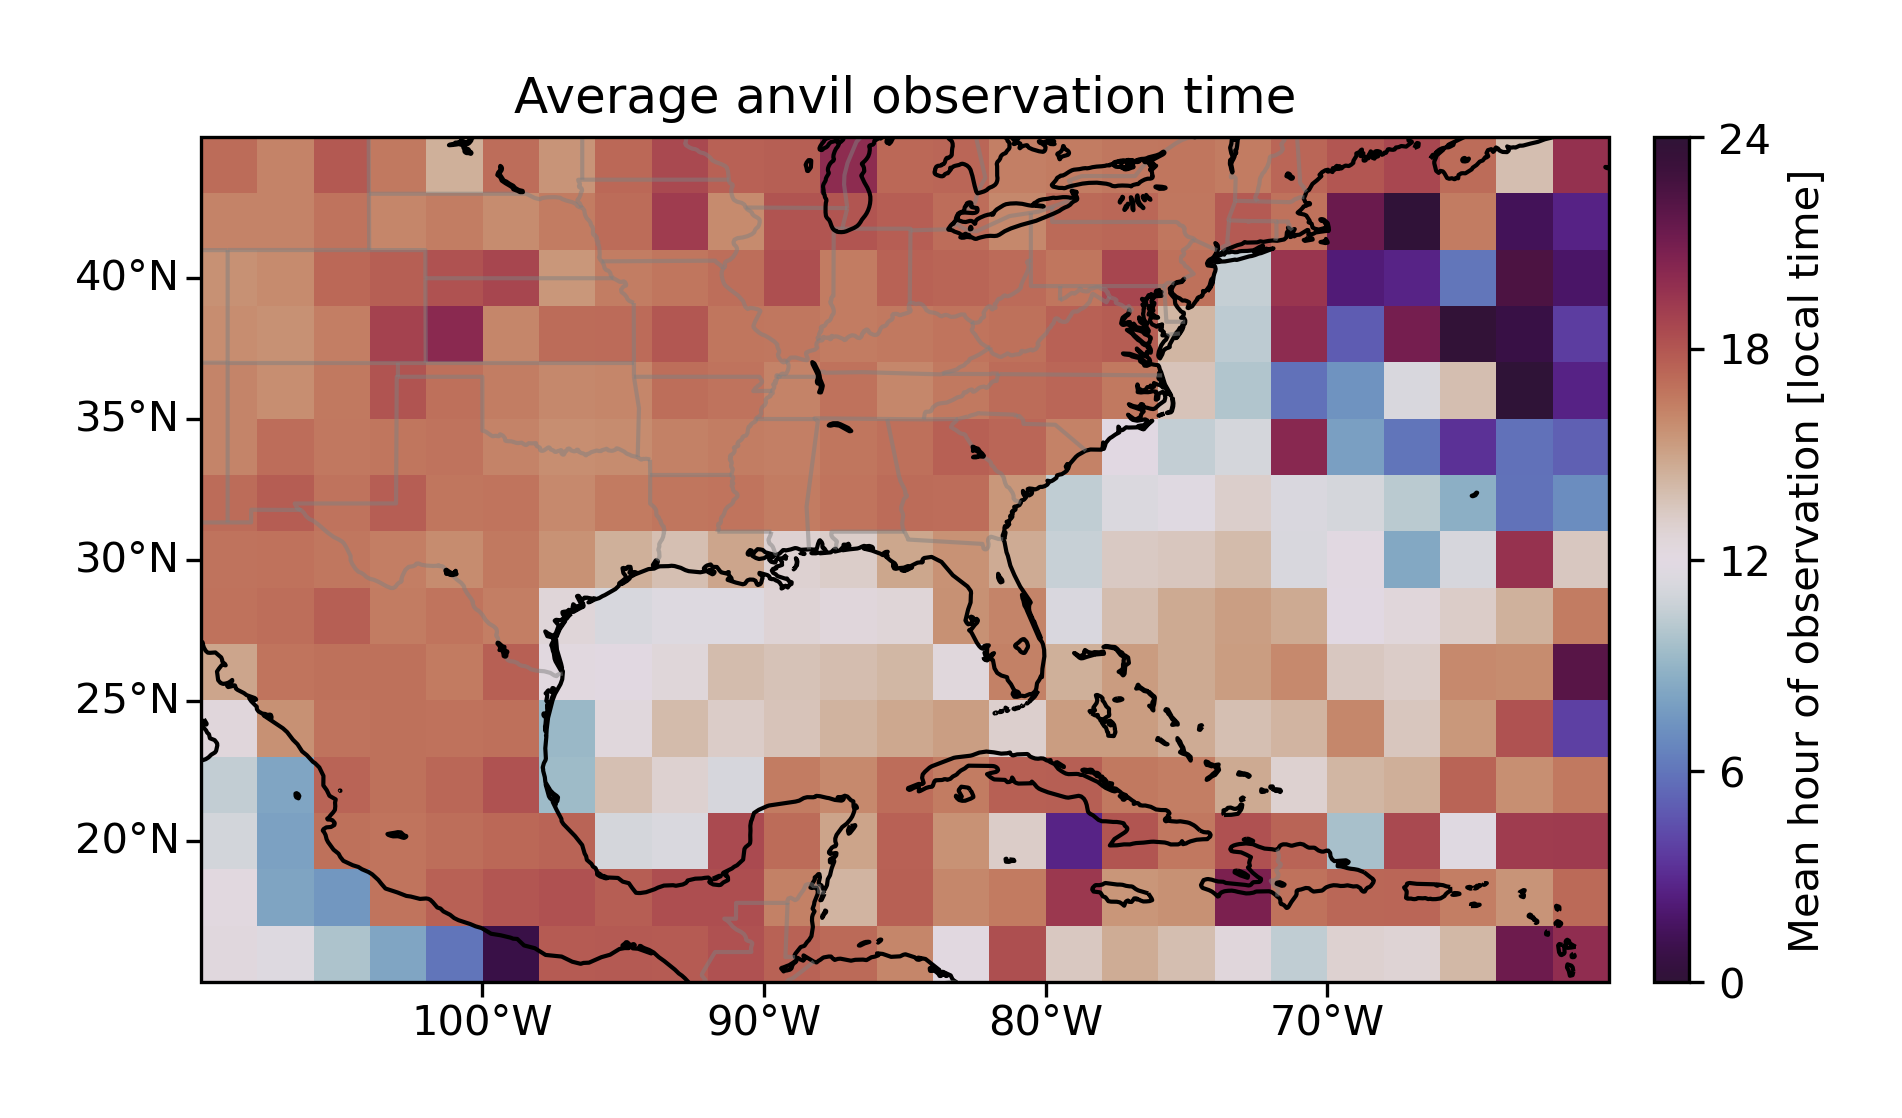
\includegraphics[width=\textwidth]{figures/chapter2_25.png}
    \caption[
    A map showing the average time of observation of anvils
    ]{
    The average time of day of observation of anvils observed within each 2\texttimes2\textdegree\ grid box, calculated as the circular mean of the local solar time. Unlike fig.~\ref{fig:anvil_detection_time_map}, this is the average of the time of observation at every time step along the anvil lifetime.
    }
    \label{fig:anvil_observation_time_map}
\end{figure}

Figure~\ref{fig:anvil_observation_time_map} shows the average time of observation for anvils.
Unlike the previous map of detection time shown in fig.~\ref{fig:anvil_detection_time_map}, in this figure the average of all the time steps at which an anvil is detected is shown.
Over the land, the effect is to shift the timing of the maximum to a later point in the diurnal cycle, which is a shift of approximately half the average anvil lifetime.
Over sea, however, there is a much larger shift with much of the Caribbean showing a similar time of day to adjacent land regions.

%f
\begin{figure}[tp]
    \centering
    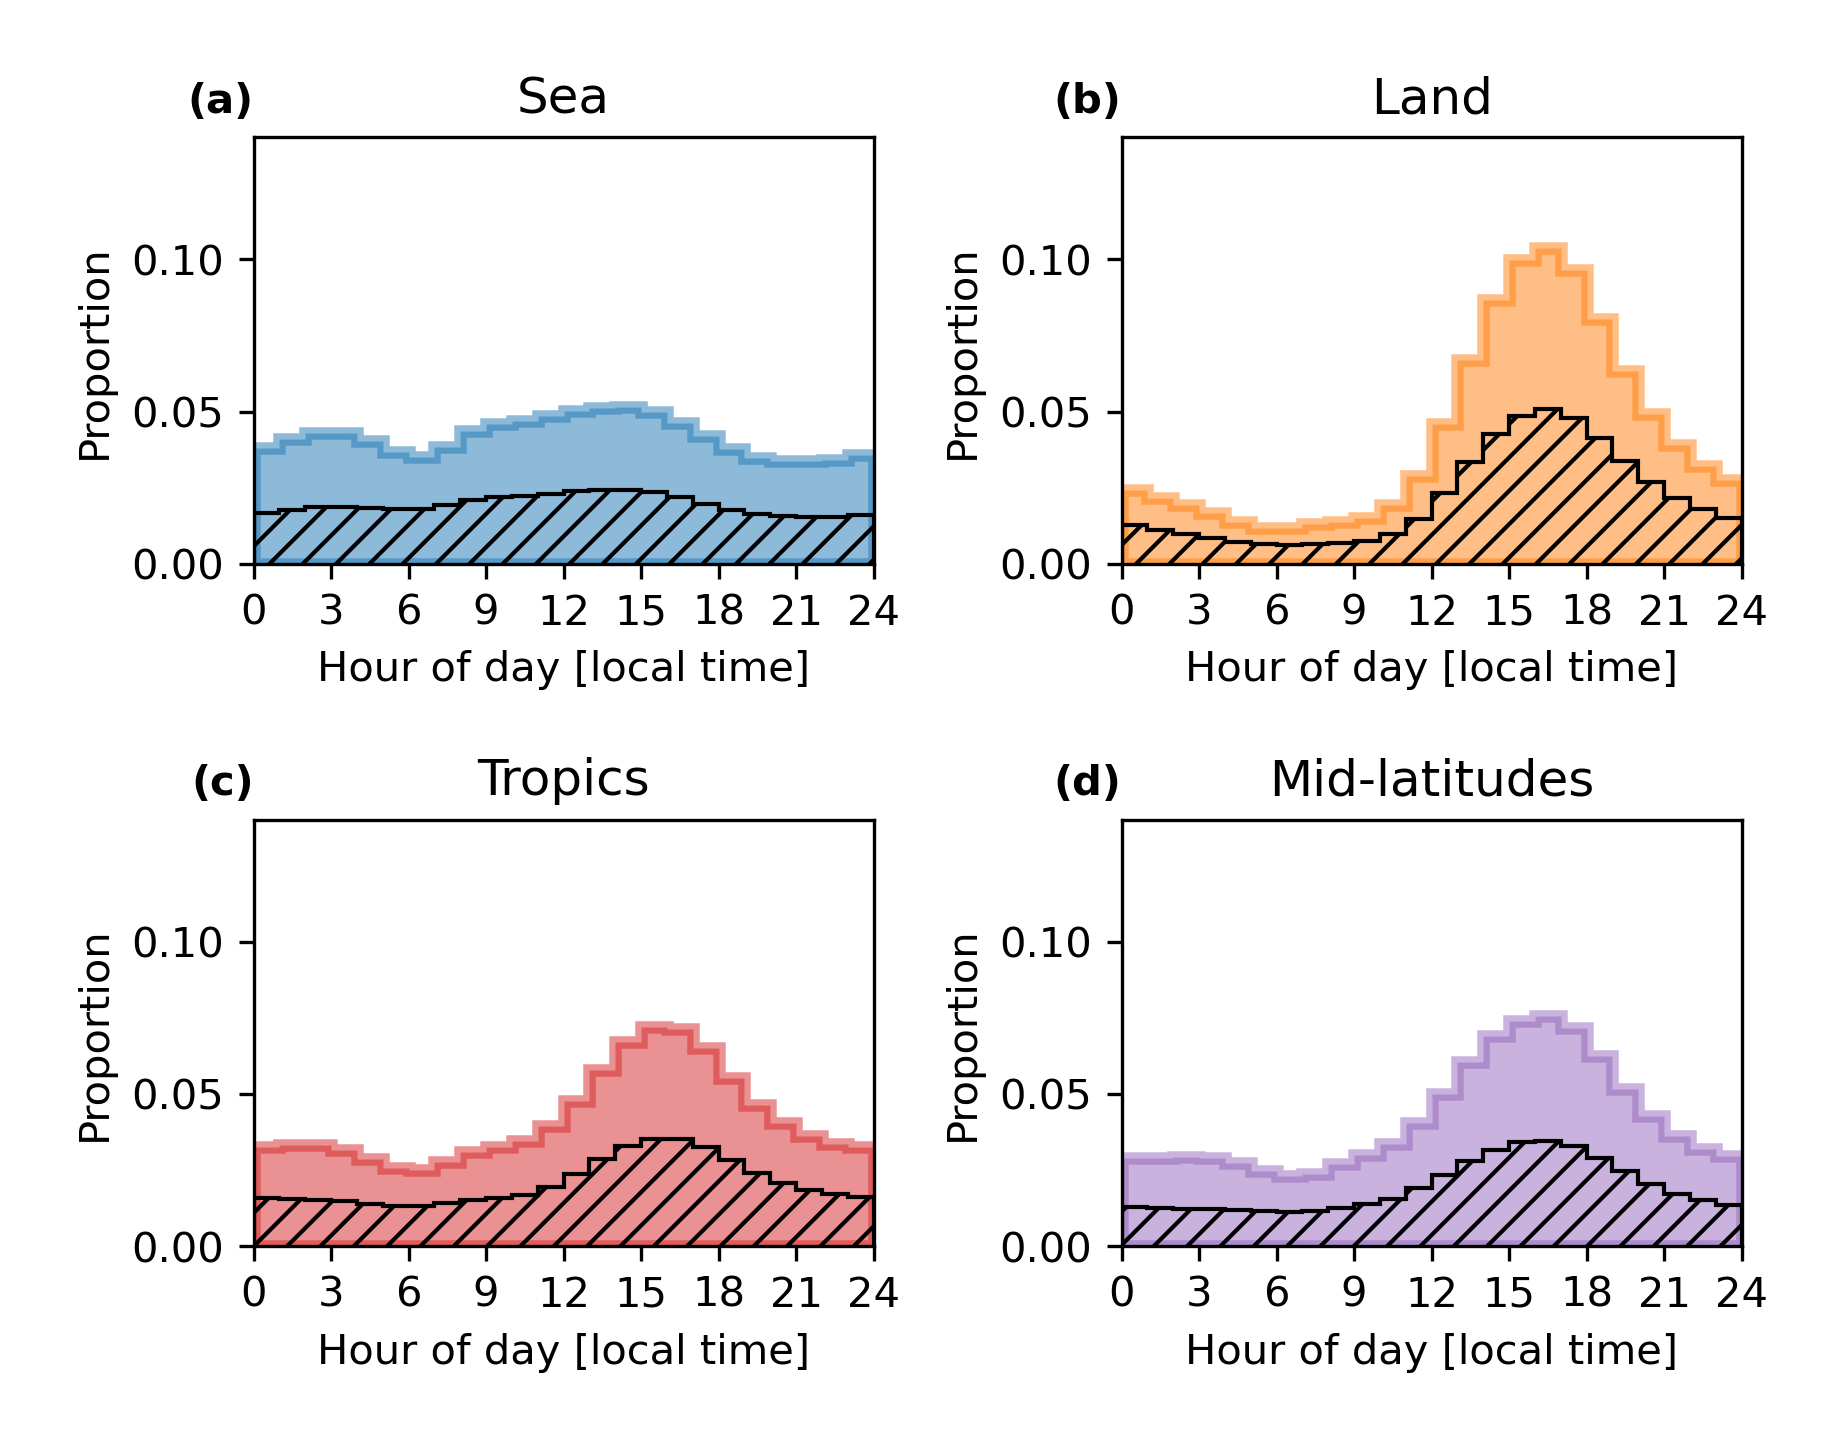
\includegraphics[width=\textwidth]{figures/chapter2_26.png}
    \caption[
    The diurnal distributions of the local time of observation for anvils detected over sea, land, tropics and mid-latitudes
    ]{
    The diurnal distributions of the local time of observation for anvils, binned by hour detected over (a) sea, (b) land, (c) tropics (\textless 30\,\textdegree N) and (d) mid-latitudes (\textgreater 30\,\textdegree N). The hatched area shows the proportion of each distribution associated with multi-core anvils.
    }
    \label{fig:anvil_diurnal_obs_distributions}
\end{figure}

Figure~\ref{fig:anvil_diurnal_obs_distributions} shows the diurnal cycle of anvil observations for each of the four regions.
For the land, tropics and mid-latitudes regions, there is a shift in the peak of the distribution to 4--5\,pm, along with a lengthening of the right tail of the distribution.
The distribution of multi-core anvils appears to match that for all \acrshort{dcc}s.
While in fig.~\ref{fig:anvil_diurnal_distributions} the initiation time of these organised anvils tended to be earlier in the day, their longer lifetime means that they tend to exist, on average, at the same times.
However, this longer lifetime also means that organised \acrshort{dcc}s make up a larger proportion of anvil observations during the nighttime and morning, and fewer during the afternoon during the peak in isolated \acrshort{dcc}s.
In fig.~\ref{fig:anvil_diurnal_obs_distributions}\,a, the peak of the diurnal distribution over the sea is in the afternoon, with a gradual increase of observations throughout the day.
Previous research has shown that solar heating during the daytime increases the area and lifetime of anvils \citep{gasparini_diurnal_2022}, which may explain why there are more anvils observed during the day, despite more initiations occurring at night.

%f
\begin{figure}[tp]
    \centering
    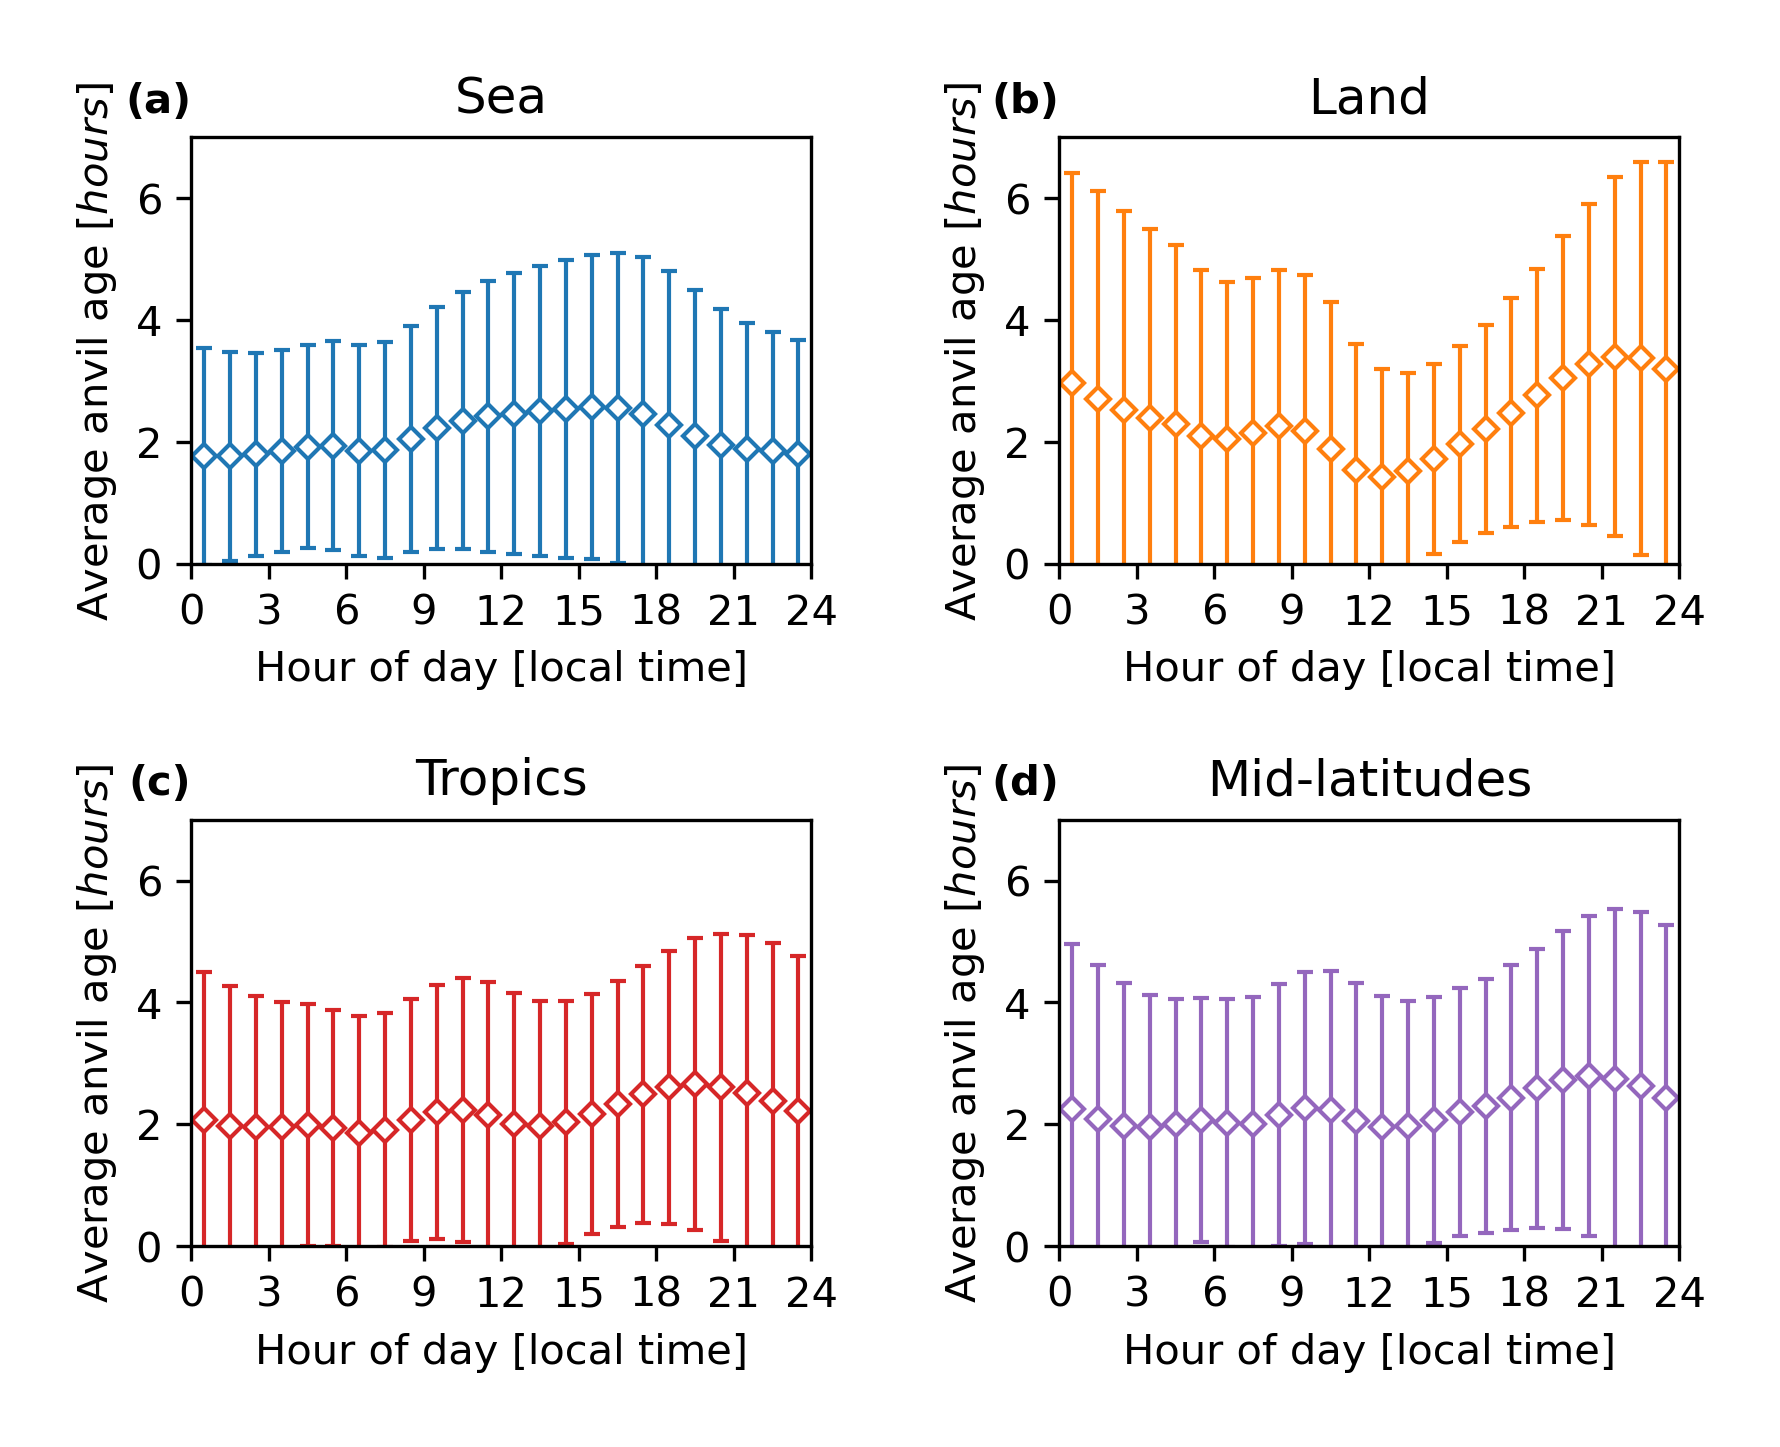
\includegraphics[width=\textwidth]{figures/chapter2_27.png}
    \caption[
    The average age of anvils observed over sea, land, tropics and mid-latitudes throughout the diurnal cycle.
    ]{
    The average age of anvils observed over (a) sea, (b) land, (c) tropics (\textless 30\,\textdegree N) and (d) mid-latitudes (\textgreater 30\,\textdegree N) throughout the diurnal cycle. Error bars show the standard deviation of the mean.
    }
    \label{fig:anvil_diurnal_age}
\end{figure}

The difference in the distributions of anvil initiation times and anvil observation times indicates that the lifetime and age of observed anvils changes across the diurnal cycle.
Figure~\ref{fig:anvil_diurnal_age} shows the average age of anvils observed during each hour of the diurnal cycle.
The increase in the age of anvils observed over sea throughout the daytime provides further evidence for the enhancement of anvil lifetime by \acrshort{sw} radiation.
For anvil observations over land, there is greater interaction with the diurnal cycle of convection.
In fig.~\ref{fig:anvil_diurnal_age}\,b there is a minima of the anvil age between midday and 1\,pm, coinciding with the onset of the afternoon peak of anvil initiations seen in fig.~\ref{fig:anvil_diurnal_distributions}\,b.
The age then increases to a maximum at around 10\,pm, before decreasing again until midday.
The variation in the average age of observed anvils is larger over land than over the ocean.
Over the tropics and mid-latitudes however, the combination of opposite signals from sea and land means that there is much less variation of anvil age across either region.


\section{Summary}  %% \conclusions[modified heading if necessary]

By applying the \textit{tobac-flow} algorithm to five years of multi-channel \acrshort{bt} observations from the \acrshort{goes}-16 \acrshort{abi} \acrshort{conus} scan region, an extensive dataset of \acrshort{dcc} cores and anvils has been produced, including their properties over time.
Containing approximately 1.6 million cores and 400 thousand anvils which are considered valid for analysis over their entire lifecycle, this dataset provides valuable information about their properties, distributions and lifecycle in a Lagrangian framework.
With five-minute temporal resolution, the properties of developing convective cores can be measured accurately, and then linked to the subsequent evolution of the anvil cloud.

A number of key differences in the seasonal, diurnal and regional patterns are seen for \acrshort{dcc}s across North America.
The spatial distribution of \acrshort{dcc} cores depends strongly on the seasonal cycle.
There is a large land/sea contrast in time of initiation, which also displays a sea breeze effect which extends for approximately 200\,\unit{km} inland.
The properties of cores themselves, including the lifetime, cooling rate, and time of initiation, have regional dependencies, with more intense convection occurring over land during the daytime and in the tropics.

These differences extend to the anvils produced by these convective cores.
The seasonal and diurnal cycles of anvils are closely related to those of the convective cores.
Furthermore, there are differences in the properties of anvils between different regions corresponding to differences in convective properties.
In particular, \acrshort{dcc}s over land have larger areas, longer lifetimes and colder \acrshort{bt} than those over the ocean.

While the majority of observed anvil clouds are associated with a single growing core, there are also a large number of multi-core anvils detected in our dataset.
The frequency of multi-core anvils as a proportion of all observed anvils increases with latitude.
Finally, while the properties of the individual growing cores observed in single- and multi-core anvils show no significant difference, the lifetime and area of anvils show a large increase with the number of cores.

Some of these findings, such as the larger area of \acrshort{dcc}s over land, contrast with studies made using polar-orbiting satellites \citep{ge_contrasting_2024}.
However, our investigation of the age of anvils observed throughout the diurnal cycle provides a mechanism for this discrepancy.
The area of \acrshort{dcc} anvils evolves as they age \citep{futyan_deep_2007}.
Impacts of radiative heating and the diurnal cycle act to modify this however \citep{gasparini_diurnal_2022}.
As a result, the average age of observed anvils varies throughout the day.
At the time of the Cloudsat overpass (1:30\,pm), the average age of anvils over land is at its minima, while those over the ocean are near their maxima.
As a result, the average area of anvils observed at this time over land would be smaller than those over the ocean, not because of a difference in their processes but because they are being observed earlier in their lifetime before they have reached their maximum area.
While at the nighttime overpass time (1:30\,am) the average age of anvils over land is older, the reduced number of land \acrshort{dcc}s at this time means that any set of snapshot observations will be biased towards younger anvils over land.

By using temporally resolved observations, and placing these in a Lagrangian framework using cloud tracking, these changes in convective cloud behaviour can be accounted for across the diurnal cycle.
Furthermore, linking the properties of the developing cores to the resulting anvil clouds over their entire lifetime provides the potential to investigate how the processes of the former affect the latter.
Connecting these properties allows investigation of previously uncertain \acrshort{dcc} processes, and, in particular, may help shed light on how anvil optical properties, structure and diurnal cycle respond to climate change.

\chapter{Contrasting effects of core intensity and organisation on the lifecycle and thin anvil extent of \acrshort{dcc}s} \label{chp:anvil_structure}

\section{Introduction}

Understanding how the structure of anvil clouds changes in response to changes in convective behaviour is vital to understanding climate feedbacks of \acrshort{dcc}s.
Around 50\% of cirrus clouds in the tropics originate from deep convection \citep{massie_distribution_2002, luo_characterizing_2004}.
Overall, anvil clouds have a near-neutral radiative impact on the tropics, despite their large \acrshort{sw} reflectance and \acrshort{lw} absorption \citep{hartmann_effect_1992, hartmann_tropical_2016}.
Their radiative effect is not homogeneous however; while the optically thick portion of anvil clouds generally have a cooling effect on the \acrshort{toa} radiative balance, the thin, detrained cirrus has a strong warming effect \citep{berry_cloud_2014}.
As a result, changes in convective activity that result in a change in the size and structure of anvil clouds may have large impacts on the climate.

The change of anvil cloud area in response to warming---the iris effect \citep{lindzen_does_2001, bony_thermodynamic_2016}---is generally considered to have a cooling feedback in response to climate change.
However, it is the largest source of uncertainty in cloud--climate feedbacks, with around a third of models predicting a warming response \citep{sherwood_assessment_2020}.
To address this uncertainty, a better understanding of the links between convective processes and anvil properties, changes in anvil structure and the properties of ice clouds are required \citep{gasparini_opinion_2023}.

Assessing the extent of thin anvil cirrus is challenging due to the difficulties in observing these clouds using \acrshort{ir} radiometers.
The low emissivity of thin cirrus clouds means that observed \acrshort{bt} is dominated by radiances from the lower atmosphere and surface below.
\citet{protopapadaki_upper_2017} used cloud emissivity and cloud top pressure, rather than \acrshort{bt}, to detect convective cores, thick and thin anvil cirrus clouds.
Data from the AIRS instrument was used to retrieve these emissivity values, as the hyperspectral sounder is more sensitive to thin cirrus than \acrshort{ir} radiometers.
They then compared the proportion of each anvil cloud consisting of thin anvil to the minimum observed cloud top temperature within the convective core, a proxy for the convective depth which is, in turn, a proxy for convective intensity.
It was found that the thin cirrus anvil proportion increased with colder cloud top temperatures, indicating that stronger convection increases the detrainment of thin cirrus.

\citet{takahashi_relationships_2017} built upon this study using collocated measurements from the \acrfull{cpr} aboard CloudSat.
The \acrshort{cpr} measurements provide the echo top height, measuring the convective depth directly, and also provide another proxy for convective intensity, the echo top distance, which is independent of convective depth \citep{takahashi_characterizing_2014}.
It was again found that the proportion of thin cirrus increased with the echo top height, and also increased with decreasing echo top distance (indicating stronger convection).

It should be noted that both of these studies were performed using observations from polar-orbiting satellites in the A-train, and so do not fully sample the diurnal cycle.
In addition, while both studies consider the maturity of the \acrshort{dcc}s observed, the thin anvil proportion is measured at a single point in time, and so differences in the lifetime of the thick and thin anvil cirrus are not considered.
By using geostationary satellite observations, we can investigate changes in the structure of \acrshort{dcc} anvils throughout their lifecycles, along with changes in the lifetime of both thick and thin anvils.
Furthermore, by taking into account the number of cores associated with each anvil, we can also investigate how organisation impacts anvil structure.


\section{Data}

In this chapter, we utilise the dataset of tracked \acrshort{dcc}s first presented in chapter~\ref{chp:lifecycle}.



Using the dataset of tracked anvils, we can investigate changes in the proportion of thick and thin anvil coverage considering both spatial extent and the lifecycle of the anvil cloud.


\section{Method}

\subsection{Detection of thick and thin anvils}

Observing thin cirrus anvils using satellite \acrshort{bt} is difficult due to their low emissivity.
Furthermore, \acrshort{bt} is affected both by the height of the observed cloud and its optical thickness.
As shown in fig.~\ref{fig:optical_depth_channels}, the observed \acrshort{bt} increases as optical depth decreases.
For detection using a fixed threshold, as used in many anvil detection algorithms, this means that the limit of optical depth at which the anvil is detected increases as the height of the cloud decreases.
This results in the detected anvil area varying with height, with an anvil at a lower altitude being detected as smaller than one at a higher altitude even if there size and structure are otherwise identical.
This problem with detected anvil area using \acrshort{bt} thresholds was identified as early as \citet{augustine_mesoscale_1988}, but remains a feature of many detection algorithms to this day (see e.g.\ section~\ref{sec:tracking_timeline}).

While observing the thin cirrus anvil is challenging, we have shown in section \ref{sec:anvil_detection} that by using a combination of \acrshort{bt} differences we are capable of detecting thin cirrus.
Furthermore, the use of channel differences reduces the height dependence of the detection of anvils compared to the use of a single \acrshort{bt}.
Figure~\ref{fig:bt_wvd_swd_height_od} shows simulated \acrshort{bt} observations using the libRadTran model \citep{emde_libradtran_2016}, as described in section~\ref{sec:detection_theory}.
The top panel shows simulation \acrshort{bt} observations by \acrshort{abi} at 10.4\,\unit{\mu m} at heights of 10, 12 and 14\,\unit{km} (shown by the solid, dashed and dotted lines respectively).
Also shown by the grey, dashed line is an example of the 241\,\unit{K} \acrshort{bt} threshold.
At this threshold there is substantial variance in the limit of \acrshort{od} at which anvil clouds are detected, which ranges from 1 at 14\,\unit{km} to 3 at \unit{km}.
This provides clear support for the argument made by \citet{augustine_mesoscale_1988} that the anvil area detected using this threshold is ``subjective''.

%f
\begin{figure}[tp]
    \centering
    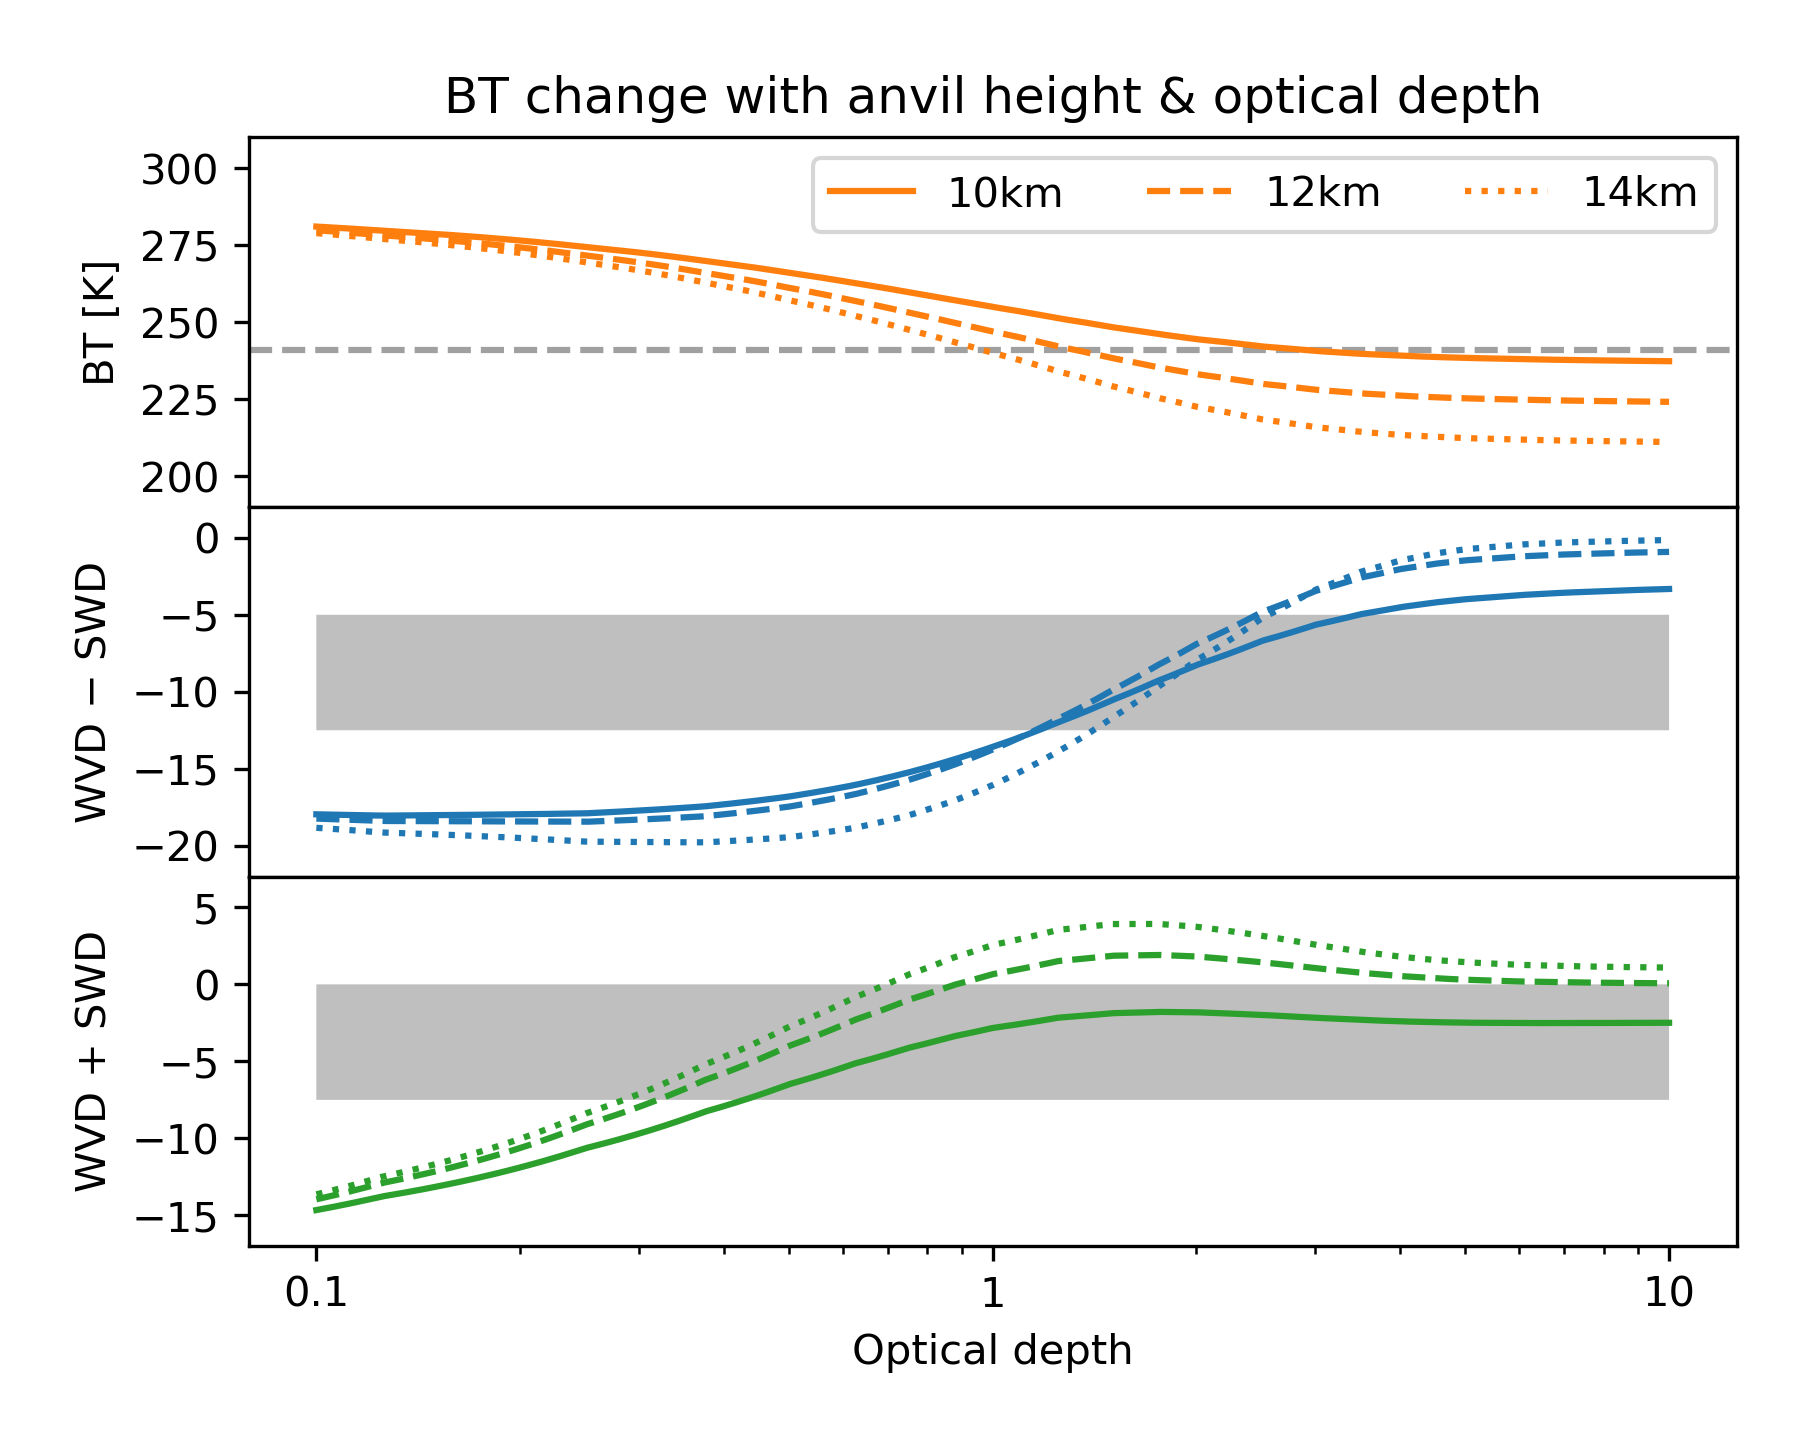
\includegraphics[width=0.9\textwidth]{figures/chapter3_01.png}
    \caption[
    Simulated \acrshort{abi} \acrshort{bt} observations of \acrshort{dcc} anvils at a range of heights and optical depths for detection of thick and thin anvil detection
    ]{
    Simulated \acrshort{abi} \acrshort{bt} observations for \acrshort{dcc} anvils at 10\,\unit{km} (solid lines), 12\,\unit{km} (dashed lines) and 14\,\unit{km} (dotted lines) at optical depths between 0.1 and 10. Panels show (top) 10.4\,\unit{\mu m} \acrshort{bt}; (middle) \acrshort{wvd} minus \acrshort{swd}, used in thick anvil detection; and (bottom) \acrshort{wvd} plus \acrshort{swd}, used in thin anvil detection. The grey dashed line shows the 241\,\unit[K] threshold, and the grey shaded regions show the range in which edge detection is performed for thick and thin anvils.
    }
    \label{fig:bt_wvd_swd_height_od}
\end{figure}

The middle and bottom panels in fig.~\ref{fig:bt_wvd_swd_height_od} show the simulated \acrshort{od} for the combinations of \acrshort{wvd} minus \acrshort{swd} and \acrshort{wvd} plus \acrshort{swd} respectively.
Section~\ref{sec:anvil_detection} describes how these two channel combinations are used for the detection of thick and thin anvils.
In both panels, the grey shaded region shows the \acrshort{bt} range in which edge detection is used to find the anvil area.
Compared to 10.4\,\unit{\mu m} \acrshort{bt}, the \acrshort{wvd} minus \acrshort{swd} combination shows very little variance in the optical depths at which the anvil cloud is detected within the threshold range.
Throughout the threshold range of --5 to --12.5\,\unit{K} the \acrshort{od} corresponding to the same observed \acrshort{bt} difference varies by approximately 0.1--0.2 between differing heights, compared to 1--2 for 10.4\,\unit{\mu m} \acrshort{bt}.

The \acrshort{wvd} plus \acrshort{swd} combination, shown in the bottom panel of fig.~\ref{fig:bt_wvd_swd_height_od}.
Greater variance between different heights is seen, particularly for the 10\,\unit{km} anvil simulation.
However, the \acrshort{od} corresponding to the observed \acrshort{bt} differences are very similar throughout the detection range of 0 to --7.5\,\unit{K} for heights of 12 and 14\,\unit{km}.
Lidar observations of thin cirrus anvil have shown that the heights of these clouds typically exceed 12\,\unit{km} \citep{wall_observational_2020, horner_evolution_2023}, and so we expect there to be little difference in the sensitivity to most observed anvils.

It should be noted that the simulations shown in fig.~\ref{fig:bt_wvd_swd_height_od} were calculated using a standard tropical atmospheric profile to best represent the moist environment in which deep convection occurs.
While anvils occurring in the extra-tropical parts of the \acrshort{conus} domain are expected to have lower cloud top heights, there is also expected to be a colder temperature profile.
As a result, we expect that the observed \acrshort{bt} for extra-tropical \acrshort{dcc}s behave more like that of the 12 and 14\,\unit{km} simulations shown in fig.~\ref{fig:bt_wvd_swd_height_od}, rather than that at 10\,\unit{km}.



\subsection{Estimation of convective intensity and organisation}


\subsection{Lifecycle analysis} \label{sec:lifecycle_definition}

\begin{figure}[tp]
    \centering
    \includegraphics[width=\textwidth]{figures/chapter3_02.png}
    \caption[
    Definition of anvil lifecycle stages based on the method of \citet{futyan_deep_2007}
    ]{
    Definition of anvil lifecycle stages based on the method of \citet{futyan_deep_2007}. The top panel shows the evolution of the mean \acrshort{bt} of the thick and thin anvil regions over the \acrshort{dcc} lifecycle, and the bottom panel shows the evolution of the anvil area. The growing phase (orange) is defined as the time between initial detection and the minimum observed \acrshort{bt}. The mature phase for the thick (blue) and thin (green) anvil is defined as the time between the minimum \acrshort{bt} and maximum thick and thin anvil area respectively. The dissipating phase for the thick (red) and thin (purple) anvils is defined as the time between the anvil maximum area and the final time of detection of the thick and thin anvil respectively.
    }
    \label{fig:lifecycle_example}
\end{figure}


To analyse changes in the lifecycle of \acrshort{dcc}s, we categorise their lifetime based on the method developed by \citet{futyan_deep_2007}.
This method separates the anvil cloud into growing, maturing and dissipating stages based on observations of \acrshort{bt} and anvil area.
\citeauthor{futyan_deep_2007}'s method defines the end of the growing phase as the time at which the anvil reaches its minimum observed \acrshort{bt}, and the end of the mature phase as the time at which the anvil reaches the maximum observed area.
While simple, this approach is applicable to a wide range of observed \acrshort{dcc}s including both isolated and organised convection.
Furthermore, by determining the anvil lifecycle only in terms of the observed anvil properties, we can treat the properties of the detected cores as independent variables allowing straightforward analysis of their impacts on lifecycle.



\section{Results}

%f
\begin{figure}[tp]
    \centering
    \includegraphics[width=0.75\textwidth]{figures/chapter3_03.png}
    \caption[
    Thin anvil proportion of anvils categorised by mean anvil \acrshort{bt}, initial core cooling rate and number of cores
    ]{
    Thin anvil proportion of anvils categorised by (a) mean anvil \acrshort{bt}, (b) initial core cooling rate, and (c) number of cores. Black error bars show the standard error of the mean, and coloured error bars show the standard deviation.
    }
    \label{fig:thin_anvil_proportion}
\end{figure}

Figure~\ref{fig:thin_anvil_proportion} shows how the observed thin area proportion of observed anvils changes in regard to observed \acrshort{dcc} properties.
In fig.~\ref{fig:thin_anvil_proportion}\,a we show how the thin anvil proportion changes with the average thick anvil \acrshort{bt} (note here that we only consider the thick anvil \acrshort{bt} to avoid a dependence between the anvil \acrshort{bt} and the thin anvil area).
We see an increase of thin anvil proportion with the average anvil \acrshort{bt}, agreeing with the results of \citet{protopapadaki_upper_2017}.
We see a larger thin anvil fraction compared to \citet{protopapadaki_upper_2017} due to observing the lifetime effects on the thin anvil, rather than comparing a single snapshot of anvil area.

Figure~\ref{fig:thin_anvil_proportion}\,b compares how the thin anvil fraction changes with the maximum cooling rate of the initial core associated with the anvil.
Here we see again that there is a positive relation between the strength of convection and the thin anvil fraction.
This also agrees with the results of \citet{takahashi_relationships_2017}, who used radar measurements of convective cores to assess the convective strength and its relationship with thin anvil area.

In fig.~\ref{fig:thin_anvil_proportion}\,c, we compare the thin anvil fraction to the number of cores associated with each anvil.
In contrast to fig.~\ref{fig:thin_anvil_proportion}\,b and c, we see a decrease in the thin anvil fraction with an increase in the number of cores.
As this occurs despite the tendency for multiple-core anvils to have colder average \acrshort{bt}, this indicates that further factors are involved in the thin anvil fraction.

In the rest of this section, we will investigate how both the core intensity and organisation impact the lifecycle anvil clouds, and how these changes influence the thin anvil fraction.

\subsection{Impact of intensity on anvil structure and lifetime}

%f
\begin{figure}[tp]
    \centering
    \includegraphics[width=0.75\textwidth]{figures/chapter3_04.png}
    \caption[
    The effect of initial core cooling rate on maximum anvil area, anvil lifetime, and mean and minimum \acrshort{bt}
    ]{
    The effect of initial core cooling rate on (a) maximum anvil area, (b) anvil lifetime, and (c) mean and minimum \acrshort{bt}. Error bars show the standard deviation. Points have been staggered to show the thick and thin anvil properties more clearly, but correspond to the same tick marks on the x axis.
    }
    \label{fig:anvil_cooling_rate_properties}
\end{figure}

%f
\begin{figure}[tp]
    \centering
    \includegraphics[width=0.75\textwidth]{figures/chapter3_05.png}
    \caption[
    The effect of the number of cores on maximum anvil area, anvil lifetime, and mean and minimum \acrshort{bt}
    ]{
    The effect of the number of cores on (a) maximum anvil area, (b) anvil lifetime, and (c) mean and minimum \acrshort{bt}. Error bars show the standard deviation. Points have been staggered to show the thick and thin anvil properties more clearly, but correspond to the same tick marks on the x axis.
    }
    \label{fig:anvil_number_of_cores_properties}
\end{figure}

We begin by investigating how the properties of observed anvil clouds change with the maximum cooling rate of their initiating core (that is, the first core observed associated with each anvil).
Figure~\ref{fig:anvil_cooling_rate_properties}\,a shows that the average thick and thin anvil maximum areas vary very little with cooling rate, except for at the highest observed values of cooling rate.
There is however a slight widening in the gap between thick and thin anvil maximum area with increasing core cooling rate.
Figure~\ref{fig:anvil_cooling_rate_properties}\,b shows that while the average thick anvil lifetime remains constant with increasing core cooling rate, the thin anvil lifetime increases.
We also see a consistent decrease in both average and minimum thick anvil \acrshort{bt} with cooling rate, shown in fig.~\ref{fig:anvil_cooling_rate_properties}\,c.


%f
\begin{figure}[tp]
    \centering
    \includegraphics[width=\textwidth]{figures/chapter3_06.png}
    \caption[
    Distributions of anvil lifecycle binned by initial cooling rate
    ]{
    Distributions of anvil lifecycle binned by initial cooling rate. The vertical lines show the mean value of each distribution.
    }
    \label{fig:anvil_cooling_rate_lifecycle}
\end{figure}

Figure~\ref{fig:anvil_cooling_rate_lifecycle} shows the distribution of the different stages of anvil lifecycle for different bins of initial core cooling rate.
With increasing cooling rate the time of coldest mean \acrshort{bt} becomes earlier, mirroring the findings regarding the relationship between core lifetime and cooling rate found in fig.~\ref{fig:core_cooling_rate_relations}.
While the timing of the maximum thick anvil area and thick anvil dissipation show little change with cooling rate, the time of thin anvil maximum area and dissipation increase.


%f
\begin{figure}[tp]
    \centering
    \includegraphics[width=\textwidth]{figures/chapter3_07.png}
    \caption[
    The average fraction of anvil lifetime of each lifecycle stage for anvils categorised by initial core cooling rate
    ]{
    The average fraction of anvil lifetime of each of the lifecycle stages defined in section~\ref{sec:lifecycle_definition} for anvils categorised by initial core cooling rate. Each bar is normalised such that the total length of the row is equal to the mean thin anvil lifetime of its cooling rate bin.
    }
    \label{fig:anvil_cooling_rate_proportional_lifecycle}
\end{figure}

Figure~\ref{fig:anvil_cooling_rate_proportional_lifecycle} displays the average proportion of anvil lifecycle spent in each of the stages shown in fig.~\ref{fig:anvil_cooling_rate_lifecycle}.
We see again that the primary effect of core cooling rate is to reduce the growing phase and increase the thin anvil dissipation stage.
The thick anvil mature stage remains similar across cooling rate, as does the time between the thick anvil maximum area and thick anvil dissipation.
Overall, this indicates that core cooling rate primarily affects the thin anvil properties, and that the increase in the proportion of thin anvil with cooling rate  is mostly due to an increase in the thin anvil lifetime.

\subsection{Impact of organisation on anvil structure and lifetime}

In fig.~\ref{fig:anvil_number_of_cores_properties} we examine how the anvil properties change with the number of cores associated with each anvil cloud.
Figure~\ref{fig:anvil_number_of_cores_properties}\,a shows that both the thick and thin anvil maximum area increase substantially with an increasing number of cores.
However, the thin anvil area increases at a slower rate proportional to the thick anvil.
We see a similar increase in the thick and thin anvil lifetime with increasing number of cores in fig.~\ref{fig:anvil_number_of_cores_properties}\,b.

We see a similar rate of the decrease of average anvil \acrshort{bt} with the number of cores in fig.~\ref{fig:anvil_number_of_cores_properties}\,c as we did in relation to core cooling rate in fig.~\ref{fig:anvil_cooling_rate_properties}\,c.
The minimum anvil \acrshort{bt} decreases at a notably faster rate with increasing number of cores however.
Although this is indicative of an increased likelihood of overshooting cores in more organised \acrshort{dcc}s, we must also note that the larger area of these systems also makes it more likely to observe colder pixels.

%f
\begin{figure}[tp]
    \centering
    \includegraphics[width=\textwidth]{figures/chapter3_08.png}
    \caption[
    Distributions of anvil lifecycle binned by number of cores
    ]{
    Distributions of anvil lifecycle binned by number of cores. The vertical lines show the mean value of each distribution.
    }
    \label{fig:anvil_number_of_cores_lifecycle}
\end{figure}

Figure~\ref{fig:anvil_number_of_cores_lifecycle} shows how the timing of the different anvil stages changes with increasing number of cores.
In general, the lifetime of every stage of the \acrshort{dcc} lifecycle increases with the number of cores.
However, the time between the thick and thin anvil maximum area and the thick and thin anvil dissipation increase at a slower rate proportion to the lifetimes of those stages.

%f
\begin{figure}[tp]
    \centering
    \includegraphics[width=\textwidth]{figures/chapter3_09.png}
    \caption[
    The average fraction of anvil lifetime of each lifecycle stage for anvils categorised by number of cores
    ]{
    The average fraction of anvil lifetime of each of the lifecycle stages defined in section~\ref{sec:lifecycle_definition} for anvils categorised by number of cores. Each bar is normalised such that the total length of the row is equal to the mean thin anvil lifetime of its number of cores bin.
    }
    \label{fig:anvil_number_of_cores_proportional_lifecycle}
\end{figure}

Figure~\ref{fig:anvil_number_of_cores_proportional_lifecycle} shows the proportion of the overall anvil lifetime spent in the different stages for increasing number of cores, similar to that in fig.~\ref{fig:anvil_cooling_rate_proportional_lifecycle}.
Unlike fig.~\ref{fig:anvil_cooling_rate_proportional_lifecycle}, we see an increase in the growing phase with increasing number of cores, and a decrease in the thin anvil dissipation phase.
In addition, while the thick anvil maturing phase changes little with the number of cores, the time for the thin anvil to reach its maximum area is substantially shorter for \acrshort{dcc}s with the most cores.
It is a combination of the smaller proportional increase in area for the thin anvil, seen in fig.~\ref{fig:anvil_number_of_cores_properties}, and smaller proportion of the \acrshort{dcc} lifecycle spent in the thin anvil dissipating phase which account for the reduction in the thin anvil proportion for increasing number of cores seen in fig.~\ref{fig:thin_anvil_proportion}\,c.

\section{Summary}

The most interesting result from this comparison is that while the core intensity and \acrshort{dcc} organisation have similar relations to anvil \acrshort{dcc}---the most common proxy used for convective intensity in satellite studies of \acrshort{dcc}s---the have opposite effects on the anvil lifecycle in relation to the thin anvil cirrus.
While \acrshort{dcc}s with individually stronger cores tend to enhance the area and lifetime of thin anvil cirrus, more organised \acrshort{dcc}s, despite their overall larger area and lifetime, tend to produce a smaller amount of thin anvil in proportion to their thick anvil area.
These two competing effects on thin anvil proportion between two modes of convective intensity may act to control the overall amount of thin anvil cirrus produced by \acrshort{dcc}s.

\chapter{A Lagrangian Perspective on the Lifecycle and Cloud Radiative Effect of Deep Convective Clouds Over Africa} \label{chp:radiative_effect}


\section{Introduction}

\acrshort{dcc}s play a key role in the tropical atmosphere. 
Forming the ascending branch of the Hadley cells near the equator, \acrshort{dcc}s are critical to the circulation and heat transfer of the tropics (Riehl and Malkus 1958),\citep{weisman_mesoscale_2015}. 
\acrshort{dcc}s are also a cause of extreme weather events including floods, lightning and hail (Westra et al., 2014). 
\acrshort{mcs} -- large, long-lived convective systems in which the anvils of multiple convective cores combine into a single, large `cloud shield' (Chen and Houze 1996, Houze 2004, Roca et al. 2017) -- are responsible for the majority of precipitation in the tropics (Tan et al. 2015). 
Changes in the behaviour of \acrshort{dcc}s with climate change have the potential for major impacts on the atmosphere, weather and society.

\acrshort{dcc}s also exert a key influence on the temperature of the tropics through their \acrshort{cre} (\acrshort{cre}). 
Due to their size, height and depth, \acrshort{dcc} anvils have large radiative effects in both the \acrshort{sw} (\acrshort{sw}) and \acrshort{lw} (\acrshort{lw}), with both having average magnitudes in excess of 100\,\unit{W m^{-2}} (Hartmann 2016, Wall and Hartmann 2018). 
However, due to the opposite signs of these two components, the average anvil \acrshort{cre} in the tropics is approximately zero (Ramanathan et al. 1989, Hartmann et al. 1992, Stephens et al. 2018). 
Radiation is also key to the lifecycle of \acrshort{dcc}s. 
Over land, convection is typically initiated by the heating of the surface and lower troposphere by solar \acrshort{sw} radiation, resulting in a peak of convective activity in the late afternoon. 
Over the ocean, however, convection is often triggered by \acrshort{lw} cooling of the upper troposphere, and so convective activity occurs more frequently in the morning. 
However, the occurrence of convection is more uniform throughout the diurnal cycle compared to that over land (Taylor et al. 2017). 
Radiation also has an impact on \acrshort{dcc} lifecycle through the differential heating of the anvil cloud, which destabilises the anvil cloud leading to dissipation due to entrainment and evaporation. 
However, \acrshort{sw} heating of the anvil cloud top during daytime acts to stabilise and delay this process, leading to differences in anvil lifetime depending on the diurnal cycle (Sokol and Hartmann, 2020).

There are a number of hypotheses regarding the \acrshort{cre} of tropical anvil clouds that consider whether the neutral \acrshort{cre} of tropical anvils is the result of a feedback mechanism. 
The thermostat hypothesis proposes that in a warmer environment anvil clouds produce thicker cirrus which acts to cool the tropics through increased \acrshort{sw} reflectance (Ramanathan and Collins, 1991). 
The Iris hypothesis proposes an alternate negative feedback mechanism in which anvil clouds reduce in area in response to warming surface temperature (due to an increase in precipitation efficiency), resulting in greater \acrshort{lw} emission from the surrounding clear regions (Lindzen et al. 2001), however support for this effect is disputed (Del Genio and Kovari 2002, Lin et al. 2004). 
On the other hand, the \acrshort{fat} hypothesis argues that the anvil \acrshort{ctt} remains constant in a warming climate due to the tendency of tropical anvil clouds to detrain at the level at which water vapour cooling becomes inefficient (around 200 K). This would result in a positive feedback mechanism whereby anvil clouds become higher to maintain the same \acrshort{ctt} and so have a larger \acrshort{lw} \acrshort{cre} due to the warmer surface temperatures (Hartmann and Larson, 2002). 
While there is evidence that this is the case for the largest \acrshort{dcc} anvils, it is debated whether these observations are due to \acrshort{fat} or due to fixed tropopause temperature (FiTT) (Seeley et al. 2019). 
The \acrshort{phat} hypothesis argues instead that while anvil clouds will become higher with warming temperatures, an associated increase in static stability results in warmer anvil temperatures and a reduced \acrshort{lw} response compared to \acrshort{fat} (Zelinka and Hartmann, 2010). 
This reduced response more closely matches the \acrshort{lw} response of tropical clouds in global climate models. 
Some observations of tropical anvil clouds have instead suggested that warming of the surface invigorates convection, leading to higher and colder anvil \acrshort{ctt} and a stronger \acrshort{lw} warming response (Igel et al., 2014).

These hypotheses however only consider changes in anvil properties such as area, reflectance and temperature, and \acrshort{fat} and \acrshort{phat} only consider the \acrshort{lw} feedback. 
Changes to the lifecycle and diurnal cycle of deep convection may also be an important factor, in particular when considering the \acrshort{sw} feedback. 
Deep convection over land may be perturbed in particular by factors which influence \acrshort{sw} fluxes, such as aerosols. 
Observations have shown that the increase in tropical precipitation can be attributed to an increase in the frequency of deep convection, rather than an intensification of individual \acrshort{dcc}s (Tan et al. 2015).

In this article, we investigate how the lifecycle of deep convection impacts the \acrshort{cre} of anvil clouds. 
To do so, we use a novel cloud tracking methodology in conjunction with derived all-sky and clear-sky radiative fluxes to characterise the \acrshort{cre} over the lifecycles of individual anvil clouds. 
This methodology is applied to 4 months of data produced for the \acrshort{esa} Cloud-\acrshort{cci}+ project over sub-Saharan Africa. 
This dataset allows us to investigate both the \acrshort{cre} of individual \acrshort{cre}s, as well as the net anvil \acrshort{cre} over the entire region. 
We find that the overall distribution of anvil \acrshort{cre} is determined by the relationship between \acrshort{dcc} lifecycle and the diurnal cycle of the \acrshort{sw} \acrshort{cre}, and discuss the implications of this for the response of \acrshort{dcc}s to a changing climate.

\section{Data}

For this case study, we used data from the \acrshort{seviri} (Schmid 2000) aboard the \acrshort{msg} Meteosat-11 satellite, which is in a geostationary orbit above the equator at 0\textdegree W. 
We use data from 4 months (May-August 2016) over sub-Saharan Africa (approximately 18\textdegree W-46\textdegree E, 31\textdegree S-15\textdegree N) at the full resolution of \acrshort{seviri}, as well as retrieved cloud properties and derived broadband fluxes produced by the \acrshort{esa} Cloud-\acrshort{cci}+ project.
Calibrated \acrshort{bt} from \acrshort{seviri} is used by the tracking algorithm, and calibrated reflectances and \acrshort{bt} are used by the cloud retrieval.

\acrshort{seviri} is a visible and infra-red (IR) radiometer with a nadir spatial resolution of 3km and a temporal sampling time of 15 minutes for the full earth disc. 
\acrshort{seviri} has 12 channels across the visible, \acrshort{nir} and thermal-IR spectrum, with one being a high-resolution visible channel with a nadir resolution of 1km. 
A brief overview of these channels, along with which are used for tracking \acrshort{dcc}s and the cloud properties retrieval, is provided in table~\ref{table:seviri_channels}.


\begin{table}[tb]
\centering
\begin{tabular}{lllcc}
\tophline
Channel & Wavelength (\unit{\mu m}) & Description & Tracking & Retrieval\tabularnewline
\middlehline
1 & 0.64 & Visible & & \checkmark\tabularnewline
2 & 0.81 & \acrshort{nir} & & \checkmark\tabularnewline
3 & 1.64 & \acrshort{nir} & & \checkmark\tabularnewline
4 & 3.92 & \acrshort{nir} Window & & \checkmark\tabularnewline
5 & 6.25 & Upper troposphere \acrshort{wv} & \checkmark & \checkmark\tabularnewline
6 & 7.35 & Lower troposphere \acrshort{wv} & \checkmark & \checkmark\tabularnewline
7 & 8.70 & Mid-IR window & &\tabularnewline
8 & 9.66 & Ozone & &\tabularnewline
9 & 10.8 & Clean \acrshort{lw} window & \checkmark & \checkmark\tabularnewline
10 & 12.0 & Dirty \acrshort{lw} window & \checkmark & \checkmark\tabularnewline
11 & 13.4 & CO\textsubscript{2} & & \checkmark\tabularnewline
12 & 0.6-0.9 & High-resolution visible & &\tabularnewline
\bottomhline
\end{tabular}
\caption[
\acrshort{seviri} channels and their use in the \acrshort{dcc} tracking algorithm and cloud properties retrieval
]{
\acrshort{seviri} channels and their use in the \acrshort{dcc} tracking algorithm and cloud properties retrieval.
}
\label{table:seviri_channels}
\end{table}


An example of observations from \acrshort{seviri} is shown in fig.~\ref{fig:seviri_obs_example} for 15:00:00 \acrshort{utc} on 1\textsuperscript{st} June 2016. 
A visible composite (fig.~\ref{fig:seviri_obs_example}\,a) is constructed using the 1.64\,\unit{\mu m} and 0.81\,\unit{\mu m} near-infrared and 0.64\,\unit{\mu m} visible channels for the \acrshort{rgb} channels respectively. 
In this composite, ice clouds -- which appear cyan -- can be seen over central Africa and the southern Atlantic. fig.~\ref{fig:seviri_obs_example}\,b shows the 10.8\,\unit{\mu m} brightness temperature for the same scene, showing the coldest temperatures for the high ice clouds over central Africa. 
Two combinations of channels are used for the detection of anvil clouds. 
The \acrshort{wvd} (\acrshort{wvd}), shown in fig.~\ref{fig:seviri_obs_example}\,c, consists of the 6.3\,\unit{\mu m} \acrshort{bt} minus the 7.4\,\unit{\mu m} \acrshort{bt}. 
In clear skies the \acrshort{wvd} is negative, with values around -20 to -15 K, due to the higher, and thus colder, emission height of the 6.3\,\unit{\mu m} channel. 
In high, thick clouds, however, the temperatures of the 6.3 and 7.4\,\unit{\mu m} channels converge and so the \acrshort{wvd} becomes closer to 0. 
In the cases of the highest clouds, the \acrshort{wvd} can become positive due to emission from stratospheric WV in the 6.3\,\unit{\mu m} channel. The \acrshort{swd} (\acrshort{swd}), shown in fig.~\ref{fig:seviri_obs_example}\,d, consists of the 10.8\,\unit{\mu m} \acrshort{bt} channel minus the 12.0\,\unit{\mu m} channel. 
While the \acrshort{swd} is sensitive to near-surface WV due to absorption in the 12.0\,\unit{\mu m} channel, it is also sensitive to thin ice clouds due to the difference in emissivity of ice particles between the two channels. 
While for thick clouds the \acrshort{swd} will be 0 K, for thin ice clouds the lower emission height of the 10.8\,\unit{\mu m} \acrshort{bt} channel results in a positive value of 5 K.
\acrshort{seviri} has wider wavebands for these two channels compared to newer sensors such as the \acrshort{goes}-16 \acrshort{abi}, and as such is less sensitive to the presence of thin ice clouds.


\begin{figure}[tp]
    \includegraphics[width=\textwidth]{figures/ch3_01.png}
    \caption[
    Example observations from the Meteosat \acrshort{seviri} instrument at 15:00:00 \acrshort{utc} on 2016/6/01
    ]{
    Example observations from the Meteosat \acrshort{seviri} instrument at 15:00:00 \acrshort{utc} on 2016/6/01. a: A visible composite formed using the 1.6, 0.81 and 0.64\,\unit{\mu m} channels as the \acrshort{rgb} channels respectively, with 10.8\,\unit{\mu m} \acrshort{bt} during the night-time. The scene shows a cluster of cold cloud tops (cyan) over central Africa and over the Southern Atlantic. b: 10.8\,\unit{\mu m} \acrshort{bt}. c: \acrshort{wvd} formed by the 6.3\,\unit{\mu m} channel minus the 7.4\,\unit{\mu m} channel. d: \acrshort{swd} formed by the 10.8\,\unit{\mu m} channel minus the twelve\,\unit{\mu m} channel.
    }
    \label{fig:seviri_obs_example}
\end{figure}


Retrieved cloud properties -- including optical thickness, effective radius, liquid/ice water path, \acrshort{ctt} and height -- are provided by the community cloud retrieval for climate (CC4CL) algorithm (Sus et al. 2018, McGarragh et al. 2018). 
These properties are all retrieved at the same resolution as the input \acrshort{seviri} data. Broadband fluxes are derived using the BUGSRad radiative transfer model (Stephens et al. 2001) using input cloud properties from the CC4CL retrieval and vertical temperature, moisture and trace gas profiles from ERA-5 (Hersbach et al. 2020). 
The BUGSRad model provides \acrshort{toa} and bottom-of-atmosphere (BoA) \acrshort{lw} and \acrshort{sw} radiative fluxes for both all-sky and clear-sky conditions. An example of these derived fluxes is shown in figure 2. 
Figure~\ref{fig:seviri_flux_example}\,a shows net \acrshort{toa} fluxes, with a net warming during the daytime on the Western side of the image, and a net cooling at night-time on the Eastern side. 
Figure~\ref{fig:seviri_flux_example}\,b shows the net \acrshort{toa} \acrshort{cre}, with a net cooling effect during the daytime and warming during the night-time for observed high clouds over central Africa. The \acrshort{sw} (fig.~\ref{fig:seviri_flux_example}\,c) and \acrshort{lw} (fig.~\ref{fig:seviri_flux_example}\,d) components of the \acrshort{cre} show that while the \acrshort{lw},
warming component has a smaller magnitude than the day-time, cooling \acrshort{sw} \acrshort{cre}, it remains constant during both day- and night-time.


\begin{figure}[tp]
    \includegraphics[width=\textwidth]{figures/ch3_02.png}
    \caption[
    An example of the \acrshort{toa} \acrshort{cre} derived using the radiative flux model
    ]{
    An example of the \acrshort{toa} \acrshort{cre} derived using the radiative flux model, for the same time
    as shown in fig.~\ref{fig:seviri_obs_example} (15:00:00 \acrshort{utc} on 2016/6/01). a: net \acrshort{toa} radiative flux. b: net \acrshort{toa} \acrshort{cre}. c: \acrshort{sw} downwards \acrshort{cre}. d: \acrshort{lw} downwards \acrshort{cre}.
    }
    \label{fig:seviri_flux_example}
\end{figure}


Validation of the \acrshort{seviri} broadband fluxes was performed against calibrated monthly-mean observations of \acrshort{toa} broadband \acrshort{cre} from the clouds and the earth's radiant energy system (\acrshort{ceres}) (Loeb et al., 2018) \acrshort{ebaf} climate data record. 
The results of this validation are shown in fig.~\ref{fig:flux_validation}. 
Monthly mean fluxes were calculated for \acrshort{seviri} by first calculating the mean daily fluxes over each 1\texttimes 1\textdegree grid square for days in which we have over 23 hours of observations, and then averaging these daily means over each month. 
Comparison of the net \acrshort{toa} \acrshort{cre} to \acrshort{ceres} revealed a bias of -3.67\,\unit{W m^{-2}} (Fig.~\ref{fig:flux_validation}\,a,b), consisting of a \acrshort{sw} bias of -3.04\,\unit{W m^{-2}} (Fig.~\ref{fig:flux_validation}\,c,d) and a \acrshort{lw} bias of -0.63\,\uni {W m^{-2}} (Fig~\ref{fig:flux_validation}\,e,f). 
These biases have been accounted for in all further \acrshort{cre} values given in this article.


\begin{figure}[tp]
    \includegraphics[width=\textwidth]{figures/ch3_03.png}
    \caption[
    Validation of derived broadband fluxes against monthly \acrshort{ceres}-\acrshort{ebaf} \acrshort{cre}
    ]{
    Validation of derived broadband fluxes against monthly \acrshort{ceres}-\acrshort{ebaf} \acrshort{cre}. a.: The mean difference in net \acrshort{toa} \acrshort{cre} by 1\texttimes 1\textdegree grid square. b.: A comparison of observed \acrshort{toa} net \acrshort{cre} for \acrshort{seviri} against \acrshort{ceres}, with all locations in blue, and those where we observe \acrshort{dcc} anvils in red. c.: the mean difference in \acrshort{sw} \acrshort{toa} \acrshort{cre}. d.: comparison of \acrshort{sw} \acrshort{toa} \acrshort{cre} for \acrshort{seviri} and \acrshort{ceres}. e.: the mean difference in \acrshort{lw} \acrshort{cre}. f.: comparison of \acrshort{lw} \acrshort{toa} \acrshort{cre}. The stippling in a,c,e represents the locations in which we observe \acrshort{dcc} anvils, with the size of the dots corresponding to the number of observations. The solid lines in b,d,f show the linear regression for all locations (blue) and the locations in we observe \acrshort{dcc} anvils (red), weighted by the number of observations.
    }
    \label{fig:flux_validation}
\end{figure}


\section{Method}

Detection and tracking of \acrshort{dcc}s was performed using the tobac-flow algorithm (Jones et al. 2023), which has been designed specifically to track both isolated and clustered \acrshort{dcc}s in geostationary satellite imagery over their entire lifecycle. 
While geostationary satellite imagery provides high-resolution observations over large domains and long time periods, which is ideal for studying deep convection, the inability of passive remote sensing to observe convective updrafts directly makes the detection and tracking of \acrshort{dcc}s difficult.

Algorithms for the detection and tracking of \acrshort{dcc}s can generally be split into two groups. 
Firstly, those designed for tracking deep convective cores, or isolated \acrshort{dcc}s, such as Cb-TRAM (Zinner et al. 2008, 2011) or tobac (Heikenfeld et al. 2019, Sokolowsky et al. 2023). 
These algorithms work by detecting regions of convective updraft or a proxy (such as cloud top cooling rate), and then treating these regions as point-like objects that are advected over time. 
Secondly, those designed for tracking mesoscale convective systems such as PyFLEXTRKR (Feng et al. 2022), TAMS (Núñez Ocasio et al. 2020) or TOOCAN (Fiolleau and Roca, 2013). 
These algorithms detect large regions of cold cloud tops indicating anvils, and then link them over time by overlapping regions at subsequent time steps. 
There is no `best' method for tracking all types of convection however (Lakshmanan and Smith, 2009). 
The algorithms for tracking isolated convective cells perform worse for clustered convection when the motion and shape of the \acrshort{dcc} cannot be adequately represented as a single vector. 
On the other hand, the \acrshort{mcs} tracking algorithms perform worse for smaller, isolated \acrshort{dcc}s as the motion of the anvil between time steps may mean it does not overlap with the previous step.

To approach the challenge of tracking both isolated \acrshort{dcc}s and large, clustered systems, we address the role of cloud motion in the scaling problem. 
tobac-flow first estimates the motion of \acrshort{dcc}s at each pixel using an optical-flow algorithm. 
Then, using these estimated motion vectors, we construct a semi-Lagrangian framework in which to perform the detection and tracking. 
This framework removes the problem of \acrshort{dcc} motion, allowing us to track both isolated and large \acrshort{dcc}s at the same time.

We detect growing convective cores where we observe regions of rapid cooling in the 10.8\,\unit{\mu m} \acrshort{bt} channel and the \acrshort{wvd}; the difference between the 6.2\,\unit{\mu m} and 7.3\,\unit{\mu m} channels. 
Using both differences allows us to detect growing \acrshort{dcc}s close to the surface and continue tracking them into the upper troposphere. 
We classify a core as a region of cooling temperature that has existed for at least 15 minutes and has cooled by at least 8K in a 15-minute period. 
This threshold provides a strong indicator of intense convective activity (Roberts and Rutledge 2003), and so provides an accurate detection of growing \acrshort{dcc}s. 
Starting from these convective cores, we then detect the surrounding anvil cloud using the \acrshort{wvd} field (Müller et al. 2018, 2019) and continue to detect the anvil until its dissipation, even after the core is no longer visible. 
Each anvil cloud can be associated with multiple cores, allowing us to identify cases of clustered convection. 
As we detect the cores based on cloud-top cooling, however, we can only detect the cores themselves during the growing phase, and cannot detect cores which occur underneath cold, high, anvil clouds. 
Due to the lack of sensitivity of the \acrshort{seviri} \acrshort{swd} to thin ice clouds, we only detect and track the thick portion of the anvil in this article.

An example of the cores and anvils detected by the tobac-flow algorithm is shown in fig.~\ref{fig:seviri_detection}, at 3-hourly intervals. In fig.~\ref{fig:seviri_detection}\,a, we see a large number of developing cores over central Africa. 
In fig.~\ref{fig:seviri_detection}\,b, we see more developing cores over Western Africa as the pattern of initiation has shifted with the diurnal cycle.
In fig.~\ref{fig:seviri_detection}\,c,d we observe fewer new developing cores later in the day, but the larger anvil clouds persist into the night-time.


\begin{figure}[tp]
    \includegraphics[width=\textwidth]{figures/ch3_04.png}
    \caption[
    An example of the cores and anvils (detected by tobac-flow, shown at 3-hour time intervals
    ]{
    An example of the cores (red outline) and anvils (blue outline) detected by tobac-flow, shown at 3-hour time intervals. All times are given in \acrshort{utc}.
    }
    \label{fig:seviri_detection}
\end{figure}


Over the 4-month period of the case study, we detect a total of 145,463 cores (of which 79,592 are associated with anvil clouds) and 35,941 anvils after quality controls have been applied. 
Using the detected regions of core and anvil clouds, the cloud properties and \acrshort{cre} are calculated for each \acrshort{dcc} at each time step from the retrieval and broadband fluxes data. 
The resulting dataset allows us to analyse the properties of each \acrshort{dcc} over their lifetimes from a Lagrangian perspective.

\section{Results}

\subsection{Spatial and temporal distributions}

Figure~\ref{fig:seviri_map_dists}\,a shows the frequency of core detections for each 1\texttimes 1\textdegree grid square over the period of the case study. 
The majority of observed convection occurs over the Guinea-Congo region. During the months of May-August, the ITCZ is at its northernmost extent over Africa (Nicholson 2018). 
The West African monsoon occurs during these months, with the primary band of convection located between 5-15\textdegree N (Nicholson 2009), which our observations agree with. 
We observed the maximum frequency of convection at around 6\textdegree N, 12\textdegree E over the Western High Plateau of Cameroon, with high frequencies of convection also observed over the Nigerian coastal plains to the West and the Jos Plateau in Northern Nigeria. 
High rates of convection are also observed over the coastal plains and inland highlands of Guinea, Sierra Leone and Liberia (5-12\textdegree N, 5-15\textdegree W)


\begin{figure}[tp]
    \includegraphics[width=\textwidth]{figures/ch3_05.png}
    \caption[
    Number of detected cores and average hour of core detection
    ]{
    Number of detected cores (a) and average hour of core detection (b) by 1\texttimes 1\textdegree grid box. Grid boxes in (b) with a standard deviation greater than 6 hours are single-hatched, and greater than 12 hours cross-hatched.
    }
    \label{fig:seviri_map_dists}
\end{figure}


Figure~\ref{fig:seviri_map_dists}\,b shows the average time of detection for convection in each 1\texttimes 1\textdegree grid square. 
The average is calculated as the circular mean of the local solar times of core detection in the grid square. 
Grid squares with a standard deviation greater than 6 hours (indicating a broad spread of initiation times) are given single hatching, and those with standard deviations greater than 12 hours have cross-hatching. 
The most notable feature of the time of detection is the clear contrast between land and sea. 
Convection over the land tends to occur in the afternoon (15:00-18:00), whereas over the ocean it occurs between midnight and early morning (00:00-09:00). 
Furthermore, convection over land tends to occur in a fairly narrow range of times whereas over the ocean convection occurs throughout the diurnal cycle, resulting in the hatching applied to much of the ocean region. 
There is also a noticeable lake effect on the time of convection occurring over Lake Victoria (2\textdegree S, 34\textdegree E) and Lake Tanganyika (7\textdegree S, 31\textdegree E), with convection typically observed in the early morning.

When we compare the regions of Cameroon and Nigeria (4-10\textdegree N, 6-14\textdegree E), where we detect the most cores in fig.~\ref{fig:seviri_map_dists}\,a, with the average time of detection in fig.~\ref{fig:seviri_map_dists}\,b, we see that the grid squares with more cores also tend to have an earlier average time of detection than the surrounding grid squares. 
Precipitation over the Nigerian plains and the Jos plateau is linked to South-westerly winds bringing moist, warm air from the Gulf of Guinea (Vondou et al. 2010). 
This warm air may then trigger convection both through the sea breeze effect and orographic lifting when it reaches the highlands, explaining both the higher frequency and earlier timing of convection compared to surrounding regions. 
A similar relationship between the high frequency of convection and earlier time of detection is also seen over the Guinea/Sierra Leone/Liberia region (5-12\textdegree N, 5-15\textdegree W), and may be due to the same mechanism.

It should be noted that due to the method of detection, cores that develop under existing anvils are less likely to be detected than those in clear sky regions. 
As a result, we may underestimate the occurrence of later occurring cores, particularly in regions such as the Northern Sahel where a second, night-time peak of precipitation has been observed.

For all further analysis, we consider only cores and anvils that are detected north of 15\textdegree S in order to constrain our analysis to tropical \acrshort{dcc}s.

\subsection{Anvil Cloud Properties}

To investigate how the behaviour of \acrshort{dcc} anvils is affected by their organisation, we group observed anvils based on how many cores are associated with them, from isolated \acrshort{dcc}s with one core to highly-clustered \acrshort{dcc}s (such as tropical cloud clusters and \acrshort{mcs}s) with 10 or more cores. 
Anvils with 6-9 cores, and with 10 or more cores, are grouped together to ensure that these groups have a comparable number of members for analysis.

Figure~\ref{fig:seviri_anvil_stats} shows properties related to the anvil area and lifetime linked to the number of cores. 
In fig.~\ref{fig:seviri_anvil_stats}\,a we show the average anvil maximum area for each group. 
We find that the maximum area increases approximately linearly with the number of cores, with increasingly clustered anvils having increasingly larger maximum areas, and highly clustered anvils having substantially larger anvils. 
Figure~\ref{fig:seviri_anvil_stats}\,b shows the average anvil lifetime compared to the number of cores. 
While the lifetime also increases with the number of cores, the difference between isolated and highly clustered anvils is proportionately smaller.


\begin{figure}[tp]
    \includegraphics[width=\textwidth]{figures/ch3_06.png}
    \caption[
    Anvil statistics by number of associated cores for average maximum area, average lifetime, occurrence of anvils by number of cores, and percentage of total anvil coverage
    ]{
    Anvil statistics by number of associated cores for average maximum area (a), average lifetime (b), occurrence of anvils by number of cores (c), and percentage of total anvil coverage (d). Error bars (a,b) show standard error of the mean.
    }
    \label{fig:seviri_anvil_stats}
\end{figure}


Figure~\ref{fig:seviri_anvil_stats}\,c shows the number of anvils observed with differing numbers of cores. 
We see that the vast majority of all anvils observed are isolated \acrshort{dcc}s, with over 80\% having a single detected core. 
As the number of cores increases, the number of anvils detected decreases rapidly. 
However, when considering the large increase in both anvil area and lifetime with the number of cores, the total anvil coverage for highly clustered anvils is much larger (see fig.~\ref{fig:seviri_anvil_stats}\,d). 
Despite their high frequency, isolated \acrshort{dcc}s only account for 12\% of total anvil coverage, whereas highly clustered (10+ cores) account for over 50\%. 
Previous studies have found that despite being few in number, \acrshort{mcs}s account for the majority of precipitation in Western Africa (Vizy and Cook 2018).

Figure~\ref{fig:seviri_anvil_ctt_stats}\,a shows the average mean \acrshort{ctt}, and fig.~\ref{fig:seviri_anvil_ctt_stats}\,b the average minimum \acrshort{ctt} for anvils with different numbers of cores. 
While the more clustered anvils have colder average anvil \acrshort{ctt}, this decrease plateaus around 225K. 
However, the absolute minimum observed \acrshort{ctt} within each anvil shows a much greater difference with an increasing number of cores. 
The most clustered anvils tend to have a minimum \acrshort{ctt} of around 185K, indicating the presence of overshooting tops and the most intense convection. 
Care should be taken when interpreting such low retrieved \acrshort{ctt} values due to the large uncertainty associated with sensor noise at these cold temperatures.


\begin{figure}[tp]
    \includegraphics[width=\textwidth]{figures/ch3_07.png}
    \caption[
    Anvil statistics by number of cores for average anvil \acrshort{ctt} and average minimum anvil temperature
    ]{
    Anvil statistics by number of cores for average anvil \acrshort{ctt} (a), and average minimum anvil temperature (b). Error bars (a,b) show standard error of the mean.
    }
    \label{fig:seviri_anvil_ctt_stats}
\end{figure}


Futyan and Del Genio (2007) divide the \acrshort{dcc} lifecycle into growing, mature and dissipating phases based on the time of observation of the coldest anvil \acrshort{ctt}, maximum anvil area and dissipation of the anvil. 
In fig.~\ref{fig:seviri_lifetime_dists} we show the distribution of the time taken to reach each of these lifecycle milestones for anvils separated by the number of associated cores. 
For all cases, the average time of minimum anvil \acrshort{ctt} occurs before the maximum area, indicating that the anvils continue to grow beyond the maximum of convective activity. 
As the number of cores associated with each anvil increases, the time of the coldest \acrshort{ctt} and largest area occur proportionately earlier during the lifetime of the anvil. 
As a result, these more clustered anvils spend more of their lifetime existing with warming, shrinking anvils than the isolated \acrshort{dcc}s.


\begin{figure}[tp]
    \includegraphics[width=\textwidth]{figures/ch3_08.png}
    \caption[
    The distribution of time to coldest mean anvil \acrshort{ctt}, largest anvil area and time of anvil dissipation
    ]{
    The distribution of time to coldest mean anvil \acrshort{ctt} (orange), largest anvil area (green) and time of anvil dissipation (red) for anvils grouped by number of cores. The vertical lines show the mean time for each distribution.
    }
    \label{fig:seviri_lifetime_dists}
\end{figure}


In fig.~\ref{fig:seviri_lifetime_proportions}, we compare the proportion of the overall anvil lifetime spent in each of the lifecycle phases defined by Futyan and Del Genio to the number of cores associated with the anvil. 
There is a clear trend that, as the number of cores increases, the proportion of the lifecycle spent in the growing phase decreases, and the proportion spent in the mature and dissipating phases increases.
 Although this approach to classifying the lifecycle of anvil clouds is simplistic and does not capture the complexities of large, long-lived \acrshort{dcc}s which may go through multiple cycles of growth, dissipation and re-invigoration, it can provide a useful perspective when considering the \acrshort{lw} \acrshort{cre} of \acrshort{dcc}s. 
 The time of the coldest average \acrshort{ctt} will be when the \acrshort{lw} \acrshort{cre} of the anvil cloud is at its greatest, and so can help understand the evolution of the anvil \acrshort{cre} over its lifetime.


\begin{figure}[tp]
    \includegraphics[width=\textwidth]{figures/ch3_09.png}
    \caption[
    The proportion of anvil lifetime spent in the growing, mature and dissipating phase
    ]{
    The proportion of anvil lifetime spent in the growing (orange), mature (green) and dissipating (red) phase, according the criteria used by Futyan and Del Genio (2007)
    }
    \label{fig:seviri_lifetime_proportions}
\end{figure}


\subsection{Anvil \acrshort{cre}}

Using the broadband fluxes data in conjunction with the tracked \acrshort{dcc} dataset, we are able to track how the \acrshort{sw}, \acrshort{lw} and net \acrshort{cre} evolve over the lifetime of each tracked anvil. 
Figure~\ref{fig:cre_lifecycle_examples} shows the time series of \acrshort{sw}, \acrshort{lw} and net \acrshort{cre} as well as the cumulative average \acrshort{cre} for a number of different cases of anvil lifecycles. 
Note that all fluxes are \acrshort{toa} and measured in the downward direction, so a positive value is warming and a negative value represents cooling.


\begin{figure}[tp]
    \centering
    \includegraphics[width=0.8\textwidth]{figures/ch3_10.png}
    \caption[
    Anvil net, \acrshort{lw}, and \acrshort{sw} \acrshort{cre}, accumulated mean \acrshort{cre} over anvil lifetime
    ]{
    Anvil net, \acrshort{lw}, and \acrshort{sw} \acrshort{cre}, accumulated mean \acrshort{cre} over anvil lifetime and anvil area for (a) an isolated, short-lived (4-hour) \acrshort{dcc}, (b)a moderately clustered, 1-day long \acrshort{dcc}, and (c) a large, clustered, 4-day long \acrshort{dcc}. All times are the local solar time, to the nearest 5 minute interval
    }
    \label{fig:cre_lifecycle_examples}
\end{figure}


Figure~\ref{fig:cre_lifecycle_examples}\,a shows the case of an isolated, short-lived \acrshort{dcc}. 
The \acrshort{dcc} initiates during the daytime, during which the \acrshort{sw} \acrshort{cre} dominates and the net \acrshort{cre} is negative (cooling). 
However, towards the end of the four-hour lifecycle of the \acrshort{dcc}, it transitions to night-time and so while the \acrshort{sw} \acrshort{cre} reduces and eventually becomes zero, the \acrshort{lw} \acrshort{cre} dominates and the net \acrshort{cre} is positive (warming). 
While this period of warming moves the cumulative average \acrshort{cre} towards zero, it remains overall negative for the overall lifetime of the \acrshort{dcc} both due to the longer period spent during the daytime, and the larger area of the anvil cloud during this period.

Figure~\ref{fig:cre_lifecycle_examples}\,b shows the case of a longer-lived (22 hours), clustered \acrshort{dcc}. 
It initiates in the morning, and so the \acrshort{sw} cooling dominates for the first half of the anvil lifetime. 
Compared to the isolated \acrshort{dcc}, it exists for much longer during the night time, and so the cumulative average becomes positive over the full lifetime of the anvil cloud.

Figure~\ref{fig:cre_lifecycle_examples}\,c shows the case of a four-day, highly clustered convective event. 
In this case, we see the net \acrshort{cre} alternative between warming and cooling throughout the diurnal cycle. 
The cumulative \acrshort{cre} also alternates between overall warming and cooling throughout the lifetime of the anvil and is results in a small net cooling effect.

We see in both the longer-lived cases (fig.~\ref{fig:cre_lifecycle_examples}\,b,c) that the \acrshort{lw} \acrshort{cre} reduces towards the end of the anvil cloud lifetime. 
This may be reflective of the findings from Fig. 8 that the minimum average \acrshort{ctt} occurs before the mid-point of the cloud lifecycle for longer-lived systems. 
In addition, the accumulated radiative cooling of the anvil top may drive subsidence and reduce the cloud-top height of the anvil over time (Sokol and Hartmann, 2020)

Figure~\ref{fig:anvil_cre_dist} shows the distribution of net lifetime \acrshort{cre} for all tracked anvils. 
The overall negative average value of -8.17\textpm0.85 \,\unit{W m^{-2}} is approximately zero when considering the negative bias in the broadband flux dataset. 
However, the distribution shows a bimodal structure, with two peaks at around +100\,\unit{W m^{-2}} (warming) and -180\,\unit{W m^{-2}} (cooling). 
The distribution is coloured according to the mean number of cores associated with the anvils in each bin of the distribution. 
Both the peaks of the distribution are mainly composed of isolated \acrshort{dcc}s which occur during the daytime (negative peak) or night-time (positive peak). 
The centre of the distribution -- with average \acrshort{cre}s close to zero -- shows a greater number of the clustered \acrshort{dcc}s with multiple cores which, due to their longer lifetime, tend to exist during both the day- and night time.


\begin{figure}[tp]
    \includegraphics[width=\textwidth]{figures/ch3_11.png}
    \caption[
    The distribution of lifetime anvil \acrshort{cre} for all observed anvils
    ]{
    The distribution of lifetime anvil \acrshort{cre} for all observed anvils. The mean number of cores per anvil in each bin is indicated by the colour scale. The vertical dashed line shows the integrated mean \acrshort{cre} over all anvils, weighted by the anvil areas (0.86\,\textpm\,0.91\,\unit{W m^{-2}}).
    }
    \label{fig:anvil_cre_dist}
\end{figure}


In fig.~\ref{fig:anvil_sw_lw_cre} we break down the \acrshort{cre} distribution into that of the \acrshort{sw} (fig.~\ref{fig:anvil_sw_lw_cre}\,a) and \acrshort{lw} (fig.~\ref{fig:anvil_sw_lw_cre}\,b) components. 
The \acrshort{sw} \acrshort{cre} shows a similar bimodal distribution to that of the net \acrshort{cre}, whereas the \acrshort{lw} distribution shows a normal distribution. 
The \acrshort{sw} \acrshort{cre} has a large peak at 0\,\unit{W m^{-2}} for \acrshort{dcc}s that occur during the night-time, and a broad peak centred around -300\,\unit{W m^{-2}} consisting of daytime \acrshort{dcc}s, with the average falling between the two. 
Note that the average for the \acrshort{lw} falls to the right of the peak of the distribution because the average is integrated over the anvil area and lifetime, and the largest and longest-lived anvils tend to have colder \acrshort{ctt} and hence larger \acrshort{lw} \acrshort{cre}.


\begin{figure}[tp]
    \includegraphics[width=\textwidth]{figures/ch3_12.png}
    \caption[
    The distributions of mean anvil \acrshort{sw} \acrshort{cre} and \acrshort{lw} \acrshort{cre}
    ]{
    The distributions of mean anvil \acrshort{sw} \acrshort{cre} (a) and \acrshort{lw} \acrshort{cre} (b). The vertical dashed line shows the integrated mean \acrshort{cre} over all anvils (\acrshort{sw}: -133.9\,\textpm\,0.9\,\unit{W m^{-2}}, \acrshort{lw}: 134.8\,\textpm\,0.1\,\unit{W m^{-2}})
    }
    \label{fig:anvil_sw_lw_cre}
\end{figure}


Figure~\ref{fig:anvil_cre_time_vs_ctt} shows the average net anvil \acrshort{cre} binned by intervals of time of detection and mean anvil \acrshort{ctt}. 
We see that, as expected, mean anvil \acrshort{cre} becomes more positive with increasing \acrshort{ctt}. 
However, the diurnal cycle of detection shows a much stronger contrast, with anvils detected during the daytime having a cooling effect compared to those at night. 
This diurnal cycle effect is stronger for those anvils with cooler average \acrshort{ctt}, generally representing isolated, shorter-lived \acrshort{dcc}s, and is weaker for colder anvil \acrshort{ctt}. 
Note also that the phase of the diurnal cycle shifts to earlier times of detection as average anvil \acrshort{ctt} become colder, as these \acrshort{dcc}s tend to have longer lifetimes.


\begin{figure}[tp]
    \includegraphics[width=\textwidth]{figures/ch3_13.png}
    \caption[
    Average anvil \acrshort{cre} binned by the time of detection (local time) and mean anvil \acrshort{ctt}
    ]{
    Average anvil \acrshort{cre} binned by the time of detection (local time) and mean anvil \acrshort{ctt}.
    }
    \label{fig:anvil_cre_time_vs_ctt}
\end{figure}


For anvil cloud \acrshort{cre} to be radiatively balanced, sufficient \acrshort{dcc}s must initiate during the daytime, cooling region shown in Fig. 13 to balance the warming effect of \acrshort{dcc}s initiating during the rest of the diurnal cycle. 
As anvil temperatures become colder, this region becomes narrower and shifts earlier in the day, due to both the increased \acrshort{lw} \acrshort{cre} of colder anvil clouds and also due to the tendency of these anvils to have longer lifetimes. 
As a result, if warming surface temperatures lead to the invigoration of \acrshort{dcc}s, the warming effect we would see would be larger than just that due to the change in anvil temperature alone. 
To restore the net anvil \acrshort{cre} to zero, the distribution of \acrshort{dcc}s may need to shift earlier in the diurnal cycle, leading to large changes in the patterns of convection and precipitation. 
This may also further affect the anvil lifetime, due to the differences in the anvil subsidence between day- and nighttime (Sokol and Hartmann, 2020)

\section{Summary}

By combining a novel cloud tracking algorithm with a new dataset of derived all-sky and clear-sky fluxes from geostationary satellite observations, we were able to detect and track \acrshort{dcc} anvils and their associated cores for both isolated and clustered \acrshort{dcc}s and investigate their properties, lifecycle and \acrshort{cre}. 
As this study was performed using data from May-August (Northern hemisphere summer), we observed the majority of convective activity over the Guinea-Congo rainforest and Savanna regions, as the ITCZ is at its northernmost extent.

We evaluate the degree of convective clustering of each anvil by measuring the number of cores it is associated with. 
We find that, as expected, anvils with the greatest number of cores---including \acrshort{mcs}s---have larger anvil areas, longer lifetimes and the coldest cloud tops. 
As a result, despite the majority of observed \acrshort{dcc}s being isolated, the highly clustered anvils make up most of the anvil coverage, and so cause most of the anvil impact over this region. 
We also find that the proportion of the lifecycle spent in the mature and dissipating phases increases with the number of cores, and the proportion spent in the growing phase decreases.

When looking into the net \acrshort{cre} of anvils, we find that, although the average \acrshort{cre} across all observed anvils is approximately zero, few anvils have near zero \acrshort{cre} themselves. 
We find a bimodal distribution of anvil \acrshort{cre}, with isolated \acrshort{dcc}s that occur during the daytime causing the negative (cooling) peak, and those which occur during the night-time causing the positive (warming) peak. 
The systems with near zero \acrshort{cre} tend to live longer with more cores, and exist during both the day- and night-time. 
As a result, when considering the magnitude of the anvil \acrshort{cre}, isolated \acrshort{dcc}s have an outsize contribution to the overall average anvil \acrshort{cre} of 18.7\% compared to their proportion of all anvil coverage (11.9\%).

The interaction between the diurnal cycle of convection and \acrshort{dcc} lifetime plays a key role in the shape of the \acrshort{sw} anvil \acrshort{cre} distribution and is important to consider in regard to anvil \acrshort{cre} feedback. 
As the \acrshort{lw} \acrshort{cre} is normally distributed, a response to changing cloud top height or temperature may occur as a shift in the distribution. 
However, the bimodal distribution of the \acrshort{sw} \acrshort{cre} must result in more complex adjustments to shift the overall mean. 
As the position of the peak at 0 \,\unit{W m^{-2}} relating to night-time \acrshort{dcc}s is fixed, to change the overall average \acrshort{sw} \acrshort{cre} either the width of the distribution has to increase or decrease, or the number of \acrshort{dcc}s occurring during the day- or night-time has to increase. 
The former has important implications for the diurnal cycle of temperature in the tropics, and the latter for the diurnal cycle of convection.

This highlights topics of interest for future research. 
Firstly, as this study only involved 4 months of data during the Northern Hemisphere summer, we were not able to investigate the impact of the seasonal cycle on the behaviour of \acrshort{dcc}s and their \acrshort{cre}. 
Extending this research to a full year of data over a larger domain would allow investigation of seasonal and regional differences, in particular also over the oceans. 
Secondly, an investigation of atmospheric heating effects from \acrshort{dcc}s. \acrshort{sw} and \acrshort{lw} fluxes have notably different effects on atmospheric heating, and so although the \acrshort{toa} flux may be in balance for tropical \acrshort{dcc}s, changes in the \acrshort{lw} or \acrshort{sw} \acrshort{cre} may have resulted in different heating profiles and diurnal cycles. 
In particular, anvil heating by \acrshort{lw} and \acrshort{sw} is important to anvil lifetime and dependent on the diurnal cycle (Harrop and Hartmann 2018, Sokol and Hartmann 2020), and so gaining a better understanding of this may aid in understanding the lifecycle of both isolated and clustered convection in the tropics. 
Finally, investigating the response of \acrshort{dcc} \acrshort{cre} to perturbations of the diurnal cycle of deep convection. 
Anthropogenic effects such as biomass burning aerosol radiative effect and land use change may change the diurnal cycle of deep convection over land, and as shown this may have a large influence on the \acrshort{toa} \acrshort{cre}. 
Understanding how the \acrshort{cre} of deep convection responds to changes in the diurnal cycle may be key to understanding future changes in deep convection in the tropics.

\chapter{Conclusion} \label{chp:conclusion}

%now enable appendix numbering format and include any appendices
% \appendix
% \include{appendix1}
% \include{appendix2}

\clearpage
\baselineskip=18pt plus1pt

%next line adds the Bibliography to the contents page
\phantomsection
\addcontentsline{toc}{chapter}{Bibliography}
%uncomment next line to change bibliography name to references
%\renewcommand{\bibname}{References}
\bibliography{bibliography.bib}
\bibliographystyle{apalike}  % bibliography style


\end{document}
